% 第九章 同调代数 --- 中译
% 原书 pp. 559--... (Aluffi, Algebra: Chapter 0, Chapter IX).
% 本文件进度: 第 IX 章整章闭合 ✅ (2026-09-01): §9.1 加性/Abel 范畴预备; §9.2 Abel 范畴中工作; §9.3 复形与上同调 (再探); §9.4 锥与同伦; §9.5 同伦范畴·投射/内射复形; §9.6 投射/内射分解与导出范畴; §9.7 导函子; §9.8 双复形; §9.9 谱序列/正合偶. 编译链 xelatex→biber→xelatex×2 零错误、零未解析引用、零重复标签、零 ??; main.pdf 605 页. 编号经 aux 核验与原书一致 (§9.3: 3.1–3.5/3.1–3.15; §9.4: 4.1–4.16/4.1–4.16; §9.5: 5.1–5.16/5.1–5.14; §9.6: 6.1–6.9/6.1–6.13; §9.7: 7.1–7.19/7.1–7.19; §9.8: 8.1–8.14/8.1–8.14; §9.9: 9.1–9.5/9.1–9.10).

\chapter{同调代数}
\label{chap:homological-algebra}


% ===== 记号索引 v1 集中埋点 (页码参考原书书页; 首次出现位置待人工校对) =====
% 本章记号条目（16 条）。OCR 已做最佳校正，但部分符号字形与首次
% 出现位置仍待逐条人工复核（页码沿用原书第 699 页 Index of Notation）。
% ===== /记号索引 =====
\index[sym1]{$C(A)$@$C(A)$}
\index[sym1]{$D(A)$@$D(A)$}
\index[sym1]{$I$@$I$}
\index[sym1]{$\id(B)$@$\id(B)$}
\index[sym1]{$\cate{K}(\cate{A})$@$\cate{K}(\cate{A})$}
\index[sym1]{$\cate{K}^+(\cate{I})$@$\cate{K}^+(\cate{I})$}
\index[sym1]{$\cate{K}^-(\cate{P})$@$\cate{K}^-(\cate{P})$}
\index[sym1]{$\mathbb{L}^\times$@$\mathbb{L}^\times$}
\index[sym1]{$\cate{MC}(\mathcal{I})^\bullet$@$\cate{MC}(\mathcal{I})^\bullet$}
\index[sym1]{$\cate{MC}_{\mathrm{yl}}(\mathcal{I})^\bullet$@$\cate{MC}_{\mathrm{yl}}(\mathcal{I})^\bullet$}
\index[sym1]{$P$@$P$}
\index[sym1]{$\pd(A)$@$\pd(A)$}
\index[sym1]{$R^*$@$R^*$}
\index[sym1]{$\mathrm{Seq}(\cate{A})$@$\mathrm{Seq}(\cate{A})$}
\index[sym1]{$\cate{TC}(M)^\bullet$@$\cate{TC}(M)^\bullet$}
\index[sym1]{$v\mathbb{E}_i^{(j)}$@$v\mathbb{E}_i^{(j)}$}
我们在第八章 §VIII.\ref{sec:tensor-tor} 与 §VIII.\ref{sec:projective-injective-ext} 中对 Tor 与 Ext 函子所作的有限接触, 应当能在读者偶尔碰到这两个函子时有所帮助. 然而, 很有必要回过头来, 把所有的 i 点上点, 把所有的 t 画上横线, 以便证明那些造就了这两个函子之存在与性质的精彩事实.
这是本章所涵盖素材的一个动机. Tor 与 Ext 是\emph{导函子} (derived functor) 的实例, 而导函子是一套能让我们触及若干其他重要构造 (例如群上同调或层上同调) 的机器. 探究这些应用中的任何一个都会带我们走得太远, 但是理解同调代数的基础, 包括对导函子的一次彻底考察, 其本身就是一项非常值得的目标. 这里覆盖的素材应当能让读者武装到这样的程度: 当时机与机遇出现时, 能够迅速吸收任何应用. 第八章中陈述的关于 Tor 与 Ext 的所有精彩奥秘, 都将在本章所呈现的结果中作为非常特殊的情形被重新得到.
玩这场游戏的天然语境是 Abel 范畴: 这类范畴带有核与余核的良好概念, 并具备读者由于长期接触环上的模范畴 $R\dcate{-Mod}$ 而熟悉的性质. 事实上, 同调代数的初等 (乃至不那么初等) 表述常常采取这样的立场: 不妨直接在 $R\dcate{-Mod}$ 中工作; 据称, 这样做而非试图在更自然的 Abel 范畴语境中工作, 并不会损失实质内容.
我们并不完全信服. 这一教学手法有坚实的理论支撑, 即 Freyd–Mitchell 嵌入定理: 每个小的 Abel 范畴都等价于 (不必交换的) 某个环上的左模范畴的一个全子范畴. 然而, 我们相信, 对某些纯粹的``箭头论'' (arrow-theoretic) 论证有所接触, 其本身是有益的; 读者应当有机会培养对这类推理的品味. 无论如何, 我们不喜欢仅仅要求读者去相信``下面大部分内容在更一般的设定中也成立'', 却不为此提供某些证据。

\indent 因此, 在进入同调代数本身之前, 我们将花一点时间考察 Abel 范畴; 这将在本章的前两节中完成, 没有耐心的读者大概可以跳过而不会有太大损失. 虽然我们不会证明 Freyd–Mitchell 嵌入定理, 但我们将为如下事实给出一个扎实的辩护: 我们确实可以通过使用``元素''来进行图表追踪 (diagram chase), 其意义例如在于核查一个图表是否交换, 或者给定的一列是否正合. 证明这一点将给我们操纵箭头论论证的良好练习; 一旦完成, 我们确实就可以带着相对清爽的良知, 用常规的``元素论''论证来发展同调代数.
\index{puxulie@谱序列(spectral sequence)!tu@图(graph)}\index{puxulie@谱序列(spectral sequence)!shuangfuxingde@双复形的(of a double complex)}\index{puxulie@谱序列(spectral sequence)!Grothendieck@Grothendieck}\index{puxulie@谱序列(spectral sequence)}\index{pu@谱(spectrum)!dingli@定理(theorem)}\index{pu@谱(spectral)!fenjie@分解(decomposition)}\indent 至于同调代数本身, 我们的总的指导原则是去追寻``(上)同调的本质'': 一个复形 (见 §III.\ref{subsec:complexes-homology}) 中, 究竟是什么信息真正决定了它的同调. 这将激发本章大多数构造, 包括导函子. 贯穿全章的一个指引灯塔将是\emph{导出范畴} (derived category) 的概念: 我们不会在一般情形下构造导出范畴, 但读者仍应由此形成对其为何物的基本理解. 这一妥协的一个原因是, 我们觉得深入三角范畴 (triangulated category) 会把我们带得太远; 它们只会在章末被顺带提及. 在 Tor 与 Ext 之间取得平衡, 将激发双复形 (double complex) 的引入, 而双复形转而又将激发在最后一节对谱序列 (spectral sequence) 的一个快速处理.

\section{（未必）必要的范畴论预备知识}
\label{sec:cat-preliminaries}

\subsection{某些看似合理的范畴的不良性质}
\label{subsec:undesirable-features}

环 $R$ 上的模范畴是 Abel 范畴的范本: 在这样的范畴中, 谈论``核''与``余核''、``复形''、``正合性''等等是有意义的, 并且诸如``蛇引理''这样的便利结果都成立. 我们由尝试把这些想法稍微具体化来入手.
作为关键定义的动机, 我们将首先列出我们所遇到过的若干范畴的一些恼人性质.
\begin{itemize}
\item 一个范畴可能没有始对象或终对象; 即便它们存在, 它们也可能不是同一个对象 (如在 $\cate{Set}$ 中).
\item 积、余积可能不存在 (如果 $\mathbb{F}_2$ 与 $\mathbb{F}_3$ 在 $\cate{Fld}$ 中的积存在, 它的特征会是什么?).
\item 在一个范畴中谈论核与余核可能毫无意义; 即便有意义, 它们也可能不存在 (核在由环的有限生成模构成的范畴中不一定存在; 参见例~III.\ref{ex:units-zn}).
\item 即便存在核与余核, 单态射也不必是核 (非正规子群不是核: 记住 §II.\ref{subsec:kernel-normal}), 并且满态射也不必是余核 ($\mathbb{Z}\hookrightarrow\mathbb{Q}$ 在 $\cate{Ring}$ 中是满态射; 见 §III.\ref{subsec:ring-mono-epi}).
\item 一个态射可能既是单态射又是满态射, 却不是同构 ($\cate{Ring}$ 再次如此, 同一例子).
\end{itemize}
\indent 同调代数将广泛地处理核、余核、正合列等等: §III.\ref{subsec:complexes-homology} 涵盖的素材将是我们的起点. 那部分素材是针对环上的 (左) 模范畴 $R\dcate{-Mod}$ 发展的, 而对它来说上面列出的恼人事情没有一件发生: 在 $R\dcate{-Mod}$ 中每个满态射都是余核, 一个映射是同构当且仅当它既是单态射又是满态射, 存在一个零对象 (= 既是始对象又是终对象), 等等.
``加性'' (additive) 与``Abel'' (abelian) 范畴这两个概念, 提取出能保证上面列出的那种病态都不会发生的少数关键性质. 在这样一种范畴中工作,``感觉''上非常像在 $R\dcate{-Mod}$ 中工作, 因为在核与余核上所有预期的性质都成立. Freyd–Mitchell 嵌入定理 (见 \S\ref{subsec:what-is-missing}) 将为这一心理事实提供一个数学上的理由.

\subsection{加性范畴}
\label{subsec:additive-categories}

\begin{definition}\label{def:additive-category}
一个范畴 $\mathcal{A}$ 是\emph{加性的} (additive), 如果它有一个零对象, $\mathcal{A}$ 同时具有有限积与有限余积, 并且每个态射集 $\Hom_{\mathcal{A}}(A,B)$ 都被赋予一个 Abel 群结构, 使得复合映射是双线性的. 两个加性范畴之间的函子是\emph{加性的} (additive), 如果它保持 Hom 集上的 Abel 群结构.
\end{definition}

\indent 在 \S\ref{subsec:undesirable-features} 的清单中提及的范畴没有一个是加性的. 即便是 $\cate{Grp}$ (它有核与余核、积等等) 也不是加性范畴: $\cate{Grp}$ 中的 Hom 集没有自然的 Abel 群结构. 当然 $\cate{Ab}$ 是加性的, 所有的范畴 $R\dcate{-Mod}$ 也是.
如果一个范畴 $\mathcal{A}$ 是加性的, 那么谈论``零态射'' (我们将记作 $0$) 以及把态射相加或相减就有意义; 两个态射 $\alpha,\beta$ 相等当且仅当 $\alpha-\beta=0$. 人们也可以在 $\mathcal{A}$ 中谈论核与余核, 办法是采用范畴论的定义, 把它们作为合适的极限与余极限 (例~VIII.\ref{ex:equalizers-kernels}). 这里再次给出那些定义, 为清晰起见加以展开:

\begin{definition}\label{def:kernel-cokernel}
设 $\varphi:A\to B$ 是加性范畴 $\mathcal{A}$ 中的一个态射. 一个态射 $i:K\to A$ 是 $\varphi$ 的\emph{核} (kernel), 如果 $\varphi\circ i=0$, 并且对一切满足 $\varphi\circ\gamma=0$ 的态射 $\gamma:Z\to A$, 存在唯一的 $\delta:Z\to K$ 使得图表
\begin{center}
\begin{tikzcd}[column sep=large,row sep=large]
Z \ar[r,dashed,"\exists!\,\delta"] \ar[rr,bend left=24,"\gamma"] \ar[rrr,bend left=34,"0"] & K \ar[r,"i"] & A \ar[r,"\varphi"] & B
\end{tikzcd}
\end{center}
交换. 一个态射 $\pi:B\to C$ 是 $\varphi$ 的\emph{余核} (cokernel), 如果 $\pi\circ\varphi=0$, 并且对一切满足 $\beta\circ\varphi=0$ 的态射 $\beta:B\to Z$, 存在唯一的 $\varepsilon:C\to Z$ 使得图表
\begin{center}
\begin{tikzcd}[column sep=large,row sep=large]
A \ar[r,"\varphi"] \ar[rr,bend right=28,"0"'] & B \ar[r,"\pi"] \ar[dr,"\beta"'] & C \ar[d,dashed,"\exists!\,\varepsilon"] \\
& & Z
\end{tikzcd}
\end{center}
交换.
\end{definition}

\indent 用一句话概括就是:
\begin{quote}
若 $\varphi\circ\gamma=0$, 则 $\gamma$ 唯一地经过 $\Ker\varphi$ 分解.\\
若 $\beta\circ\varphi=0$, 则 $\beta$ 唯一地经过 $\Coker\varphi$ 分解.
\end{quote}
\indent 我们必须习惯如下事实: 一个态射可能有``许多''核 (或余核), 它们彼此由作为一个泛问题的解答而唯一地等同 (命题~I.\ref{prop:initial-final-unique}). 滥用语言、谈论一个态射的\emph{核}与\emph{余核}是常见的, 并且无害. 此外, 我们必须习惯如下事实: 一个态射 $A\to B$ 的核 $i:K\to A$ 是一个态射. 在诸如 $\cate{Ab}$ 这样的范畴中, 我们习惯于把核想成 $A$ 的一个子对象, 但这其实无非是一个包含映射给出的信息: 核真正说来就是那个映射. 在任意范畴中人们不能谈论``子对象''或``包含''; 能最接近这些概念的就是单态射. 类似地,``满射''并不是一个真正的选项; 满态射是合适的替代. 回忆 (§I.\ref{subsec:mono-epi}) $\varphi:A\to B$ 是单态射, 如果对所有的平行态射 $\alpha_1,\alpha_2:Z\to A$,
\begin{center}
\begin{tikzcd}
Z \ar[r, shift left, "\alpha_1"] \ar[r, shift right, "\alpha_2"'] & A \ar[r, "\varphi"] & B
\end{tikzcd}
\end{center}
有 $\varphi\circ\alpha_1=\varphi\circ\alpha_2\implies\alpha_1=\alpha_2$. 它是满态射, 如果对所有的平行态射 $\beta_1,\beta_2:B\to Z$,
\begin{center}
\begin{tikzcd}
A \ar[r, "\varphi"] & B \ar[r, shift left, "\beta_1"] \ar[r, shift right, "\beta_2"'] & Z
\end{tikzcd}
\end{center}
有 $\beta_1\circ\varphi=\beta_2\circ\varphi\implies\beta_1=\beta_2$. 在加性范畴中工作的一个好处是, 这些定义稍微简化了一点:

\begin{lemma}\label{lem:mono-epi-additive}
加性范畴中的一个态射 $\varphi:A\to B$ 是单态射, 当且仅当对所有的 $\alpha:Z\to A$,
\[
\varphi\circ\alpha=0\quad\implies\quad\alpha=0.
\]
它是满态射, 当且仅当对所有的 $\beta:B\to Z$,
\[
\beta\circ\varphi=0\quad\implies\quad\beta=0.
\]
\end{lemma}

\begin{proof}
这仅仅是因为, 两个有相同源与靶的态射相等, 当且仅当它们在相应 Hom 集 (按假设是 Abel 群) 中的差为零.
\end{proof}

\indent 核必定是单态射吗? 是的:

\begin{lemma}\label{lem:kernels-mono-cokernels-epi}
在任何加性范畴中, 核是单态射, 余核是满态射.
\end{lemma}

\indent 我们将遇到若干个这样的``对偶''陈述; 我们将只给出其中一半的证明, 把另一半留给读者. 作为一般规则, 这两个证明彼此镜像般地对应. 这有一个好理由: 一个加性范畴的对立范畴 (cf. 习题~I.\ref{ex:opposite-category}) 是加性的, 并且一方的核、单态射等等对应于另一方的余核、满态射等等. 因此, 对所有加性范畴证明其中一个陈述, 也就同时确立了其对偶陈述为真.
然而, 逐一写出对偶陈述的独立证明是很好的练习, 我们请读者完成本节末相应的习题. 这类论证总是较容易理解并在心中形成图像, 却不大容易精确地写下来. 这似乎是许多箭头论论证的共同特征, 大概反映了我们早年接触 $\cate{Set}$ 时形成的根深蒂固的偏见.
\begin{proof}
设 $\varphi:A\to B$ 是加性范畴 $\mathcal{A}$ 中的态射, 并设 $\Coker\varphi:B\to C$ 是它的余核. 设 $\gamma:C\to Z$ 是满足 $\gamma\circ\Coker\varphi=0$ 的态射. 复合 $(\gamma\circ\Coker\varphi)\circ\varphi$ 是 $0$; 由余核的定义, $\gamma\circ\Coker\varphi$ 唯一地经过 $C$ 分解:
\begin{center}
\begin{tikzcd}[column sep=large,row sep=large]
A \ar[r,"\varphi"] & B \ar[r,"\Coker\varphi"] \ar[dr,"\gamma\circ\Coker\varphi=0"'] & C \ar[d,dashed,"\gamma"] \\
& & Z
\end{tikzcd}
\end{center}
由于 $\gamma\circ\Coker\varphi=0=0\circ\Coker\varphi$, 唯一性迫使 $\gamma=0$. 这就证明了 $\Coker\varphi$ 是满态射 (由引理~\ref{lem:mono-epi-additive}).
核是单态射的证明是类似的, 留给读者 (习题~\ref{ex:1.9}).
\end{proof}

\indent 某些极限保证在加性范畴中存在: 有限积与有限余积存在. 另一方面, 核与余核 (它们也是极限) 在加性范畴中不一定存在. 例如, 由环的有限生成模构成的范畴是加性的, 但它一般没有核 (本质上是因为一个有限生成模的子模不必是有限生成的). 但是, 一旦一个态射 $\varphi$ 在加性范畴中确有核或余核, 该态射的基本性质就可以像往常一样通过考察 $\Ker\varphi$ 与 $\Coker\varphi$ 来``照常''判定. 例如:

\begin{lemma}\label{lem:kernel-zero-mono}
设 $\varphi:A\to B$ 是加性范畴中的一个态射. 那么 $\varphi$ 是单态射当且仅当 $0\to A$ 是它的核; $\varphi$ 是满态射当且仅当 $B\to 0$ 是它的余核.
\end{lemma}

\indent 把这一陈述与命题~III.\ref{prop:mod-ker-coker} 比较!

\begin{proof}
这一次我们做核的那一半.
首先假设 $\varphi:A\to B$ 是单态射. 若 $\zeta:Z\to A$ 是任意满足复合 $Z\to A\to B$ 为零的态射, 则由引理~\ref{lem:mono-epi-additive} 有 $\zeta=0$; 特别地, $\zeta$ 唯一地经过 $0\to A$ 分解. 因而 $0\to A$ 是 $\varphi$ 的核.
反之, 假设 $0\to A$ 是 $\varphi:A\to B$ 的核, 并设 $\gamma:Z\to A$ 是满足 $\varphi\circ\gamma=0$ 的态射. 由此推出 $\gamma$ 经过 $0\to A$ 分解, 因为后者是 $\varphi$ 的核:
\begin{center}
\begin{tikzcd}[column sep=large,row sep=large]
Z \ar[r,dashed,"\delta"] \ar[rr,bend left=24,"\gamma"] \ar[rrr,bend left=34,"0"] & 0 \ar[r] & A \ar[r,"\varphi"] & B
\end{tikzcd}
\end{center}
这意味着 $\gamma=0$, 从而证明 $\varphi$ 是单态射.
关于满态射与余核的陈述留给读者 (习题~\ref{ex:1.9}).
\end{proof}

\indent 鉴于引理~\ref{lem:kernel-zero-mono}, 我们应当能够用图表
\[
0\longrightarrow A\longrightarrow B,\qquad A\longrightarrow B\longrightarrow 0
\]
来标示 $A\to B$ 是一个单态射, 相应地, 一个满态射: 想想``正合''. 这正是我们要去的方向, 但是核与余核不一定存在这一事实, 阻止我们在一个``仅仅''是加性的范畴中有效地这样做.
顺便说一句, 人们通常用适当装饰的箭头来表示单态射与满态射; 流行的选择分别是 $\hookrightarrow$ 与 $\twoheadrightarrow$.

\subsection{Abel 范畴}
\label{subsec:abelian-categories}

此时的教训是: 如果一个加性范畴中的态射有核与余核, 那么它们将如预期般表现. 但是核与余核不一定存在, 而这阻止我们走得更远. 此外, 虽然 (如我们所见) 在加性范畴中核是单态射、余核是满态射, 却没有任何保证说单态射必定是核、满态射必定是余核. 归根结底, 我们干脆显式地要求这些额外的性质.

\begin{definition}\label{def:abelian-category}
一个加性范畴 $\mathcal{A}$ 是\emph{Abel 的} (abelian), 如果核与余核在 $\mathcal{A}$ 中存在; 每个单态射都是某个态射的核; 并且每个满态射都是某个态射的余核.\footnote{一个 Abel 范畴并没有什么特别地``交换''的地方.}
\end{definition}

\indent 如前所述, 对每个环 $R$, $R\dcate{-Mod}$ 是一个 Abel 范畴. Abel 范畴的原型是 $\cate{Ab}$: 这正是这类范畴被称为``Abel''的原因.
由于核必定是单态射 (由引理~\ref{lem:kernels-mono-cokernels-epi}), 我们看到在 Abel 范畴中可以采纳一句与 §III.\ref{subsec:submodules} 风格的``核 $\sim$ 子模''完全类似的口头禅: 在 Abel 范畴中, 口号将是``核 $\sim$ 单态射'' (对余核与满态射类似).

\begin{remark}\label{rmk:epi-quotient}
正如把单态射 $A\hookrightarrow B$ 想成定义 $A$ 为 $B$ 的一个``子对象''是方便的, 有时把满态射想成``商''也是方便的: 如果 $\varphi:A\hookrightarrow B$ 是一个单态射, 我们可以用 $B/A$ 来表示 (作为靶的) $\Coker\varphi$. 我们在本节中不会真正用到这个记号, 但它以后会派上用场.
\end{remark}

\indent 核与余核的存在性本身就在一个 Abel 范畴中把这两个概念紧紧地联系了起来:

\begin{lemma}\label{lem:kernel-of-cokernel}
在 Abel 范畴 $\mathcal{A}$ 中, 每个核都是它的余核的核; 每个余核都是它的核的余核.
\end{lemma}

\begin{proof}
我们将证明后半, 把前半留给读者 (习题~\ref{ex:1.9}).
设 $\varphi:A\to B$ 是某个态射 $Z\to A$ 的余核; 由于 $\mathcal{A}$ 是 Abel 的, $\varphi$ 有一个核 $i:K\to A$. 复合 $Z\to A\to B$ 是 $0$, 所以由核的定义, $Z\to A$ 经过 $i$ 分解:
\begin{center}
\begin{tikzcd}[column sep=large,row sep=large]
Z \ar[r] \ar[dr,dashed,"\exists!"'] & A \ar[r,"\varphi"] & B \\
& K \ar[u,"i"'] &
\end{tikzcd}
\end{center}
现在设 $A\to C$ 是这样一个态射, 使得复合 $K\to A\to C$ 是零态射; 那么复合 $Z\to A\to C$ 也是零态射. 因此 $A\to C$ 唯一地经过一个态射 $B\to C$ 分解,
\begin{center}
\begin{tikzcd}[column sep=large,row sep=large]
& C & \\
Z \ar[r] \ar[ur,bend left=18,"0"] \ar[dr,dashed,"\exists!"'] & A \ar[u] \ar[r,"\varphi"] & B \ar[ul,dashed,"\exists!"'] \\
& K \ar[u,"i"'] \ar[uu,bend right=20,"0"'] &
\end{tikzcd}
\end{center}
因为 $\varphi$ 是 $Z\to A$ 的余核. 但这就表明 $\varphi:A\to B$ 满足定义其核 $K\to A$ 的余核的性质, 如断言.
\end{proof}

\indent 把引理~\ref{lem:kernel-of-cokernel} 与引理~\ref{lem:kernel-zero-mono} 放在一起, 我们可以通过列出对一个范畴 $\mathcal{A}$ 的如下要求来重新表述定义~\ref{def:abelian-category}:
\begin{itemize}
\item $\mathcal{A}$ 是加性的;
\item 核与余核在 $\mathcal{A}$ 中存在;
\item 如果 $\varphi:A\to B$ 是一个核为 $0$ 的态射, 那么 $\varphi$ 是它的余核的核;
\item 如果 $\psi:B\to C$ 是一个余核为 $0$ 态射, 那么 $\psi$ 是它的核的余核.
\end{itemize}
这是 Abel 范畴定义的一个流行的等价改写. 最后两个要求应当让人想起在 $R\dcate{-Mod}$ 语境中熟悉的正合列
\[
0\longrightarrow A\xrightarrow{\varphi}B\xrightarrow{\psi}C\longrightarrow 0.
\]
读者已经可以体会到这样一种序列在一个 Abel 范畴中可以怎样``正合'': 第三个要求把 $A$ (或者更确切地说, $A\to B$) 等同于 $\psi$ 的核, 第四个要求把 $C$ 等同于 $\varphi$ 的余核.

\indent 现在假设 $A\to B$ 被零夹在中间:
\[
0\longrightarrow A\longrightarrow B\longrightarrow 0
\]
在一个正合列中. 我们的许多巴甫洛夫反应之一会使我们想要推出 $A\to B$ 是一个同构, 因为在 $R\dcate{-Mod}$ 中情况正是如此; 而这确实在任意 Abel 范畴中都成立:

\begin{lemma}\label{lem:mono-epi-iso}
设 $\varphi:A\to B$ 是 Abel 范畴 $\mathcal{A}$ 中的一个态射, 并假设 $\varphi$ 既是单态射又是满态射. 那么 $\varphi$ 是一个同构.
\end{lemma}

\begin{remark}\label{rmk:mono-epi-iso-general}
这一事实在一般的加性范畴中不成立. 事实上, 读者将在习题~\ref{ex:3.4} 中遇到一个加性范畴的例子, 它有核与余核 (但却不是 Abel 的), 并且其中有既是单态射又是满态射、却不是同构的态射.
\end{remark}

\begin{proof}
$\varphi$ 的核存在 (因为 $\mathcal{A}$ 是 Abel 的), 因此它是 $0\to A$ (由引理~\ref{lem:kernel-zero-mono}, 因为 $\varphi$ 是单态射). 类似地, $B\to 0$ 是 $\varphi$ 的一个余核. 进一步, 由引理~\ref{lem:kernel-of-cokernel}, $\varphi$ 是 $0\to A$ 的余核, 也是 $B\to 0$ 的核.
现在考虑恒等映射 $B\to B$:
\begin{center}
\begin{tikzcd}[column sep=large,row sep=large]
0 \ar[r] & A \ar[r,"\varphi"] & B \ar[r] \ar[d,"\id_B"'] \ar[dl,dashed,"\psi"'] & 0 \\
& A & B &
\end{tikzcd}
\end{center}
由于 $B\to B\to 0$ (平凡地) 是零态射, 并且 $\varphi$ 是 $B\to 0$ 的核, 我们得到一个唯一的态射 $\psi:B\to A$ 使图表交换. 因为 $\varphi\circ\psi=\id_B$, 这表明 $\varphi$ 有一个右逆. 类似地, 考虑恒等映射 $A\to A$, 如下:
\begin{center}
\begin{tikzcd}[column sep=large,row sep=large]
0 \ar[r] & A \ar[r,"\varphi"] \ar[d,"\id_A"'] & B \ar[r] \ar[dl,dashed,"\eta"'] & 0 \\
& A & &
\end{tikzcd}
\end{center}
复合 $0\to A\to A$ 是零态射, 并且 $\varphi$ 是 $0\to A$ 的余核, 因此我们有一个唯一的态射 $\eta:B\to A$ 使这个图表交换. 这说明 $\eta\circ\varphi=\id_A$, 所以 $\varphi$ 也有一个左逆.
于是 $\varphi$ 既有左逆 $\eta$ 又有右逆 $\psi$. 由此推出 $\eta=\psi$ 是 $\varphi$ 的一个双边逆, 并且如承诺的那样 $\varphi$ 是一个同构 (cf. 命题~I.\ref{prop:inverse-unique}).
\end{proof}

\indent 读者应当注意这一论证的箭头论本质. 在范畴 $R\dcate{-Mod}$ 中我们本可以给出如下 (可能) 更简单的论证: 由命题~III.\ref{prop:mod-ker-coker}, 单态射是单射, 满态射是满射; 因此 $\varphi$ 是双射, 而双射同态由习题~III.\ref{ex:bijection-iso} 是同构. 这样的集合论论证在任意 Abel 范畴中不是一个选项 (至少在我们发展出 \S\ref{sec:working-abelian-categories} 的素材之前), 因为 Abel 范畴的对象并不是作为``集合''给出的. 恰当地使用相应的泛性质能达到同样的目标, 并且可以认为传达了所证陈述为何为真的``更深''的意义.

\subsection{积、余积与直和}
\label{subsec:products-coproducts}

我们将用 $A\times B$ 表示 Abel 范畴 $\mathcal{A}$ 中两个对象 $A,B$ 的积, 用 $A\amalg B$ 表示它们的余积. 二者都存在, 因为 $\mathcal{A}$ 是加性的.
这些对象以及核与余核的存在, 使我们能触及其他有趣的构造.

\begin{example}\label{ex:fibered-products-abelian}
例如, 纤维积 (fibered product, 或``拉回'' pull-back) 在任何 Abel 范畴中都存在, 正如在 $R\dcate{-Mod}$ 中一样 (cf. 习题~III.\ref{ex:fibered-products-mod}). 考虑一个 Abel 范畴中的图表
\begin{center}
\begin{tikzcd}[column sep=large,row sep=large]
A \ar[r,"\varphi"] & C & B \ar[l,"\psi"']
\end{tikzcd}
\end{center}
$A$ 与 $B$ 在 $C$ 上的纤维积是一个对象 $A\times_C B$, 带有到 $A$ 与 $B$ 的态射, 完成交换图表
\begin{center}
\begin{tikzcd}
A\times_C B \ar[r] \ar[d] & B \ar[d, "\psi"] \\
A \ar[r, "\varphi"'] & C
\end{tikzcd}
\end{center}
并且对所要求的这个性质是终的 (这正是图表中央的小方块所要标示的). 纤维积可以在这个语境中如下构造: 作为两个态射之差
\[
A\times B \underset{\varphi\circ\rho_A}{\overset{\psi\circ\rho_B}{\rightrightarrows}} C
\]
的核
(正如在 $R\dcate{-Mod}$ 这个特例中一样). 读者将证明这些``纤维方块''保持核, 其意义是 $\Ker\varphi=\psi'\circ\Ker\varphi'$ (习题~\ref{ex:1.16}).
类似地, 纤维余积 (fibered coproduct, 又名推出 push-out) 可以构造为余积的余核, 并保持余核.
\end{example}

\indent 事实上, 在 $R\dcate{-Mod}$ 中, 这样的构造被如下事实简化了: 有限积与有限余积重合, 其意义是两个模的直和同时满足积与余积的泛性质: 命题~III.\ref{prop:mod-prod-coprod}.\footnote{正如我们将看到的, 单一的记号 $A\oplus B$ 将是这两种记号的恰当替代.}
\indent 但是两个模 $M_1,M_2$ 的直和是通过给笛卡儿积 $M_1\times M_2$ 赋予一个模结构来定义的. 同样, 这一策略不能在一般的 Abel 范畴中应用, 所以我们必须想出一个替代方案. 这给了我们又一个集合论论证与箭头论论证之间对比的例子.
余积 $A\amalg B$ 带有态射
\[
A\xrightarrow{i_A} A\amalg B,\qquad B\xrightarrow{i_B} A\amalg B,
\]
它们容易验证是单态射 (去做这件事!). 在任意范畴中, 自然的态射 $A\amalg B\to A$ 与 $A\amalg B\to B$ 并不现成 (例子: $\cate{Set}$). 但在一个 Abel 范畴中 (事实上在加性范畴中就已经), 我们确有这样的态射: 把 $A$ 通过恒等映射映到 $A$, 把 $B$ 通过零态射映到 $A$, 得到一个唯一的态射 $\pi_A:A\amalg B\to A$, 使下图交换:
\begin{center}
\begin{tikzcd}
\mathcal A\ar[r,"F"]\ar[d,"\iota_{\mathcal A}"']&\mathcal B\ar[d,"\iota_{\mathcal B}"]\\
\cate K(\mathcal A)\ar[r,"\cate K(F)"']&\cate K(\mathcal B)
\end{tikzcd}
\end{center}
你可以类似地定义一个态射 $\pi_B:A\amalg B\to B$. 由积的定义推出, 存在唯一的从 $A\amalg B$ 到 $A\times B$ 的态射使下图交换:
\begin{center}
\begin{tikzcd}[column sep=large,row sep=large]
& A\amalg B \ar[dl,"\pi_A"'] \ar[dr,"\pi_B"] \ar[d,dashed,"(\pi_A{,}\pi_B)" description] & \\
A & A\times B \ar[l,"\rho_A"] \ar[r,"\rho_B"'] & B
\end{tikzcd}
\end{center}
\indent 现在我们断言这个态射 $(\pi_A,\pi_B):A\amalg B\to A\times B$ 既是单态射又是满态射. 由引理~\ref{lem:mono-epi-iso}, 这 (以及一个简单的归纳) 将证明

\begin{proposition}\label{prop:finite-products-coproducts-coincide}
\index{yuji@余积(coproduct)!zai Abel fanchouzhong@在 Abel 范畴中(in an abelian category)}在 Abel 范畴中, 有限积与有限余积重合.
\end{proposition}

\indent 事实上, 在任意加性范畴中有限积与有限余积就已经重合, 而且证明更为简单; 见习题~\ref{ex:1.22}.

\indent 证明命题~\ref{prop:finite-products-coproducts-coincide} 是操练箭头与泛性质的一个好练习. 我们将快速回顾构成 $(\pi_A,\pi_B)$ 是单态射的证明的要素. 证明同一态射是满态射的类似论证留给读者.
在这个过程中, 我们为这些对象恢复了基于在 $R\dcate{-Mod}$ 上的经验而预期的所有性质. 用``箭头''来做这件事需要一点练习, 但并不特别困难.
\begin{itemize}
\item $\pi_B:A\amalg B\to B$ 是 $i_A:A\to A\amalg B$ 的余核:
\indent 确实, 假设复合 $A\xrightarrow{i_A}A\amalg B\xrightarrow{\gamma}C$ 是零态射; 盯住
\begin{center}
\begin{tikzcd}[column sep=large,row sep=large]
A \ar[r,"i_A"] & A\amalg B \ar[r,"\gamma"] \ar[d,"\pi_B"'] & C \\
& B \ar[ur,"\gamma\circ i_B"'] &
\end{tikzcd}
\end{center}
并记住 $\pi_B$ 由 $\pi_B\circ i_A=0$ 与 $\pi_B\circ i_B=\id_B$ 的要求确定. 我们必须证明 $\gamma$ 唯一地经过 $\pi_B$ 分解. 注意如果它分解, 那么分解是唯一的: 确实, 如果 $\gamma=\beta\circ\pi_B$, 那么
\[
\beta=\beta\circ(\pi_B\circ i_B)=(\beta\circ\pi_B)\circ i_B=\gamma\circ i_B.
\]
所以唯一可能行得通的态射是 $\gamma\circ i_B$. 因此, 考虑 $(\gamma\circ i_B)\circ\pi_B$:
\begin{itemize}
\item[---] $(\gamma\circ i_B)\circ\pi_B\circ i_A=0=\gamma\circ i_A$ (因为 $\pi_B\circ i_A=0$); 并且
\item[---] $(\gamma\circ i_B)\circ\pi_B\circ i_B=\gamma\circ i_B$ (因为 $\pi_B\circ i_B=\id_B$).
\end{itemize}
由余积的定义推出 $(\gamma\circ i_B)\circ\pi_B=\gamma$, 证明 $\gamma$ 确实唯一地经过 $\pi_B$ 分解. 这就确认了 $\pi_B:A\amalg B\to B$ 是 $i_A$ 的余核.
\item $i_A:A\to A\amalg B$ 是 $\pi_B:A\amalg B\to B$ 的核:
\indent 确实, $i_A$ 是单态射, 因为 $A\xrightarrow{i_A} A\amalg B\xrightarrow{\pi_A} A$ 是恒等映射; 因此它是核 (Abel 范畴的定义!); 因此它是它的余核的核 (引理~\ref{lem:kernel-of-cokernel}).
\item 由同样的道理, $\pi_A:A\amalg B\to A$ 是 $i_B:B\to A\amalg B$ 的余核, 而 $i_B:B\to A\amalg B$ 是 $\pi_A:A\amalg B\to A$ 的核.
\item 上面构造的态射 $(\pi_A,\pi_B):A\amalg B\to A\times B$ 是单态射:
\indent 考虑 $(\pi_A,\pi_B)$ 的核 $\ell$. 与到 $B$ 的投影复合给出零态射:
\begin{center}
\begin{tikzcd}
& K \ar[d, "\ell"] \ar[dr, dashed] & \\
& A\amalg B \ar[r, "(\pi_A{,}\pi_B)" description] \ar[dr, "\pi_B"'] & A\times B \ar[d, "\mathrm{proj}_B"] \\
& & B
\end{tikzcd}
\end{center}
由此推出 $\ell$ 经过 $\pi_B$ 的核, 也就是经过 $i_A$, 并且同样地经过 $i_B$ 分解. 因此我们便有下面的交换图表:
\begin{center}
\begin{tikzcd}[column sep=large,row sep=large]
A \ar[r,"i_A"] & A\amalg B \ar[r,"\pi_B"] & B \\
& K \ar[u,"\ell"] \ar[ul,dashed] \ar[ur,dashed,"0"'] & B \ar[u,"\id_B"']
\end{tikzcd}
\end{center}
复合 $K\to A\to A\amalg B\to B$ 是零 (因为 $\pi_B\circ i_A=0$); 因此 $K\to B$ 也是零态射; 进而 $\ell=0$: $A\amalg B\to A\times B$ 的核是 $0$, 所以这个态射确实是单态射 (由引理~\ref{lem:kernel-zero-mono}).
\end{itemize}
\indent 同样的技术 (或者诉诸对立范畴) 证明了
\begin{itemize}
\item 上面构造的态射 $(\pi_A,\pi_B):A\amalg B\to A\times B$ 是满态射.
\end{itemize}
我们很乐意把它留给读者 (习题~\ref{ex:1.17}).
这将由引理~\ref{lem:mono-epi-iso} 结束命题~\ref{prop:finite-products-coproducts-coincide} 的证明.
鉴于命题~\ref{prop:finite-products-coproducts-coincide}, 我们可以对任何 Abel 范畴 $\mathcal{A}$ 采用如下约定: 把 $A\amalg B$ 与 $A\times B$ 等同, 称这个对象 (定义到同构) 为 $A$ 与 $B$ 的\emph{直和} (direct sum), 记作 $A\oplus B$. 这个对象带有自然的态射
\[
A\hookrightarrow A\oplus B,\qquad B\hookrightarrow A\oplus B,\qquad A\oplus B\twoheadrightarrow A,\qquad A\oplus B\twoheadrightarrow B,
\]
满足我们已经习以为常的所有性质.

\subsection{象; 态射的标准分解}
\label{subsec:images-canonical-decomposition}

\index{dianfanfenjie@典范分解(canonical decomposition)!zai Abel fanchouzhong@在 Abel 范畴中(in an abelian category)}\index{dianfanfenjie@典范分解(canonical decomposition)!zai Set zhong@在 Set 中(in Set)}\index{dianfanfenjie@典范分解(canonical decomposition)!zai R-Mod zhong@在 R-Mod 中(in R-Mod)}\index{dianfanfenjie@典范分解(canonical decomposition)!zai Ring zhong@在 Ring 中(in Ring)}\index{dianfanfenjie@典范分解(canonical decomposition)!zai Grp zhong@在 Grp 中(in Grp)}\index{dianfanfenjie@典范分解(canonical decomposition)}又一个应用箭头论视角的例子, 是在任何 Abel 范畴中都存在态射的``标准分解'' (canonical decomposition), 其方式完全类似于在 $\cate{Set}$ (§I.\ref{subsec:canonical-decomposition}), $\cate{Grp}$ (§II.\ref{subsec:canon-quotient}), $\cate{Ring}$ (§III.\ref{subsec:ring-canonical}), $R\dcate{-Mod}$ (§III.\ref{subsec:module-canonical}) 中研究过的分解. 在前面这些例子中的每一个中, 我们都可以简单地争辩说, 该分解就是在 $\cate{Set}$ 中得到的原初分解, 并视情况用适应所考察范畴的附加结构来丰富它. 在 Abel 范畴的语境中这不是一个选项, 然而分解同样成立: 每个态射都可以写作一个满态射, 接着一个同构, 接着一个单态射. 下面是精确的陈述:

\begin{theorem}\label{thm:canonical-decomposition-morphism}
Abel 范畴 $\mathcal{A}$ 中的每个态射 $\varphi:A\to B$ 都可以分解为
\begin{center}
\begin{tikzcd}[column sep=large,row sep=large]
A \ar[r,two heads,"\Coker(\Ker\varphi)"] \ar[rrr,bend right=22,"\varphi"'] & C \ar[r,"\widetilde\varphi","\sim"'] & K \ar[r,hook,"\Ker(\Coker\varphi)"] & B
\end{tikzcd}
\end{center}
其中 $A\to C$ 是 $\varphi$ 的核的余核, $K\to B$ 是 $\varphi$ 的余核的核. 诱导出的态射 $\widetilde{\varphi}:C\to K$ 是唯一确定的, 并且是一个同构.
\end{theorem}

\indent 这个定理将由有用的相关考察推出. 把这一陈述与它对应的集合论版本比较, 提示说
\[
\Ker(\Coker\varphi):K\hookrightarrow B
\]
应当扮演 $\varphi$ 的``象'' (image) 的角色. 再次注意,``象''的集合论定义在我们所探究的一般语境中不是一个选项: 与群、环等等不同, 一般 Abel 范畴的对象并不是``只不过''带有额外结构的集合.\footnote{然而, 我们很快会重新获得一种意义, 在其中 Abel 范畴中的象可以用集合论术语来``理解'': 见引理~\ref{lem:kernel-image-elements}.} 但是看看你心目中关于一个函数 $\varphi$ 的象是什么样子; 我们心目中的看起来像这样:
\begin{center}
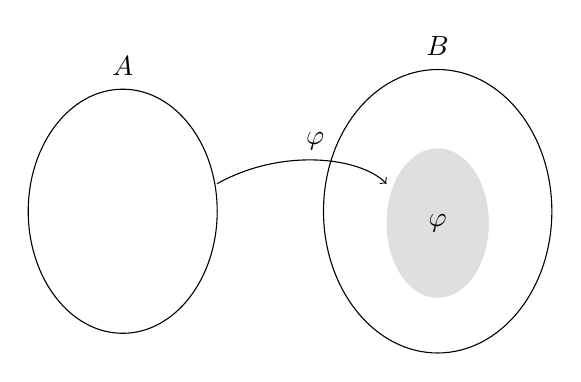
\begin{tikzpicture}[x=1cm,y=1cm,baseline=(current bounding box.center)]
\draw (-2,0) ellipse (1.2 and 1.55) node[above=1.6cm] {$A$};
\draw (2,0) ellipse (1.45 and 1.8) node[above=1.85cm] {$B$};
\fill[gray!25] (2,-.15) ellipse (.65 and .95);
\node at (2,-.15) {$\Image\varphi$};
\draw[->] (-.8,.35) .. controls (0,.8) and (1,.7) .. (1.35,.35) node[midway,above] {$\varphi$};
\end{tikzpicture}
\end{center}
\indent 我们可以把许多``子对象''塞进 $B$, 使得 $A$ 通过 $\varphi$ 映到它们:
\begin{center}
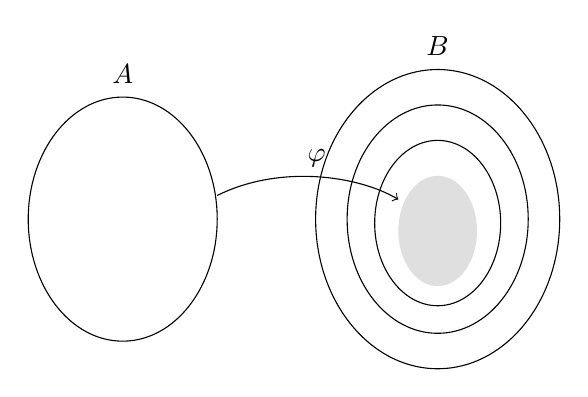
\begin{tikzpicture}[x=1cm,y=1cm,baseline=(current bounding box.center)]
\draw (-2,0) ellipse (1.2 and 1.55) node[above=1.6cm] {$A$};
\draw (2,0) ellipse (1.55 and 1.9) node[above=1.95cm] {$B$};
\draw (2,0) ellipse (1.15 and 1.45);
\draw (2,-.05) ellipse (.8 and 1.05);
\fill[gray!25] (2,-.15) ellipse (.5 and .7);
\draw[->] (-.8,.3) .. controls (0,.7) and (1,.55) .. (1.5,.25) node[midway,above] {$\varphi$};
\end{tikzpicture}
\end{center}
而 $\Image\varphi$ 是``最小的''这样的子对象; 也就是说, 它是初始的, 具有作为 $B$ 的一个子对象、且 $\varphi$ 经过它分解的性质. 一旦我们习惯于把``子对象''想成``单态射'', 这一直觉就被 $\Ker(\Coker\varphi)$ 精确地捕捉到了:

\begin{lemma}\label{lem:image-universal}
设 $\varphi:A\to B$ 是 Abel 范畴中的一个态射, 并设 $i:K\to B$ 是 $\varphi$ 的余核的核. 那么
\begin{itemize}
\item $i$ 是一个单态射;
\item $\varphi$ 经过 $i$ 分解; 并且
\item $i$ 在具有这些性质的意义上是初始的.
\end{itemize}
\end{lemma}

\indent 由引理~\ref{lem:kernels-mono-cokernels-epi}, $i$ 是单态射. 显然 $\varphi$ 经过 $i$ 分解: 复合 $A\to B\to\Coker\varphi$ 是零态射, 所以由核的泛性质自然诱导出一个 $A\to K$. 引理~\ref{lem:image-universal} 陈述中更有趣的部分是: 如果 $\lambda:L\hookrightarrow B$ 是任何一个 $\varphi$ 也经过它分解的单态射, 那么 $i$ 必须唯一地经过 $\lambda$ 分解:
\begin{center}
\begin{tikzcd}[column sep=large,row sep=large]
& L \ar[dr,hook,"\lambda"] & \\
A \ar[ur] \ar[r] & K \ar[u,dashed,"\exists!"] \ar[r,hook,"i"'] & B
\end{tikzcd}
\end{center}

\begin{proof}
考虑 $\Coker\lambda$:
\begin{center}
\begin{tikzcd}[column sep=large,row sep=large]
& L \ar[dr,hook,"\lambda"] & \\
A \ar[ur] \ar[r] & K \ar[r,hook,"i"'] & B \ar[r,"\Coker\lambda"] & \Coker\lambda
\end{tikzcd}
\end{center}
由于 $\varphi$ 经过 $\lambda$ 分解, 复合 $A\to B\to C$ 是 $0$; 由 $\Coker\varphi$ 的泛性质, 我们有一个诱导映射:
\begin{center}
\begin{tikzcd}[column sep=large,row sep=large]
& L \ar[dr,hook,"\lambda"] & & \\
A \ar[ur] \ar[r,"\varphi"'] & K \ar[r,hook,"i"'] & B \ar[r,"\Coker\varphi"] \ar[dr,"\Coker\lambda"'] & \Coker\varphi \ar[d,dashed,"\exists!"] \\
& & & \Coker\lambda
\end{tikzcd}
\end{center}
由于 $K\to\Coker\varphi$ 是零态射, 上图推出复合
\[
K\longrightarrow B\longrightarrow\Coker\lambda
\]
是零态射. 因为 $\lambda:L\to B$ 是它的余核的核 (引理~\ref{lem:kernel-of-cokernel}), 由此存在一个唯一的态射 $K\to L$ 使图表交换, 如断言.
\end{proof}

\begin{definition}\label{def:image-coimage}
设 $\varphi:A\to B$ 是 Abel 范畴中的一个态射. $\varphi$ 的\emph{象} (image), 记作 $\Image\varphi$, 是 $\Ker(\Coker\varphi)$. $\varphi$ 的\emph{余象} (coimage), 记作 $\Coim\varphi$, 是 $\Coker(\Ker\varphi)$.
\end{definition}

\indent 引理~\ref{lem:image-universal} 启发了第一个定义: 每个 $\varphi$ 经过它分解的单态射都必须唯一地经过 $\Image\varphi$ 分解. (当然在这个语境中 $\Image\varphi$ 的源只定义到 (唯一) 同构, 正如每个泛问题的解一样.) 至于第二个定义, 读者将表述 $\Coim\varphi$ 满足的泛性质 (习题~\ref{ex:1.19}). 利用注记~\ref{rmk:epi-quotient} 中提到的约定并允许某种语言的滥用, $\varphi:A\to B$ 的余象 (的靶) 是``商'' $A/\Ker\varphi$.
我们的心目所想, 当然还有你们的, 都提示说: 如果 $K\hookrightarrow B$ 是 $\varphi$ 的象, 那么诱导出的态射 $\widetilde{\varphi}:A\to K$,
\begin{center}
\begin{tikzcd}
A \ar[r, "\widetilde{\varphi}"] \ar[dr, "\varphi"'] & K \ar[d, "i"] \\
& B
\end{tikzcd}
\end{center}
应当是一个满态射. 情况的确如此:

\begin{lemma}\label{lem:coimage-image-epi-mono}
设 $\varphi:A\to B$ 是 Abel 范畴中的一个态射, 并设 $\Image\varphi:K\hookrightarrow B$, $\Coim\varphi:A\to C$ 分别是它的象与余象. 那么诱导出的态射 $A\to K$ 与 $C\to B$ 分别是满态射与单态射.
\end{lemma}

\begin{proof}
像通常一样, 我们将证明陈述的一半, 把另一半留给读者 (习题~\ref{ex:1.20}).
要验证 $\widetilde{\varphi}:A\to K$ 是满态射, 考虑它的象 $K'\hookrightarrow K$:
\begin{center}
\begin{tikzcd}[column sep=large]
K' \ar[r,hook,"\Image\widetilde\varphi"] & K \ar[r,"\Coker\widetilde\varphi"] & \Coker\widetilde\varphi
\end{tikzcd}
\end{center}
回忆每个满态射都是它的核的余核 (引理~\ref{lem:kernel-of-cokernel}); 特别地, $\Coker\widetilde{\varphi}=\Coker(\Image\varphi)$. 现在, $K'\hookrightarrow K$ 是一个 $\widetilde{\varphi}$ 经过它分解的单态射:
\begin{center}
\begin{tikzcd}[column sep=large,row sep=large]
A \ar[r,two heads,"\widetilde\varphi"] \ar[rr,bend right=22,"\varphi"'] & K' \ar[r,hook] & K \ar[r,hook,"\Image\varphi"] & B
\end{tikzcd}
\end{center}
因此 $K'\hookrightarrow B$ 是一个 $\varphi$ 经过它分解、并且``先于'' $\Image\varphi:K\hookrightarrow B$ 的单态射. 因为 $\varphi$ 的象在那样的态射中是初始的 (如引理~\ref{lem:image-universal} 所证), 必然有 $\Image\widetilde{\varphi}$ 是一个同构. 由此推出 $0=\Coker(\Image\widetilde{\varphi})=\Coker\widetilde\varphi$, 从而由引理~\ref{lem:kernel-zero-mono} 证明 $\widetilde{\varphi}$ 是满态射.
\end{proof}

\indent 总结一下形势, 我们有如下交换图表, 由满态射与单态射分解一个给定的 Abel 范畴中的态射 $\varphi$:
\begin{center}
\begin{tikzcd}[column sep=large,row sep=large]
A \ar[r,two heads,"\Coim\varphi"] \ar[rrr,bend right=22,"\varphi"'] & C \ar[r,"\widetilde\varphi"] & K \ar[r,hook,"\Image\varphi"] & B
\end{tikzcd}
\end{center}
\indent 希望我们没有迷失我们所追寻的``标准分解'':
\[
A\xrightarrow{\Coim\varphi} C\xrightarrow{\widetilde{\varphi}} K\xrightarrow{\Image\varphi} B.
\]
我们现在看到, 这等于如下陈述: 在 Abel 范畴中, 存在一个诱导的同构联系起每个态射的余象与象.
\begin{proof}[定理~\ref{thm:canonical-decomposition-morphism} 的证明]
由 $\Image\varphi$ 的泛性质 (引理~\ref{lem:image-universal}) 以及 $\Coim\varphi$ 的泛性质, 存在唯一的态射 $\psi:K\to C$ 使上图交换. 记诱导的态射 $A\to K$ 为 $\bar\varphi$, 记诱导的态射 $C\to B$ 为 $\hat\varphi$. 由于 $\hat\varphi\circ\psi=\Image\varphi$ 是单态射, $\psi$ 也是单态射; 由于 $\psi\circ\bar\varphi=\Coim\varphi$ 是满态射, $\psi$ 也是满态射. 因而 $\psi$ 是同构 (引理~\ref{lem:mono-epi-iso}), 取 $\widetilde\varphi:C\to K$ 为它的逆即完成证明.
\end{proof}
\indent 粗略地说, 我们可以说, 在 Abel 范畴中,``象与余象自然同构''. 这不精确, 因为象与余象本身是态射; 同构存在于余象的靶与象的源之间. 当然, 对于像 $R\dcate{-Mod}$ 这样友好的范畴, 这一区别无关紧要.

\subsection*{习题}
\phantomsection
\addcontentsline{toc}{subsection}{习题}

\begin{prob}\label{ex:1.1}
证明: 如果 $\psi\circ\varphi$ 是满态射, 那么 $\psi$ 是满态射. 证明: 如果 $\psi\circ\varphi$ 是单态射, 那么 $\varphi$ 是单态射.
\end{prob}

\begin{prob}\label{ex:1.2}
设 $\varphi:A\to B$ 是加性范畴中的一个态射. 证明 $-\varphi$ 是单态射 (相应地, 满态射) 当且仅当 $\varphi$ 是.
\end{prob}

\begin{prob}\label{ex:1.3}
一个\emph{预加性范畴} (preadditive category) 是指每个 Hom 集都被赋予一个 Abel 群结构、且使得复合映射是双线性的范畴. 证明: 一个环``等同于''一个只有一个对象的预加性范畴. 加性范畴就是带有零对象与有限积、有限余积的预加性范畴. 注意``预加性范畴之间的加性函子''这一概念是有意义的. [习题~\ref{ex:1.12}]
\end{prob}

\begin{prob}\label{ex:1.4}
设 $\mathcal{A}$ 是一个加性范畴 (预加性即足够), 并设 $A$ 是 $\mathcal{A}$ 的一个对象. 证明 $\End_{\mathcal{A}}(A)$ 有一个自然的环结构.
\end{prob}

\begin{prob}\label{ex:1.5}
设 $A,B$ 是加性范畴 $\mathcal{A}$ 的对象, 零对象为 $0$. 由于 $0$ 既是终对象也是始对象, $\Hom_{\mathcal{A}}(A,0)$ 与 $\Hom_{\mathcal{A}}(0,B)$ 都是单点集, 所以复合
\[
A\longrightarrow 0\longrightarrow B
\]
的象是 $\Hom_{\mathcal{A}}(A,B)$ 中的单个元素 $e$. 证明这是 Abel 群 $\Hom_{\mathcal{A}}(A,B)$ 的单位元. (提示: 证明 $e+e=e$.) 在正文里这个元素记作 $0$, 即``零态射''. 证明对每个态射 $\varphi$, 有 $\varphi\circ 0=0\circ\varphi=0$.
\end{prob}

\begin{prob}\label{ex:1.6}
证明: 对象 $A$ 是零对象当且仅当 $\id_A$ 等于零态射 $A\to A$. [\S\ref{subsec:4.2-quasi-iso-derived}]
\end{prob}

\begin{prob}\label{ex:1.7}
\index{fanchoulundingyi@范畴论定义(categorical definition)!mo@模(module)!zhuanzhi@转置(transpose)}\index{fanchoulundingyi@范畴论定义(categorical definition)!moqun@模群(modular group)!zhuanzhi@转置(transpose)}\index{fanchoulundingyi@范畴论定义(categorical definition)!Möbius bianhuan@Möbius 变换(Möbius transformation)!zhuanzhi@转置(transpose)}\index{fanchoulundingyi@范畴论定义(categorical definition)!juzhendezishi@矩阵的子式(minor of a matrix)!zhuanzhi@转置(transpose)}\index{fanchoulundingyi@范畴论定义(categorical definition)!jixiaoduoxiangshi@极小多项式(minimal polynomial)!zhuanzhi@转置(transpose)}\index{fanchoulundingyi@范畴论定义(categorical definition)!Milne@Milne!James S.@James S.!zhuanzhi@转置(transpose)}\index{fanchoulundingyi@范畴论定义(categorical definition)!McKay@McKay!James@James!zhuanzhi@转置(transpose)}\index{fanchoulundingyi@范畴论定义(categorical definition)!jidalixiang@极大理想(maximal ideal)!zhuanzhi@转置(transpose)}\index{fanchoulundingyi@范畴论定义(categorical definition)!zhuanzhi@转置(transpose)}\index{fanchoulundingyi@范畴论定义(categorical definition)!dehuan@的环(of a ring)}\index{fanchoulundingyi@范畴论定义(categorical definition)!deyoulidianfanxingshi@的有理典范形式(rational canonical form of)}\index{fanchoulundingyi@范畴论定义(categorical definition)}仿照例~VIII.\ref{ex:equalizers-kernels} 中对核给出的范畴论定义, 给出余核的一个范畴论定义, 并验证 $R\dcate{-Mod}$ 中通常的余核概念满足这一范畴论要求. 验证你的定义与定义~\ref{def:kernel-cokernel} 给出的定义一致.
\end{prob}

\begin{prob}\label{ex:1.8}
设 $\varphi:A\to B$ 是加性范畴 $\mathcal{A}$ 中的一个态射. 证明 $i:K\to A$ 是 $\varphi$ 的核, 当且仅当对所有的对象 $Z$, 诱导出的序列
\[
0\longrightarrow\Hom_{\mathcal{A}}(Z,K)\longrightarrow\Hom_{\mathcal{A}}(Z,A)\longrightarrow\Hom_{\mathcal{A}}(Z,B)
\]
是正合的. 对余核表述一个类似的结果.
\end{prob}

\begin{prob}\label{ex:1.9}
这个练习完成正文中给出的结果的证明. 这些论证应当构造得能镜像正文中所引述的引理的配对陈述的证明.
设 $\mathcal{A}$ 是一个加性范畴.
\begin{itemize}
\item 设 $i:K\to A$ 是 $\mathcal{A}$ 中的一个核; 证明 $i$ 是单态射. (Cf. 引理~\ref{lem:kernels-mono-cokernels-epi}.)
\item 设 $\varphi:A\to B$ 是 $\mathcal{A}$ 中的一个态射. 如果 $\varphi$ 有余核, 证明 $\varphi$ 是满态射当且仅当 $B\to 0$ 是它的余核. (Cf. 引理~\ref{lem:kernel-zero-mono}.)
\item 如果 $\mathcal{A}$ 是 Abel 的, 证明 $\mathcal{A}$ 中的每个核都是它的余核的核. (Cf. 引理~\ref{lem:kernel-of-cokernel}.)
\end{itemize}
[\S\ref{subsec:abelian-categories}]
\end{prob}

\begin{prob}\label{ex:1.10}
证明 Abel 范畴的对立范畴 $\mathcal{A}\op$ (cf. 习题~I.\ref{ex:opposite-category}) 是一个 Abel 范畴. [\S\ref{subsec:5.3-proj-inj}]
\end{prob}

\begin{prob}\label{ex:1.11}
设 $\mathcal{A}$ 是一个 Abel 范畴, 并设 $C$ 是任意小的范畴. 证明函子范畴 $\mathcal{A}^C$ (cf. 习题~VIII.\ref{ex:functor-category}) 是一个 Abel 范畴.
对 $C$ 的每个对象 $X$, 证明赋值 $\mathcal{F}\mapsto\mathcal{F}(X)$ (对 $\mathcal{A}^C$ 中态射的作用显而易见, 即自然变换) 决定一个正合函子 $\mathcal{A}^C\to\mathcal{A}$. [习题~\ref{ex:1.12}, \ref{ex:1.14}, \ref{ex:1.15}, 习题~\ref{ex:2.15}, 习题~\ref{ex:5.7}]
\end{prob}

\begin{prob}\label{ex:1.12}
对环 $R$, 令 $\underline{R}$ 表示由 $R$ 决定的只有一个对象的预加性范畴 (习题~\ref{ex:1.3}). 证明左 $R$-模范畴 $R\dcate{-Mod}$ 等价于由加性函子构成的函子范畴 $\cate{Ab}^{\underline{R}}$ 的全子范畴 (cf. 习题~\ref{ex:1.11}). 右 $R$-模的范畴又如何?
\end{prob}

\begin{prob}\label{ex:1.13}
设 $R$ 是一个交换环, 并设 $R\dcate{-Mod}_f$ 表示有限生成 $R$-模的范畴. 说明 $R\dcate{-Mod}_f$ 不必是一个 Abel 范畴; 证明只要 $R$ 是 Noether 的, 它就是.
\end{prob}

\begin{prob}\label{ex:1.14}
设 $T$ 是一个拓扑空间. 回忆 $T$ 上取值于范畴 $\mathcal{A}$ 的\emph{预层} (presheaf) 是一个由与 $T$ 相关联的某个范畴到 $\mathcal{A}$ 的反变函子 (例~VIII.\ref{ex:presheaf-set}). 定义 $T$ 上取值于 $\mathcal{A}$ 的\emph{预层} (presheaf) 的范畴. 证明取值于 Abel 范畴的 $T$ 上的预层构成一个 Abel 范畴. (提示: 习题~\ref{ex:1.11}.)
\end{prob}

\begin{prob}\label{ex:1.15}
考虑圆 $S^1$ 上连续复值函数预层 $\mathcal{F}$ (cf. 习题~VIII.\ref{ex:presheaf-ab-groups}) 与沿圆周处处不为零的连续复值函数预层 $\mathcal{F}^*$; 第一个是 (在 $+$ 下) Abel 群的层, 第二个也是 (在 $\cdot$ 下). 用指数映射定义一个态射 $\exp:\mathcal{F}\to\mathcal{F}^*$.
证明 $\exp$ 不是预层的一个满态射\footnote{注意! 两个预层 $\mathcal{F},\mathcal{F}^*$ 都满足层条件; cf. 习题~VIII.\ref{ex:presheaf-ab-groups}. Abel 群的层构成预层范畴的一个全子范畴, 并且这个范畴也是 Abel 的, 但是包含函子一般不是正合的. 例如, 上面考虑的的指数映射 $\mathcal{F}\to\mathcal{F}^*$ 是一个层的满态射. 此外, 对 $T$ 的每个开集 $U$, 赋值 $\mathcal{F}\mapsto\mathcal{F}(U)$ 同时在 Abel 群预层范畴与 Abel 群层范畴上定义一个函子. 这个函子在预层上是正合的 (这是习题~\ref{ex:1.11} 的一个特例), 但上面给出的例子表明它在层上一般不是正合的. 这种正合性的缺失正是层上同调存在的原因.}: 证明它的余核在 $S^1$ 的每个真开集上取值为 $0$, 却在 $S^1$ 上非零.
\end{prob}

\begin{prob}\label{ex:1.16}
考虑 Abel 范畴中的一个拉回图表
\begin{center}
\begin{tikzcd}[column sep=large,row sep=large]
A\times_C B \ar[r,"\varphi'"] \ar[d,"\psi'"'] & B \ar[d,"\psi"] \\
A \ar[r,"\varphi"'] & C
\end{tikzcd}
\end{center}
证明从 $\Ker\varphi'$ 的源到 $\Ker\varphi$ 的源诱导出的态射是一个同构.
对推出陈述并证明一个类似的结果. [\S\ref{subsec:products-coproducts}, \S\ref{subsec:snake-lemma-again}, \S\ref{subsec:6.2-objects-complexes}]
\end{prob}

\begin{prob}\label{ex:1.17}
证明对 Abel 范畴的对象 $A,B$ 定义的态射 $A\amalg B\to A\times B$ 是一个满态射. [\S\ref{subsec:products-coproducts}]
\end{prob}

\begin{prob}\label{ex:1.18}
在 Abel 范畴中, 对两个有共同靶 $Z$ 的单态射 $A\hookrightarrow Z$, $B\hookrightarrow Z$, 表述``交'' (intersection) 的概念. 证明自然单态射 $A\hookrightarrow A\oplus B$, $B\hookrightarrow A\oplus B$ 的交是 $0$.
\end{prob}

\begin{prob}\label{ex:1.19}
表述 Abel 范畴中一个态射的余象满足的泛性质. [\S\ref{subsec:images-canonical-decomposition}]
\end{prob}

\begin{prob}\label{ex:1.20}
设 $A\to B$ 是 Abel 范畴中的一个态射, 余象为 $A\to C$, 并设 $C\to B$ 是诱导出的态射. 证明 $C\to B$ 是一个单态射. (Cf. 引理~\ref{lem:coimage-image-epi-mono}; 你不应使用定理~\ref{thm:canonical-decomposition-morphism}, 因为引理~\ref{lem:coimage-image-epi-mono} 在其证明中被用到.) [\S\ref{subsec:images-canonical-decomposition}]
\end{prob}

\begin{prob}\label{ex:1.21}
设 $\varphi:A\to B$ 是 Abel 范畴中的一个态射, 并假设 $\varphi$ 分解为一个满态射 $\pi$ 接着一个单态射 $i$:
\[
\begin{tikzcd}[ampersand replacement=\&,column sep=large]
A \ar[r,two heads,"\pi"] \ar[rr,bend right=24,"\varphi"'] \& C \ar[r,hook,"i"] \& B
\end{tikzcd}
\]
证明必然有 $\pi=\Coim\varphi$ 且 $i=\Image\varphi$. [\S\ref{subsec:7.4-les}]
\end{prob}

\begin{prob}\label{ex:1.22}
$\vartriangleright$\ 证明任意加性范畴中的有限积与有限余积重合. (提示: 为证明 $A\amalg B$ 满足 $A\times B$ 的泛性质, 给定态射 $\alpha:C\to A$ 与 $\beta:C\to B$, 用 $i_A\circ\alpha+i_B\circ\beta$ 定义 $C\to A\amalg B$.) [\S\ref{subsec:products-coproducts}]
\end{prob}

\section{在 Abel 范畴中工作}
\label{sec:working-abelian-categories}

\subsection{Abel 范畴中的正合性}
\label{subsec:exactness-abelian}

\index{zhenghe@正合(exact)}既然我们在任一 Abel 范畴中都有了``象''的良好概念, 我们就可以形式化``正合列'' (exact sequence) 的含义. 考虑 Abel 范畴中一列对象与态射
\[
\cdots \longrightarrow A \xrightarrow{\varphi} B \xrightarrow{\psi} C \longrightarrow \cdots
\]
该列在 $B$ 处\emph{正合} (exact), 如果
\begin{enumerate}
\item[(1)] $\psi\circ\varphi=0$, 并且
\item[(2)] $\Coker\varphi\circ\ker\psi=0$.
\end{enumerate}
第一个条件使得该列成为一个``复形'' (complex); 它告诉我们 $\varphi$ 经过 $\ker\psi$ 分解. 由于 $\ker\psi$ 是单态射, 象的泛性质 (引理~\ref{lem:image-universal}) 给出 $\Image\varphi$ 经过 $\ker\psi$ 的唯一分解. 类似地, 第二个条件告诉我们 $\ker\psi$ 经过 $\ker(\Coker\varphi)=\Image\varphi$ 分解. 这意味着 $\Image\varphi$ 与 $\ker\psi$ 重合. 因此, 定义正合性的条件可以概括为
\[
\Image\varphi=\ker\psi.
\]
当然, 这精确地重新得到了我们在 §III.\ref{subsec:complexes} 中用来定义 $R$-模之列的正合性时所用的条件.
正如我们在 \S\ref{subsec:additive-categories}--\S\ref{subsec:abelian-categories} 中已经预见的那样, 正合性所有预期的初等同义表述在 Abel 范畴的语境下都如同在 $R\dcate{-Mod}$ 中一样成立. 沿用上面的记号, 如果该列在 $B$ 处正合, 那么
\begin{itemize}
\item $\psi$ 是单态射, 当且仅当 $\varphi$ 是零态射;
\item $\varphi$ 是满态射, 当且仅当 $\psi$ 是零态射;
\end{itemize}
并且该列
\[
0\to A\xrightarrow{\varphi} B\xrightarrow{\psi} C\to 0
\]
正合, 当且仅当 $\varphi$ 是 $\psi$ 的核且 $\psi$ 是 $\varphi$ 的余核; 而该列
\[
0\to A\xrightarrow{\varphi} B\to 0
\]
正合, 当且仅当 $\varphi$ 是同构.

\begin{example}\label{ex:exact-seq-direct-sum}
存在一个自然的正合列
\[
0\to A\to A\oplus B\to B\to 0,
\]
其中 $A\oplus B$ 是 \S\ref{subsec:products-coproducts} 中定义的直和.
\end{example}

\begin{example}\label{ex:pullback-sequence}
作为一个略微更有趣的例子, 考虑如下图表
\begin{center}
\begin{tikzcd}
& B \ar[dr, "\psi"] & \\
D \ar[ur, "\alpha'"] \ar[dr, "\alpha"'] & & C \\
& A \ar[ur, "\varphi"']
\end{tikzcd}
\end{center}
以及由它得到的列
\[
D \xrightarrow{(\alpha,\alpha')} A\oplus B \xrightarrow{(\varphi,-\psi)} C,
\]
这里让 $A\oplus B$ 同时扮演积与余积两个角色 (即把 $D\to A$, $D\to B$ 分别映为 $A\oplus B$ 的两个分量). 于是
\begin{itemize}
\item 该图表交换, 当且仅当这一列是一个复形;
\item 在左边添上 $0$ 得到的列
\[
0\to D\to A\oplus B\to C
\]
正合, 当且仅当 $D$ 可等同于纤维积 $A\times_C B$ (cf. 例~\ref{ex:fibered-products-abelian});
\item 类似地, 该列
\[
D\to A\oplus B\to C\to 0
\]
正合, 当且仅当 $C$ 可等同于纤维余积 $A\amalg_D B$.
\end{itemize}
\end{example}
\indent 事实上, 第一个断言是平凡的; 第二个与第三个断言归结为例~\ref{ex:fibered-products-abelian} 中提到的纤维积与纤维余积的显式构造.\erratumfootnote{官方勘误图主张补入``纤维余积时结论相差一个同构、须计入交换余积的符号''这一说明；第二次印刷正文无此补充，故此处从第二次印刷。}

\subsection{蛇引理, 重访}
\label{subsec:snake-lemma-again}

读者现在已能在任一 Abel 范畴中理解 §III.\ref{subsec:complexes-homology} 为 $R$-模之列给出的所有陈述; 这包括把一个复形的同调定义为正合性失败的一种度量. 这些事实将在 \S\ref{sec:complexes-homology-again} 中回顾. 然而请注意, 虽然我们现在能在任一 Abel 范畴中陈述蛇引理 (引理~III.\ref{lem:snake}), 但 §III.\ref{subsec:complexes-homology} 中给出的 (证明的轮廓) 并不能直接从那个语境搬过来套用到这个语境上, 至少乍看之下如此, 因为 §III.\ref{subsec:complexes-homology} 中给出的``连接''同态 $\delta$ 的定义用到了``元素''. 抛开更精巧的替代方案不谈, 我们应当为 $\delta$ 的定义提供一个箭头论的替代.
这或许并不是完全轻而易举的.
作为练习, 注意以下事实:

\begin{lemma}\label{lem:pullback-epi}
设
\begin{center}
\begin{tikzcd}[column sep=large,row sep=large]
A\times_C B \ar[r,two heads,"\varphi'"] \ar[d,"\psi'"'] & B \ar[d,"\psi"] \\
A \ar[r,two heads,"\varphi"'] & C
\end{tikzcd}
\end{center}
是 Abel 范畴中的一个纤维方形, 并设 $\varphi$ 是满态射. 那么 $\varphi'$ 也是满态射.
\end{lemma}

\indent 用元素追踪, 几秒钟就能发现这在 $R\dcate{-Mod}$ 中成立. 一个箭头论的证明则要微妙得多.

\begin{proof}
首先, 观察到若 $\varphi:A\to C$ 是满态射, 则例~\ref{ex:pullback-sequence} 中考虑的映射 $A\oplus B\to C$ 也是满态射. 由于在 Abel 范畴中满态射就是余核, 而余核又是其核的余核 (引理~\ref{lem:kernel-of-cokernel}), 我们看到 $A\oplus B\to C$ 是自然的态射
\[
A\times_C B\to A\oplus B
\]
的余核.
要证明 $\varphi'$ 是满态射, 只需 (引理~\ref{lem:mono-epi-additive}) 证明: 对任何满足 $\gamma\circ\varphi'=0$ 的态射 $\gamma:B\to Z$, 都有 $\gamma=0$.
为此, 考虑由 $A\oplus B$ 是 $A$ 与 $B$ 的余积这一事实得到的态射
\[
A\oplus B\to Z.
\]
其复合
\[
A\times_C B\to A\oplus B\to Z
\]
与 $\gamma\circ\varphi'$ 一致, 因而为零态射. 
\[
\begin{tikzcd}[ampersand replacement=\&,column sep=large,row sep=large]
A\oplus B \ar[r,"(0{,}\gamma)"] \ar[d] \& Z \\
C \ar[ur,dashed,"\gamma'"'] \&
\end{tikzcd}
\]
由余核的泛性质, 我们得到一个唯一的分解态射; 由图表的交换性
\[
\begin{tikzcd}[ampersand replacement=\&,column sep=large,row sep=large]
A \ar[r] \ar[dr,"\varphi"'] \& A\oplus B \ar[r,"(0{,}\gamma)"] \ar[d] \& Z \\
\& C \ar[ur,"\gamma'"'] \&
\end{tikzcd}
\]
可见, 该态射与 $\gamma'\circ\varphi:A\to C\to Z$ 的复合为零态射. 由于 $\varphi$ 是满态射, 由此推出该态射为 $0$. 这意味着 $(0,\gamma):A\oplus B\to Z$ 为零态射, 于是我们证毕: $\gamma=0$, 正如所断言.
\end{proof}

\indent 这里有一个更快的证明 (给那些做了作业的人): 若 $\varphi$ 是满态射, 则 $A\oplus B\to C$ 是满态射, 因此该图表既是推出又是拉回 (例~\ref{ex:pullback-sequence}). 由习题~\ref{ex:1.16}, $\Coker\varphi'=\Coker\varphi=0$; 因此 $\varphi'$ 是满态射. 读者现在应当毫不费力地证明引理~\ref{lem:pullback-epi} 的对偶陈述, 即关于纤维余积的情形 (习题~\ref{ex:2.2}).
回到蛇引理, 从一个连结两个 Abel 范畴中正合列的交换图表出发:
\begin{center}
\begin{tikzcd}[column sep=large,row sep=large]
0 \ar[r] & L_1 \ar[r,"\alpha_1"] \ar[d,"\lambda"] & M_1 \ar[r,"\beta_1"] \ar[d,"\mu"] & N_1 \ar[r] \ar[d,"\nu"] & 0 \\
0 \ar[r] & L_0 \ar[r,"\alpha_0"'] & M_0 \ar[r,"\beta_0"'] & N_0 \ar[r] & 0
\end{tikzcd}
\end{center}
主要任务是构造一个连接同态\footnote{为避免难以承受的繁复记号, 我们将把 $\ker\nu$, 等等, 简写为相应态射的源, 即把 $\ker\nu$ 记作态射 $\ker\nu\to N_1$ 的源, 等等.} $\delta:\ker\nu\to\Coker\lambda$; 一旦做到这一点, 我们就应当证明引理~III.\ref{lem:snake} 中显示的那一列的正合性. 我们将把这后一步留给更有闯劲的读者 (他或许愿意等到我们过完 \S\ref{subsec:working-with-elements} 再做).
有闯劲的读者其实应该亲自尝试构造 $\delta$, 把它当作一个用箭头论证明替换耳熟能详的元素论论证的练习. 尽可在此停笔, 自己试过之后再继续往下读.
``问题''在于: 核与余核的泛性质似乎只保证存在到 $\ker\nu$ 的态射与从 $\Coker\lambda$ 出发的态射. 症结正在于此: 我们到底怎样才能得到一个从 $\ker\nu$ 到 $\Coker\lambda$ 的态射? (最后一次自己尝试的机会!)
\indent 答案是把 $\ker\nu$ 看成一个余核, 把 $\Coker\lambda$ 看成一个核. 这可以通过构造合适的拉回 (相应地, 推出) 图表来实现:
\begin{center}
\begin{tikzcd}[column sep=large,row sep=large]
M_1\times_{N_1}(\ker\nu) \ar[r,two heads,"\beta'_1"] \ar[d] & \ker\nu \ar[d] \\
M_1 \ar[r,two heads,"\beta_1"'] & N_1
\end{tikzcd}
\qquad\qquad
\begin{tikzcd}[column sep=large,row sep=large]
L_0 \ar[r,"\alpha_0"] \ar[d] & M_0 \ar[d] \\
\Coker\lambda \ar[r,hook,"\alpha'_0"'] & \Coker\lambda\amalg_{L_0}M_0
\end{tikzcd}
\end{center}
由引理~\ref{lem:pullback-epi}, 由于 $\beta_1:M_1\to N_1$ 是满态射, 左图中的 $\beta'_1:M_1\times_{N_1}(\ker\nu)\to\ker\nu$ 也是满态射; 并且由习题~\ref{ex:1.16}, $\ker\beta_1$ 与 $\ker\beta'_1$ 有匹配的源. 对第二个图表也有类似 (对偶) 的陈述 (习题~\ref{ex:2.2} 与习题~\ref{ex:1.16}). 把一切都放进一个交换图表, 我们得到
\begin{center}
\begin{tikzcd}[column sep=1.35em,row sep=1.7em,font=\small]
0 \ar[r] & L_1 \ar[r,"\sigma"] \ar[d,equal] & M_1\times_{N_1}(\ker\nu) \ar[r,two heads,"\beta'_1"] \ar[d] \ar[ddd,bend right=18,"\varepsilon"'] & \ker\nu \ar[r] \ar[d] & 0 \\
0 \ar[r] & L_1 \ar[r,"\alpha_1"] \ar[d,"\lambda"'] & M_1 \ar[r,"\beta_1"] \ar[d,"\mu"] & N_1 \ar[r] \ar[d,"\nu"] & 0 \\
0 \ar[r] & L_0 \ar[r,"\alpha_0"] \ar[d] & M_0 \ar[r,"\beta_0"] \ar[d] & N_0 \ar[r] \ar[d,equal] & 0 \\
0 \ar[r] & \Coker\lambda \ar[r] & \Coker\lambda\amalg_{L_0}M_0 \ar[r,"\tau"] & N_0 \ar[r] & 0
\end{tikzcd}
\end{center}
一个行正合 (而非列正合!) 的图表. 由此得到一个态射
\[
\varepsilon: M_1\times_{N_1}(\ker\nu)\to \Coker\lambda\amalg_{L_0}M_0.
\]
注意
\[
\varepsilon\circ\sigma=0,\qquad \tau\circ\varepsilon=0
\]
(由图表的交换性): 事实上, 复合
\[
L_1\to\Coker\lambda,\qquad \ker\nu\to N_0
\]
都为零. 由于 $\ker\nu$ 在顶行中扮演余核的角色, $\varepsilon\circ\sigma=0$ 意味着 $\varepsilon$ 经过 $\ker\nu$ 分解, 给出一个态射
\[
\varepsilon':\ker\nu\to \Coker\lambda\amalg_{L_0}M_0.
\]
由于 $\Coker\lambda$ 在底行中扮演核的角色, 而 $\tau\circ\varepsilon':\ker\nu\to N_0$ 为零态射 (因为 $(\tau\circ\varepsilon')\circ\beta'_1=\tau\circ\varepsilon=0$, 且 $\beta'_1$ 是满态射), $\varepsilon'$ 必须再经过 $\Coker\lambda$ 分解, 最终给出
\[
\delta:\ker\nu\to\Coker\lambda.
\]
把元素写出来, 读者可以验证这个态射 $\delta$ 与 §III.\ref{subsec:snake-lemma} 中定义的连接同态 $\partial$ 一致. 连同由更简单的考虑诱导出的映射一起, 我们在 Abel 范畴中得到如下一列态射
\[
0\to\ker\lambda\to\ker\mu\to\ker\nu\xrightarrow{\delta}\Coker\lambda\to\Coker\mu\to\Coker\nu\to 0.
\]
我们现在应当建议读者用适当的箭头论论证来证明这一列的正合性. 这为我们最终开始发展同调代数时将遇到的许多此类事实提供了绝佳的练习.
然而, 假设我们已在 §III.\ref{subsec:snake-lemma} 中用元素追踪做完了这件工作, 为了核查该列在 Abel 范畴中的正合性, 真的有必要回过头用箭头重做一遍吗?

\subsection{在小的 Abel 范畴中用``元素''工作}
\label{subsec:working-with-elements}

我们个人的感觉是, 箭头论论证 总是 比它们对应的元素论论证更有洞察力, 即便它们照例``更难''. 至少, 它们更优雅: 例如, 在上面给出的连接同态 $\delta$ 的构造中, 无需验证结果是否``良定义'', 而在 §III.\ref{subsec:snake-lemma} 的集合论构造中这需要一番论证. 这类问题通常在开头一旦确立了关键的泛性质就被一劳永逸地解决了, 无需在后面反复啰嗦.
尽管如此, 元素论论证通常确实更容易想出来. 引理~\ref{lem:pullback-epi} 似乎就是一个好例子: 用元素的语言, 这个引理的陈述完全显然, 从图表的观点看却没那么显然. 习题~\ref{ex:2.12} 给出了另一个例子: 为那里陈述一个人畜无害的结果提供一个纯箭头论的证明并不容易, 而从更平凡的观点看它几乎是显然的. 读者或许会疑惑, 对于核查一个图表的交换性或一列的正合性这类事实, 仅仅用更简单的元素论考虑去证明是否``足够''.
情况确实如此. 我们将给出一个构造, 它足以 (例如) 通过追踪元素而非箭头来完成蛇引理的证明. 我们发现这个构造既有教益又漂亮, 因此愿花些时间较细致地过一遍. 但是要注意, Freyd–Mitchell 嵌入定理 (在 \S\ref{subsec:what-is-missing} 中讨论) 将使这个构造的实际用处化为乌有, 因为它给出一个强得多的结果. 因此, 我们要请读者耐着性子读完一些材料, 同时明白我们此后将要引用的结果 (定理~\ref{thm:freyd-mitchell}) 会使那些材料立刻过时. 我们的借口是: 虽然证明定理~\ref{thm:freyd-mitchell} 超出了本书的范围, 但我们即将描述的构造完全在我们的能力之内, 并且是``点函子''这一哲学的良好宣传; 这在例如代数几何中很重要, 并且需要一些练习才能习惯. 归根结底, 通过欣赏一个我们能完全证明的较弱结果, 读者很可能比依赖一个要信以为真的结果获得对情境更好的理解. 不过, 性急的读者尽可跳过这些材料, 直接跳到 \S\ref{subsec:what-is-missing}.
想法是为 Abel 范畴\footnote{我们将系统地在这个词周围加上引号, 即写作``元素'', 以表明我们指的是将要引入的相对较精巧的概念. 这里的``元素''将是一个由一个范畴的对象决定的 (带基点的) 普通集合的普通元素.}的对象定义一个恰当的``元素''概念. 读者应当回顾 §VIII.\ref{subsec:examples-functors} 末尾简短的讨论: ``点函子'' $h_A=\Hom_{\mathcal{A}}(-,A)$ 给每个对象 $Z$ 指派集合 $\Hom_{\mathcal{A}}(Z,A)$; 在若干范畴中, 把这个函子应用于 $\mathcal{A}$ 的一个终对象就 (作为集合) ``恢复''了 $A$. 用终对象来达到这个目的在带有零对象的范畴中不会太好使 (为什么?), 但点函子 背后的想法提示我们去看固定对象 $A$ 的态射
\[
z:Z\to A
\]
并把它们当作 $A$ 的 (带 $Z$ 风味的?!) ``元素'' $z$. 若 $\varphi:A\to B$ 是 $\mathcal{A}$ 中的一个态射, 谈论 $B$ 的``元素'' $\varphi(z)$ 就有意义: 只需复合态射, 即
\begin{center}
\begin{tikzcd}
Z \ar[r, "z"] & A \ar[r, "\varphi"] & B
\end{tikzcd}
\end{center}
现在要是能直接用这些新定义的``元素''像对待 $\mathcal{A}$ 中对象的普通元素那样, 去核查 $\mathcal{A}$ 中一个图表的交换性或一列的正合性, 那就好了. 这并不完全行得通: 例如, 在这些``元素''层面陈述的朴素满性并不等价于 $\mathcal{A}$ 中的满态射概念. 确实, 若 $\varphi:A\to B$ 是满态射, 并不必然有``对 $B$ 的每个元素 $z$ 都存在 $A$ 的一个元素 $z'$ 使得 $z=\varphi(z')$'': 这等于说每个态射 $z:Z\to B$ 都能提升为一个态射 $z':Z\to A$,
\begin{center}
\begin{tikzcd}
& Z \ar[ld, "z'"', dashed] \ar[d, "z"] \\
A \ar[r, "\varphi"'] & B
\end{tikzcd}
\end{center}
而这在一般情形下根本不成立 (例如, 在 $\cate{Ab}$ 中不能沿投影 $\mathbb{Z}\to\mathbb{Z}/2\mathbb{Z}$ 提升恒等 $\mathbb{Z}/2\mathbb{Z}\to\mathbb{Z}/2\mathbb{Z}$). 问题真的在于 $\Hom$ 不是右正合的, 因而它不保持满态射.
也许出人意料地, 有一个办法修补这个问题.
\index{daidianjihe@带点集合(pointed set)}\indent 作为预备说明, 回忆在久远的过去 (例~I.\ref{ex:pointed-sets}) 我们考虑过``带基点集合'' (pointed sets) 的范畴 $\mathsf{Set}_*$, 其对象由配备了选定基点 (这里我们用 $0$ 记这个基点) 的集合构成. 我们遇到过的所有代数结构都是带基点的集合, 而且常常有不止一种方式: 例如, 把一个 Abel 群剥去它所有的结构, 只留下承载集与单位元的选择, 就留给我们一个带基点的集合 (换句话说, 这定义了一个显然的遗忘函子 $\cate{Ab}\to\mathsf{Set}_*$). 范畴 $\mathsf{Set}_*$ 有一个零对象 $0$ (单点集 $\{0\}$); 因此我们可以在 $\mathsf{Set}_*$ 中谈论``零态射''. 进而, $\mathsf{Set}_*$ 有足够的构造来使``带基点集合的正合列''这一概念有意义: 我们可以规定
\[
\cdots\longrightarrow S\xrightarrow{f}T\xrightarrow{g}U\longrightarrow\cdots
\]
在 $T$ 处``正合'', 如果 $f$ 的 (集合论!) 象等于 $g$ 的``核'' (即原像 $g^{-1}(0)$). 这个概念要带着一点保留来接受: 虽然 $S\to T\to 0$ 在 $T$ 处正合当且仅当 $S\to T$ 是满射, 但 $0\to T\to U$ 在 $\mathsf{Set}_*$ 中在 $T$ 处正合并不当且仅当 $T\to U$ 是单射 (正合性对 $0\to T\to U$ 提出的唯一要求是: 映射到 $U$ 中那个特定元素的 $T$ 的唯一元素是 $T$ 的基点元素; 这比单性更弱). 毕竟, 范畴 $\mathsf{Set}_*$ 不是加性的.
现在我们将给 (小的) Abel 范畴 $\mathcal{A}$ 的每个对象 $A$ 关联一个有基点集合 $\mathsf{A}$. 这事实上给出一个函子 $\mathcal{A}\to\mathsf{Set}_*$, 带有惊人的性质: 一个态射在 $\mathcal{A}$ 中是单态射 (相应地, 满态射), 当且仅当对应的带基点集合的函数是单射 (相应地, 满射); $\mathcal{A}$ 中核与象的 (箭头论) 概念将精确对应于 $\mathsf{Set}_*$ 中核与象的 (集合论) 概念; $\mathcal{A}$ 中一列对象正合, 当且仅当对应的带基点集合之列正合; 并且将可以在 $\mathsf{Set}_*$ 中核查 $\mathcal{A}$ 中一个图表是否交换.
其要点将是: 在一种意义上, 我们可以在任何小的 Abel 范畴中通过``追踪元素''来追踪一个图表. 例如, 用``元素''就足以完成蛇引理的证明, 其意义在于: 由 \S\ref{subsec:snake-lemma-again} 中定义的连接同态得到的那一列在 $\mathcal{A}$ 中的正合性, 可以通过追踪``元素''来核查, 因为这核查了它在 $\mathsf{Set}_*$ 中的正合性. 在 $R\dcate{-Mod}$ 中的一个证明可以逐字照搬到任一小的\footnote{若所涉及的图表只含有限多个对象, 这个``小''假设并不构成限制. 感兴趣的读者应当研究这个问题; 我们将厚着脸皮略过它.} Abel 范畴中, 给出一个证明. 这暗示我们过去几小节试图捍卫的箭头论观点, 虽然优雅, 却并非真正严格必要; 我们将在 \S\ref{subsec:what-is-missing} 回到这一点.
这个构造可以作为 §VIII.\ref{sec:lin-alg-reprise-1} 中发展的抽象语言的一个应用给出; 但我们承诺最终的概念将很容易直观理解, 独立于这种语言. 想法很简单: 取点函子, 再模掉一个把``元素'' $Z\to A$ 与所有``元素'' $W\twoheadrightarrow Z\to A$ 等同的关系.
下面的抽象废话将有一个朴素的解释. 我们将 (常常默不做声地) 假设 $\mathcal{A}$ 是小的, 以避开任何可能的集合论微妙之处. 考虑一个相伴范畴 $\mathcal{A}^{\mathrm{ep}}$, 它与 $\mathcal{A}$ 有同样的对象, 但其中
\[
\Hom_{\mathcal{A}^{\mathrm{ep}}}(Z,W)=\{\mathcal{A}\text{ 中的满态射 }W\to Z\}.
\]
这是合法的, 因为 $\mathcal{A}$ 中两个满态射的复合仍是满态射; 但请注意 $\mathcal{A}^{\mathrm{ep}}$ 不再是加性的 (两个满态射之和不必是满态射, 因此我们失去了 Hom 上的代数结构). 还要注意箭头的反向; 这是为了让我们即将定义的函子成为协变的.
我们将用 $\mathcal{A}^{\mathrm{ep}}$ 作为极限的``指标''范畴. 对 $\mathcal{A}$ 的一个固定对象 $A$, 我们定义一个协变函子
\[
\mathcal{F}_A:\mathcal{A}^{\mathrm{ep}}\to\mathsf{Set}_*
\]
办法是把点函子 $h_A$ 限制到 $\mathcal{A}^{\mathrm{ep}}$ 上, 并保留零态射的信息. 也就是说, 对所有 $\mathcal{A}^{\mathrm{ep}}$ (亦即 $\mathcal{A}$) 的对象 $Z$, 我们令
\[
\mathcal{F}_A(Z)=\Hom_{\mathcal{A}}(Z,A),
\]
把 $\Hom_{\mathcal{A}}(Z,A)$ 看成一个带基点集合 (以零态射为基点), 并在态射上用复合来定义 $\mathcal{F}_A$: 对 $\mathcal{A}^{\mathrm{ep}}$ 中的一个态射 $Z\to W$ (亦即一个满态射 $\alpha:W\to Z$),
\begin{center}
\begin{tikzcd}[column sep=large]
W \ar[r,two heads,"\alpha"] \ar[rr,bend right=24,"w=z\circ\alpha"'] & Z \ar[r,"z"] & A
\end{tikzcd}
\end{center}
定义
\[
\mathcal{F}_A(Z)\to\mathcal{F}_A(W)
\]
把 $z$ 映为 $w=z\circ\alpha$. 当然零态射被映为零态射, 因此这确实是一个 $\mathsf{Set}_*$ 中的态射.

\begin{definition}\label{def:elements-abelian}
设 $A$ 是小的 Abel 范畴 $\mathcal{A}$ 的一个对象. $A$ 的``元素''的有基点集合 $\mathsf{A}$ 是 $\mathcal{F}_A$ 的余极限:
\[
\mathsf{A}:=\colim\mathcal{F}_A.
\]
\end{definition}

\indent 下面是朴素的解释. 在带基点集合的语境中, 余极限可以通过在基点处把带基点集合粘起来, 再取一个适当的商来构造. 对于眼前的情况, 这翻译成如下说法: $A$ 的一个``元素''由选取一个态射 $z:Z\to A$ 给出, 并规定两个态射 $z_1:Z_1\to A$, $z_2:Z_2\to A$ 决定同一个``元素'', 如果存在 $\mathcal{A}$ 中的满态射 $w_1:W\to Z_1$ 与 $w_2:W\to Z_2$ 使得图表
\begin{center}
\begin{tikzcd}
W \ar[r, two heads, "w_1"] \ar[d, two heads, "w_2"'] & Z_1 \ar[d, "z_1"] \\
Z_2 \ar[r, "z_2"'] & A
\end{tikzcd}
\end{center}
交换. 这是一个等价关系, 正如读者应当仔细核查的那样 (习题~\ref{ex:2.5}).
现在我们要把指派 $A\mapsto\mathsf{A}$ 变成一个协变函子 $\mathcal{A}\to\mathsf{Set}_*$, 而做到这一点只有一种合理的方式: 对 $\varphi:A\to B$ 与 $z:Z\to A$, 用复合来定义 $\varphi(z)$, 即
\begin{center}
\begin{tikzcd}[column sep=large]
Z \ar[r,"z"] \ar[rr,bend right=24,"\varphi(z)=\varphi\circ z"'] & A \ar[r,"\varphi"] & B
\end{tikzcd}
\end{center}
这个规定 (显然) 与等价关系相容, 因此定义了一个集合函数 $\varphi:\mathsf{A}\to\mathsf{B}$. 零态射的象为零, 因此 $\varphi$ 是一个 $\mathsf{Set}_*$ 中的态射, 如所需. 这个指派的协变性是显然的. 我们由此得到了承诺过的函子 $\mathcal{A}\to\mathsf{Set}_*$.
现在我们将着手验证我们广告过的所有奇迹. 在下文中, 符号 ``$\sim$'' 表示上面定义的等价关系\footnote{警告: 本章后面我们将定义一个同伦 (homotopy) 的概念, 并把符号 $\sim$ 回收用于那个概念. 该符号的语境与含义将完全不同.}; 于是, 两个态射 $z_1:Z_1\to A$, $z_2:Z_2\to A$ 决定 $A$ 的同一个``元素'', 当且仅当 $z_1\sim z_2$.
一个有用的预备观察是: 代表那个特定的基点``元素''的态射只有零态射, 并且我们可以通过在 $\mathsf{Set}_*$ 中工作来探测一个态射是否为 $0$:

\begin{lemma}\label{lem:element-zero}
$z\sim 0$ 当且仅当 $z=0$. 进而, $\mathcal{A}$ 中的一个态射 $\varphi:A\to B$ 为 $0$, 当且仅当对所有的 $z\in\mathsf{A}$ 都有 $\varphi(z)=0$.
\end{lemma}

\begin{proof}
按照上面的定义, $z:Z\to A$ 等价于 $0$, 当且仅当存在一个满态射 $W\to Z$ 使得如下图表交换:
\begin{center}
\begin{tikzcd}
W \ar[r, two heads, "\mathrm{epi}"] \ar[rd, "0"'] & Z \ar[d, "z"] \\
& A
\end{tikzcd}
\end{center}
由于 $W\to Z$ 是满态射, 这个图表交换当且仅当 $z=0$ (引理~\ref{lem:mono-epi-additive}), 如所断言.
对第二个陈述, 考虑如下情形. 若 $\varphi=0$, 则 $\varphi(z)=\varphi\circ z$ 也为 $0$. 反之, 若对所有的 $z$ 都有 $\varphi(z)=0$, 取 $z:Z=A\to A$ 为恒等态射, 我们得到 $\varphi\sim 0$, 从而由第一个论断推出 $\varphi=0$.
\end{proof}

\indent 这特别地告诉我们, 可以通过在 $\mathsf{Set}_*$ 中工作来核查 $\mathcal{A}$ 中一个图表的交换性: 因为我们可以通过核查两个态射 $\varphi,\psi\in\Hom_{\mathcal{A}}(A,B)$ 的差 $\varphi-\psi$ 是否等于 $0$, 来验证它们是否相等; 而由引理~\ref{lem:element-zero}, 我们可以在带基点集合的层面 (因此, 通过追踪元素!) 做到这一点\footnote{注意我们并没有说 $\varphi=\psi$ 当且仅当对所有的``元素'' $z$ 都有 $\varphi(z)=\psi(z)$; 遗憾的是这并不成立 (cf. 习题~\ref{ex:2.10}).}.
关于单态射与满态射:

\begin{lemma}\label{lem:mono-epi-elements}
设 $\varphi:A\to B$ 是 $\mathcal{A}$ 中的一个态射. 那么
\begin{itemize}
\item $\varphi$ 是单态射, 当且仅当 $\varphi$ 是单射;
\item $\varphi$ 是满态射, 当且仅当 $\varphi$ 是满射.
\end{itemize}
\end{lemma}

\begin{proof}
按照惯例, 我们将提出一个分工: 第一个陈述留给读者证明 (习题~\ref{ex:2.6}), 第二个由我们来证.
假设 $\varphi$ 是满态射, 并设 $z:Z\to B$ 代表 $B$ 的任意一个``元素''. 考虑纤维积:
\begin{center}
\begin{tikzcd}[column sep=large,row sep=large]
A\times_B Z \ar[r,two heads,"\varphi'"] \ar[d,"z'"'] & Z \ar[d,"z"] \\
A \ar[r,two heads,"\varphi"'] & B
\end{tikzcd}
\end{center}
由引理~\ref{lem:pullback-epi}, $\varphi'$ 是满态射. 由此推出 $\varphi\circ z'\sim z$, 即 $\varphi(z')=z$. 这表明 $\varphi$ 是满射.
反之, 假设 $\varphi:A\to B$ 是满射. 特别地, 存在 $A$ 的一个``元素''映射到 $\mathrm{id}_B$. 这个``元素''由一个态射 $z:Z\to A$ 代表, 而条件 $\varphi(z)=\mathrm{id}_B$ 意味着存在如交换图表中那样的满态射 $w_1,w_2$:
\begin{center}
\begin{tikzcd}[column sep=large,row sep=large]
& W \ar[dl,two heads,"w_1"'] \ar[dr,two heads,"w_2"] & \\
Z \ar[r,"z"'] & A \ar[r,"\varphi"'] & B \\
& B \ar[ur,"\id_B"'] &
\end{tikzcd}
\end{center}
由于 $\varphi\circ z\circ w_1=w_2$ 是满态射, 由此推出 $\varphi$ 是满态射, 如所需.
\end{proof}

\indent 接下来, 让我们验证 Abel 范畴 $\mathcal{A}$ 中的``核''与``象''概念精确对应于它们在 $\mathsf{Set}_*$ 中的朴素对应物.

\begin{lemma}\label{lem:kernel-image-elements}
沿用上面的记号, 设 $\varphi:A\to B$ 是小的 Abel 范畴 $\mathcal{A}$ 中的一个态射, 并设 $\varphi:\mathsf{A}\to\mathsf{B}$ 是对应的带基点集合的函数. 设 $\ker\varphi:K\to A$ 与 $\Image\varphi:I\to B$ 分别是 $\varphi$ 的核与象. 那么
\begin{itemize}
\item $\ker\varphi$ 把 $\mathsf{K}$ 等同于 $\mathsf{A}$ 的子集 $\varphi^{-1}(0)$;
\item $\Image\varphi$ 把 $\mathsf{I}$ 等同于 $\mathsf{B}$ 中 $\varphi$ 的象.
\end{itemize}
\end{lemma}

\begin{proof}
这些陈述非常接近于核与象满足的泛性质.
关于核的陈述留给读者验证 (习题~\ref{ex:2.7}). 对象而言, 回忆我们有 $\varphi$ 的一个分解
\begin{center}
\begin{tikzcd}
A \ar[r, two heads] \ar[rd, "\varphi"'] & I \ar[d, "j"] \\
& B
\end{tikzcd}
\end{center}
其中 $\Image\varphi:I\to B$ 是 $\Coker\varphi$ 的核 (这就是``象''的定义, cf. \S\ref{subsec:images-canonical-decomposition}; 而 $A\to I$ 是满态射这一事实是定理~\ref{thm:canonical-decomposition-morphism} 内容的一部分).
为简化记号, 令 $j=\Image\varphi$. 那么 (由引理~\ref{lem:mono-epi-elements}) $j$ 是一个单射 $I\to B$, 把一个代表 $z:Z\to I$ 映为 $j\circ z:Z\to B$; 我们要验证 $j(\mathsf{I})=\Image\varphi$. 为验证 $j(z)$ 在 $\varphi$ 的象中, 考虑纤维积
\begin{center}
\begin{tikzcd}[column sep=large,row sep=large]
A\times_I Z \ar[r,two heads,"\varphi'_1"] \ar[d,"z'"'] & Z \ar[d,"z"] \ar[dr,bend left=20,"j(z)"] & \\
A \ar[r,two heads,"\varphi_1"'] & I \ar[r,hook,"j"'] & B
\end{tikzcd}
\end{center}
其中 $\varphi_1:A\to I$ 是上面分解中的满态射. 由于底边 $\varphi_1$ 是满态射, 顶边 $\varphi'_1$ 由引理~\ref{lem:pullback-epi} 也是满态射. 这表明 $\varphi\circ z'\sim j\circ z$; 也就是说, $j(z)=\varphi(z')$ 在 $\varphi$ 的象中, 如所断言. 这就验证了 $j$ 的象包含在 $\varphi$ 的象中:
\[
j(\mathsf{I})\subseteq \image(\varphi)\subseteq \mathsf{B}.
\]
\indent 为证明 $\varphi$ 的象中的每个``元素''都以此方式得到, 设 $z:Z\to B$ 在 $\varphi$ 的象中. 也就是说, 存在 $z':Z'\to A$ 与满态射 $w_1,w_2$ 使得如下图表交换:
\begin{center}
\begin{tikzcd}[column sep=large,row sep=large]
& W \ar[dl,two heads,"w_1"'] \ar[dr,two heads,"w_2"] & & \\
Z' \ar[d,"z'"'] & & Z \ar[d,"z"] & \\
A \ar[rr,"\varphi"'] & & B \ar[r,"\Coker\varphi"'] & \Coker\varphi
\end{tikzcd}
\end{center}
注意 $\Coker\varphi\circ z\circ w_2=(\Coker\varphi\circ\varphi)\circ z'\circ w_1=0$; 由于 $w_2$ 是满态射, 由此推出 $\Coker\varphi\circ z=0$. 由核的泛性质, 这表示 $z$ 唯一地经过 $\ker(\Coker\varphi)=\Image\varphi=j$ 分解:
\begin{center}
\begin{tikzcd}[column sep=large,row sep=large]
Z \ar[r,dashed,"\widetilde z"] \ar[rr,bend right=24,"z"'] & I \ar[r,hook,"j"] & B
\end{tikzcd}
\end{center}
其中 $\tilde z:Z\to I$ (更准确地, 经由 $j$). 这给出了 $I$ 的一个映射到 $z$ 的``元素'', 如所需.
\end{proof}

\indent 最后, 让我们核查这个函子是正合的:

\begin{proposition}\label{prop:exact-elements}
设 $\mathcal{A}$ 是一个小的 Abel 范畴. 那么 $\mathcal{A}$ 中的一列
\[
A\xrightarrow{\varphi} B\xrightarrow{\psi} C
\]
正合, 当且仅当对应的带基点集合之列
\[
\mathsf{A}\xrightarrow{\varphi} \mathsf{B}\xrightarrow{\psi} \mathsf{C}
\]
在 $\mathsf{Set}_*$ 中正合.
\end{proposition}

\begin{proof}
这现在由引理~\ref{lem:kernel-image-elements} 立即得出: 在 $\mathcal{A}$ 中正合意味着 $\Image\varphi=\ker\psi$, 而在 $\mathsf{Set}_*$ 中正合意味着 $\varphi$ 的象等于 $\psi^{-1}(0)$. 由引理~\ref{lem:kernel-image-elements}, 这两个条件等价.
\end{proof}

\subsection{还缺什么?}
\label{subsec:what-is-missing}

尽管漂亮, 上一节给出的构造仍有若干缺憾:
\begin{itemize}
\item ``带基点集合''的结构不如 (比如说) 一个 Abel 群的结构那么刚性; 由于 $\cate{Ab}$ 本身就是一个 Abel 范畴, 如果可能的话, 落到 $\cate{Ab}$ 中比落到 $\mathsf{Set}_*$ 中更自然\footnote{做到这一点的一个办法是在 $\cate{Ab}$ 而非 $\mathsf{Set}_*$ 中取余极限, 但我们在此不探讨这种可能性.}.
\item 虽然我们可以通过在 $\mathsf{Set}_*$ 中做某个计算来核查 $\mathcal{A}$ 中一个图表是否交换 (cf. 引理~\ref{lem:element-zero} 之后的评注), 我们却止步于声称函子 $\mathcal{A}\to\mathsf{A}$ 是忠实的, 即它对所有的 $A,B$ 都诱导单射 $\Hom_{\mathcal{A}}(A,B)\to\Hom_{\mathsf{Set}_*}(\mathsf{A},\mathsf{B})$. 事实上, 这个函子不是忠实的 (习题~\ref{ex:2.10}).
\item 函子 $\mathcal{A}\to\mathsf{Set}_*$ 不是满的 (full); 也就是说, 它在 Hom-集上不是满的. 换句话说, 将存在许多并非由 $\mathcal{A}$ 中态射诱导的带基点集合的函数. 因此, 我们不能用``元素''来构造 $\mathcal{A}$ 中的态射: \S\ref{subsec:snake-lemma-again} 中为了构造连接同态而做的箭头论工作仍然是必要的 (即便这个态射的性质随后可以用``元素''来验证).
\end{itemize}

\indent 这里出现了另一个奇迹: 事实上可以构造从任给的 (小的) Abel 范畴到某个模范畴的完全忠实且正合的函子. 下面是精确的陈述, 本书中将不加证明地留下它:

\begin{theorem}[Freyd–Mitchell 定理]\label{thm:freyd-mitchell}
设 $\mathcal{A}$ 是一个小的 Abel 范畴. 那么对某个适当的环 $R$, 存在一个完全忠实且正合的函子 $\mathcal{A}\to R\dcate{-Mod}$.
\end{theorem}

\indent 注意: 在这个陈述中 $R$ 不必是交换的; $R\dcate{-Mod}$ 表示左 $R$-模的范畴.
关于``完全忠实'' (fully faithful) 术语的提醒, 见定义~VIII.\ref{def:faithful-full}. 简言之, 一个函子 $\mathcal{F}:\mathcal{A}\to\mathcal{C}$ 是完全忠实的, 如果它对所有的对象 $A,B\in\mathcal{A}$ 都诱导双射 $\Hom_{\mathcal{A}}(A,B)\to\Hom_{\mathcal{C}}(\mathcal{F}(A),\mathcal{F}(B))$. 在实践中, 这样一个函子把 $\mathcal{A}$ 等同于 $\mathcal{C}$ 的一个子范畴. 该函子 $\mathcal{A}\to R\dcate{-Mod}$ 的正合性 (cf. 例~VIII.\ref{ex:exact-functors}) 保证了两种环境中的核与余核相匹配, 等等 (注意这个函子自动是忠实正合的; 见习题~\ref{ex:2.16}): 我们在 \S\ref{subsec:working-with-elements} 中为我们的``穷人版''函子 $\mathcal{A}\to\mathsf{Set}_*$ 费力核查的一切, 对 Freyd–Mitchell 定理给出的这个精巧得多的函子都成立.
这个函子是完全忠实的: 这意味着人们其实可以在任意 (小的) Abel 范畴中通过用元素工作来构造态射. 确实, 这等于在环境范畴 $R\dcate{-Mod}$ 中构造适当的态射, 而满性保证了这些态射``已经''存在于 $\mathcal{A}$ 中.
于是, 归根结底我们真的被允许忘掉所有我们的箭头论工作. 元素论考虑就足够了, 即便是为了构造诸如 \S\ref{subsec:snake-lemma-again} 中讨论的``连接同态''这样的态射. 单态射真的可以等同于``子对象'', Abel 范畴中的``商''真的就是通常意义下的商.
这令人印象深刻: 它说在环上的左模范畴中做同调代数, 本质上与在任意 (小的) Abel 范畴中做同调代数一样一般, 至少对于那些不需要该范畴具有特殊对象的工作而言如此 (这类考虑将在 \S\ref{sec:homotopic-category} 及以后起作用). 在本章余下的部分, 我们将采取常见的折中: 在 Abel 范畴的语境中讨论同调代数的基本概念, 同时只要这让生活明显更容易, 就退回到元素论考虑. Freyd–Mitchell 定理使我们能毫无愧疚地这样做, 并且常常 \S\ref{subsec:working-with-elements} 的更简单的考虑也能做到.

\subsection*{习题}
\phantomsection
\addcontentsline{toc}{subsection}{习题}

\begin{prob}\label{ex:2.1}
在 Abel 范畴中, 证明 $A\xrightarrow{\varphi} B\xrightarrow{\psi} C$ 在 $B$ 处正合, 当且仅当 $\psi$ 与 $\Coker\varphi$ (两者都是以 $B$ 为源的态射) 有相同的核, 当且仅当 $\varphi$ 与 $\ker\psi$ (两者都是以 $B$ 为靶的态射) 有相同的余核.
\end{prob}

\begin{prob}\label{ex:2.2}
设
\begin{center}
\begin{tikzcd}[column sep=large,row sep=large]
D \ar[r,"\alpha"] \ar[d,"\beta"'] & B \ar[d,"\beta'"] \\
A \ar[r,"\alpha'"'] & A\amalg_D B
\end{tikzcd}
\end{center}
是 Abel 范畴中的一个推出方形. 证明若 $\alpha$ 是单态射, 则 $\alpha'$ 是单态射. (Cf. 引理~\ref{lem:pullback-epi}.) [\S\ref{subsec:snake-lemma-again}]
\end{prob}

\begin{prob}\label{ex:2.3}
\index{siyinli@四引理(four-lemma)}证明``四引理'' (cf. 习题~III.\ref{ex:four-lemma} 与习题~III.\ref{ex:four-lemma-2}) 在每个 Abel 范畴中都成立. 事实上, 证明只需证该引理两种形式之一, 因为另一种自动随之成立. [III.\ref{ex:four-lemma-2}]
\end{prob}

\begin{prob}\label{ex:2.4}
证明``短五引理'' (cf. 习题~III.\ref{ex:short-five}) 在任一 Abel 范畴中都成立: 考虑一个交换图表
\begin{center}
\begin{tikzcd}
0 \ar[r] & L_1 \ar[r] \ar[d, "\lambda"] & M_1 \ar[r] \ar[d, "\mu"] & N_1 \ar[r] \ar[d, "\nu"] & 0 \\
0 \ar[r] & L_0 \ar[r] & M_0 \ar[r] & N_0 \ar[r] & 0
\end{tikzcd}
\end{center}
其行在任一 Abel 范畴中正合, 并假设 $\lambda$ 与 $\nu$ 是同构; 通过对该图表做一个显式的箭头论追踪, 证明 $\mu$ 是同构. [习题~\ref{ex:2.11}]
\end{prob}

\begin{prob}\label{ex:2.5}
证明 \S\ref{subsec:working-with-elements} 中用于定义 Abel 范畴中一个对象的``元素''概念的关系是确实一个等价关系. [\S\ref{subsec:working-with-elements}]
\end{prob}

\begin{prob}\label{ex:2.6}
证明小的 Abel 范畴中的一个态射 $\varphi:A\to B$ 是单态射, 当且仅当它在``元素''上是单射的. (Cf. 引理~\ref{lem:mono-epi-elements}.) [\S\ref{subsec:working-with-elements}]
\end{prob}

\begin{prob}\label{ex:2.7}
设 $\varphi:A\to B$ 是小的 Abel 范畴中的一个态射, 并设 $\ker\varphi:K\to A$ 是 $\varphi$ 的一个核. 证明 $K$ 的``元素''的集合可以等同于 $\varphi^{-1}(0)$, 其中 $\varphi:\mathsf{A}\to\mathsf{B}$ 是在对应集合上诱导出的函数. (Cf. 引理~\ref{lem:kernel-image-elements}.) [\S\ref{subsec:working-with-elements}]
\end{prob}

\begin{prob}\label{ex:2.8}
设 $\mathcal{A}$ 是一个 Abel 范畴, 并设 $A$ 是 $\mathcal{A}$ 的一个对象. 证明 $\mathrm{id}_A:A\to A$ 与 $-\mathrm{id}_A:A\to A$ 在 \S\ref{subsec:working-with-elements} 的意义下决定 $A$ 的同一个``元素''. [习题~\ref{ex:2.10}]
\end{prob}

\begin{prob}\label{ex:2.9}
证明 \S\ref{subsec:working-with-elements} 中引入的等价关系 $\sim$ 不保持 Hom-集上的加法, 其意义是: $\varphi\sim\psi$ 并不蕴含 $(\varphi+\chi)\sim(\psi+\chi)$.
\end{prob}

\begin{prob}\label{ex:2.10}
设 $\mathcal{A}$ 记一个 Abel 范畴. 证明 \S\ref{subsec:working-with-elements} 中定义的函子 $\mathcal{A}\to\mathsf{Set}_*$, $A\mapsto\mathsf{A}$ 一般不是忠实的. (使用习题~\ref{ex:2.8}.) [\S\ref{subsec:working-with-elements}, \S\ref{subsec:what-is-missing}]
\end{prob}

\begin{prob}\label{ex:2.11}
通过证明五引理来提升习题~\ref{ex:2.4} 的结果: 若
\begin{center}
\begin{tikzcd}[column sep=small,row sep=large]
K_1 \ar[r] \ar[d,two heads] & L_1 \ar[r] \ar[d,"\sim" description] & M_1 \ar[r] \ar[d,"\mu"] & N_1 \ar[r] \ar[d,"\sim" description] & O_1 \ar[d,hook] \\
K_0 \ar[r] & L_0 \ar[r] & M_0 \ar[r] & N_0 \ar[r] & O_0
\end{tikzcd}
\end{center}
是一个 (小的) Abel 范畴中行正合的交换图表, 其中标出的分别是单态射、满态射、同构, 那么 $\mu$ 是同构. 使用``元素''与 \S\ref{subsec:working-with-elements} 中发展的材料.
\end{prob}

\begin{prob}\label{ex:2.12}
设 $\lambda:M\to L$, $\nu:M\to N$ 是 Abel 范畴中的态射:
\begin{center}
\begin{tikzcd}
L & M \ar[l, "\lambda"] \ar[r, "\nu"] & N
\end{tikzcd}
\end{center}
证明\footnote{这里 $\lambda(\ker\nu)$ 表示 $\lambda$ 在其核的源上的限制之象, 等等; 见备注~\ref{rmk:epi-quotient} 关于``商''.}
\[
\frac{\Image\lambda}{\lambda(\ker\nu)}\cong\frac{\Image\nu}{\nu(\ker\lambda)}.
\]
(提示: 由本节中的考虑, 这可以用元素来证明; 事实上, 由 Freyd–Mitchell 定理, 只需在 $R\dcate{-Mod}$ 中证明它.) [\S\ref{subsec:working-with-elements}, \S\ref{subsec:9.3-spectral}]
\end{prob}

\begin{prob}\label{ex:2.13}
通过精炼 \S\ref{subsec:working-with-elements} 中的构造, 可以证明每个小的 Abel 范畴都能嵌入 $\cate{Ab}$. 然而, 并不总是能完全地做到这一点.
确实, 证明有限维 $\mathbb{R}$-向量空间的 Abel 范畴不等价于 $\cate{Ab}$ 的任一全子范畴. (提示: 如果是, 一维向量空间 $\mathbb{R}$ 将对应于一个 Abel 群 $A$ 使得 $\End_{\cate{Ab}}(A)\cong\End_{\mathbb{R}\dcate{-Vect}}(\mathbb{R})$. 但请看习题~VI.\ref{ex:abelian-group-end-field}.)
\end{prob}

\begin{prob}\label{ex:2.14}
设 $\mathcal{A}$ 是一个 Abel 范畴, 并设 $\mathcal{A}'$ 是 $\mathcal{A}$ 的一个全子范畴. 证明 $\mathcal{A}'$ 是 Abel 的且包含函子 $\mathcal{A}'\hookrightarrow\mathcal{A}$ 是正合的 (特别地它保持核与余核), 当且仅当
\begin{itemize}
\item $\mathcal{A}'$ 包含 $\mathcal{A}$ 的零对象,
\item $\mathcal{A}'$ 对 $\oplus$ 封闭, 并且
\item $\mathcal{A}'$ 对核与余核封闭.
\end{itemize}
[习题~\ref{ex:2.15}, 习题~\ref{ex:2.17}, 习题~\ref{ex:3.3}]
\end{prob}

\begin{prob}\label{ex:2.15}
设 $\mathcal{A}$ 是一个小的 Abel 范畴. 构造一个由加性反变函子 $\mathcal{A}\to\cate{Ab}$ (以自然变换为态射) 组成的范畴 $\mathcal{F}$, 并证明它是 Abel 的. (使用习题~\ref{ex:1.11} 与习题~\ref{ex:2.14}.) [习题~\ref{ex:2.17}]
\end{prob}

\begin{prob}\label{ex:2.16}
设 $\mathcal{A},\mathcal{B}$ 是 Abel 范畴, 并设 $\mathcal{F}:\mathcal{A}\to\mathcal{B}$ 是一个忠实的、正合的函子. 证明它是忠实正合的 (faithfully exact): $\mathcal{A}$ 中的一列 $X\to Y\to Z$ 正合, 当且仅当对应的列 $\mathcal{F}(X)\to\mathcal{F}(Y)\to\mathcal{F}(Z)$ 在 $\mathcal{B}$ 中正合. [\S\ref{subsec:what-is-missing}]
\end{prob}

\begin{prob}\label{ex:2.17}
把 Yoneda 引理 (习题~VIII.\ref{ex:yoneda-lemma}) 升级, 以证明每个小的 Abel 范畴 $\mathcal{A}$ 都等价于习题~\ref{ex:2.15} 的范畴 $\mathcal{F}$ 的一个全子范畴, 所用的函子把 $\mathcal{A}$ 中每个对象 $X$ 映为函子 $h_X=\Hom_{\mathcal{A}}(-,X)$.
证明这个 Yoneda 嵌入是左正合的, 并且``反映正合性'', 其意义是: 若相应的序列 $h_X\to h_Y\to h_Z$ 在 $h_Y$ 处正合 (亦即, 若对 $\mathcal{A}$ 中所有的 $A$, $h_X(A)\to h_Y(A)\to h_Z(A)$ 在 $h_Y(A)$ 处正合), 则 $X\to Y\to Z$ 在 $\mathcal{A}$ 中正合.
这是 Freyd--Mitchell 定理的一个证明的开端. 由于每个 $h_X$ 都是左正合的, Yoneda 嵌入落在 $\mathcal{F}$ 的由左正合加性反变函子组成的子范畴 $\cate{L}$ 之中. 事实表明 $\cate{L}$ 自身是 Abel 的 (尽管它嵌入 $\mathcal{F}$ 的那个嵌入并不正合; 因此习题~\ref{ex:2.14} 帮不上忙), 并且 $\mathcal{A}$ 到 $\cate{L}$ 中的 Yoneda 嵌入是正合的. 最后, 人们证明 $\cate{L}$ 等价于某个环 (某个``忠实投射''对象的自同态环) 上的模范畴, Freyd--Mitchell 定理便随之推出.
\end{prob}

\section{复形与上同调（再探）}
\label{sec:complexes-homology-again}

在做了所有这些准备性讨论之后，我们该认真开始思考同调代数了。我们将在一个固定的 Abel 范畴 $\cate A$ 中工作；由第~\ref{sec:working-abelian-categories} 节、特别是 \S\ref{subsec:working-with-elements}--\S\ref{subsec:what-is-missing} 所见，只要 $\cate A$ 是\emph{小的}，我们就被允许假装 $\cate A$ 的对象是某个环上的普通模。因此我们将借助于通常的（集合论意义上的）论证来处理对象与态射\footnote{在这样做时，我们把“小性”假设扫到了地毯下面。这种不精确性在只涉及 $\cate A$ 中可数多个对象的事情（例如构造图表或验证图表交换）上应当是无害的。我们不会处理比这更花哨的东西。}。在触及更高深的材料之前，读者把 $\cate A$ 取为某个环 $R$ 的模范畴 $R\cate{-Mod}$，几乎不会有任何损失\footnote{事实上读者甚至可以假设 $R$ 是交换环；交换性在本章的讨论中不起本质作用。}。

我们从回顾 §III.\ref{subsec:complexes} 中所做的工作开始。正如我们现在所知，一切其实都可以在更一般的 Abel 范畴框架中完成。

\subsection{基本定义的回顾; 一般策略}
\label{subsec:3.1-basic}

$\cate A$ 中的一个\emph{链复形} $(M_\bullet, d_\bullet)$ 是一列对象与态射
\[
\cdots \xrightarrow{d_{i+1}} M_i \xrightarrow{d_i} M_{i-1} \xrightarrow{d_{i-1}} \cdots
\]
满足（对每个 $i$）$d_i\circ d_{i+1}=0$。我们同样可以使用递增的指标（传统上记作上标），
\[
\cdots \xrightarrow{d^{i-1}} M^i \xrightarrow{d^i} M^{i+1} \xrightarrow{d^{i+1}} \cdots
\]
并施加条件 $d^{i+1}\circ d^i=0$，这除了命名之外不改变任何数学内容。这就是一个\emph{上链复形} $(M^\bullet, d^\bullet)$（或简记为 $M^\bullet$），由此引出上同调等等。态射 $d^i$ 称为该复形的\emph{微分}。把所有出现在眼前的微分都叫做“$d$”并不罕见，必要时用复形的名字加以修饰以避免混淆。于是 $d_{M^\bullet}$ 将隐含地表示复形 $M^\bullet$ 的微分。

究竟“同调地”还是“上同调地”工作，本质上是一个审美问题，直到它被某个具体应用的具体语境所规定。在 §III.\ref{subsec:complexes-homology} 中我们选择了同调；在本章中我们将选择上同调：因此指标将是递增的上标。令 $M^i=M_{-i}$ 就调和了这两种约定。于是，一个链复形 $(M_\bullet, d_\bullet)$ 可以（且通常就是）被视为上链复形 $(M^{-\bullet}, d^{-\bullet})$。

条件 $d^i\circ d^{i-1}=0$ 等价于 $\Image d^{i-1}\subseteq\ker d^{i}$。该复形在 $M^i$ 处\emph{正合}是指 $\Image d^{i-1}=\ker d^{i}$；它处处正合时称为\emph{正合复形}。一个复形 $(M^\bullet, d^\bullet)$ 的第 $i$ 个\emph{上同调}度量它在 $M^i$ 处对正合的“偏离”：
\[
H^i(M^\bullet) := \frac{\ker d^i}{\Image d^{i-1}}.
\]
如果需要，置 $H_i(M_\bullet)=H^{-i}(M^{-\bullet})$ 就由上式调出同调。

\begin{remark}
\label{rmk:3.1-cohomology}
在 Abel 范畴中，上同调的定义应如下解析（参见注~\ref{rmk:epi-quotient}）。令 $I\hookrightarrow M^i$ 为 $\Image d^{i-1}$，令 $K\hookrightarrow M^i$ 为 $\ker d^i$；由于 $M^\bullet$ 是复形，$\Image d^{i-1}$ 通过 $\ker d^i$ 分解，给出一个单态射 $I\hookrightarrow K$；于是 $H^i(M^\bullet)$ 是该态射的余核。我们将使用“商”记号作为这一运算的简便缩写。
\end{remark}

下面这个定义在章末还会经历若干精炼：

\begin{definition}
\label{def:3.2-resolution}
（预备的）一个对象 $A$ 的一个\emph{消解}是一个复形，其上同调集中在 $0$ 次且同构于 $A$。
\end{definition}

更精确地说，给出一个 $A$ 的消解这一数据应当包含一个该复形的上同调到 $A$ 的具体同构；一种常见的语言滥用略过了这一点。事实上，这个上同调中的同构应当由一个复形层面的态射（从该给定复形到本节稍后称为 $\mathrm{i}(A)$ 的复形）所诱导。拟同构的概念（定义~\ref{def:4.3-quasi-isomorphism}）将给出我们精确谈论消解的恰当框架。

通常假设消解 $M^\bullet$ 是“上有界”或“下有界”的，即对于 $i>0$ 或 $i<0$ 有 $M^i=0$。例如，一个复形
\[
\cdots \longrightarrow M^{-2} \longrightarrow M^{-1} \longrightarrow M^0 \longrightarrow 0 \longrightarrow 0 \longrightarrow \cdots
\]
若 $\Coker d^{-1}\cong A$ 且此外该复形正合，则它是 $A$ 的一个消解。往后我们将把注意力限制在（上或下）有界消解上。在某种意义上，这不是一个很严重的限制：任何消解都可以被截断（代价是改变 $0$ 次项）以产生一个有界消解（习题~\ref{ex:3.1}）。注意，一个上有界消解的数据等价于一个正合复形
\[
\cdots \longrightarrow M_2 \longrightarrow M_1 \longrightarrow M_0 \longrightarrow A \longrightarrow 0
\]
\index{xiaojie@消解(resolution)}的数据；这正是我们在 §VI.\ref{subsec:finitely-presented} 中初次遭遇消解时所采取的视角。

复形 $\mathrm{i}(A)$，
\[
\cdots \longrightarrow 0 \longrightarrow 0 \xrightarrow{d^{1}} A \xrightarrow{d^0} 0 \longrightarrow 0 \longrightarrow \cdots,
\]\erratumfootnote{官方勘误图主张在平凡消解 $\mathrm{i}(A)$ 的两个非零箭头上标注 $d^{-1}$ 与 $d^{0}$；第二次印刷正文标注的是 $d^{1}$ 与 $d^{0}$，故此处从第二次印刷。}
是 $A$ 的一个消解，但不是一个很有趣的消解。当对象 $M^i$ 在某种意义下“特殊”时（通常并不期望 $A$ 本身特殊），消解才变得有用：例如，在环上模的语境中，我们可以要求对象 $M^i$ 是自由、平坦、投射等等的。这时我们就说该消解本身也是自由的、平坦的、投射的等等。

有许多语境中如下策略能产生有趣的不变量的：
\[
\text{数学对象} \;\longrightarrow\; \text{相伴的（上）链复形} \;\longrightarrow\; \text{该复形的（上）同调}.
\]
$\Ext$ 与 $\Tor$ 都是这一总体进攻方案的例子：从两个 $R$-模 $M,N$ 出发；找一个（例如）$M$ 的自由消解，把它与 $N$ 作张量积，得到一个链复形；然后该复形的同调计算出模 $\Tor^R_*(M,N)$（参见 §VIII.\ref{subsec:tor-functors}）。代数拓扑提供了许多其它例子，并且在历史上其实是推动同调代数发展的主要动机。在 1950 年代，人们清楚地看到这个工具在其它领域会极其有用；例如，通过 Alexander Grothendieck\footnote{Grothendieck 1957 年的论文《Sur quelques points d'algèbre homologique》影响如此之大，以至于你只需点出它发表的期刊名称就能指代它。如果你说“这在 Tohoku 中证明了”，不加其它限定，大多数代数几何学家就会明白你指的是过去 50 年该期刊发表的数千篇论文中的这一篇。} 等人的工作，它对代数几何产生了巨大的影响。

现在仔细考察这个策略。在每一个有用的应用中，事实上都有许多方式把一个复形同一个数学对象联系起来：在前面回忆的 $\Tor$ 的例子中，给定一个模有无限多个不同的自由消解；我们实际上已经断言（在 §VIII.\ref{subsec:ext-functors} 中）由投射模、甚至由平坦模作出的消解都会给出相同的 $\Tor$ 模。一般说来，在给定数学对象所对应的恰当复形的选择上有着极大的自由度，而我们的一个主要目标就是要证明（对于一大类有趣的例子）该复形的（上）同调不依赖于这个选择。

然而，好问的读者不应止步于此。正是由于这巨大的歧义性，从与数学实体相伴的复形到它的上同调之间信息缺口很大。能否做得比“取上同调”更好？自然的进路将是精确判定歧义所在，并“模掉”复形选择中的这个歧义。由此得到的任何东西都必须足以决定上同调；但“模掉歧义的复形”可能携带大量被一路“下到”上同调所丢失的有趣信息。

这正是我们要做的事：证明相伴复形的上同调确实不依赖于选择，同时留意去侦测关键信息究竟储存在何处。

\subsection{复形范畴}
\label{subsec:3.2-category-of-complexes}

为了展开这一探索，我们把 $\cate A$ 中的上链复形组装成一个新的范畴 $\cate C(\cate A)$：

\begin{itemize}
\item $\mathrm{Obj}(\cate C(\cate A))=\{\cate A\text{ 中的上链复形}\}$；
\item 对于上链复形 $M^\bullet=(M^\bullet, d_{M^\bullet})$、$N^\bullet=(N^\bullet, d_{N^\bullet})$，$\Hom_{\cate C(\cate A)}(M^\bullet, N^\bullet)$ 由如下交换图表组成\footnote{这里要求图表交换。以后我们还会考虑不交换的图；也可以采用反交换的约定，不过本书始终采用交换约定。}：
\end{itemize}
\begin{center}
\begin{tikzcd}[column sep=small,row sep=large]
\cdots \ar[r] & M^{i-1} \ar[r,"d_M^{i-1}"] \ar[d,"a^{i-1}"'] & M^i \ar[r,"d_M^i"] \ar[d,"a^i"'] & M^{i+1} \ar[r] \ar[d,"a^{i+1}"'] & \cdots \\
\cdots \ar[r] & N^{i-1} \ar[r,"d_N^{i-1}"'] & N^i \ar[r,"d_N^i"'] & N^{i+1} \ar[r] & \cdots
\end{tikzcd}\hspace{1em}(*)
\end{center}
我们将用 $a^\bullet$ 记由这族 $a_i$ 所决定的态射。为了证明 $\cate C(\cate A)$ 确实是个范畴而应当核对的每件事情都应当是显然的。下面这条也本质上显然，但要更有趣一些：

\begin{lemma}
\label{lem:3.3-C(A)-abelian}
$\cate C(\cate A)$ 是一个 Abel 范畴。
\end{lemma}

我们将把这一事实的仔细验证留给读者（习题~\ref{ex:3.3}）。

大致说来，两个给定复形之间的态射构成一个 Abel 群，本质上是因为如果 $a_i$ 与 $\beta_i:M^i\to N^i$ 都是使相应图表交换的态射族，那么它们的和 $a_i+\beta_i$ 这族态射也如此。有限积与余积存在于 $\cate C(\cate A)$ 中，是它们在 $\cate A$ 中存在的简单推论。至于核与余核，图表 $(*)$ 中每个方块的交换性以及 $\cate A$ 中核与余核的泛性质保证了存在态射使更大的图表
\begin{center}
\begin{tikzcd}
K^i \ar[r, "d_K^i"] \ar[d, hook, "{\Ker a_i}"'] & K^{i+1} \ar[r] \ar[d, hook, "{\Ker a_{i+1}}"] & \cdots \\
M^i \ar[r, "d_M^i"] \ar[d, "a_i"'] & M^{i+1} \ar[r] \ar[d, "a_{i+1}"] & \cdots \\
N^i \ar[r, "d_N^i"] \ar[d, two heads, "{\Coker a_i}"'] & N^{i+1} \ar[r] \ar[d, two heads, "{\Coker a_{i+1}}"] & \cdots \\
C^i \ar[r, "d_C^i"] & C^{i+1} \ar[r] & \cdots
\end{tikzcd}
\end{center}
交换。所得序列 $K^\bullet$、$C^\bullet$ 立即被验证为复形，并且这族 $\ker a_i:K^i\hookrightarrow M^i$、$\Coker a_i:N^i\twoheadrightarrow C^i$ 给出复形的态射 $\ker a^\bullet$、$\Coker a^\bullet$，满足 $\cate C(\cate A)$ 中核与余核的泛性质。读者将利用“在 $\cate A$ 中这是成立的”这一事实来验证，$\cate C(\cate A)$ 中每个单态射都是核、每个满态射都是余核。

于是，我们有了一种由旧 Abel 范畴炮制出新 Abel 范畴的办法。新范畴 $\cate C(\cate A)$ 是研究 $\cate A$ 中对象消解的天然出发点，并且它带有每个 Abel 范畴都具备的同样的通用工具包：我们可以谈论复形的正合序列，我们有复形态射的典型分解，如此等等。一个复形序列
\[
\cdots \longrightarrow L^\bullet \longrightarrow M^\bullet \longrightarrow N^\bullet \longrightarrow \cdots
\]
在 $\cate C(\cate A)$ 中正合，当且仅当所有序列
\[
\cdots \longrightarrow L^i \longrightarrow M^i \longrightarrow N^i \longrightarrow \cdots
\]
在 $\cate A$ 中同时正合。复形的复形往后很重要（\S\ref{subsec:8.2-complex-of-complexes}）。

对 $\cate C(\cate A)$ 定义的一些流行变体要求复形上有界或下有界：
\begin{itemize}
\item $\cate C^+(\cate A)$ 记 $\cate C(\cate A)$ 中由下有界复形（即对 $i\ll 0$ 有 $L^i=0$）决定的\emph{全}\footnote{也就是说，子范畴中两个对象之间的态射与它们在 所在范畴中相同的两个对象之间的态射一致。参见习题~I.\ref{ex:subcategory}。}子范畴；
\item $\cate C^-(\cate A)$ 类似地记上有界复形的全子范畴。
\end{itemize}
它们也都是 Abel 范畴，进一步的变体如 $\cate C^{\ge 0}(\cate A)$（对 $i<0$ 有 $L^i=0$ 的复形 $L^\bullet$）、$\cate C^{\le 0}(\cate A)$ 等亦然。这些有界变体在处理消解时不可避免\footnote{但注意 $\cate P$ 与 $\cate I$ 不是 Abel 范畴！}。

考虑其中对象被限制为属于 $\cate A$ 的某个子范畴的复形范畴也是必要的。我们将特别留意由 $\cate A$ 中投射（相应地，内射）对象组成的全子范畴 $\cate P$ 与 $\cate I$（见 \S\ref{subsec:5.3-proj-inj}）；于是 $\cate C^{\le 0}(\cate P)$、$\cate C^{\ge 0}(\cate I)$ 以及同主题的其它变体都在考虑之列。在下面的概述中，为了控制记号，我们只处理 $\cate C(\cate A)$。读者应当毫无困难地判定什么能立即推广到 $\cate C(\cate A)$ 的不同变体、什么不能。\index[sym1]{26@$\cate{I}$}\index[sym1]{44@$\cate{P}$}

这个新环境中有几个函子及其它的运算可用；它们中许多看起来简直太显而易见而不值一提。例如，对每个整数 $r$ 我们有一个完全忠实的正合函子
\[
\iota_r:\cate A\longrightarrow \cate C(\cate A)
\]
把 $\cate A$ 的一个对象 $A$ 送到复形
\[
\cdots \longrightarrow 0 \longrightarrow A \longrightarrow 0 \longrightarrow \cdots
\]
（在 $r$ 次放置 $A$，其余次数均为 $0$）。我们记 $\iota=\iota_0$，并通常把 $A$ 与它经由 $\iota$ 得到的、集中在零次的复形等同。我们还有“平移”函子
\[
\cate C(\cate A)\longrightarrow \cate C(\cate A),\qquad M^\bullet\mapsto M[r]^\bullet,
\]
由规定 $M[r]^i=M^{i+r}$、$d_{M[r]^\bullet}^i=(-1)^r d_{M^\bullet}^{i+r}$ 定义。\footnote{微分中的符号是为了避免别处出现其它讨厌的符号；符号不会改变复形的同构类（习题~\ref{ex:3.5}）。}复形可以通过把所有次数 $\ge r$（或 $\le r$）的项替换为 $0$ 来“截断”。

这些运算的重要性比它们初看上去要大。另一方面，下面这个例子的重要性则一目了然。我们断言上同调是一个函子：

\begin{lemma}
\label{lem:3.4-cohomology-functor}
对每个整数 $i$，对应
\[
H^i:M^\bullet\mapsto H^i(M^\bullet)
\]
定义了一个加性协变函子 $\cate C(\cate A)\to\cate A$。
\end{lemma}

\begin{proof}
当然，该陈述意味着每个 $H^i$ 以自然（且函子式）的方式诱导出 Abel 群的同态
\[
\Hom_{\cate C(\cate A)}(M^\bullet, N^\bullet)\longrightarrow \Hom_{\cate A}(H^i(M^\bullet), H^i(N^\bullet))
\]\erratumfootnote{此处官方勘误明确上同调函子 $H^i$ 的值域落在 Abel 范畴 $\mathcal{A}$ 中，故右端应写作 $\Hom_{\mathcal{A}}$ 而非复形范畴。}
对所有复形 $M^\bullet,N^\bullet$ 成立。这由复形态射定义中的交换性要求推出。看图表的相关部分：
\begin{center}
\begin{tikzcd}
M^{i-1} \ar[r, "d_M^{i-1}"] \ar[d, "a_{i-1}"'] & M^i \ar[r, "d_M^i"] \ar[d, "a_i"'] & M^{i+1} \ar[d, "a_{i+1}"'] \\
N^{i-1} \ar[r, "d_N^{i-1}"] & N^i \ar[r, "d_N^i"] & N^{i+1}
\end{tikzcd}
\end{center}
由右边方块的交换性，合成 $d_N^i\circ a_i=a_{i+1}\circ d_M^i$ 在 $\ker d_M^i$ 上为 $0$，于是 $a_i$ 在 $\ker d_M^i$ 上的限制通过 $\ker d_N^i$ 分解。再与投射复合给出一个态射
\[
\ker d_M^i\longrightarrow H^i(N^\bullet).
\]
由左边方块的交换性，该态射限制在 $\Image d_M^{i-1}$ 上为 $0$。因此 $a_i$ 诱导出一个态射
\[
H^i(M^\bullet)\longrightarrow H^i(N^\bullet)
\]
于 $\cate A$ 中，如所需。显然这个对应是协变的。
\end{proof}

我们也可以把上同调看成一个函子 $\cate C(\cate A)\to \cate C(\cate A)$\erratumfootnote{此处官方勘误明确该函子的定义域与值域都是复形范畴 $\mathcal{C}(\mathcal{A})$。}，办法是把每个上同调对象 $H^i(M^\bullet)$ 放在 $i$ 次、以零态射相连，得到一个复形 $H^\bullet(M^\bullet)$。注意这个复形的上同调等于 $M^\bullet$ 的上同调，即
\[
H^\bullet(H^\bullet(M^\bullet))=H^\bullet(M^\bullet).
\]
在这个意义下，取上同调感觉像施行了一次“投影”。

\subsection{上同调的长正合序列}
\label{subsec:3.3-les}

我们在 §III.\ref{subsec:complexes} 中曾以任何程度的详尽性考察过的唯一事实就是著名的蛇引理，即引理~III.\ref{lem:snake}，它已在 \S\ref{subsec:snake-lemma-again} 回来娱悦过我们。写成上同调形式，并借助 \S\ref{subsec:3.2-category-of-complexes} 引入的语言，蛇引理取如下形式。考虑一个交换图表
\begin{center}
\begin{tikzcd}
0 \ar[r] & L^1 \ar[r] & M^1 \ar[r] & N^1 \ar[r] & 0 \\
0 \ar[r] & L^0 \ar[u, "d_L^0"'] \ar[r] & M^0 \ar[u, "d_M^0"'] \ar[r] & N^0 \ar[u, "d_N^0"'] \ar[r] & 0
\end{tikzcd}
\end{center}
其行正合，并把各列视为复形 $L^\bullet$、$M^\bullet$、$N^\bullet$；例如
\[
L^\bullet:\quad \cdots\longrightarrow0\longrightarrow L^0\xrightarrow{d_L^0}L^1\longrightarrow0\longrightarrow\cdots.
\]这个交换图表不外乎是一个短正合复形序列（非常特殊的）的数据：
\[
0\longrightarrow L^\bullet\longrightarrow M^\bullet\longrightarrow N^\bullet\longrightarrow 0.
\]
蛇引理告诉我们，于是在 $\cate A$ 中有一个正合序列
\[
0\longrightarrow H^0(L^\bullet)\longrightarrow H^0(M^\bullet)\longrightarrow H^0(N^\bullet)\xrightarrow{\delta} H^1(L^\bullet)\longrightarrow H^1(M^\bullet)\longrightarrow H^1(N^\bullet)\longrightarrow0.
\]
这里 $H^0$（相应地 $H^1$）无非表示相应映射的核（相应地余核）：在这些小复形中不发生别的事。这个“连接”态射的（基于元素的）定义已在 §III.\ref{subsec:snake-lemma} 中透彻讨论，并且可以总结（用上同调的话说）如下：
\begin{itemize}
\item 从 $n\in H^0(N^\bullet)=\ker d_N^0\subseteq N^0$ 出发；
\item 在 $M^0$ 中任取 $n$ 的一个原像 $m$；
\item 把 $m$ 映到 $d_M^0(m)\in M^1$；
\item 立即看出 $d_M^0(m)$ 在 $N^1$ 中映为 $0$；因此它决定一个唯一的元素 $\xi\in L^1$；
\item 令 $\delta(n)$ 为 $\xi$ 在 $H^1(L^\bullet)=\Coker(d_L^0)$ 中的类。
\end{itemize}
图示地，
\begin{center}
\begin{tikzcd}[column sep=2.4em,row sep=2.4em]
0 \ar[r] & L^0 \ar[r] \ar[d,mapsto] & M^0 \ar[r] \ar[d,mapsto] & N^0 \ar[r] \ar[d,mapsto,"n"] & 0 \\
0 \ar[r] & L^1 \ar[r] & M^1 \ar[r] & N^1 \ar[r] & 0
\end{tikzcd}
\end{center}
我们在 §III.\ref{subsec:snake-lemma} 中验证过，在 $M^0$ 中为 $n$ 选取不同的原像虽然可能改变元素 $\xi$，却不改变它在 $\Coker(d_L^0)$ 中的像。于是 $\delta$ 定义良好。

正如我们在 \S\ref{subsec:snake-lemma-again} 中看到的，给出一个这个构造的箭头理论版本相对直截；但我们也看到（定理~\ref{thm:freyd-mitchell}）我们并不需要那样做，因此在后面我们将停留在元素上。

现在我们来提升这个构造，它应当显得是一种很自然的发展。事实上，我们将要做的事可以被吸收进蛇引理本身（参见习题~\ref{ex:3.10}）；但我们一直觉得“摊开”的追踪令人信服，于是它就在这里。取 $\cate C(\cate A)$ 中的任意一个短正合序列
\[
0\longrightarrow L^\bullet\longrightarrow M^\bullet\longrightarrow N^\bullet\longrightarrow 0,
\]
连接三个完完全全的上链复形 $L^\bullet$、$M^\bullet$、$N^\bullet$；也就是说，考虑一个大交换图表
\begin{center}
\begin{tikzcd}[column sep=small]
& \vdots & \vdots & \vdots & \\
0 \ar[r] & L^{i+2} \ar[r] \ar[u] & M^{i+2} \ar[r] \ar[u] & N^{i+2} \ar[u] \ar[r] & 0 \\
0 \ar[r] & L^{i+1} \ar[r] \ar[u, "d_L^{i+1}"'] & M^{i+1} \ar[r] \ar[u, "d_M^{i+1}"'] & N^{i+1} \ar[r] \ar[u, "d_N^{i+1}"'] & 0 \\
0 \ar[r] & L^i \ar[r] \ar[u, "d_L^i"'] & M^i \ar[r] \ar[u, "d_M^i"'] & N^i \ar[r] \ar[u, "d_N^i"'] & 0 \\
0 \ar[r] & L^{i-1} \ar[r] \ar[u, "d_L^{i-1}"'] & M^{i-1} \ar[r] \ar[u, "d_M^{i-1}"'] & N^{i-1} \ar[r] \ar[u, "d_N^{i-1}"'] & 0 \\
& \vdots \ar[u] & \vdots \ar[u] & \vdots \ar[u] &
\end{tikzcd}
\end{center}
于 $\cate A$ 中，其中行正合、列是复形。为蛇引理构造的连接态射仍给出一个有趣的态射
\[
\delta:\ker d_N^i\longrightarrow \Coker d_L^i\cong\frac{L^{i+1}}{\Image d_L^i},
\]
由“爬梯子”完全以与蛇引理相同的方式得到。$\delta(n)$ 的像究竟在哪里？它由 $L^{i+1}$ 中的一个元素 $\xi$ 代表，由某个 $d_M^i(m)\in \Image d_M^i$ 决定。$d_M^i(m)$ 在 $M^{i+2}$ 中的像必为 $0$，因为中间一列是一个复形：
\begin{center}
\begin{tikzcd}[column sep=small,row sep=1.5em]
0 \ar[r]&L^{i+2}\ar[r]&M^{i+2}\ar[r]&N^{i+2}\ar[r]&0\\
0 \ar[r]&L^{i+1}\ar[r]\ar[u,"d_L^{i+1}"']&M^{i+1}\ar[r]\ar[u,"d_M^{i+1}"']&N^{i+1}\ar[r]\ar[u,"d_N^{i+1}"']&0\\
0 \ar[r]&L^i\ar[r]\ar[u,"d_L^i"']&M^i\ar[r]\ar[u,"d_M^i"']&N^i\ar[r]\ar[u,"d_N^i"']&0\\
0 \ar[r]&L^{i-1}\ar[r]\ar[u]&M^{i-1}\ar[r]\ar[u]&N^{i-1}\ar[r]\ar[u]&0
\end{tikzcd}
\end{center}
由此得出 $\xi\in\ker d_L^{i+1}$，因此我们可以把 $\delta(n)$ 放进上同调，
\[
\delta(n)\in \frac{\ker d_L^{i+1}}{\Image d_L^i}=H^{i+1}(L^\bullet),
\]\erratumfootnote{官方勘误图指出分母的指标应为 $i$、分子为 $i+1$；第二次印刷正文正是 $\ker\lambda^{i+1}/\operatorname{im}\lambda^{i}$。本译文将该处的微分记作 $d_L$（见上文图表），指标已与第二次印刷一致。}
并把 $\delta$ 看成一个态射
\[
\delta:\ker d_N^i\longrightarrow H^{i+1}(L^\bullet).
\]
其次，同样由于列是复形，$d_N^i$ 的核包含 $d_N^{i-1}$ 的像。$\delta$ 在 $\Image d_N^{i-1}$ 上的限制是什么？我们断言它是 $0$。确实，如果 $n$ 来自 $N^{i-1}$，那么 $d_N^{i-1}(n)$ 在 $M^i$ 中的一个原像可以通过取 $n$ 在 $M^{i-1}$ 中的原像并把它映到 $M^i$ 而得到；但由于中间一列是一个复形，这个原像在 $M^{i+1}$ 中映为 $0$。于是此时 $\delta(n)=0$：
\begin{center}
\begin{tikzcd}[column sep=small,row sep=1.5em]
0 \ar[r]&L^{i+2}\ar[r]&M^{i+2}\ar[r]&N^{i+2}\ar[r]&0\\
0 \ar[r]&L^{i+1}\ar[r]\ar[u,"d_L^{i+1}"']&M^{i+1}\ar[r]\ar[u,"d_M^{i+1}"']&N^{i+1}\ar[r]\ar[u,"d_N^{i+1}"']&0\\
0 \ar[r]&L^i\ar[r]\ar[u,"d_L^i"']&M^i\ar[r]\ar[u,"d_M^i"']&N^i\ar[r]\ar[u,"d_N^i"']&0\\
0 \ar[r]&L^{i-1}\ar[r]\ar[u]&M^{i-1}\ar[r]\ar[u]&N^{i-1}\ar[r]\ar[u]&0
\end{tikzcd}
\end{center}
因此 $\delta$ 通过商 $\ker d_N^i/\Image d_N^{i-1}$ 分解\erratumfootnote{此处官方勘误明确 $\delta$ 是通过模 $\operatorname{im}\nu^{i-1}$ 取商而分解的。}。由于 $\ker d_N^i/\Image d_N^{i-1}$ 不外乎是上同调 $H^i(N^\bullet)$，我们就得到了一个态射
\[
\delta_i:H^i(N^\bullet)\longrightarrow H^{i+1}(L^\bullet).
\]
另一方面，每个 $H^i$ 都是一个函子（引理~\ref{lem:3.4-cohomology-functor}）；于是对于每个 $i$ 有自然的态射
\[
H^i(L^\bullet)\longrightarrow H^i(M^\bullet)\longrightarrow H^i(N^\bullet).
\]
注意用 $0$ 在左边和右边补全这个图表一般并不给出 $\cate A$ 中的一个短正合序列（习题~\ref{ex:3.8}）。换句话说，即使如我们将看到的，上同调序列在 $H^i(M^\bullet)$ 处正合，第 $i$ 个上同调也不是一个正合函子。理解函子 $H^i$ 的正合性与非正合性，在某种意义上正是这整个讨论的主旨。

连同连接态射一道，我们在 $\cate A$ 中得到了一个对象与态射的“长序列”
\[
\cdots\longrightarrow H^i(L^\bullet)\longrightarrow H^i(M^\bullet)\longrightarrow H^i(N^\bullet)\xrightarrow{\delta_i} H^{i+1}(L^\bullet)\longrightarrow\cdots,
\]
推广了由蛇引理得到的 $H^0$ 与 $H^1$ 的序列。专心的读者一定早就预见到了下面的结果：

\begin{theorem}[上同调的长正合序列]
\label{thm:3.5-les}
由一个复形的短正合序列如上决定的序列是一个正合序列。
\end{theorem}

蛇引理作为这个陈述的特例被收回（或反过来，取决于你的口味；参见习题~\ref{ex:3.10}）。

\begin{proof}
这个证明是一次图追，每个人一生中都应当亲自做一次。因此它主要作为读者的练习（习题~\ref{ex:3.9}）。但我们将强调 $H^i$ 在“针尖上”正合到的程度：这个定理的部分断言是，如果
\[
0\longrightarrow L^\bullet\longrightarrow M^\bullet\longrightarrow N^\bullet\longrightarrow 0
\]
正合，那么由 $H^i$ 的函子性诱导的序列
\[
0\longrightarrow H^i(L^\bullet)\longrightarrow H^i(M^\bullet)\longrightarrow H^i(N^\bullet)\longrightarrow 0
\]
在 $H^i(M^\bullet)$ 处正合。这个序列一般在 $H^i(L^\bullet)$ 与 $H^i(N^\bullet)$ 处不正合；长上同调序列的寓意是，正合性的失败恰好由其它上同调对象借助连接态射来度量。

我们来验证在 $H^i(M^\bullet)$ 处的正合性。该序列是一个复形，仅仅因为 $H^i$ 是函子；于是我们只需验证 $\ker\beta\subseteq\Image\alpha$。如果 $m$ 是 $H^i(M^\bullet)$ 中的一个类使得 $\beta(m)=0\in H^i(N^\bullet)$，那么 $m$ 由 $\ker\mu^i$ 中的一个元素 $m$ 代表，满足 $\beta^i(m)\in\Image d_N^{i-1}$：$\beta^i(m)=d_N^{i-1}(n)$ 对某个 $n\in N^{i-1}$。存在一个 $m'\in M^{i-1}$ 使得 $\beta^{i-1}(m')=n$，并且 $m-d_M^{i-1}(m')$ 在 $H^i(M^\bullet)$ 中代表与 $m$ 相同的类 $m$。由图表的交换性，
\[
\beta^i(m-d_M^{i-1}(m'))=\beta^i(m)-d_N^{i-1}(n)=0.
\]
因此存在 $\xi\in L^i$ 使得 $\alpha^i(\xi)=m-d_M^{i-1}(m')$；那么 $\xi$ 代表一个类 $\xi\in H^i(L^\bullet)$ 满足 $\alpha(\xi)=m$，完成了验证。

在其它位置验证正合性同样乏味的，留给读者\footnote{欢迎读者去寻找箭头理论的证明。然而正如 \S\ref{sec:working-abelian-categories} 详细讨论的，基于元素的证明已足以在任意（小的）Abel 范畴中证明该结论。}。
\end{proof}

\subsection{三角}
\label{subsec:3.4-triangles}

有一个在审美上令人愉快的陈述方式来表达我们刚刚证明的东西，它结果提供了一个有用的视角。取一个复形的短正合序列
\[
0\longrightarrow L^\bullet\longrightarrow M^\bullet\longrightarrow N^\bullet\longrightarrow 0;
\]
\S\ref{subsec:3.3-les} 中长正合序列的惊喜之处在于，我们可以在取过上同调并容许一个平移之后，以一种有趣的方式把 $N^\bullet$ 连接到 $L^\bullet$。嗯，如果我们愿意将就一些不那么有趣的东西，我们可以立刻把 $N^\bullet$ 连接到 $L^\bullet$，只需把 $N^\bullet$ 在 $L^\bullet$ 内映到 $0$：
\[
N^\bullet\longrightarrow L^\bullet.
\]
原来短正合序列的正合性于是等价于这三个更短的序列在中心处的正合性：
\[
N^\bullet\longrightarrow L^\bullet\longrightarrow M^\bullet,\qquad
L^\bullet\longrightarrow M^\bullet\longrightarrow N^\bullet,\qquad
M^\bullet\longrightarrow N^\bullet\longrightarrow L^\bullet.
\]
表示这种情形的一个漂亮的图像办法是把序列折成一个三角，即
\begin{center}
\begin{tikzcd}[column sep=large,row sep=large]
& M^\bullet \ar[dr] & \\
L^\bullet \ar[ur] & & N^\bullet \ar[ll,bend left=22,"{0,+1}"]
\end{tikzcd}
\end{center}
我们理解它在三个顶点处正合：这就是 $\cate C(\cate A)$ 中的一个\emph{正合三角}。这里标着 $+1$ 的箭头在这种情况下不过就是零态射；$+1$ 记录了我们将把它视为一个从 $N^\bullet$ 到 $L^\bullet$ 的平移 $L^\bullet[1]$ 的态射这一事实（毕竟 $0$ 在所有次数上都是 $0$）。\footnote{这种三角通常简记为 $L^\bullet\to M^\bullet\to N^\bullet\xrightarrow{+1}L^\bullet[1]$.}
\begin{center}
\begin{tikzcd}[column sep=small,row sep=1.4em]
L^{i-1}\ar[r]\ar[d]&M^{i-1}\ar[r]\ar[d]&N^{i-1}\ar[d]\ar[ddl,bend right=25]\\
L^i\ar[r]\ar[d]&M^i\ar[r]\ar[d]&N^i\ar[d]\\
L^{i+1}\ar[r]&M^{i+1}\ar[r]&N^{i+1}
\end{tikzcd}
\end{center}
于是，这个三角是该交换 3D 图表的缩写（或，在理解复形中的态射之后，单条长序列）
\[
\cdots\longrightarrow N^{i-1}\longrightarrow L^i\longrightarrow M^i\longrightarrow N^i\longrightarrow L^{i+1}\longrightarrow\cdots,
\]
它的正合性等价于原复形短序列的正合性。在 \S\ref{subsec:3.3-les} 中我们由此得到了另一条长正合序列，
\[
\cdots\longrightarrow H^i(L^\bullet)\longrightarrow H^i(M^\bullet)\longrightarrow H^i(N^\bullet)\xrightarrow{\delta_i} H^{i+1}(L^\bullet)\longrightarrow\cdots,
\]
我们把它再次折成一个正合三角：
\begin{center}
\begin{tikzcd}[column sep=large,row sep=large]
& H^i(M^\bullet) \ar[dr] & \\
H^i(L^\bullet) \ar[ur] & & H^i(N^\bullet) \ar[ll,bend left=22,"{\delta_i,+1}"]
\end{tikzcd}
\end{center}
这一回标着 $+1$ 的态射就是那个有趣的连接态射（而上同调复形中的态射都是零；参见 \S\ref{subsec:3.2-category-of-complexes} 末尾）。

于是，“长上同调序列”把我们从一个确定的正合三角带到了另一个正合三角。第一个三角来自一个复形的短正合序列（“连接态射”为 $0$），而第二个则不是（连接态射一般非零）。

显然有某种有趣的事正在发生。由 $\cate C(\cate A)$ 中复形的短正合序列得到的三角显得“特殊”，并且通过上同调产生出其它的正合三角。

其实，这种情形可能让读者有点不舒服。虽然上同调三角的两条边只是通过把上同调函子应用于原三角的对应边而得到，第三条边却由一个涉及连接态射的不同过程得到。读者可能会觉得应当有一种机制，能仅仅通过应用上同调函子就从一个由正合序列定义的三角走到它在上同调中的对应物。

事实确是如此。在一个与 $\cate C(\cate A)$ 紧密相关的范畴 $\cate K(\cate A)$ 中，有一个重要的“特异”三角的概念，我们稍后（\S\ref{sec:homotopic-category}）会遇到它。与上面给出的“特殊”三角一样，特异三角导致上同调中的长正合序列，并且是以一种更直接的方式。特异三角满足若干公理，这些公理把 $\cate K(\cate A)$ 定义为一个\emph{三角范畴}。在任何深度上探究这些概念都远远超出本书的范围，但在本章末尾我们将试图澄清这最后几句 晦涩 的评注（\S\ref{subsec:9.2-triangulated}）\footnote{小心有些作者把“特异”三角称为“正合”；这里存在混淆的空间，因为本讨论中的特殊正合三角从这个观点看并不是“正合”的。}。\index[sym1]{29@$\cate{K}(\cate{A})$}

\subsection*{习题}
\phantomsection
\addcontentsline{toc}{subsection}{习题}

\begin{prob}\label{ex:3.1}
设 $(M^\bullet,d^\bullet)$ 是 Abel 范畴中对象 $A$ 的一个消解。验证存在正合复形
\[
\cdots\longrightarrow M^{-2}\longrightarrow M^{-1}\longrightarrow\Ker d^0\longrightarrow A\longrightarrow0\longrightarrow\cdots
\]
与
\[
\cdots\longrightarrow0\longrightarrow A\longrightarrow\Coker d^{-1}\longrightarrow M^1\longrightarrow M^2\longrightarrow\cdots
\]
并且在这些复形中把 $A$ 换成 $0$ 会产生 $A$ 的新的消解。 [\S\ref{subsec:3.1-basic}, \S\ref{subsec:6.1-recovering-A}]
\end{prob}

\begin{prob}\label{ex:3.2}
设 $I$ 是以整数为对象、并且当 $m\le n$ 时 $\Hom_I(m,n)$ 为单点集、否则为空集 $\varnothing$ 的范畴（参见\hyperref[ex:relation-category]{例~I.3.2}）。证明上链复形范畴 $\cate C(\cate A)$ 是 Abel 范畴 $\cate A^I$ 的一个全子范畴。 [习题~\ref{ex:3.3}]
\end{prob}

\begin{prob}\label{ex:3.3}
验证 \S\ref{subsec:3.2-category-of-complexes} 中定义的 Abel 范畴中上链复形范畴 $\cate C(\cate A)$ 自身是一个 Abel 范畴。（你可以“手工”证明，或者应用习题~\ref{ex:3.2} 与习题~\ref{ex:2.14}。） [\S\ref{subsec:3.2-category-of-complexes}]
\end{prob}

\begin{prob}\label{ex:3.4}
设 $\cate A$ 是一个 Abel 范畴。定义一个范畴 $\mathrm{Seq}(\cate A)$，其对象是 $\cate A$ 中的短正合序列，其态射是交换图表\index[sym1]{61@$\mathrm{Seq}(\cate{A})$}
\begin{center}
\begin{tikzcd}
0 \ar[r] & A_1 \ar[r] \ar[d] & B_1 \ar[r] \ar[d] & C_1 \ar[r] \ar[d] & 0 \\
0 \ar[r] & A_2 \ar[r] & B_2 \ar[r] & C_2 \ar[r] & 0
\end{tikzcd}
\end{center}
于是 $\mathrm{Seq}(\cate A)$ 可视为 $\cate C(\cate A)$ 的一个全子范畴。
\begin{itemize}
\item 证明 $\mathrm{Seq}(\cate A)$ 是一个加性范畴。
\item 证明 $\mathrm{Seq}(\cate A)$ 有核与余核。（当心：这些与 $\cate C(\cate A)$ 中的并不相同。牢记蛇引理。）
\item 证明对每个 $\cate A$ 的对象 $X$，
\[
\begin{tikzcd}[ampersand replacement=\&,column sep=small,row sep=large]
0\ar[r]\ar[d] \& 0\ar[r]\ar[d] \& X\ar[r,"\id_X"]\ar[d,"\id_X"] \& X\ar[r]\ar[d] \& 0\ar[d]\\
0\ar[r] \& X\ar[r,"\id_X"'] \& X\ar[r] \& 0\ar[r] \& 0
\end{tikzcd}
\]
在 $\mathrm{Seq}(\cate A)$ 中既是单态射又是满态射，尽管若 $X\neq 0$ 它们在 $\cate C(\cate A)$ 中既非单态射也非满态射。
\item 证明若 $\cate A$ 有非零对象，则 $\mathrm{Seq}(\cate A)$ 不是 Abel 的。
\end{itemize}
[\S\ref{subsec:abelian-categories}, \ref{ex:3.11}]
\end{prob}

\begin{prob}\label{ex:3.5}
设 $(L^\bullet, d_{L^\bullet})$ 是一个上链复形；通过任意改变 $d_L^i$ 的符号来定义新的微分 $d_L^{\prime i}$：$d_L^{\prime i}=\pm d_L^i$。证明 $(L^\bullet, d_L^{\prime\bullet})$ 是和 $(L^\bullet, d_{L^\bullet})$ 同构的上链复形。 [\S\ref{subsec:3.2-category-of-complexes}]
\end{prob}

\begin{prob}\label{ex:3.6}
给出引理~\ref{lem:3.4-cohomology-functor} 的一个箭头理论证明（参见注~\ref{rmk:3.1-cohomology}）。
\end{prob}

\begin{prob}\label{ex:3.7}
设 $\cate A,\cate B$ 是 Abel 范畴。一个加性函子 $F:\cate A\to\cate B$ 是\emph{正合的}，如果它把 $\cate A$ 中的短正合序列映到 $\cate B$ 中的短正合序列。证明正合函子与上同调交换：若 $F$ 正合且 $L^\bullet$ 是 $\cate A$ 中的一个上链复形，则 $H^\bullet(F(L^\bullet))\cong F(H^\bullet(L^\bullet))$，其中 $F(L^\bullet)$ 表示通过对 $L^\bullet$ 中所有对象与态射应用 $F$ 而得到的 $\cate B$ 中的上链复形。

特别地，一个正合复形经由正合函子的像仍是正合复形（参见习题~VIII.\ref{ex:exact-functor-complex}）。
\end{prob}

\begin{prob}\label{ex:3.8}
对任意 $i$，给出一个复形短正合序列
\[
0\longrightarrow L^\bullet\longrightarrow M^\bullet\longrightarrow N^\bullet\longrightarrow 0
\]
的例子，使得序列
\[
0\longrightarrow H^i(L^\bullet)\longrightarrow H^i(M^\bullet)\longrightarrow H^i(N^\bullet)\longrightarrow 0
\]
在 $H^i(L^\bullet)$ 或 $H^i(N^\bullet)$ 处都不正合。 [\S\ref{subsec:7.2-universal}]
\end{prob}

\begin{prob}\label{ex:3.9}
给出上同调的长正合序列（定理~\ref{thm:3.5-les}）的血腥细节。 [\S\ref{subsec:3.3-les}, \ref{ex:3.10}]
\end{prob}

\begin{prob}\label{ex:3.10}
这里有一个把习题~\ref{ex:3.9} 化归蛇引理本身的办法。

每个复形 $(L^\bullet, d_{L^\bullet})$ 决定一个复形 $\ker^\bullet$，其在 $i$ 次的对象为 $\ker d_L^{i+1}$，以零态射相连；以及一个复形 $\Coker^\bullet$，其在 $i$ 次的对象为 $\Coker d_L^{i-1}$，也以零态射相连\footnote{当然，这里的 $\ker$ 与 $\Coker$ 分别指 $\ker$ 与 $\Coker$ 箭头的目标与源。}\erratumfootnote{官方勘误图主张把次序改为``源与目标''（$\ker$ 指该箭头的源、$\Coker$ 指该箭头的目标）；第二次印刷正文仍作``target and source''，故此处从第二次印刷。}。

证明 $d_{L^\bullet}$ 在复形 Abel 范畴中诱导出一个态射 $\bar\lambda^\bullet:\Coker^\bullet\to\ker^\bullet$，使得 $\ker\bar\lambda^\bullet\cong H^\bullet(L^\bullet)$ 且 $\Coker\bar\lambda^\bullet\cong H^\bullet(L^\bullet)[1]$。

\index{zhangzhenghexulie@长正合序列(long exact sequence)!zai（shang）tongdiaozhong@在（上）同调中(in (co)homology)}现在把整个上同调的长正合序列作为蛇引理的推论而得出。（你将用到注~III.\ref{rem:snake-general} 给出的蛇引理版本。） [\S\ref{subsec:3.3-les}, \ref{ex:3.13}]
\end{prob}

\begin{prob}\label{ex:3.11}
证明上同调的长正合序列是函子式的，也就是说它定义了一个协变函子，从复形的短正合序列范畴 $\mathrm{Seq}(\cate C(\cate A))$（参见习题~\ref{ex:3.4}）到复形范畴。 [习题~\ref{ex:7.13}]
\end{prob}

\begin{prob}\label{ex:3.12}
重做习题~III.\ref{ex:infinite-nine-lemma}。
\end{prob}

\begin{prob}\label{ex:3.13}
习题~\ref{ex:3.10} 中的视角容许如下直接的推广。

设 $\cate A$ 是一个 Abel 范畴。定义一个新的范畴 $\mathrm{d}\cate A$，其对象是对 $(A,d)$，其中 $A$ 是 $\cate A$ 的一个对象而 $d:A\to A$ 是一个态射（即“微分”），满足 $d^2=0$。$\mathrm{d}\cate A$ 中的态射 $(A,d_A)\to (B,d_B)$ 是与微分交换的态射 $\varphi:A\to B$：$d_B\circ\varphi=\varphi\circ d_A$。
\begin{itemize}
\item 证明 $\mathrm{d}\cate A$ 是一个 Abel 范畴。
\item 对 $\mathrm{d}\cate A$ 中的任意 $(A,d)$，证明 $d$ 诱导出一个态射 $\bar d:\Coker d\to\Ker d$。
\item 定义 $H(A,d)$ 为 $\Ker\bar d$。证明 $\Coker\bar d\cong H(A,d)$。
\item 证明 $H$ 定义一个加性函子 $\mathrm{d}\cate A\to\cate A$，并且这个函子一般不是正合的。
\item 然而，证明 $\mathrm{d}\cate A$ 中的每个短正合序列
\[
0\longrightarrow (A,d_A)\longrightarrow (B,d_B)\longrightarrow (C,d_C)\longrightarrow 0
\]
都诱导出一个正合三角（在 \S\ref{subsec:3.4-triangles} 的意义下）
\begin{center}
\begin{tikzcd}[column sep=large,row sep=large]
& H(B,d_B) \ar[dr] & \\
H(A,d_A) \ar[ur] & & H(C,d_C) \ar[ll,bend left=22,"\delta"]
\end{tikzcd}
\end{center}
\end{itemize}
\end{prob}

\begin{prob}\label{ex:3.14}
证明如果一个由复形短正合序列（如 \S\ref{subsec:3.4-triangles}）得到的“特殊”三角的某个顶点正合，则另外两个顶点有同构的上同调，可能差一个平移。 [\S\ref{subsec:4.1-mapping-cone}]
\end{prob}

\begin{prob}\label{ex:3.15}
按 §VI.\ref{subsec:euler-grothendieck} 所给构造的风格，为任意 Abel 范畴 $\cate A$ 定义一个“Grothendieck 群”与一个“泛 Euler 示性数” $\chi$。

把 $\chi$ 延拓到 $\cate A$ 中所有有界上链复形 $M^\bullet$，通过规定 $\chi(M^\bullet):=\sum_i(-1)^i\chi(M^i)$。证明 $\chi(M^\bullet)=\chi(H^\bullet(M^\bullet))$。对每个有界复形的短正合序列 $0\to L^\bullet\to M^\bullet\to N^\bullet\to 0$，证明 $\chi(M^\bullet)=\chi(L^\bullet)+\chi(N^\bullet)$。 [习题~\ref{ex:4.3}, 习题~\ref{ex:9.1}]
\end{prob}


\section{锥与同伦}
\label{sec:cones-homotopies}

设 $a^\bullet : L^\bullet \to M^\bullet$ 是上链复形之间的一个态射. 很自然地, 我们会试图描述它在 (上) 同调中诱导的态射
\[
H^\bullet(a^\bullet): H^\bullet(L^\bullet)\longrightarrow H^\bullet(M^\bullet).
\]
然而, 我们已经指出 $H^\bullet$ 并不是一个正合函子, 这似乎给那种旨在用 $a^\bullet$ 的核或余核来刻画 (比如说) $H^\bullet(a^\bullet)$ 的核或余核的朴素策略造成了阻碍. 长正合上同调序列可以用来补偿这种正合性的缺失; 我们将在 \ref{subsec:4.1-mapping-cone} 中看到如何做到这一点. 我们也将开始探究一个非常重要的条件 (``同伦''), 它保证两个给定的复形态射在同调中诱导出同一个态射. 同伦将如此重要, 以至于它日后将引导我们去改变复形之间态射的概念, 并构造复形的一个新``同伦范畴'' (见 \S\ref{sec:homotopic-category}).

\subsection{态射的映射锥}
\label{subsec:4.1-mapping-cone}

设 $a^\bullet:L^\bullet\to M^\bullet$ 是上链复形之间的一个态射. 映射锥 $\mathrm{MC}(a)^\bullet$ 将允许我们把 $H^\bullet(a^\bullet)$ 恢复为某个长正合上同调序列中的连接同态, 正如在 \S\ref{subsec:3.3-les} 中构造的那样. 事实上, 映射锥会给出如下``特殊''三角 (cf. \S\ref{subsec:3.4-triangles} 末尾) 的第三个顶点:
\begin{center}
\begin{tikzcd}[column sep=large,row sep=large]
& \mathrm{MC}(a)^\bullet \ar[dr] & \\
M^\bullet \ar[ur] & & L[1]^\bullet \ar[ll,bend left=22,"{0,+1}"]
\end{tikzcd}
\end{center}
在这个三角中, 次数递增的态射 (即 $L[1]^\bullet\to M^\bullet$ 的那一条) 在这里是零态射 (如同在 \S\ref{subsec:3.4-triangles} 遇到的``特殊''三角中一样); 但是取上同调之后, 我们将得到正合三角
\[
\begin{tikzcd}[ampersand replacement=\&,column sep=large,row sep=large]
\& H^\bullet(\mathrm{MC}(a)^\bullet) \ar[dr] \& \\
H^\bullet(M^\bullet) \ar[ur] \& \& H^\bullet(L[1]^\bullet) \ar[ll,bend left=22,"{\delta,+1}"]
\end{tikzcd}
\]
我们断言它们无非就是由所给态射 $a^\bullet$ 在上同调中诱导的态射. 因此, 在上同调中诱导的态射不能被延拓为 (短) 正合列 (那显然要求太高), 但它们可以被延拓为对某个适当的复形正合列取上同调所得到的三角.
顺便说一句, 上面显示的三角 (但把次数递增的态射替换为 $-a^\bullet$) 将是 \S\ref{subsec:3.4-triangles} 中提到的``可区别三角'' (distinguished triangles) 的原型 (cf. \S\ref{subsec:9.2-triangulated}).

\indent \emph{映射锥的构造.} $\mathrm{MC}(a)^i$ 的对象简单地就是 $L^\bullet$ 与 $M^\bullet$ 的对象的直和:
\[
\mathrm{MC}(a)^i=L^{i+1}\oplus M^i;
\]
但态射 $d_{\mathrm{MC}(a)}^i:\mathrm{MC}(a)^i\to\mathrm{MC}(a)^{i+1}$ 并不是``显然''的那些, 而是
\[
d_{\mathrm{MC}(a)}^i(\ell,m):=\bigl(-d_L^{i+1}(\ell),\, a^{i+1}(\ell)+d_M^i(m)\bigr).
\]
\index{quanfuxing@全复形(total complex)}第一个分量中的负号来自 $L^\bullet$ 的平移; 因此第一个分量无非就是 $L[1]^\bullet$ 的微分. 第二个分量混合了 $a^\bullet$ (更准确地说是它的平移 $a[1]^\bullet$) 与 $M^\bullet$ 的微分. 读者应当验证 $d_{\mathrm{MC}(a)}^{i+1}\circ d_{\mathrm{MC}(a)}^i=0$, 从而 $\mathrm{MC}(a)^\bullet$ 确实是一个上链复形 (习题~\ref{ex:4.1}); 这正是那个负号起作用的地方. 映射锥是稍后将要探究的 (由双复形决定的)``全复形'' (total complex) 的一个特例 (\S\ref{subsec:8.2-complex-of-complexes}).
形象地看, $\mathrm{MC}(a)^\bullet$ 长成这样:
\begin{center}
\begin{tikzcd}[column sep=small,row sep=1.2em]
\cdots\ar[r]&L^{i+1}\ar[r,"-d_L^{i+1}"]\ar[dr,"a^{i+1}"']&L^{i+2}\ar[r,"-d_L^{i+2}"]\ar[dr,"a^{i+2}"']&\cdots\\
\cdots\ar[r]&M^i\ar[r,"d_M^i"']&M^{i+1}\ar[r,"d_M^{i+1}"']&\cdots
\end{tikzcd}
\(\qquad (L^{j+1}\oplus M^j\text{ 按列组成 }\mathrm{MC}(a)^j)\)
\end{center}
存在明显的复形态射 $M^\bullet\to\mathrm{MC}(a)^\bullet$ 与 $\mathrm{MC}(a)^\bullet\to L[1]^\bullet$, 它们分别由自然的态射 $M^i\to L^{i+1}\oplus M^i$ 与 $L^{i+1}\oplus M^i\to L^{i+1}$ 诱导. 由于序列
\[
0\longrightarrow M^i\longrightarrow L^{i+1}\oplus M^i\longrightarrow L^{i+1}\longrightarrow 0
\]
全都正合, 复形的序列
\begin{center}
\begin{tikzcd}
0 \ar[r] & M^\bullet \ar[r] & \mathrm{MC}(a)^\bullet \ar[r] & L[1]^\bullet \ar[r] & 0
\end{tikzcd}
\end{center}
是正合的.

\begin{proposition}\label{prop:4.1-exact-triangle}
存在正合三角
\begin{center}
\begin{tikzcd}[column sep=large,row sep=large]
& H^\bullet(\mathrm{MC}(a)^\bullet) \ar[dr] & \\
H^\bullet(M^\bullet) \ar[ur] & & H^\bullet(L[1]^\bullet) \ar[ll,bend left=22,"{\delta,+1}"]
\end{tikzcd}
\end{center}
其中连接同态 $H^j(L[1]^\bullet)\to H^{j+1}(M^\bullet)$ 正是 $a^\bullet$ 在上同调中诱导的态射 $H^{j+1}(a^\bullet)$.
\end{proposition}

\begin{proof}
这个三角的存在性是定理~\ref{thm:3.5-les} 的直接推论; 我们只需验证连接同态确实与由 $a^\bullet$ 诱导的态射一致. 追踪图表
\begin{center}
\begin{tikzcd}
0 \ar[r] & M^{i-1} \ar[r] \ar[d, "d_M^{i-1}"'] & L^i\oplus M^{i-1} \ar[r] \ar[d, "d_{\mathrm{MC}(a)}^{i-1}"'] & L^i \ar[r] \ar[d, "-d_L^i"'] & 0 \\
0 \ar[r] & M^i \ar[r] & L^{i+1}\oplus M^i \ar[r] & L^{i+1} \ar[r] & 0
\end{tikzcd}
\end{center}
取一个由 $\ell\in L^i$ (满足 $d_L^i(\ell)=0$) 代表的 $H^{i-1}(L[1]^\bullet)=H^i(L^\bullet)$ 中的类. 把它沿投影 $\mathrm{MC}(a)^{i-1}\to L[1]^{i-1}=L^i$ 提升为 $(\ell,0)\in\mathrm{MC}(a)^{i-1}=L^i\oplus M^{i-1}$; 应用微分得
\[
d_{\mathrm{MC}(a)}^{i-1}(\ell,0)=\bigl(-d_L^i(\ell),\, a^i(\ell)+d_M^{i-1}(0)\bigr)=(0,a^i(\ell)),
\]
它落在 $M^i\hookrightarrow\mathrm{MC}(a)^i=L^{i+1}\oplus M^i$ 的像中, 故连接同态把这个类映为由 $a^i(\ell)\in M^i$ 代表的 $H^i(M^\bullet)$ 中的类. 这正是 $a^\bullet$ 在同调中诱导的态射作用在同调类 $[\ell]$ 上的结果, 从而验证了断言.
\end{proof}

\begin{corollary}\label{cor:4.2-mapping-cone-exact}
设 $a^\bullet:L^\bullet\to M^\bullet$ 是上链复形之间的一个态射. 那么诱导的态射 $H^\bullet(L^\bullet)\to H^\bullet(M^\bullet)$ 是同构, 当且仅当映射锥 $\mathrm{MC}(a)^\bullet$ 是一个正合复形.
\end{corollary}

(比照习题~\ref{ex:3.14}.)
\indent 我们应当提到, 映射锥起源于拓扑: 一个连续映射 $f:X\to Y$ 的映射锥, 是通过考虑 $X\times[0,1]$、把 $X\times0$ 捏成一点、再用 $f$ 把 $X\times1$ 缝合到 $Y$ 上而得到的. 分析这个空间的链, 就导出了上面考虑的那个``代数''映射锥 (的同调版本).

\subsection{拟同构与导出范畴}
\label{subsec:4.2-quasi-iso-derived}

我们总体策略的一个组成部分, 在于理解上链复形``有充分理由''具有相同的上同调是何时发生的. 推论~\ref{cor:4.2-mapping-cone-exact} 就为我们提供了这样一个理由. 那条陈述中挑出来的态射有一个名称:

\begin{definition}\label{def:4.3-quasi-isomorphism}
一个上链复形态射 $a^\bullet$ 是\emph{拟同构} (quasi-isomorphism), 如果它在上同调中诱导一个同构.
\end{definition}

\indent 由推论~\ref{cor:4.2-mapping-cone-exact}, 这个条件等价于 $a^\bullet$ 的映射锥的正合性.

\begin{example}\label{ex:4.4-resolution-qiso}
如定义~\ref{def:3.2-resolution} 所述、且对 $i>0$ 有 $M^i=0$ 的, Abel 范畴 $\mathcal A$ 的一个对象 $A$ 的一个消解 $M^\bullet$, 等同于如下一个拟同构的资料:
\begin{center}
\begin{tikzcd}[column sep=large]
M^\bullet \ar[r,"\simeq" description] & \iota(A)
\end{tikzcd}
\end{center}
其中右侧的复形把 $A$ 放在 0 次、其余次数皆为 $0$ (记作 $A[0]$). 下面是同一个图表的一个更大的版本:
\begin{center}
\begin{tikzcd}[column sep=small]
\cdots \ar[r] & M^{-2} \ar[r] & M^{-1} \ar[r] & M^0 \ar[r] & 0 \ar[r] & \cdots \\
\cdots \ar[r] & 0 \ar[r] & 0 \ar[r] & A \ar[r] & 0 \ar[r] & \cdots
\end{tikzcd}
\end{center}
其中唯一非平凡的竖直映射是 $d_M^{-1}$ 的余核.
\end{example}

\indent 于是, 拟同构可以视作比更朴素的消解更为一般的概念. 还要注意, 例~\ref{ex:4.4-resolution-qiso} 中那样一个消解的映射锥 (读者应当验证) 是通过把该复形``向左移一步''、再用 $A$ 补完而得到的, 从而给出正合复形:
\begin{center}
\begin{tikzcd}[column sep=small]
\cdots \ar[r] & M^{-2} \ar[r] & M^{-1} \ar[r] & M^0 \ar[r] & A \ar[r] & 0 \ar[r] & \cdots
\end{tikzcd}
\end{center}
\index{xiaojie@消解(resolution)!Cartan–Eilenberg@Cartan–Eilenberg}这无非是我们看待消解的另一种观点 (如同在 §VI.\ref{subsec:finitely-presented} 中那样).

\begin{remark}\label{rmk:4.5-qiso-category}
具有固定靶 (相应地, 源) 的拟同构以一种自然的方式构成一个范畴, 其精确含义我们留给读者去厘清. 特别地, 例~\ref{ex:4.4-resolution-qiso} 中那样一个给定对象 $A\in\mathcal A$ 在 $\cate{C}^{\le0}(\mathcal A)$ (相应地, $\cate{C}^{\ge0}(\mathcal A)$) 中的消解构成一个范畴.
\end{remark}

\indent 要是拟同构就是真正的同构, 亦即它们可逆, 那该多好! 一般情形下它们并不是. 下面的例子将反复出现, 以打消任何这样的指望.

\begin{example}\label{ex:4.6-z2z-quasi-iso}
在 $\cate{C}(\cate{Ab})$ 中, 复形态射\index[sym1]{08@$\cate{C}(\cate{A})$}
\begin{center}
\begin{tikzcd}[column sep=small]
\cdots \ar[r] & 0 \ar[r] \ar[d] & \ZZ \ar[r, "2"] \ar[d, "0"'] & \ZZ \ar[r] \ar[d, "\pi"] & 0 \ar[r] \ar[d] & \cdots \\
\cdots \ar[r] & 0 \ar[r] & 0 \ar[r] & \ZZ/2\ZZ \ar[r] & 0 \ar[r] & \cdots
\end{tikzcd}
\end{center}
是一个拟同构 (其中 $\pi$ 是自然投影), 但它却没有逆, 因为不存在非平凡的态射 $\ZZ/2\ZZ\to\ZZ$.
\end{example}

\indent 事实上, 这个例子表明``拟同构''甚至不是一个等价关系 (它不对称). 这很糟糕——如果它是的话, 那么``一个复形的等价类''就会是携带一个复形最大量上同调信息之实体的最自然候选者.
我们将止步于定义一个``拟同构关系'': 在本书中, 拟同构不过是一个上链复形态射的某种特定性质, 而非一个关系. 无论如何请回想, 即便在集合的语境中, 对一个等价关系取商也不是令人感兴趣的``首要''对象: 商不过是对如下自然泛问题的解, 即研究到其它集合上在``等价''元素上行为相同的函数. 这才是首要目标.
类似地, 当前语境下的首要目标, 与其说是把所有由拟同构联系起来的复形等同起来, 不如说是能够在这样的复形之间来回传递信息. 完成这一点的自然方式, 是研究拟同构确有逆的环境. 更确切地说, 它在于研究加性函子
\[
F:\cate{C}(\mathcal A)\longrightarrow\mathcal D
\]
使得对每个拟同构 $\rho^\bullet$ 都有 $F(\rho^\bullet)$ 是一个同构. (上同调就是这样一个函子.)
\indent 这听上去又像是一个泛问题, 而自然的进攻路线就是如此去解它, 也就是说, 去定义 (如果可能的话) 一个范畴 $\cate{D}(\mathcal A)$, 并配上一个加性函子 $\cate{C}(\mathcal A)\to\cate{D}(\mathcal A)$, 使得 $\cate{C}(\mathcal A)$ 中的拟同构被映为 $\cate{D}(\mathcal A)$ 中的同构, 并且每个如上那样的 $F$ 都必须经过它唯一地分解:\index[sym1]{10@$\cate{D}(\cate{A})$}
\begin{center}
\begin{tikzcd}[column sep=large]
\cate{C}(\mathcal A) \ar[r, "F"] \ar[d, "Q"'] & \mathcal D \\
\cate{D}(\mathcal A) \ar[ru, dashed, "\exists!\;\widetilde F"'] &
\end{tikzcd}
\end{center}
老实说, 我们应当带着一点保留来接受这样的陈述: 我们应当在其中提出这个泛问题的自然环境, 会是一个``范畴的范畴'', 而本书并未定义这样的东西. 上面这样一个范畴 $\cate{D}(\mathcal A)$ 确实存在, 至少当某个``局部化''过程能够施行时如此\footnote{这个过程可能存在集合论上的问题. 然而, 在我们所要考虑的那些情形——即 $\mathcal A$ 有``充足投射''或``充足内射''对象——中, 这些问题不起作用.}; 它就是 $\mathcal A$ 的\emph{导出范畴} (derived category). 有界版本 $\cate{D}^b(\mathcal A)$, $\cate{D}^+(\mathcal A)$ 等等, 是对相应有界复形之对应泛问题的解.
这些导出范畴回答了驱动我们策略的那个主要问题, 即理解一个复形中``究竟什么''真正决定了它的上同调: 答案归结为在适当的导出范畴中去看待这个复形. $\cate{D}(\mathcal A)$ 的构造大致上说就是取与 $\cate{C}(\mathcal A)$ 同样的对象、并形式地反转拟同构. 这个构造的细节相当繁琐, 最好留给更进阶的文献. 但我们仍将在本书中 (至少在一些幸运的情形下, 即当 Abel 范畴有``充足内射''或``充足投射''对象时; 见定义~\ref{def:5.7-enough}) 把握其精髓.
导出范畴不幸地背负着过分抽象之概念的恶名, 并且关于它是否真的是对上同调作抽象研究的最佳途径, 存在着根本性的疑问. 这部分是因为一个 Abel 范畴的导出范畴并不是一个 Abel 范畴, 诸如核、余核、正合列这样的简单概念在 $\cate{D}(\mathcal A)$ 中并不可用. 这给理论平添了相当一层复杂性.
\index{D-mo@D-膜(D-brane)}\indent 另一方面, 越过这些困难之后, 人们会发现仍然留有足够的结构来做大量的同调代数: $\cate{D}(\mathcal A)$ 中的对象有上同调, 并且存在``可区别三角'' (cf. \S\ref{subsec:3.4-triangles}) 来抽象正合列、并给出长正合上同调序列. 导出范畴是一个三角范畴 (triangulated category), 如同我们即将定义的、更易于处理的同伦范畴 $\cate{K}(\mathcal A)$ 那样. 它的用途超出了代数甚至数学的范围: 弦理论中理解``D-brane''的一种进路就是建立在导出范畴之上的.
要感受一下 $\cate{D}(\mathcal A)$ 必定有多么反直觉, 请注意零态射 $0:M^\bullet\to M^\bullet$ 完全可能是一个拟同构: 事实上, 这恰好发生在 $M^\bullet$ 正合的时候. 嗯, 在任何如上所述的范畴 $\mathcal D$ 中 (特别地, 在导出范畴 $\cate{D}(\mathcal A)$ 中) 这个零态射仍然是零态射, 但当它是拟同构时它却配有一个逆. 因此, 在导出范畴中, 一个包含非零对象的复形上的零态射完全可能是可逆的! 这说明在 $\cate{C}(\mathcal A)$ 中非零的复形, 在导出范畴中可能会变成零对象.

\begin{lemma}\label{lem:4.7-quasi-iso-functor-zero}
设 $\mathcal D$ 是一个加性范畴, 并设 $F:\cate{C}(\mathcal A)\to\mathcal D$ 是一个加性函子, 使得对每个拟同构 $\rho^\bullet$ 都有 $F(\rho^\bullet)$ 是同构.
\begin{itemize}
\item 设 $M^\bullet$ 是 $\cate{C}(\mathcal A)$ 中的一个正合复形. 那么把 $F$ 作用于 $M^\bullet$ 的对象与态射而得到的复形 $F(M^\bullet)$ 是 $\mathcal D$ 中的一个零对象.
\item 设 $a^\bullet:L^\bullet\to N^\bullet$ 是 $\cate{C}(\mathcal A)$ 中一个经过某个正合复形 $M^\bullet$ 分解的态射,
\begin{center}
\begin{tikzcd}
L^\bullet \ar[r] \ar[dr, "a^\bullet"'] & M^\bullet \ar[d] \\
& N^\bullet
\end{tikzcd}
\end{center}
其中 $M^\bullet$ 正合. 那么 $F(a^\bullet)$ 是零态射.
\end{itemize}
\end{lemma}

\begin{proof}
第二个断言由第一个推出, 因为对所给图表应用 $F$ 我们得到
\begin{center}
\begin{tikzcd}
F(L^\bullet) \ar[r] \ar[dr, "F(a^\bullet)"'] & F(M^\bullet) \ar[d] \\
& F(N^\bullet)
\end{tikzcd}
\end{center}
从而看到 $F(a^\bullet)$ 经过 $\mathcal D$ 的一个零对象分解.
为验证第一个断言, 注意到由于 $M^\bullet$ 正合, 零态射 $0:M^\bullet\to M^\bullet$ 是一个拟同构; 因此它被 $F$ 映为一个可逆态射:
\[
F(M^\bullet)\xrightarrow{F(0)}F(M^\bullet)\xrightarrow{F(0)^{-1}}F(M^\bullet),
\qquad F(0)^{-1}\circ F(0)=\id_{F(M^\bullet)}.
\]
由于 $F$ 是加性的, $F(0)=0$. 由此可见 $\mathrm{id}_{F(M^\bullet)}=0$, 从而由习题~\ref{ex:1.6} 知 $F(M^\bullet)$ 是 $\mathcal D$ 中的零对象.
\end{proof}

\indent 在接下来的几节中, 我们将追猎导出范畴的概念, 力求在特别有利的情形下相当具体地理解它. 我们将理所当然地认为这些范畴是存在的. 对这些对象的精确定义, 或对三角范畴的处理, 超出了本书的范围.

\subsection{同伦}
\label{subsec:4.3-homotopy}

前面的考虑把我们的策略聚焦起来: 我们追求的是那些``在拟同构意义下确定上链复形''的构造. 然而, 拟同构似乎难以直接处理. 因此, 我们寻找更易于处理、并能充当有效替代的概念.
如同映射锥一样, 这条进路也起源于拓扑: 在拓扑中,``同胚''常常是个过于苛刻的要求, 而``同伦等价''则是一个更柔和却仍然够用的概念. 例如, 同伦等价的拓扑空间有相同的同调. 把代数从这个概念中提炼出来, 就在复形的层面上得到了一个对应的概念.
要看这是如何做到的, 请回想: 如果 $f,g$ 是两个拓扑空间 $X$ 与 $Y$ 之间同伦的连续函数, 那么 $f$ 与 $g$ 在这些空间的上同调上诱导同一个映射. 要提醒自己这如何运作, 看这幅图:
\begin{center}
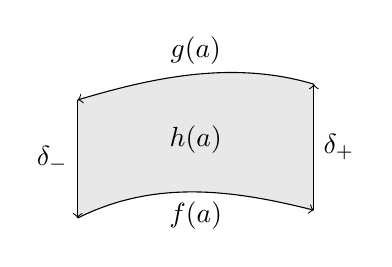
\begin{tikzpicture}[x=1cm,y=1cm,baseline=(current bounding box.center)]
\fill[gray!18] (0,0) .. controls (1,.5) and (2,.35) .. (3,.1) -- (3,1.7) .. controls (2,2) and (1,1.8) .. (0,1.5) -- cycle;
\draw[->] (0,0) .. controls (1,.5) and (2,.35) .. (3,.1) node[midway,below] {$f(a)$};
\draw[->] (3,.1) -- (3,1.7) node[midway,right] {$\delta_+$};
\draw[->] (3,1.7) .. controls (2,2) and (1,1.8) .. (0,1.5) node[midway,above] {$g(a)$};
\draw[->] (0,1.5) -- (0,0) node[midway,left] {$\delta_-$};
\node at (1.5,1) {$h(a)$};
\end{tikzpicture}
\end{center}
这意在表示 $f$ 与 $g$ 之间的一个同伦作用于 $X$ 中的一个链 $a$ 上的效果: $h(a)$ 是通过把 $a\times[0,1]$ 映到 $Y$ 而得到的链, 在限制到 $a\times\{0\}$ 时得到 $f(a)$, 在限制到 $a\times\{1\}$ 时得到 $g(a)$. 注意 $h(a)$ 是一个维数比 $a$ 的维数高 $1$ 的链, 并且这个链 $h(a)$ 的边界 $\partial h(a)$ 由 $f(a)$, $g(a)$ 以及 $h$ 在 $a$ 的边界 $\partial a$ 上的限制组成; 逆时针取边界,
\[
\partial h(a)=g(a)-\delta_+-f(a)+\delta_-=g(a)-f(a)-h(\partial a),
\]
(从图上看起来是这样! 这里给出的充其量只是一个可信性论证; 它可以严格化, 但那是别人的事).
于是
\[
g(a)-f(a)=\partial h(a)+h(\partial a).
\]
由于在同调中边界消逝, $f(a)$ 与 $g(a)$ 将在同调中一致.
下面就是把这一令人愉快的几何情形翻译成代数:

\begin{definition}\label{def:4.8-homotopy}
两个上链复形态射
\[
a^\bullet,\beta^\bullet:L^\bullet\to M^\bullet
\]
之间的一个\emph{同伦} (homotopy) $h$ 是一族态射
\[
h^i:L^i\to M^{i-1}
\]
使得对所有 $i$,
\[
\beta^i-a^i=d_M^{i-1}\circ h^i+h^{i+1}\circ d_L^i.
\]
我们说 $a^\bullet$ \emph{同伦于} (homotopic to) $\beta^\bullet$, 并记作 $a^\bullet\sim\beta^\bullet$, 如果存在 $a^\bullet$ 与 $\beta^\bullet$ 之间的一个同伦.
\end{definition}

\indent 我们这里处理的是上链复形; 这就解释了如下事实: 虽然在拓扑情形 (我们关心的是链而非上链) 中, 同伦会把维数往上移, 但在定义~\ref{def:4.8-homotopy} 中它却把次数往下移.
抛开其拓扑动机不谈, 同伦并不那么容易直观想象. 下面的图表\emph{并不}被假定为交换的:
\begin{center}
\begin{tikzcd}[column sep=small,row sep=large]
\cdots\ar[r]&L^i\ar[r,"d_L^i"]\ar[d,shift left=.7ex,"a^i"]\ar[d,shift right=.7ex,"\beta^i"']\ar[dl,"h^i"']&L^{i+1}\ar[r,"d_L^{i+1}"]\ar[d,shift left=.7ex,"a^{i+1}"]\ar[d,shift right=.7ex,"\beta^{i+1}"']\ar[dl,"h^{i+1}"']&\cdots\\
\cdots\ar[r]&M^i\ar[r,"d_M^i"']&M^{i+1}\ar[r]&\cdots
\end{tikzcd}
\end{center}
这些方块一般并不交换; 相反, 有
\[
d_M^{i-1}\circ h^i+h^{i+1}\circ d_L^i=\beta^i-\alpha^i.
\]
态射 $h^i$ 通常并不定义一个复形态射 $L^\bullet\to M[-1]^\bullet$: 这个图表中的菱形并不被要求交换.

\begin{definition}\label{def:4.9-homotopy-equivalence}
一个态射 $a^\bullet:L^\bullet\to M^\bullet$ 是一个\emph{同伦等价} (homotopy equivalence), 如果存在态射 $\beta^\bullet:M^\bullet\to L^\bullet$ 使得 $\beta^\bullet\circ a^\bullet\sim\mathrm{id}_{L^\bullet}$ 且 $a^\bullet\circ\beta^\bullet\sim\mathrm{id}_{M^\bullet}$. 如果存在如上那样一个同伦等价 $L^\bullet\to M^\bullet$, 就说复形 $L^\bullet$, $M^\bullet$\emph{同伦等价} (homotopy equivalent).
\end{definition}

\indent 读者应当验证 $\sim$ 是一个等价关系, 并且``复形的同伦等价''也是一个等价关系 (习题~\ref{ex:4.4}). 进一步, 这些关系显然与态射的简单运算相容 (习题~\ref{ex:4.5} 与习题~\ref{ex:4.6}).

\begin{proposition}\label{prop:4.10-homotopy-same-cohomology}
如果 $a^\bullet,\beta^\bullet:L^\bullet\to M^\bullet$ 是复形的同伦态射, 那么 $a^\bullet,\beta^\bullet$ 在同调上诱导相同的态射: $H^\bullet(L^\bullet)\to H^\bullet(M^\bullet)$.
\end{proposition}

\begin{proof}
设 $[\ell]\in H^i(L^\bullet)$. 则 $\ell$ 由满足 $d_L^i(\ell)=0$ 的元素 $\ell\in L^i$ 代表, 而它在 $H^i(M^\bullet)$ 中由 $a^\bullet$ (相应地, $\beta^\bullet$) 诱导的像由 $\alpha^i(\ell)$ (相应地, $\beta^i(\ell)$) $\in M^i$ 代表. 由于 $a^\bullet,\beta^\bullet$ 同伦, 依定义~\ref{def:4.8-homotopy} 存在态射 $h^i$ 使得
\[
\beta^i(\ell)-\alpha^i(\ell)=d_M^{i-1}(h^i(\ell))+h^{i+1}(d_L^i(\ell)).
\]
由于 $\ell\in\Ker d_L^i$, 末项消逝. 这说明
\[
\beta^i(\ell)-\alpha^i(\ell)\in\Image d_M^{i-1},
\]\erratumfootnote{此处官方勘误明确所取像的微分应带上复形下标，即写作 $\operatorname{im}d^{i-1}_{M^\bullet}$。}
从而 $\beta^i(\ell)-\alpha^i(\ell)$ 在 $H^i(M^\bullet)$ 中消逝, 这正是所需.
\end{proof}

\indent 例如, 如果 $a^\bullet$ 同伦于恒等态射, 那么由推论~\ref{cor:4.2-mapping-cone-exact} 知 $a^\bullet$ 的锥必然正合. 直接验证这个事实是一个很好的练习 (习题~\ref{ex:4.8}).

\begin{corollary}\label{cor:4.11-homotopy-equiv-cohomology}
同伦等价的复形有同构的上同调.
\end{corollary}

\begin{proof}
确实, 态射 $a^\bullet:L^\bullet\to M^\bullet$, $\beta^\bullet:M^\bullet\to L^\bullet$ 满足 $\beta^\bullet\circ a^\bullet$ 与 $a^\bullet\circ\beta^\bullet$ 都同伦于恒等态射, 那么由命题~\ref{prop:4.10-homotopy-same-cohomology} 它们在同调中诱导出互逆的态射.
\end{proof}

\begin{remark}\label{rmk:4.12-homotopy-equiv-qiso}
换句话说, 复形的同伦等价是拟同构. 这还没有解决``拟同构不可逆''这个``问题'', 因为例~\ref{ex:4.6-z2z-quasi-iso} 表明拟同构即便在同伦意义下也未必可逆. 换言之,``同伦等价''是比``拟同构''更严苛的概念. 我们在 \S\ref{subsec:5.3-proj-inj} 将要研究内射/投射模的复形的一个原因, 恰恰就在于: 对于 (有界的) 内射或投射模复形, 拟同构与同伦等价是等价的概念. 既然同伦等价是复形上的一个现成的等价关系, 这将绕过为把``拟同构''理解成一个等价关系所需的任何技术性细节.
\end{remark}

\indent 推论~\ref{cor:4.11-homotopy-equiv-cohomology} 是在一类有趣的例子中使 \S\ref{subsec:3.1-basic} 中提出的策略得以成立的那个主要技术性理由. 正如我们将适时看到的, 在这些例子中相关上链复形的上同调最终将不依赖于种种选取, 因为这些选取将产生同伦的复形.
另一个关键的观察是: 同伦等价被任何加性函子保持. 假设 $\mathcal A,\mathcal B$ 是 Abel 范畴, 并且
\[
F:\mathcal A\longrightarrow\mathcal B
\]
是一个加性函子 (定义~\ref{def:additive-category}). 那么它保持分次, 从而诱导一个加性函子
\[
\cate{C}(F):\cate{C}(\mathcal A)\longrightarrow\cate{C}(\mathcal B).
\]

\begin{lemma}\label{lem:4.13-additive-functor-homotopy}
沿用上面的 $F$. 如果在 $\cate{C}(\mathcal A)$ 中 $a^\bullet\sim\beta^\bullet$, 那么在 $\cate{C}(\mathcal B)$ 中 $\cate{C}(F)(a^\bullet)\sim\cate{C}(F)(\beta^\bullet)$; 并且如果 $L^\bullet$ 与 $M^\bullet$ 是 $\cate{C}(\mathcal A)$ 中同伦等价的复形, 那么 $\cate{C}(F)(L^\bullet)$ 与 $\cate{C}(F)(M^\bullet)$ 是 $\cate{C}(\mathcal B)$ 中同伦等价的复形.
\end{lemma}

\begin{proof}
第二个断言由第一个推出. 第一个是 $F$ 为加性这一事实的直接推论. 确实, 若 $h$ 是 $a^\bullet,\beta^\bullet:L^\bullet\to M^\bullet$ 之间的一个同伦, 则
\[
\beta^i-a^i=d_M^{i-1}\circ h^i+h^{i+1}\circ d_L^i.
\]
由于 $F$ 保持 Hom-集上的加性结构, 这推出
\[
F(\beta^i)-F(\alpha^i)=F(d_M^{i-1})\circ F(h^i)+F(h^{i+1})\circ F(d_L^i),
\]
表明态射族 $F(h^i)$ 给出了 $F(a^\bullet)$ 与 $F(\beta^\bullet)$ 之间的一个同伦.
\end{proof}

\indent 请注意, 对拟同构相应的陈述并不成立 (习题~\ref{ex:4.15}): 一个加性函子并不保持拟同构 (而正合函子则保持).
引理~\ref{lem:4.13-additive-functor-homotopy} 蕴涵: 在应用一个加性函子之后, 推论~\ref{cor:4.11-homotopy-equiv-cohomology} 的结论仍然成立:

\begin{theorem}\label{thm:4.14-additive-functor-cohomology}
设 $F:\mathcal A\to\mathcal B$ 是两个 Abel 范畴之间的一个加性函子. 如果 $L^\bullet,M^\bullet$ 是 $\cate{C}(\mathcal A)$ 中同伦等价的复形, 那么
\[
H^\bullet\bigl(\cate C(F)(L^\bullet)\bigr)\cong
H^\bullet\bigl(\cate C(F)(M^\bullet)\bigr).
\]
\end{theorem}

\indent 在我们已经做过的所有这些准备工作之后, 这个陈述的证明本质上是显而易见的, 因此留给读者 (习题~\ref{ex:4.16}).
我们赋予这个陈述以定理的地位, 是因为它正是我们所追求的策略的根源. 定理~\ref{thm:4.14-additive-functor-cohomology} 的内容是: 任何一个把某个数学对象联系到一个``在同伦意义下确定''的上链复形的机制, 都将会产生一大批有趣的不变量: 对你的任意一个这样的复形作用你最喜欢的加性函子, 取上同调, 而定理~\ref{thm:4.14-additive-functor-cohomology} 保证所得结果将不依赖于具体所选的复形. 这正是 §VIII.\ref{subsec:tor-functors} 与 §VIII.\ref{subsec:ext-functors} 中关于 Tor 与 Ext 函子定义之选取无关性的种种论断 (的一部分) 理由所在, 正如我们将在章末看到的那样 (\S\ref{sec:derived-functors}, 特别是例~\ref{ex:7.6-tor} 与例~\ref{ex:7.7-ext}).

\subsection*{习题}
\phantomsection
\addcontentsline{toc}{subsection}{习题}

\begin{prob}\label{ex:4.1}
验证一个复形态射的锥是一个复形. [\,\ref{subsec:4.1-mapping-cone}\,]
\end{prob}

\begin{prob}\label{ex:4.2}
设 $L^\bullet=\cdots\to 0\to L\to 0\to\cdots$ 与 $M^\bullet=\cdots\to 0\to M\to 0\to\cdots$ 是两个集中在 0 次的复形. 于是给出一个态射 $a^\bullet:L^\bullet\to M^\bullet$ 就等同于给出一个态射 $a:L\to M$. 描述这种情形下的映射锥及其上同调.
\end{prob}

\begin{prob}\label{ex:4.3}
设 $a^\bullet:L^\bullet\to M^\bullet$ 是一个有界复形态射. 注意映射锥 $\mathrm{MC}(a)^\bullet$ 也是有界的; 于是三个复形 $L^\bullet$, $M^\bullet$, $\mathrm{MC}(a)^\bullet$ 都有良定义的 Euler 示性数 (见习题~\ref{ex:3.15}). 证明
\[
\chi(\mathrm{MC}(a)^\bullet)=\chi(M^\bullet)-\chi(L^\bullet).
\]
\end{prob}

\begin{prob}\label{ex:4.4}
证明复形态射之间的同伦关系, 以及复形之间的同伦等价关系, 都是等价关系. [\,\ref{subsec:4.3-homotopy}, \S\ref{sec:9.6-resolutions}\,]
\end{prob}

\begin{prob}\label{ex:4.5}
设 $\alpha_k^\bullet,\beta_k^\bullet:L_k^\bullet\to M_k^\bullet$, $k=0,1$, 是上链复形之间的态射. 假设 $\alpha_0^\bullet\sim\beta_0^\bullet$, $\alpha_1^\bullet\sim\beta_1^\bullet$. 证明作为态射 $L_0^\bullet\oplus L_1^\bullet\to M_0^\bullet\oplus M_1^\bullet$ 有 $\alpha_0^\bullet\oplus\alpha_1^\bullet\sim\beta_0^\bullet\oplus\beta_1^\bullet$.\erratumfootnote{此处官方勘误为习题中的每个复形与态射补上圆点记号 $\bullet$，以明确它们是上链复形（及其间的态射）而非单个对象。} [\,\ref{subsec:4.3-homotopy}\,]
\end{prob}

\begin{prob}\label{ex:4.6}
设 $a^\bullet,a_0,a_1:L^\bullet\to M^\bullet$ 与 $\beta^\bullet,\beta_0,\beta_1:M^\bullet\to N^\bullet$ 是上链复形之间的态射.
\begin{itemize}
\item[(i)] 假设 $a^\bullet\sim 0$ 或 $\beta^\bullet\sim 0$. 证明 $\beta^\bullet\circ a^\bullet\sim 0$.
\item[(ii)] 假设 $a_0\sim a_1$ 且 $\beta_0\sim\beta_1$. 证明 $\beta_0\circ a_0\sim\beta_1\circ a_1$.
\end{itemize}
(提示: 用 (i), 同时把理想记在心里.) [\,\ref{subsec:4.3-homotopy}, \S\ref{subsec:5.2-homotopic-category}, \S\ref{subsec:5.4-homotopy-quasi}, \S\ref{subsec:5.5-proof}\,]
\end{prob}

\begin{prob}\label{ex:4.7}
证明: 同伦于一个给定态射的、复形 $L^\bullet\to M^\bullet$ 的态射组成的等价类, 由一族态射 $h^i:L^i\to M^{i-1}$ 的集合参数化, 模掉由复形态射 $L[1]^\bullet\to M^\bullet$ 组成的子集合.
\end{prob}

\begin{prob}\label{ex:4.8}
设 $a^\bullet$ 是一个复形态射, 且同伦于恒等态射. 不借助推论~\ref{cor:4.2-mapping-cone-exact} 直接证明 $a^\bullet$ 的映射锥是正合的. [\,\ref{subsec:4.3-homotopy}\,]
\end{prob}

\begin{prob}\label{ex:4.9}
设 $a^\bullet:L^\bullet\to M^\bullet$ 是一个上链复形态射. \emph{映射柱} $\mathrm{MCyl}(a)^\bullet$ 是次数 $i$ 处的对象为 $L^i\oplus L^{i+1}\oplus M^i$ 的上链复形, 其微分 $d_{\mathrm{MCyl}(a)}^i$ 定义为\index[sym1]{40@$\mathrm{MCyl}(a)^\bullet$}
\[
d_{\mathrm{MCyl}(a)}^i(\ell,\ell',m)=\bigl(d_L^i(\ell)+\ell',\,-d_L^{i+1}(\ell'),\, a^{i+1}(\ell')+d_M^i(m)\bigr).
\]
验证 $d_{\mathrm{MCyl}(a)}^{i+1}\circ d_{\mathrm{MCyl}(a)}^i=0$, 从而 $\mathrm{MCyl}(a)^\bullet$ 确实是一个上链复形. [\,\ref{ex:4.10}, \ref{ex:4.11}, \ref{ex:4.12}, \ref{ex:4.13}\,]
\end{prob}

\begin{prob}\label{ex:4.10}
从拓扑上说, 一个连续映射 $f:X\to Y$ 的映射柱是通过考虑 $X\times[0,1]$ 并用 $f$ 把 $X\times1$ 粘合到 $Y$ 上而得到的; 研究这个对象的 (上) 链就导出了习题~\ref{ex:4.9} 的代数映射柱.
正如我们在拓扑中得知的, 两个连续映射 $X\to Y$ 是同伦的, 当且仅当它们可以实现为从柱 $X\times[0,1]$ 到 $Y$ 的某个连续映射在 $X\times0$, $X\times1$ 上的限制. 注意这个柱就是 $\mathrm{id}_X$ 的映射柱.
证明两个上链映射 $a^\bullet,\beta^\bullet:L^\bullet\to M^\bullet$ 在定义~\ref{def:4.8-homotopy} 的意义下同伦, 当且仅当它们延拓为一个上链态射 $(-a^\bullet,h^\bullet,\beta^\bullet):\mathrm{MCyl}(\mathrm{id}_{L^\bullet})^\bullet\to M^\bullet$.
\end{prob}

\begin{prob}\label{ex:4.11}
在拓扑中, 映射锥可以通过在映射柱中把 $X\times0$ 捏成一点而得到 (cf. 习题~\ref{ex:4.9} 与 \S\ref{subsec:4.1-mapping-cone} 中对映射锥的描述).
在代数版本中, 这个收缩相当于对 $\mathrm{MCyl}(a)^\bullet$ 的第一个分量取商. 对上链态射 $a^\bullet:L^\bullet\to M^\bullet$, 证明存在一个上链复形的正合列
\[
0\longrightarrow L^\bullet\longrightarrow\mathrm{MCyl}(a)^\bullet\longrightarrow\mathrm{MC}(a)^\bullet\longrightarrow 0.
\]
[\,\ref{ex:4.14}\,]
\end{prob}

\begin{prob}\label{ex:4.12}
沿用习题~\ref{ex:4.9} 的记号 (特别地, 对一个上链态射 $a^\bullet:L^\bullet\to M^\bullet$), 证明存在一个上链复形的正合列
\[
0\longrightarrow M^\bullet\longrightarrow\mathrm{MCyl}(a)^\bullet\longrightarrow\mathrm{MC}(\mathrm{id}_{L^\bullet})^\bullet\longrightarrow 0.
\]
推得存在一个拟同构 $M^\bullet\to\mathrm{MCyl}(a)^\bullet$. [\,\ref{ex:4.13}, \ref{ex:4.14}\,]
\end{prob}

\begin{prob}\label{ex:4.13}
仍沿用习题~\ref{ex:4.9} 的记号, 定义映射 $p^\bullet:M^\bullet\to\mathrm{MCyl}(a)^\bullet$ 与 $q^\bullet:\mathrm{MCyl}(a)^\bullet\to M^\bullet$ 为
\[
p^i(m)=(0,0,m),\qquad q^i(\ell,\ell',m)=m-a^i(\ell).
\]
证明 $p^\bullet$, $q^\bullet$ 都是上链态射. 注意 $q^\bullet\circ p^\bullet=\mathrm{id}_{M^\bullet}$, 并证明 $p^\bullet\circ q^\bullet$ 同伦于 $\mathrm{id}_{\mathrm{MCyl}(a)^\bullet}$. (提示: $(\ell,\ell',m)\mapsto(0,\ell,0)$.)
\indent 由此推出 $M^\bullet$ 与 $\mathrm{MCyl}(a)^\bullet$ 同伦等价. 这强化了习题~\ref{ex:4.12} 的结论. [\,\ref{ex:4.14}\,]
\end{prob}

\begin{prob}\label{ex:4.14}
综合习题~\ref{ex:4.11}, \ref{ex:4.12}, \ref{ex:4.13}, 得出结论: 在同伦等价意义下, 一个上链态射 $a^\bullet:L^\bullet\to M^\bullet$ 可以被替换为一个单态射 $L^\bullet\hookrightarrow\mathrm{MCyl}(a)^\bullet$, 它在同调中诱导相同的态射 $H^\bullet(a^\bullet)$ (依同构 $H^\bullet(M^\bullet)\cong H^\bullet(\mathrm{MCyl}(a)^\bullet)$ 辨识), 并且它的余核就是映射锥 $\mathrm{MC}(a)^\bullet$.
\end{prob}

\begin{prob}\label{ex:4.15}
证明, 一般情形下, 加性函子并不保持拟同构. (提示: 例~\ref{ex:4.6-z2z-quasi-iso}.) 证明正合函子保持拟同构. (提示: 用映射锥.) [\,\ref{subsec:4.3-homotopy}, \S\ref{sec:9.6-resolutions}\,]
\end{prob}

\begin{prob}\label{ex:4.16}
证明定理~\ref{thm:4.14-additive-functor-cohomology}. [\,\ref{subsec:4.3-homotopy}\,]
\end{prob}

\section{同伦范畴·投射与内射复形}
\label{sec:homotopic-category}

我们在 §4 中试图传达的一个信息是: 虽然拟同构 (按定义!) 是保持上同调的上链复形态射, 因而可被视为``抓住了复形的上同调'', 但从应用的观点看, 同伦等价这一更强的概念实际上更为自然. 这正是定理~\ref{thm:4.14-additive-functor-cohomology} 的寓意: 同伦等价的复形具有相同的上同调, 其理由比仅仅由拟同构相连的复形要深刻得多. 如果我们总的目标是理解``使所有拟同构都可逆'' (亦即理解导出范畴 $D(\mathcal{A})$) 意味着什么, 那么我们不妨从使同伦等价可逆开始. 这就产生了一个新的范畴, 即复形的``同伦范畴'' $K(\mathcal{A})$, 我们在本节中加以探讨. 我们还将考察由投射与内射对象构成的有界复形在同伦方面的特殊地位: 对于这些复形, 拟同构必然是同伦等价. 验证这一点需要相当技术性的考量, 但它是为了理解 \S\ref{sec:9.6-resolutions} 中的导出范畴所必须的.

\subsection{同伦映射在导出范畴中被等同}
\label{subsec:5.1-derived-identify}

要看出这个``同伦范畴''是从 $C(\mathcal{A})$ 通往 $D(\mathcal{A})$ 途中的必经一站, 不妨回到我们在 \S\ref{subsec:4.2-quasi-iso-derived} 末尾所做的较为高明的考虑. 再次考虑任一加性函子
\[
\mathcal{F}:C(\mathcal{A})\longrightarrow\mathcal{D}
\]
它把拟同构变为同构. 最简单的这种函子是上同调; 而万有的是由 $C(\mathcal{A})$ 到那个神秘的导出范畴 $D(\mathcal{A})$ 的函子. 我们在命题~\ref{prop:4.10-homotopy-same-cohomology} 中已经验证过: 同伦的映射在上同调中诱导出同一个态射. 对如上任一函子 $\mathcal{F}$, 情形难道不是如此吗? 确实如此!

\begin{lemma}\label{lem:5.1-homotopic-identified}
设 $\mathcal{F}:C(\mathcal{A})\to\mathcal{D}$ 是一个加性函子, 使得对 $C(\mathcal{A})$ 中所有的拟同构 $p^\bullet$ 都有 $\mathcal{F}(p^\bullet)$ 在 $\mathcal{D}$ 中是同构.

设 $\alpha^\bullet,\beta^\bullet:L^\bullet\to M^\bullet$ 是 $C(\mathcal{A})$ 中同伦的态射. 则在 $\mathcal{D}$ 中有 $\mathcal{F}(\alpha^\bullet)=\mathcal{F}(\beta^\bullet)$.
\end{lemma}

\begin{proof}
等价地 (由于 $\mathcal{F}$ 是加性的), 我们验证: 若 $\alpha^\bullet\sim 0$, 则 $\mathcal{F}(\alpha^\bullet)=0$. 由引理~\ref{lem:4.7-quasi-iso-functor-zero}, 只需证明 $\alpha^\bullet$ 经过一个正合复形分解.

这个正合复形就是恒等映射 $\mathrm{id}_{L^\bullet}:L^\bullet\to L^\bullet$ 的映射锥 $MC(\mathrm{id}_{L^\bullet})^\bullet$. 回忆 (\S\ref{subsec:4.1-mapping-cone}) 有
\[
MC(\mathrm{id}_{L^\bullet})^i=L^{i+1}\oplus L^i,
\]
其微分定义为
\[
d_{MC(\mathrm{id}_{L^\bullet})}(a,b)=\bigl(-d_L(a),\,a+d_L(b)\bigr).
\]
由于恒等映射平凡地是一个拟同构, $MC(\mathrm{id}_{L^\bullet})^\bullet$ 是一个正合复形 (推论~\ref{cor:4.2-mapping-cone-exact}). 映射
\[
L^i\longrightarrow MC(\mathrm{id}_{L^\bullet})^i,\qquad b\longmapsto (0,b)
\]
总与微分交换, 因而定义了一个复形态射 $L^\bullet\to MC(\mathrm{id}_{L^\bullet})^\bullet$. 相反地, 一个映射 $MC(\mathrm{id}_{L^\bullet})^\bullet\to M^\bullet$ 一般并不存在. 但在我们的假设下有一个同伦 $\alpha^\bullet\sim 0$, 即一族态射 $h^i:L^i\to M^{i-1}$ 使得
\[
\alpha^i=d_M\circ h^i+h^{i+1}\circ d_L.
\]
定义一族态射 $\gamma^i:MC(\mathrm{id}_{L^\bullet})^i\to M^i$ 为
\[
\gamma^i(a,b)=h^{i+1}(a)+\alpha^i(b).
\]
显然复合
\[
L^i\longrightarrow MC(\mathrm{id}_{L^\bullet})^i\longrightarrow M^{i}
\]
就是 $\alpha^{i}$. 现在只需验证这族 $\gamma^{i}$ 定义了一个复形态射; 这将表明 $\alpha^\bullet$ 经过正合复形 $MC(\mathrm{id}_{L^\bullet})^\bullet$ 分解, 从而 $\mathcal{F}(\alpha^\bullet)=0$ (由引理~\ref{lem:4.7-quasi-iso-functor-zero}), 完成本引理的证明. 也就是说, 我们必须对所有 $i$ 验证如下图表交换:
\begin{center}
\begin{tikzcd}
MC(\mathrm{id}_{L^\bullet})^{i-1} \ar[r, "d_{MC(\mathrm{id}_{L^\bullet})}^{i-1}"] \ar[d, "\gamma^{i-1}"'] & MC(\mathrm{id}_{L^\bullet})^i \ar[d, "\gamma^{i}"] \\
M^{i-1} \ar[r, "d_M^{i-1}"'] & M^{i}
\end{tikzcd}
\qquad(*)
\end{center}
(*) 的左边作用如下:
\[
(a,b)\longmapsto h^{i}(a)+\alpha^{i-1}(b)\longmapsto d_M\bigl(h^{i}(a)+\alpha^{i-1}(b)\bigr).
\]
右边作用为
\[
(a,b)\longmapsto \bigl(-d_L(a),\,a+d_L(b)\bigr)\longmapsto -h^{i+1}\bigl(d_L(a)\bigr)+\alpha^{i}\bigl(a+d_L(b)\bigr).
\]
于是所需的等式为
\[
d_M\bigl(h^{i}(a)\bigr)+d_M\bigl(\alpha^{i-1}(b)\bigr)=-h^{i+1}\bigl(d_L(a)\bigr)+\alpha^{i}(a)+\alpha^{i}\bigl(d_L(b)\bigr),
\]
或者等价地,
\[
\bigl(d_M\circ h^{i}+h^{i+1}\circ d_L-\alpha^{i}\bigr)(a)=\bigl(\alpha^{i}\circ d_L-d_M\circ\alpha^{i-1}\bigr)(b),
\]
其中 $a\in L^{i}$, $b\in L^{i-1}$. 但两边都为 $0$: 右边是因为 $\alpha^\bullet$ 是一个复形态射, 左边是因为 $h^{i}$ 是一个同伦 $\alpha^\bullet\sim 0$.
\end{proof}

引理~\ref{lem:5.1-homotopic-identified} 告诉我们: 每一个把拟同构变为同构的函子, 都必须经过由 $C(\mathcal{A})$ 把同伦的态射等同起来而得到的范畴分解. 现在该定义这个范畴了.

\index{fuxingdetonglunfanchou@复形的同伦范畴(homotopy category of complexes)}\subsection{复形的同伦范畴的定义}
\label{subsec:5.2-homotopic-category}

\begin{definition}\label{def:5.2-homotopic-category}
设 $\mathcal{A}$ 是一个 Abel 范畴. $\mathcal{A}$ 中上链复形的\emph{同伦范畴} $K(\mathcal{A})$ 是指这样一个范畴: 其对象就是 $\mathcal{A}$ 中的上链复形 (亦即与 $C(\mathcal{A})$ 相同的对象), 而其态射为
\[
\Hom_{K(\mathcal{A})}(L^\bullet,M^\bullet):=\Hom_{C(\mathcal{A})}(L^\bullet,M^\bullet)/\!\sim,
\]
其中 $\sim$ 是同伦关系.
\end{definition}

\indent 是的, 但它真的是一个范畴吗? 回忆同伦关系 $\sim$ 尊重复合 (习题~\ref{ex:4.6}); 换言之, 复合运算
\[
\Hom_{C(\mathcal{A})}(L^\bullet,M^\bullet)\times\Hom_{C(\mathcal{A})}(M^\bullet,N^\bullet)\longrightarrow\Hom_{C(\mathcal{A})}(L^\bullet,N^\bullet)
\]
确实下降到运算
\[
\Hom_{K(\mathcal{A})}(L^\bullet,M^\bullet)\times\Hom_{K(\mathcal{A})}(M^\bullet,N^\bullet)\longrightarrow\Hom_{K(\mathcal{A})}(L^\bullet,N^\bullet).
\]
核查范畴公理是例行公事, 留给耐心的读者.

有界变体 $K^-(\mathcal{A})$, $K^+(\mathcal{A})$ 等, 可以类似地由 $C^-(\mathcal{A})$, $C^+(\mathcal{A})$ 等得到. 下面的考虑对这一切版本都适用. 进一步的变体 $K^-(P)$ 与 $K^+(I)$ (其中要求复形分别由 $\mathcal{A}$ 的投射对象与内射对象组成; 参见 §\ref{subsec:5.3-proj-inj}) 也将起到至关重要的作用.\index[sym1]{30@$K^+(I)$}\index[sym1]{31@$K^-(P)$}
至于同伦范畴所蕴含的一般结构, 我们有

\begin{lemma}\label{lem:5.3-K-additive}
设 $\mathcal{A}$ 是一个 Abel 范畴. 则复形的同伦范畴 $K(\mathcal{A})$ 是一个加性范畴.
\end{lemma}

\begin{proof}
练习~\ref{ex:5.1}.
\end{proof}

\indent 然而请注意, 一般而言同伦范畴并不是 Abel 的. 事实的确如此: 同伦的映射一般并不具有相同的核或余核, 因而定义这些概念就成了问题. 正如我们在 \S\ref{subsec:3.4-triangles} 中已经提到, $K(\mathcal{A})$ 是一个三角范畴; ``典范三角'' 正是 \S\ref{subsec:4.1-mapping-cone} 中由态射的映射锥给出的那些三角. (我们将在 \S\ref{subsec:9.2-triangulated} 中简要描述这一情形.)

\indent 引入同伦范畴的主要动机在于: 同伦等价在 $K(\mathcal{A})$ 中成为同构. 更精确地说, 按定义存在一个函子
\[
C(\mathcal{A})\longrightarrow K(\mathcal{A}),
\]
它把每个对象映到``它自己'', 并把每个态射映到它的同伦类. $C(\mathcal{A})$ 中的同伦等价在 $K(\mathcal{A})$ 中成为同构, 因为关系 $\alpha^\bullet\circ\beta^\bullet\sim\mathrm{id}$ 在 $C(\mathcal{A})$ 中变成了 $\alpha^\bullet\circ\beta^\bullet=\mathrm{id}$ 在 $K(\mathcal{A})$ 中. 同伦范畴正是由 $C(\mathcal{A})$ 通过把所有的同伦等价都彻底变成可逆而得到的.

\indent 于是我们可以把引理~\ref{lem:5.1-homotopic-identified} 重新解释为如下的``分解''结果:

\begin{proposition}\label{prop:5.4-factor-through-K}
设 $\mathcal{F}:C(\mathcal{A})\to\mathcal{D}$ 是一个加性函子, 使得对 $C(\mathcal{A})$ 中所有的拟同构 $p^\bullet$ 都有 $\mathcal{F}(p^\bullet)$ 在 $\mathcal{D}$ 中是同构. 则 $\mathcal{F}$ 唯一地经过 $K(\mathcal{A})$ 分解:
\begin{center}
\begin{tikzcd}
C(\mathcal{A}) \ar[rr, "\mathcal{F}"] \ar[dr, "\pi"'] & & \mathcal{D} \\
& K(\mathcal{A}) \ar[ur, dashed, "\exists!\,\overline{\mathcal{F}}"']
\end{tikzcd}
\end{center}
\end{proposition}

\begin{proof}
练习~\ref{ex:5.2}.
\end{proof}

\indent 特别地, 必定存在一个从 $K(\mathcal{A})$ 到那个更微妙的导出范畴 $D(\mathcal{A})$ 的唯一函子. 当然, 对所有这些对象的有界版本, 情形是类似的: 从适当有界复形到相应导出范畴的自然函子, 都唯一地经过相应的同伦范畴分解:
\begin{center}
\begin{tikzcd}[row sep=large]
C^-(\mathcal{A}) \ar[r] & K^-(\mathcal{A}) \ar[r] & D^-(\mathcal{A}) \\
C^+(\mathcal{A}) \ar[r] & K^+(\mathcal{A}) \ar[r] & D^+(\mathcal{A})
\end{tikzcd}
\end{center}

\indent 命题~\ref{prop:5.4-factor-through-K} 的一个特例是如下事实: $C(\mathcal{A})$ (相应地, $C^-(\mathcal{A})$, $C^+(\mathcal{A})$) 上的上同调函子下降到 $K(\mathcal{A})$ (相应地, $K^-(\mathcal{A})$, $K^+(\mathcal{A})$) 上的一个函子. 这一事实也可由命题~\ref{prop:4.10-homotopy-same-cohomology} 直接推出: 同伦的映射在上同调中诱导出同一个态射.

\subsection{投射与内射对象构成的复形}
\label{subsec:5.3-proj-inj}

我们应当追问: $K(\mathcal{A})$ 距离 $D(\mathcal{A})$ 可能有多远. 我们在 $K(\mathcal{A})$ 中已经把所有同伦等价都倒转了, 但并非所有拟同构都是同伦等价: 请牢记例~\ref{ex:4.6-z2z-quasi-iso}. 如果我们想把 $K(\mathcal{A})$ 视作 $D(\mathcal{A})$ 的第一个近似, 就应当聚焦于这样一类复形: 在其中拟同构与同伦等价之间本质上没有区别.

\indent 事实表明确有这样的复形: 那些由投射或内射对象构成的复形.

\indent 回忆 (定义~VIII.\ref{def:projective-injective}) 一个 $R$-模 $M$ 是``投射的'', 如果函子 $\Hom_R(M,-)$ 是正合的; 它是``内射的'', 如果 $\Hom_R(-,M)$ 是正合的. 我们可以在任何 Abel 范畴中采用这些定义:

\begin{definition}\label{def:5.5-projective-injective}
设 $\mathcal{A}$ 是一个 Abel 范畴. $\mathcal{A}$ 的一个对象 $P$ 是\emph{投射的}, 如果函子 $\Hom_{\mathcal{A}}(P,-)$ 是正合的. 一个对象 $Q$ 是\emph{内射的}, 如果函子 $\Hom_{\mathcal{A}}(-,Q)$ 是正合的.
\end{definition}

\indent 诸如引理~VIII.\ref{lem:projective-injective-lifting} 那样的普遍评注, 或 §VIII.\ref{subsec:projectives-injectives} 末尾关于序列分裂的那些评论, 在任何 Abel 范畴中都成立; 对读者而言, 一个很好的练习就是收集所有这类信息, 并验证它们在新的语境中确实成立.

\indent 还要注意到, 在这一普遍程度下, 该理论中处理内射对象的部分, 是处理投射对象的部分的一面忠实的镜子. 这当然并非巧合: 一个 Abel 范畴的对立范畴仍是 Abel 的 (习题~\ref{ex:1.10}), 而一方的投射对象在另一方就成了内射对象. 因此, 确实只需对任意 Abel 范畴中的投射对象证明陈述即可: 关于内射对象的相应陈述将自动随之成立.

\indent 这种对偶的状况不应被推得太远: 在一个固定的 Abel 范畴中, 投射与内射对象可能呈现出非常不同的特征. 例如, §VIII.\ref{subsec:projective-modules} 与 §VIII.\ref{subsec:injective-modules} 中给出的刻画用到了范畴 $R\dcate{-Mod}$ 的具体性质, 因而不应指望它们在任意 Abel 范畴中有简单的对应物.

\indent 我们将用 $\mathcal{P}$ (相应地, $\mathcal{I}$) 记由投射 (相应地, 内射) 对象决定的 $\mathcal{A}$ 的全子范畴. 当然, 在任何有趣的情形下这些都不是 Abel 范畴. 注意一个 Abel 范畴很可能没有任何非平凡的投射或内射对象.

\begin{example}\label{ex:5.6-finabelian}
有限 Abel 群的范畴是 Abel 的 (真令人吃惊), 但它不包含任何非平凡的投射或内射对象 (练习~\ref{ex:5.5}).
\end{example}

\begin{definition}\label{def:5.7-enough}
一个 Abel 范畴 $\mathcal{A}$ \emph{有充足投射对象}, 如果对每个对象 $A\in\mathcal{A}$, 都存在一个投射对象 $P\in\mathcal{A}$ 以及一个满态射 $P\twoheadrightarrow A$. 该范畴\emph{有充足内射对象}, 如果对每个对象 $A\in\mathcal{A}$, 都存在一个内射对象 $Q\in\mathcal{A}$ 以及一个单态射 $A\hookrightarrow Q$.
\end{definition}

\indent 这些定义对读者而言并不新鲜, 因为我们在 §VIII.\ref{sec:projective-injective-ext} 中碰到过它们: 特别是我们已经观察到, 对每个交换环 $R$, $R\dcate{-Mod}$ 都有充足投射对象 (这一点毫不困难: 自由模及其直和项是投射的, 见命题~VIII.\ref{prop:projective-summand-free}) 与充足内射对象 (这一点困难得多; 我们在推论~VIII.\ref{cor:enough-injectives} 中证明了它).

\index{Abel qun@Abel 群(abelian group)!fanchou@范畴(category)}\indent 例~\ref{ex:5.6-finabelian} 表明, 我们不应指望一个 Abel 范畴 $\mathcal{A}$ 具有上述两种性质中的任何一种. 能够说明存在充足内射对象的一个重要情形, 是拓扑空间上 Abel 群层构成的范畴; 这是把层上同调定义为一个``导出函子''的关键一步. 一般而言, 层范畴没有充足投射对象. 另一方面, 有限生成 Abel 群范畴有充足投射对象, 却没有充足 (事实上没有任何非平凡) 内射对象. 事情就是这样.

\subsection{K(A) 中的同伦等价与拟同构}
\label{subsec:5.4-homotopy-quasi}

正如我们已经提到的, 我们将感兴趣于 $K(\mathcal{A})$ 中由 $\mathcal{A}$ 的投射或内射对象复形所决定的某些子范畴.

\begin{definition}\label{def:5.8-KP-KI}
我们用 $K^-(P)$ 记 $K(\mathcal{A})$ 的由 $\mathcal{A}$ 的投射对象的有界上方复形构成的全子范畴, 并用 $K^+(I)$ 记 $K(\mathcal{A})$ 的由 $\mathcal{A}$ 的内射对象的有界下方复形构成的全子范畴.
\end{definition}

\indent 本节余下部分的主要结果是如下定理:

\begin{theorem}\label{thm:5.9-quasi-is-homotopy-equiv}
设 $\mathcal{A}$ 是一个 Abel 范畴, 并设 $\alpha^\bullet:P^\bullet\to \widetilde{P}^\bullet$ (相应地, $\alpha^\bullet:Q^\bullet\to\widetilde{Q}^\bullet$) 是 $\mathcal{A}$ 中两个投射对象的有界上方复形 (相应地, 内射对象的有界下方复形) 之间的一个拟同构. 则 $\alpha^\bullet$ 是一个同伦等价.
\end{theorem}

\begin{corollary}\label{cor:5.10-quasi-iso-invertible}
在 $K^-(P)$ 与 $K^+(I)$ 中, 拟同构的 (同伦类) 都是同构.
\end{corollary}

\indent 也就是说, 投射或内射对象的有界复形之间所有的拟同构, 在 $K^-(P)$, $K^+(I)$ 中``已经''被倒转了. 因此, 这些范畴非常接近于相应的导出范畴. 事实上, 我们将会看到: 如果 $\mathcal{A}$ 有充足投射对象, 那么 $K^-(P)$ 就``足以''描述 $D^-(\mathcal{A})$ (其精确含义将变得更明确); 类似地, 如果 $\mathcal{A}$ 有充足内射对象, 则 $K^+(I)$ 充当了 $D^+(\mathcal{A})$ 的一个具体实现.

\indent 定理~\ref{thm:5.9-quasi-is-homotopy-equiv} 的证明需要若干准备, 它们进一步澄清了投射与内射对象复形在同伦方面扮演的角色.

\indent 说 $C(\mathcal{A})$ 中的一个复形 $N^\bullet$ 正合, 有一种绕弯的说法是: 恒等映射 $\mathrm{id}_{N^\bullet}$ 与平凡映射 $0$ 在上同调中诱导出同一个态射——正如它们在彼此同伦时本该有的那样. 然而, 要构造这样一个恒等映射不同伦于 $0$ 的正合复形的例子却很容易. 正如读者将验证的 (练习~\ref{ex:5.11}), 这与该复形是否分裂有关; 一般地, 如果一个复形 $N^\bullet$ 满足 $\mathrm{id}_{N^\bullet}$ 同伦于 $0$, 则称它是``分裂正合''的. 牢记投射或内射对象会``迫使''序列分裂, 那么如下事实或许就不那么令人惊讶了: 对于由投射或内射对象构成的有界正合复形, 恒等映射确实同伦于 $0$.

\indent 为了验证这一点, 我们研究能保证态射同伦于 $0$ 的特殊条件.

\begin{lemma}\label{lem:5.11-proj-nullhomotopy}
设 $p^\bullet$ 是 Abel 范畴 $\mathcal{A}$ 中一个由投射对象构成的复形, 满足对 $i>0$ 有 $p^{i}=0$; 并设 $L^\bullet$ 是 $C(\mathcal{A})$ 中一个复形, 满足对 $i<0$ 有 $H^{i}(L^\bullet)=0$.

设 $\alpha^\bullet:p^\bullet\to L^\bullet$ 是一个在上同调上诱导出零态射的态射. 则 $\alpha^\bullet$ 同伦于 $0$.
\end{lemma}

\indent 读者将给出这一陈述的``内射''版本: 它处理从一个在正次数处正合的复形, 到一个由内射对象构成的复形 $Q^\bullet$ (满足对 $i<0$ 有 $Q^{i}=0$) 的态射.

\begin{proof}
我们必须构造一族态射 $h^i:p^i\to L^{i-1}$, 如下图所示:
\[
\begin{tikzcd}[column sep=small,row sep=large]
\cdots\ar[r]&P^{-2}\ar[r,"d_P^{-2}"]\ar[d,"\alpha^{-2}"']\ar[dl,"h^{-2}"']&P^{-1}\ar[r,"d_P^{-1}"]\ar[d,"\alpha^{-1}"']\ar[dl,"h^{-1}"']&P^0\ar[r]\ar[d,"\alpha^0"']\ar[dl,"h^0"']&0\ar[r]\ar[d]\ar[dl,"h^1=0"']&\cdots\\
\cdots\ar[r]&L^{-2}\ar[r,"d_L^{-2}"']&L^{-1}\ar[r,"d_L^{-1}"']&L^0\ar[r]&L^1\ar[r]&\cdots
\end{tikzcd}
\]
也就是使得
\begin{equation*}
\alpha^i=d_L^{i-1}\circ h^i+h^{i+1}\circ d_P^i.
\tag{*}
\end{equation*}
当然, 对于 $i>0$ 必有 $h^{i}=0$. 对 $i=0$, 利用 $\alpha^\bullet$ 在上同调上诱导的映射为 $0$ 这一事实; 这说明 $\alpha^{0}$ 经过 $d_L$ 的象分解:
\begin{center}
\begin{tikzcd}
& P^0 \ar[d,"\alpha^0"] \ar[dl,dashed,"h^0"'] & \\
L^{-1} \ar[r,two heads] & \Image d_L^{-1} \ar[r,hook] & L^0
\end{tikzcd}
\end{center}
由于 $p^{0}$ 是投射的, 故存在态射 $h^{0}:p^{0}\to L^{-1}$ 使得 $\alpha^{0}=d_L^{-1}\circ h^{0}$, 正如所需.

\indent 对 $i\le 0$ 定义 $h^{i-1}$, 我们归纳地进行: 假设已经构造出满足 (*) 的 $h^{i}$ 与 $h^{i+1}$. 注意由 (*) (以及 $p^\bullet$ 是一个复形) 有下图所表示的归纳关系:
\[
\begin{tikzcd}[column sep=small,row sep=large]
\cdots\ar[r]&P^{i-1}\ar[r,"d_P^{i-1}"]\ar[d,"\alpha^{i-1}"']\ar[dl,dashed,"h^{i-1}"']&P^i\ar[r,"d_P^i"]\ar[d,"\alpha^i"']\ar[dl,"h^i"']&P^{i+1}\ar[d,"\alpha^{i+1}"']\ar[dl,"h^{i+1}"']\\
\cdots\ar[r]&L^{i-1}\ar[r,"d_L^{i-1}"']&L^i\ar[r,"d_L^i"']&L^{i+1}
\end{tikzcd}
\]
具体地说,
\[
d_L^{i-1}\bigl(\alpha^{i-1}-h^{i}\circ d_p^{i-1}\bigr)
=d_L(\alpha^{i-1})-d_L(h^{i}\circ d_p^{i-1})
=\alpha^{i}\circ d_p^{i-1}-\bigl(\alpha^{i}-h^{i+1}\circ d_p^{i}\bigr)\circ d_p^{i-1}=0,
\]
因为 $\alpha^\bullet$ 是上链复形态射且 $d_p^2=0$. 这表明 $\alpha^{i-1}-h^{i}\circ d_p^{i-1}$ 经过 $\Ker d_L^{i-1}$ 分解. 由于对 $i-1<0$ 有 $L^\bullet$ 在 $L^{i-1}$ 处正合, 故 $\Ker d_L^{i-1}=\Image d_L^{i-2}$. 因此我们又有一个分解
\begin{center}
\begin{tikzcd}
& P^{i-1} \ar[d,"\alpha^{i-1}-h^i d_P^{i-1}"] \ar[dl,dashed,"h^{i-1}"'] & \\
L^{i-2} \ar[r,two heads] & \Image d_L^{i-2} \ar[r,hook] & L^{i-1}
\end{tikzcd}
\end{center}
现在 $p^{i-1}$ 是投射的; 因此存在 $h^{i-1}:p^{i-1}\to L^{i-2}$ 使得
\[
\alpha^{i-1}-h^{i}\circ d_p^{i-1}=d_L^{i-2}\circ h^{i-1},
\]
这恰好就是归纳步骤所需.
\end{proof}

\begin{corollary}\label{cor:5.12-mor-to-exact-nullhomotopic}
设 $p^\bullet$ 是 Abel 范畴 $\mathcal{A}$ 中一个由投射对象构成的有界上方上链复形, 并设 $L^\bullet$ 是 $C(\mathcal{A})$ 中的一个正合复形.

则每个复形态射 $p^\bullet\to L^\bullet$ 都同伦于 $0$.
\end{corollary}

\indent 这由引理~\ref{lem:5.11-proj-nullhomotopy} (经过一个无妨的平移) 立即得出, 因为到正合复形的每个态射都别无选择, 只能在上同调中诱导出零态射.

\indent 推论~\ref{cor:5.12-mor-to-exact-nullhomotopic} 的``内射''版本是: 从一个正合复形 $L^\bullet$ 到一个由内射对象构成的有界下方复形 $Q^\bullet$ 的态射, 必然同伦于 $0$.

\indent 注意在所有这些考虑中, 复形 $p^\bullet$, $Q^\bullet$ 都被要求落在``有界''版本 $C^-(P)$, $C^+(I)$ 中: 所有对象应当在充分高或充分低的次数处消失. 这为引理~\ref{lem:5.11-proj-nullhomotopy} 证明中同伦的归纳构造提供了``起点''. 这是该理论中一个本质上无法回避的特征.

\begin{corollary}\label{cor:5.13-bounded-exact-nullhomotopic}
设 $p^\bullet$ (相应地, $Q^\bullet$) 是一个由投射对象构成的有界上方正合复形 (相应地, 由内射对象构成的有界下方正合复形). 则 $p^\bullet$ (相应地, $Q^\bullet$) 同伦等价于零复形.
\end{corollary}

\begin{proof}
练习~\ref{ex:5.12}.
\end{proof}

\indent 推论~\ref{cor:5.13-bounded-exact-nullhomotopic} 是定理~\ref{thm:5.9-quasi-is-homotopy-equiv} 所更充分捕捉的那个原理的首次显现: 我们刚刚验证了, 对于适当有界的投射或内射对象复形, ``拟同构于 $0$'' 与``同伦等价于 $0$''是一回事.

\indent 引理~\ref{lem:5.11-proj-nullhomotopy} 的另一个推论是如下评注, 它表明: 就来自投射对象复形的态射而言, 拟同构在同伦意义下是``非零因子''. 这在下一节中将很有用, 例如用来说明某些提升在同伦意义下是唯一确定的.

\begin{lemma}\label{lem:5.14-nonzero-divisor}
设 $\mathcal{A}$ 是一个 Abel 范畴, 并设 $\varphi^\bullet:L^\bullet\to M^\bullet$ 是 $C(\mathcal{A})$ 中的一个拟同构. 设 $p^\bullet$ 是一个由投射对象构成的有界上方复形, 并设 $\alpha^\bullet:p^\bullet\to L^\bullet$ 是一个上链复形态射, 使得复合 $\varphi^\bullet\circ\alpha^\bullet$ 同伦于零态射. 则 $\alpha^\bullet\sim 0$.
\end{lemma}

\begin{proof}
设 $h^{i}:p^{i}\to M^{i-1}$ 定义了 $\varphi^\bullet\circ\alpha^\bullet$ 与 $0$ 之间的一个同伦, 即
\[
-\varphi^i\circ\alpha^i=d_M^{i-1}\circ h^i+h^{i+1}\circ d_p^i.
\]
考虑 $\varphi^\bullet$ 的映射锥 $MC(\varphi)^\bullet$ (\S\ref{subsec:4.1-mapping-cone}), 并定义态射
\[
\beta^i=(\alpha^i,h^i):p^i\longrightarrow L^i\oplus M^{i-1}=MC(\varphi)[-1]^i.
\]
我们断言这给出了一族复形态射 $\beta^\bullet:p^\bullet\to MC(\varphi)[-1]^\bullet$. 确实\footnote{现在是回顾 \S\ref{subsec:4.1-mapping-cone} 中映射锥的微分是如何定义的时候了. 那个负号现在将非常管用.}, 由 $h^{i}$ 的定义以及 $\alpha^\bullet$ 是复形态射, 有 $\beta^{i+1}\circ d_p^i=-d_{MC(\varphi)}^{i-1}\circ\beta^i$. 我们将这一验证留作图表:
\[
\begin{aligned}
\beta^{i+1}d_p^i
 &=\bigl(\alpha^{i+1}d_p^i,\,h^{i+1}d_p^i\bigr),\\
-d_{MC(\varphi)}^{i-1}\beta^i
 &=\bigl(d_L^i\alpha^i,\,-\varphi^i\alpha^i-d_M^{i-1}h^i\bigr).
\end{aligned}
\]
这两个分量分别相等，前者由 $\alpha^\bullet$ 是复形态射，后者由同伦恒等式。
\begin{center}
\begin{tikzcd}[column sep=small,row sep=large]
\cdots\ar[r]&p^{i-1}\ar[r,"d_p^{i-1}"]\ar[d,"\beta^{i-1}"']&p^i\ar[r,"d_p^i"]\ar[d,"\beta^i"']&p^{i+1}\ar[r]\ar[d,"\beta^{i+1}"']&\cdots\\
\cdots\ar[r]&L^{i-1}\oplus M^{i-2}\ar[r,"-d_{MC(\varphi)}^{i-2}"']&L^i\oplus M^{i-1}\ar[r,"-d_{MC(\varphi)}^{i-1}"']&L^{i+1}\oplus M^i\ar[r]&\cdots
\end{tikzcd}
\end{center}
\indent 现在, 按假设 $\varphi^\bullet$ 是一个拟同构. 因此 $MC(\varphi)^\bullet$ 是一个正合复形 (推论~\ref{cor:4.2-mapping-cone-exact}). 应用推论~\ref{cor:5.12-mor-to-exact-nullhomotopic} 可知 $\beta^\bullet$ 同伦于零. 但 $\alpha^\bullet$ 是复合
\[
p^\bullet\longrightarrow MC(\varphi)[-1]^\bullet=L^\bullet\oplus M[-1]^\bullet\longrightarrow L^\bullet,
\]
所以 (习题~\ref{ex:4.6} 第 (i) 部分) $\beta^\bullet\sim 0$ 蕴含 $\alpha^\bullet\sim 0$, 证毕.
\end{proof}

\begin{example}\label{ex:5.15-not-zero-on-nose}
要看出即使 $\varphi^\bullet\circ\alpha^\bullet=0$, $\alpha^\bullet$ 也可能并非严格为零, 不妨再回顾例~\ref{ex:4.6-z2z-quasi-iso}:
\begin{center}
\begin{tikzcd}[column sep=small,row sep=large]
P^\bullet\colon&\cdots\ar[r]&0\ar[r]\ar[d]&\mathbb Z\ar[r,"\mathrm{id}"]\ar[d,"\mathrm{id}"']&\mathbb Z\ar[r]\ar[d,"\cdot2"']&0\ar[r]\ar[d]&\cdots\\
L^\bullet\colon&\cdots\ar[r]&0\ar[r]\ar[d]&\mathbb Z\ar[r,"\cdot2"]\ar[d]&\mathbb Z\ar[r]\ar[d]&0\ar[r]\ar[d]&\cdots\\
M^\bullet\colon&\cdots\ar[r]&0\ar[r]&0\ar[r]&\mathbb Z/2\mathbb Z\ar[r]&0\ar[r]&\cdots
\end{tikzcd}
\end{center}
这里 $\varphi^\bullet$ 是一个拟同构, 且 $\varphi^\bullet\circ\alpha^\bullet=0$. 根据引理~\ref{lem:5.14-nonzero-divisor}, 这个 (非零) 态射 $\alpha^\bullet$ 同伦于 $0$. (事实上, 一个同伦是立刻可见的. 它是什么?)
\end{example}

\subsection{定理~\ref{thm:5.9-quasi-is-homotopy-equiv} 的证明}
\label{subsec:5.5-proof}

\index{neishe@内射(injective)!Abel qun@Abel 群(abelian group)}定理~\ref{thm:5.9-quasi-is-homotopy-equiv} 将由如下更一般的观察推出: 到一个投射对象复形 (相应地, 从一个内射对象复形)\footnote{也就是说, 走``错误的方向'': 投射对象喜欢做态射的源, 而内射对象喜欢做态射的靶.} 的拟同构, 有一个右 (相应地, 左) 同伦逆.

\begin{proposition}\label{prop:5.16-homotopy-inverse}
设 $\mathcal{A}$ 是一个 Abel 范畴, 并设 $L^\bullet$ 是 $C(\mathcal{A})$ 中的一个复形. 设 $p^\bullet\in C^-(P)$ 是一个由投射对象构成的有界上方复形, 并设 $\alpha^\bullet:L^\bullet\to p^\bullet$ 是一个拟同构. 则存在一个复形态射 $\beta^\bullet:p^\bullet\to L^\bullet$, 使得 $\alpha^\bullet\circ\beta^\bullet$ 同伦于 $\mathrm{id}_{p^\bullet}$.
\end{proposition}

\indent (内射版本是: 如果 $Q^\bullet$ 是一个由内射对象构成的有界下方复形, 且 $\alpha^\bullet:Q^\bullet\to L^\bullet$ 是一个拟同构, 则存在一个态射 $\beta^\bullet:L^\bullet\to Q^\bullet$ 使得 $\beta^\bullet\circ\alpha^\bullet\sim\mathrm{id}_{Q^\bullet}$.)

\begin{proof}
由于 $\alpha^\bullet:L^\bullet\to p^\bullet$ 是一个拟同构, 故 $\alpha^\bullet$ 的映射锥 $MC(\alpha^\bullet)^\bullet$ 是一个正合复形 (推论~\ref{cor:4.2-mapping-cone-exact}). 令
\[
\rho^\bullet=(0,\mathrm{id}_{p^\bullet}):p^\bullet\longrightarrow L[1]^\bullet\oplus p^\bullet=MC(\alpha^\bullet)^\bullet
\]
为复形态射. 由于 $MC(\alpha^\bullet)^\bullet$ 正合, 由推论~\ref{cor:5.12-mor-to-exact-nullhomotopic} 知 $\rho^\bullet$ 同伦于零. 因此, 存在一族态射 $h^{i}:p^{i}\to MC(\alpha^\bullet)_{i-1}=L^{i}\oplus p^{i-1}$ 使得
\[
\rho=d_{MC(\alpha^\bullet)}\circ h+h\circ d_p.
\]
把 $h^{i}$ 写成分量: $h^{i}=(\gamma^{i},k^{i})$, 其中 $\gamma^{i}:p^{i}\to L^{i}$, $k^{i}:p^{i}\to p^{i-1}$. 我们断言:
\begin{itemize}
\item[(i)] 族 $\{\gamma^{i}\}$ 是一个上链复形态射 $\gamma^\bullet:p^\bullet\to L^\bullet$, 即对所有 $i$ 有 $\gamma^{i+1}\circ d_p^{i}=d_L^{i}\circ\gamma^{i}$;
\item[(ii)] 态射 $k^{i}$ 给出同伦 $\alpha^\bullet\circ\gamma^\bullet\sim\mathrm{id}_{p^\bullet}$.
\end{itemize}
确实, (*) 的左边为 $\rho^{i}=(0,\mathrm{id}_{p^{i}})$; 右边为
\[
d_{MC(\alpha^\bullet)}\circ(\gamma^{i},k^{i})+(\gamma^{i+1},k^{i+1})\circ d_p
=\bigl(-d_L^{i}\circ\gamma^{i},\,\alpha^{i}\circ\gamma^{i}+d_p^{i-1}\circ k^{i}\bigr)+\bigl(\gamma^{i+1}\circ d_p^{i},\,k^{i+1}\circ d_p^{i}\bigr).
\]
于是 (*) 等价于方程组
\[
\begin{cases}
\gamma^{i+1}\circ d_p^{i}-d_L^{i}\circ\gamma^{i}=0,\\
\mathrm{id}_{p^{i}}-\alpha^{i}\circ\gamma^{i}=d_p^{i-1}\circ k^{i}+k^{i+1}\circ d_p^{i},
\end{cases}
\]
也就是说, 恰好就是 (i) 与 (ii). 复形态射 $\gamma^\bullet:p^\bullet\to L^\bullet$ 即为 $\alpha^\bullet$ 所需的同伦右逆.
\end{proof}

\indent 取 $L^\bullet$ 为一个适当有界的投射或内射对象复形, 最终确立了定理~\ref{thm:5.9-quasi-is-homotopy-equiv}:

\begin{proof}[定理~\ref{thm:5.9-quasi-is-homotopy-equiv} 的证明]
我们对投射的情形给出论证.

由命题~\ref{prop:5.16-homotopy-inverse}, 由于 $\widetilde P^\bullet\in C^-(P)$ 且 $\alpha^\bullet:P^\bullet\to\widetilde{P}^\bullet$ 是一个拟同构, 故存在一个复形态射 $\beta^\bullet:\widetilde{P}^\bullet\to P^\bullet$ 使得 $\alpha^\bullet\circ\beta^\bullet\sim\mathrm{id}_{\widetilde P^\bullet}$. 这说明 $H^\bullet(\alpha^\bullet)\circ H^\bullet(\beta^\bullet)=\mathrm{id}$ (命题~\ref{prop:4.10-homotopy-same-cohomology}). 由于 $H^\bullet(\alpha^\bullet)$ 可逆, $H^\bullet(\beta^\bullet)$ 也可逆; 因此 $\beta^\bullet$ 是一个拟同构. 现在 $P^\bullet$ 也在 $C^-(P)$ 中; 故由命题~\ref{prop:5.16-homotopy-inverse} 存在一个复形态射 $\alpha'^\bullet:P^\bullet\to\widetilde{P}^\bullet$ 使得 $\beta^\bullet\circ\alpha'^\bullet\sim\mathrm{id}_{P^\bullet}$. 由于 (习题~\ref{ex:4.6})
\[
\alpha'^\bullet\sim(\alpha^\bullet\circ\beta^\bullet)\circ\alpha'^\bullet=\alpha^\bullet\circ(\beta^\bullet\circ\alpha'^\bullet)\sim\alpha^\bullet,
\]
我们得到 $\beta^\bullet\circ\alpha^\bullet\sim\mathrm{id}_{P^\bullet}$. 因此 $\alpha^\bullet$ 是一个同伦等价, 正如所断言.
\end{proof}

\subsection*{习题}
\phantomsection
\addcontentsline{toc}{subsection}{习题}

\begin{prob}\label{ex:5.1}
证明 Abel 范畴 $\mathcal{A}$ 的同伦范畴 $K(\mathcal{A})$, $K^-(\mathcal{A})$, $K^+(\mathcal{A})$ 都是加性的. [\S\ref{subsec:5.2-homotopic-category}]
\end{prob}

\begin{prob}\label{ex:5.2}
证明命题~\ref{prop:5.4-factor-through-K}. [\S\ref{subsec:5.2-homotopic-category}]
\end{prob}

\begin{prob}\label{ex:5.3}
给出任意范畴中``投射''与``内射''对象的合理定义, 并证明按照你的定义, 在 $\cate{Set}$ 中每个集合既是投射的也是内射的.
\end{prob}

\begin{prob}\label{ex:5.4}
把习题~VIII.\ref{ex:direct-sum-projective} 与习题~VIII.\ref{ex:product-injective} 提升为任意 Abel 范畴中的对象. [习题~\ref{ex:5.9}, 习题~\ref{ex:6.3}, \S\ref{subsec:7.4-les}]
\end{prob}

\begin{prob}\label{ex:5.5}
设 $F$ 是一个非平凡的有限 Abel 群. 证明存在不分裂的正合列
\[
0\longrightarrow A_1\longrightarrow A_2\longrightarrow F\longrightarrow 0,\qquad
0\longrightarrow F\longrightarrow B_1\longrightarrow B_2\longrightarrow 0.
\]
由此推出: 有限 Abel 群范畴没有任何非平凡的投射或内射对象. [\S\ref{subsec:5.3-proj-inj}]
\end{prob}

\begin{prob}\label{ex:5.6}
设 $\mathcal{A},\mathcal{B}$ 为 Abel 范畴, 并设 $\mathcal{F}:\mathcal{A}\to\mathcal{B}$, $\mathcal{G}:\mathcal{B}\to\mathcal{A}$ 为加性函子. 假设 $\mathcal{F}$ 左伴随 $\mathcal{G}$, 且 $\mathcal{G}$ 保持满态射. 证明若 $P$ 是 $\mathcal{A}$ 中的投射对象, 则 $\mathcal{F}(P)$ 是 $\mathcal{B}$ 中的投射对象. 对偶地表述内射对象的相应结果. [习题~\ref{ex:5.8}, \S\ref{subsec:7.1-viewpoint}]
\end{prob}

\begin{prob}\label{ex:5.7}
设 $\mathcal{A}$ 是一个 Abel 范畴, $C$ 是一个小范畴. 假设 $\mathcal{A}$ 包含由任意集合索引的积\footnote{回忆``无限''积可定义为极限; 见例~VIII.\ref{ex:products-limit}.}; 例如对每个环 $R$, $R\dcate{-Mod}$ 满足这一条件. 对 $\mathcal{A}$ 的对象 $A$ 与集合 $S$, 记 $A^S$ 为以 $S$ 为指标的 $A$ 的积. 注意任一集合映射 $S\to T$ 决定一个态射 $A^T\to A^S$.

对每个对象 $X\in C$, 我们将定义一个函子 $\mathcal{F}_X:\mathcal{A}\to\mathcal{A}^C$; 一个更朴素的函子 $\mathrm{ev}_X:\mathcal{A}^C\to\mathcal{A}$ 已在习题~\ref{ex:1.11} 中定义.

对 $\mathcal{A}$ 的每个对象 $A$, $\mathcal{F}_X(A)$ 必须是 $\mathcal{A}^C$ 的一个对象, 即一个函子 $C\to\mathcal{A}$. 该函子在 $C$ 的对象 $Y$ 处的值规定为
\[
\mathcal{F}_X(A)(Y):=A^{\Hom_C(Y,X)}.
\]
$C$ 中每个态射 $Y\to Z$ 决定一个函数 $\Hom_C(Z,X)\to\Hom_C(Y,X)$, 这就定义了一个态射 $\mathcal{F}_X(A)(Y)\to\mathcal{F}_X(A)(Z)$.
\begin{itemize}
\item 证明这个规定把 $\mathcal{F}_X(A)$ 定义为一个函子 $C\to\mathcal{A}$.
\item 证明 $\mathcal{F}_X$ 是一个函子 $\mathcal{A}\to\mathcal{A}^C$, 其对态射的作用是显然的.
\item 证明 $\mathcal{F}_X$ 是 $\mathrm{ev}_X$ 的右伴随. (提示: 你必须把 $\Hom_{\mathcal{A}^C}(\mathcal{F},\mathcal{F}_X(A))$ 与 $\Hom_{\mathcal{A}}(\mathcal{F}(X),A)$ 等同. 给定自然变换 $\alpha:\mathcal{F}\to\mathcal{F}_X(A)$, 在 $X$ 处取值并提取恒等分量, 得到一个态射 $\mathcal{F}(X)\to A$. 然后证明这一丁点信息决定了整个自然变换.) [习题~\ref{ex:5.8}, \ref{ex:5.9}]
\end{itemize}
\end{prob}

\begin{prob}\label{ex:5.8}
如习题~\ref{ex:5.7}, 设 $C$ 是一个小范畴, $\mathcal{A}$ 是一个包含由集合索引的所有积的 Abel 范畴. 证明对 $C$ 的所有对象 $X$, 函子 $\mathcal{F}_X$ 保持内射对象: 如果 $Q$ 是 $\mathcal{A}$ 中的内射对象, 则 $\mathcal{F}_X(Q)$ 在 $\mathcal{A}^C$ 中是内射的. (提示: 习题~\ref{ex:5.6}.) [习题~\ref{ex:5.9}]
\end{prob}

\begin{prob}\label{ex:5.9}
设 $C$ 是一个小范畴, $\mathcal{A}$ 是一个包含由集合索引的所有积的 Abel 范畴. 假设 $\mathcal{A}$ 有充足内射对象. 设 $\mathcal{F}:C\to\mathcal{A}$ 是一个函子. 对 $C$ 的每个对象 $X$, 令 $Q_X$ 是 $\mathcal{A}$ 的一个内射对象, 使得存在一个单态射 $\mathcal{F}(X)\hookrightarrow Q_X$.
\begin{itemize}
\item 采用习题~\ref{ex:5.7} 的记号, 令 $\mathcal{Q}:=\prod_{X\in\Obj(C)}\mathcal{F}_X(Q_X)$ (证明该积在 $\mathcal{A}^C$ 中存在).
\item 证明 $\mathcal{Q}$ 在 $\mathcal{A}^C$ 中是内射的. (习题~\ref{ex:5.4} 与习题~\ref{ex:5.8}.)
\item 定义一个态射 $\mathcal{F}\to\mathcal{Q}$, 并证明它是单态射. (使用伴随.)
\end{itemize}
由此我们可以推出: 如果 $\mathcal{A}$ 是一个有充足内射对象、且对集合索引的积封闭的 Abel 范畴, 则 $\mathcal{A}^C$ 有充足内射对象. 证明: 如果 $\mathcal{A}$ 是一个有充足投射对象、且对集合索引的直和封闭的 Abel 范畴, 则 $\mathcal{A}^C$ 有充足投射对象. (提示: $(\mathcal{A}^C)\op\cong(\mathcal{A}\op)^{C\op}$.) [习题~\ref{ex:5.10}]
\end{prob}

\begin{prob}\label{ex:5.10}
证明拓扑空间上 Abel 群预层范畴有充足内射对象与充足投射对象\footnote{拓扑空间上 Abel 群层范畴也有充足内射对象, 但一般而言它没有充足投射对象.}. (使用习题~\ref{ex:5.9}.)
\end{prob}

\begin{prob}\label{ex:5.11}
设 $N^\bullet$ 是复形
\[
\cdots\longrightarrow 0\longrightarrow K\longrightarrow M\longrightarrow N\longrightarrow 0\longrightarrow\cdots.
\]
证明 $N^\bullet$ 正合且分裂 (其意义类似于 §III.\ref{subsec:split-exact} 中对模给出的那个), 当且仅当 $\mathrm{id}_{N^\bullet}$ 同伦于 $0$ (参见命题~III.\ref{prop:ring-mono}). 由此推出: 每个加性函子都把分裂正合列送到分裂正合列.

更一般地, 设 $N^\bullet$ 为任意复形. 证明 $\mathrm{id}_{N^\bullet}$ 同伦于 $0$ (亦即, $N^\bullet$ 是 §\ref{subsec:5.4-homotopy-quasi} 中定义的``分裂正合''的), 当且仅当 $N^\bullet$ 同构于形如下面的复形:
\[
\cdots\longrightarrow M_{-2}\oplus M_{-1}\longrightarrow M_{-1}\oplus M_0\longrightarrow M_0\oplus M_1\longrightarrow M_1\oplus M_2\longrightarrow\cdots,
\]
其中 $d_i$ 在 $M_i$ 因子上为 $0$, 在 $M_{i+1}$ 因子上为 $(\mathrm{id}_{M_{i+1}},0)$. [\S\ref{subsec:5.4-homotopy-quasi}, 习题~\ref{ex:6.3}, \S\ref{subsec:7.4-les}]
\end{prob}

\begin{prob}\label{ex:5.12}
证明每个由投射对象构成的正合有界上方复形都同伦等价于零. 证明每个由内射对象构成的正合有界下方复形都同伦等价于零. [\S\ref{subsec:5.4-homotopy-quasi}]
\end{prob}

\begin{prob}\label{ex:5.13}
设 $\mathcal{A}$ 是一个 Abel 范畴, 并设 $\alpha^\bullet:L^\bullet\to M^\bullet$ 是 $C(\mathcal{A})$ 中的一个拟同构. 假设 $\beta^\bullet$ 是 $\alpha^\bullet$ 的一个同伦单侧逆. 证明 $\beta^\bullet$ 也是一个拟同构.
\end{prob}

\begin{prob}\label{ex:5.14}
设 $p_1^\bullet$, $p_2^\bullet$ 是 Abel 范畴 $\mathcal{A}$ 中由投射对象构成的有界上方复形. (如果方便, 你可以假设 $\mathcal{A}$ 有充足投射对象.) 设 $L^\bullet$ 是 $C(\mathcal{A})$ 中的一个 (未必有界的) 复形.
\begin{itemize}
\item 假设存在拟同构
\[
L^\bullet\longrightarrow p_1^\bullet,\qquad L^\bullet\longrightarrow p_2^\bullet.
\]
证明 $p_1^\bullet$ 与 $p_2^\bullet$ 同伦等价.
\item 假设存在拟同构
\[
p_1^\bullet\longrightarrow L^\bullet,\qquad p_2^\bullet\longrightarrow L^\bullet.
\]
证明 $p_1^\bullet$ 与 $p_2^\bullet$ 同伦等价. (这或许颇有挑战性. 若是如此, 请等你学完 \S\ref{sec:9.6-resolutions}, 特别是定理~\ref{thm:6.6-projective-resolution-complex} 之后再来做.) [习题~\ref{ex:6.5}]
\end{itemize}
\end{prob}

\section{投射与内射分解及导出范畴}
\label{sec:9.6-resolutions}

\index{neishe@内射(injective)!weishu@维数(dimension)}定理~\ref{thm:5.9-quasi-is-homotopy-equiv} 是个极好的消息. 它告诉我们: 如果我们愿意并且能够将视角转换, 把由投射或内射对象组成的有界复形接纳为我们的``自然环境'', 那么我们就能够对拟同构这一微妙概念把握得很好: 因为在那种环境中拟同构变成了同伦等价, 而同伦等价比任意的拟同构表现得更规整. 例如, 复形的同伦等价显然是一个等价关系 (练习~\ref{ex:4.4}), 而拟同构则不是 (参见例~\ref{ex:4.6-z2z-quasi-iso} 之后的讨论). 此外, 同伦等价被每个加性函子保持 (定理~\ref{thm:4.14-additive-functor-cohomology}), 而一般的拟同构则不被保持 (练习~\ref{ex:4.15}).

因此问题便是: 如何切换到同伦范畴的环境, 并将投射或内射复形作为我们主要的研究对象, 同时完好地保留 $\mathcal{A}$ 的对象、乃至 $C(\mathcal{A})$ 中复形所承载的本质信息.

如果 $\mathcal{A}$ 拥有充足投射对象或充足内射对象, 这件事便能办到; 在这种情形下, 我们将能够对导出范畴给出恰当的描述 (\ref{subsec:6.3-poor-mans}).

\subsection{重建 \texorpdfstring{$\mathcal{A}$}{A}}
\label{subsec:6.1-recovering-A}

再次回顾: 通过把 $\mathcal{A}$ 中每个对象 $A$ 对应于在 $0$ 次为 $A$、其余为 $0$ 的复形 $i(A)$, 我们便在 $C(\mathcal{A})$ 内部得到了一个 Abel 范畴 $\mathcal{A}$ 的``副本''. 与函子 $C(\mathcal{A})\to K(\mathcal{A})$ 复合, 就把 $\mathcal{A}$ 实现为 $K(\mathcal{A})$ 的一个全子范畴 (练习~\ref{ex:6.1}). 我们将在同伦范畴中寻找 $\mathcal{A}$ 的``更有趣''的副本.

让我们从回顾 (并加以精确化) 对象 $A$ 的投射/内射消解的定义开始.

\begin{definition}\label{def:6.1-resolution}
设 $A$ 是 Abel 范畴 $\mathcal{A}$ 的一个对象.

$A$ 的一个\emph{投射消解}是一个拟同构 $p^\bullet\to i(A)$, 其中 $p^\bullet$ 是 $C^{\leq 0}(P)$ 中的一个复形.

$A$ 的一个\emph{内射消解}是一个拟同构 $i(A)\to Q^\bullet$, 其中 $Q^\bullet$ 是 $C^{\geq 0}(I)$ 中的一个复形.

按常见的用语滥用, 我们将常常把 $p^\bullet$ 或 $Q^\bullet$ 直接称为消解, 而把那个拟同构默记于心.
\end{definition}

\begin{remark}\label{rmk:6.2-terminology}
这个术语有可能引起混淆, 因为它暗示这些消解本身作为 Abel 范畴 $C(\mathcal{A})$、或其有界变体中的对象可能是投射的/内射的. 事实并非如此 (练习~\ref{ex:6.3}). 投射或内射消解未必存在: 正如我们曾指出的 (例~\ref{ex:5.6-finabelian}), 一个 Abel 范畴可能根本没有非平凡的投射或内射对象.

然而, 如果范畴拥有充足投射/内射对象, 则这样的消解显然存在: 若 $\mathcal{A}$ 拥有充足投射对象, 则给定 $\mathcal{A}$ 的任一对象 $A$, 存在一个投射对象 $P_0$ 连同满态射 $\pi:P_0\to A$; 然后是一个投射对象 $P_{-1}$ 连同满态射 $d^{-1}:P_{-1}\to\Ker\pi$; 然后是一个投射对象 $P_{-2}$ 连同满态射 $d^{-2}:P_{-2}\to\Ker d^{-1}$; 如此继续. 令 $d^{-i}$ 为复合
\[
P_{-i}\longrightarrow\Ker d^{-i+1}\hookrightarrow P_{-i+1}
\]
便给出
\[
\cdots\longrightarrow P_{-2}\longrightarrow P_{-1}\longrightarrow P_0\longrightarrow 0\longrightarrow\cdots,
\]
此即 $A$ 的一个投射消解. 完全类似地, 若 $\mathcal{A}$ 拥有充足内射对象, 则每个对象 $A$ 都有一个内射消解.

现在考虑以 $i(A)$ 为靶的拟同构的同伦类所构成的范畴 (参见注记~\ref{rmk:4.5-qiso-category}): 这是 $A$ 的一个``消解的同伦范畴''. 我们断言: 投射消解 (只要它们存在) 在这个范畴中是始对象. (对偶地, 内射消解是以 $i(A)$ 为源的所有拟同构的同伦范畴中的终对象.)

正如读者所知, 这意味着投射消解应当唯一地 (在 $K(\mathcal{A})$ 中) 映射到 $A$ 的每一个消解上. 下面的关键引理证明了这一点, 并且还证明了更多:
\end{remark}

\begin{lemma}\label{lem:6.3-lift-resolution}
设 $A$ 是 Abel 范畴 $\mathcal{A}$ 的一个对象. 设 $M^\bullet$ 是 $A$ 的一个消解, 并设 $p^\bullet$ 是 $C^{\leq 0}(P)$ 中的任一复形. 令
\[
\varphi:H^0(p^\bullet)\longrightarrow H^0(M^\bullet)=A
\]
为任一态射. 则

\begin{itemize}
\item 存在复形态射 $\alpha^\bullet:p^\bullet\to M^\bullet$, 它在 $H^0$ 的层次上诱导出 $\varphi$;
\item 满足上述要求的不同态射必然是同伦等价的.
\end{itemize}

\noindent 当然, 对 $C^{\geq 0}(I)$ 中的复形 $Q^\bullet$ 有一个完全类似的结论: 给出上链复形态射 $M^\bullet\to Q^\bullet$, 它在 $H^0$ 上诱导出给定的态射.
\end{lemma}

\begin{proof}
我们必须对所有 $i$ 定义 $\alpha_i:P_i\to M_i$. 由于对 $i>0$ 必有 $\alpha_i=0$, 我们不妨把 $M^\bullet$ 换成它的截断版本 (参见练习~\ref{ex:3.1}), 然后按下图同时扩充 $p^\bullet$ 与这个复形:

\begin{center}
\begin{tikzcd}[column sep=small,row sep=large]
\cdots\ar[r]&P^{-2}\ar[r,"d_P^{-2}"]\ar[d,dotted,"\alpha^{-2}"']&P^{-1}\ar[r,"d_P^{-1}"]\ar[d,dotted,"\alpha^{-1}"']&P^0\ar[r,"\pi"]\ar[d,dotted,"\alpha^0"']&H^0(P^\bullet)\ar[r]\ar[d,"\varphi"]&0\\
\cdots\ar[r]&M^{-2}\ar[r,"d_M^{-2}"']&M^{-1}\ar[r,"d_M^{-1}"']&\Ker d_M^0\ar[r,"\mu"']&H^0(M^\bullet)=A\ar[r]&0
\end{tikzcd}
\end{center}

注意此时底行复形是正合的. 态射 $\varphi$ 已给定, 任务是定义虚线提升 $\alpha_i\ (i\leqslant 0)$, 使之给出一个复形态射.

现在, $P_0$ 是投射的, 并且通过 $\varphi\circ\pi$ 映到 $A$, 这保证了提升 $\alpha_0$ 的存在性. (映射到原复形 $0$ 次项的态射 $P^0\to M^0$ 是通过先跟随 $\Ker d_M^0\hookrightarrow M^0$ 再进入 $M_0$ 而得到的.) 其次, 注意
\[
\mu\circ\alpha^0\circ d_P^{-1}=\varphi\circ\pi\circ d_P^{-1}=0
\]
(因为 $d^{-1}_P$ 降落在 $\Ker\pi$ 中); 因此 $\alpha_0\circ d^{-1}_P$ 经过 $\Ker\mu$ 分解. 由于底行复形正合, $\Ker\mu=\Image d^{-1}_M$. 于是我们有图表

\begin{center}
\begin{tikzcd}
P_{-1} \ar[r, "d^{-1}_P"] \ar[d, dotted, "\alpha_{-1}"'] & P_0 \ar[d, "\alpha_0"] \ar[r, phantom] & \phantom{A} \\
M_{-1} \ar[r, "d^{-1}_M"'] & M_0 \ar[r, "\mu"] & A
\end{tikzcd}
\end{center}

\noindent 而由于 $P_{-1}$ 是投射的, 提升 $\alpha_{-1}$ 随之存在.

其余 $\alpha_{-i}\ (i>1)$ 的构造以完全相同的方式归纳进行, 每一步都用到底行复形正合这一事实.

这就证明了 $\alpha^\bullet:p^\bullet\to M^\bullet$ 的存在性. 它直至同伦的唯一性则由引理~\ref{lem:5.11-proj-nullhomotopy} 立即得出.
\end{proof}

\noindent 总结如下: 若 $\mathcal{A}$ 拥有充足投射对象, 则 $\mathcal{A}$ 的每个对象 $A$ 都容许一个投射消解, 并且它在所有以 $i(A)$ 为靶的消解中是始对象. 若 $\mathcal{A}$ 拥有充足内射对象, 则 $\mathcal{A}$ 的每个对象 $A$ 都容许一个内射消解, 并且它在所有以 $i(A)$ 为源的消解中是终对象. 回忆一个范畴的始对象、相应地终对象, 总是唯一到同构 (命题~I.\ref{prop:initial-final-unique}). 在此, 这说的是:

\begin{proposition}\label{prop:6.4-resolutions-homotopy-equivalent}
一个 Abel 范畴 $\mathcal{A}$ 的对象 $A$ 的任意两个投射 (相应地, 内射) 消解是同伦等价的.
\end{proposition}

\noindent (这也是引理~\ref{lem:6.3-lift-resolution} 的一个直接推论.)

我们从这些考量中得出的教益是: 如果 Abel 范畴 $\mathcal{A}$ 拥有充足 (比如说) 投射对象, 那么我们可以把 $\mathcal{A}$ 的每个对象 $A$ 对应于 $K^{\leq 0}(P)$ 中的一个对象, 它确定到同伦. 这件事事实上可以函子地做到, 其含义是: $\mathcal{A}$ 中的态射可以被提升为相应投射消解之间的态射:

\begin{proposition}\label{prop:6.5-lift-morphisms}
设 $A_0,A_1$ 是 Abel 范畴 $\mathcal{A}$ 的对象, 并设 $P_i$ 是 $A_i$ 的一个投射消解, $i=0,1$. 则 $\mathcal{A}$ 中的每个态射 $\varphi:A_0\to A_1$ 都由某个态射 $\alpha^\bullet:P_0\to P_1$ 所诱导, 并且该态射唯一确定到同伦.
\end{proposition}

\noindent 当然, 对偶的陈述对内射消解也成立.

\begin{proof}
按假设, $\varphi$ 是一个态射 $H^0(P_0)\to H^0(P_1)$. 复形 $P_0$ 由投射对象组成, 而 $P_1$ 是 $A_1$ 的一个消解; 因此作为引理~\ref{lem:6.3-lift-resolution} 的直接推论, 一个提升 $\alpha^\bullet$ 存在, 并且唯一到同伦.
\end{proof}

\noindent 命题~\ref{prop:6.5-lift-morphisms} 给出的对应显然是协变的. 关键在于: 由拥有 (比如说) 投射消解的对象所组成的 $\mathcal{A}$ 的那一部分, 等价于 $K^{-}(P)$ 的一个全子范畴. 亲爱的读者, 请把这个陈述形式化, 因为它是一个关键点 (练习~\ref{ex:6.2}). 若 $\mathcal{A}$ 拥有充足投射对象, 这就给出了在 $K^{-}(P)$ 中前面承诺的 $\mathcal{A}$ 的``副本''.

当然, 关于由容许内射消解的对象组成的 $\mathcal{A}$ 的子范畴与 $K^{+}(I)$ 的情形, 是完全类似的.

\subsection{从对象到复形}
\label{subsec:6.2-objects-complexes}

假设 Abel 范畴 $\mathcal{A}$ 拥有充足投射对象. 至此我们希望已经达成共识 (练习~\ref{ex:6.2}): 同伦范畴 $K^{-}(P)$ 含有一个全子范畴, 它等价于 $\mathcal{A}$: 即 $\mathcal{A}$ 的对象的投射消解的同伦范畴. 虽然先验地 $\mathcal{A}$ 的每个对象对应于许多个投射消解, 但它们彼此都是同伦等价的 (由命题~\ref{prop:6.4-resolutions-homotopy-equivalent}), 因而在 $K^{-}(P)$ 中同构; $\mathcal{A}$ 中的态射恰好对应于投射消解之间的态射的同伦类 (由命题~\ref{prop:6.5-lift-morphisms}), 因而对应于 $K^{-}(P)$ 中的态射.

在实践中, 这意味着我们可以用 $K^{-}(P)$ 的这个子范畴来替代原来的 Abel 范畴 $\mathcal{A}$. 我们已非常接近达成如下目标: 辨明上同调的``本质本性''. 因为同伦等价的复形具有相同的上同调 (由定理~\ref{thm:4.14-additive-functor-cohomology}), 并且加性函子保持同伦等价, 所以 $K^{-}(P)$ 的对象是上同调不变量的理想载体: 虽然把加性函子作用于 $\mathcal{A}$ 的对象一般会破坏上同调信息, 但把``同一个函子''作用于 $K^{-}(P)$ 中相应的对象却保存了这些信息.

我们将在下一节沿着这条线索前进; 我们在第~VIII 章遇到的函子 $\Tor_i$ 和 $\Ext^i$ 恰恰将以这种方式出现, 并将作为我们的导出函子的典范例子.

当然, 若 $\mathcal{A}$ 拥有充足内射对象, 会发生完全同样的状况, 此时对 $\mathcal{A}$ 的恰当替代物可在 $K^{+}(I)$ 中找到. 当投射或内射对象不可用时的一般情形, 我们将在 \S\ref{subsec:9.1-derived} 中说上几句.

读者现在应当会想知道: 范畴 $K^{-}(P)$、$K^{+}(I)$ 是否事实上可以用来为任意 (有界) 复形提取上同调信息, 而不仅仅是为了 $\mathcal{A}$ 的某个给定对象的消解. 正如在 \S\ref{subsec:4.2-quasi-iso-derived} 中所观察到的, 消解 (在 $C^{-}(\mathcal{A})$ 或 $c^{+}(\mathcal{A})$ 中) 只是拟同构的特殊情形; 自然的问题便是: 是否每个 (适当有界的) 复形都在 $K^{-}(P)$ 或 $K^{+}(I)$ 中有一个``拟同构的副本'', 并且再次唯一确定到同伦范畴中的同构 (也就是说, 到 $C(\mathcal{A})$ 中的同伦等价).

情况的确如此.

\begin{theorem}\label{thm:6.6-projective-resolution-complex}
假设 Abel 范畴 $\mathcal{A}$ 拥有充足投射对象, 并设 $L^\bullet$ 是 $C^{-}(\mathcal{A})$ 中的一个复形. 则存在一个由投射对象组成的上有界复形 $p^\bullet$ 以及拟同构 $\lambda^\bullet:p^\bullet\to L^\bullet$, 并且 $p^\bullet$ 唯一确定到同伦等价. 进一步, $C^{-}(\mathcal{A})$ 中的每个复形态射 $\alpha^\bullet$ 都提升至相应的投射消解之间的一个态射 (也在 $K^{-}(P)$ 中), 同样唯一确定 (到同伦).
\end{theorem}

\noindent 这一陈述最后一部分中所得到的提升存在于同伦范畴中: $C^{-}(P)$ 中的任一代表都将作为 $\alpha^\bullet$ 的一个``同伦提升'', 其含义是相应的图表只保证到同伦交换.

我们将如陈述中那样的复形 $p^\bullet$ 称为 $L^\bullet$ 的一个``投射消解''; 这是用语上的一点滥用, 因为它忘却了那个具体的拟同构
\[
\lambda^\bullet:p^\bullet\to L^\bullet.
\]

\noindent 一如既往, 对定理~\ref{thm:6.6-projective-resolution-complex} 有一个对内射的镜像陈述, 我们留给读者去精确表述. 由读者独立给出内射情形的一个自包含证明, 是特别好的练习.

\begin{proof}
这一结果的证明诚然相当技术化, 因为它牵涉到我们已经发展的许多工具.

\paragraph{复形 \texorpdfstring{$p^\bullet$}{pbullet} 的构造.} 我们不妨设 $L^\bullet$ 落在 $C^{\leq 0}(\mathcal{A})$ 中, 即
\[
\cdots\longrightarrow L_{-2}\xrightarrow{\,d^{-2}\,} L_{-1}\xrightarrow{\,d^{-1}\,} L_0\longrightarrow 0\longrightarrow\cdots,
\]
而我们正在寻找 $C^{\leq 0}(P)$ 中的一个复形 $p^\bullet$ 以及一个拟同构 $\lambda^\bullet:p^\bullet\to L^\bullet$:
\[
\cdots\longrightarrow p_{-2}\xrightarrow{\,d^{-2}_P\,} p_{-1}\xrightarrow{\,d^{-1}_P\,} p_0\longrightarrow 0\longrightarrow\cdots
\]
\begin{center}
\begin{tikzcd}[column sep=small]
\cdots \ar[r] & p_{-2} \ar[r, "d^{-2}_P"] \ar[d, two heads, "\lambda_{-2}"'] & p_{-1} \ar[r, "d^{-1}_P"] \ar[d, two heads, "\lambda_{-1}"'] & p_0 \ar[r] \ar[d, two heads, "\lambda_0"'] & 0 \ar[r] \ar[d] & \cdots \\
\cdots \ar[r] & L_{-2} \ar[r, "d^{-2}_L"] & L_{-1} \ar[r, "d^{-1}_L"] & L_0 \ar[r] & 0 \ar[r] & \cdots
\end{tikzcd}
\end{center}

构造将多给我们一点东西: 我们将得到一个投射复形 $p^\bullet$ 以及一个满态射 $\lambda^\bullet:p^\bullet\to L^\bullet$, 并且使得每个诱导出的态射 $\bar{\lambda}_i:\Ker d^i_P\to\Ker d^i_L$ 也都是满态射.

对 $i>0$, 必有 $\lambda_i=0$. 归纳地论证, 我们可设已经构造好了合适的 $\lambda_{i+1}$, 并用它来构造 $\lambda_i$. 以下是总结这一归纳步骤的图表:

\begin{center}
\begin{tikzcd}[column sep=small,row sep=large]
P^i\ar[r,two heads]\ar[dr,"\lambda^i"']\ar[rrr,bend left=25,"d_P^i"]&L^i\times_{\Ker d_L^{i+1}}\Ker d_P^{i+1}\ar[r,"\pi"]\ar[d,two heads]&\Ker d_P^{i+1}\ar[r,hook]\ar[d,two heads,"\widehat\lambda^{i+1}"']&P^{i+1}\\
&L^i\ar[r,"d_L^i"']&\Ker d_L^{i+1}&
\end{tikzcd}
\end{center}

\noindent 其中 $\bar{\lambda}_{i+1}$ 是 $\lambda_{i+1}$ 在核上的限制. 该方块是一个拉回 (参见例~\ref{ex:fibered-products-abelian} 与~\ref{ex:pullback-sequence}). 右边的态射 $\lambda_{i+1}$ 按归纳假设是满的, 于是由引理~\ref{lem:pullback-epi} 左边的态射也是满的. 因为 $\mathcal{A}$ 拥有充足投射对象, 所以存在一个投射对象 $p_i$ 连同到纤维积的满态射; 复合 $\lambda_i:p_i\to L_i$ 于是也是满的, 正如所断言的. 由于该方块是拉回, $\pi$ 的核同构地映到 $d_L^i$ 的核 (练习~\ref{ex:1.16}); 由此可知新的诱导映射 $\bar{\lambda}_i:\Ker d^i_P\to\Ker d^i_L$ 是满的, 这就完成了归纳步骤, 也完成了复形 $p^\bullet$ 与态射 $\lambda^\bullet$ 的构造.

为了看出由 $\lambda^\bullet$ 在上同调中诱导的态射是同构, 再次考察这个拉回图表, 并注意 $H^{i+1}(p^\bullet)$、相应地 $H^{i+1}(L^\bullet)$, 可实现为 $\pi$、相应地 $d_L^i$ 的余核. 由于 $\widehat\lambda^{i+1}$ 是满的，态射
\[
(d_L^i,-\widehat\lambda^{i+1}):L^i\oplus\Ker d_P^{i+1}\twoheadrightarrow\Ker d_L^{i+1}
\]
也是满的. 由于该图表是拉回, 这意味着 (正如在例~\ref{ex:pullback-sequence} 中所观察到的) 它同时也是推出, 并且 (再次由练习~\ref{ex:1.16}) 诱导出的态射 $\Coker\pi\to\Coker d_L^i$ 是同构. 这正是所需要的同构
\[
H^{i+1}(\lambda^\bullet):H^{i+1}(P^\bullet)\xrightarrow{\sim}H^{i+1}(L^\bullet),
\]
故构造完成.

\paragraph{到同伦的唯一性.} 只需把一个任意的 $\overline P^\bullet\in C^{-}(P)$ (映射到 $L^\bullet$) 与证明第一部分所构造的复形 $P^\bullet$ 作比较. 沿用上面的拉回图，其中虚线是待构造的态射：
\[
\begin{tikzcd}[column sep=large,row sep=large]
&\overline P^i\ar[dl,"\overline\lambda^i"']\ar[d,dotted]\ar[dr,dashed,"\xi^i"]&\\
L^i&L^i\times_{\Ker d_L^{i+1}}\Ker d_P^{i+1}\ar[l]&P^i\ar[l,two heads]
\end{tikzcd}
\]
我们断言态射 $\overline P^\bullet\to L^\bullet$ 提升为态射 $\overline P^\bullet\to P^\bullet$. 事实上, 两个复形在次数 $\gg 0$ 处都是 $0$; 因此对于 $i\gg 0$, $\overline P^i\to P^i$ 必为零态射. 再次归纳地论证, 我们设在所有 $>i$ 的次都已经构造好了提升, 并在次数 $i$ 构造它.

复合 $\overline P^i\to\overline P^{i+1}\to P^{i+2}$ 与 $\overline P^i\to\overline P^{i+1}\to\overline P^{i+2}\to P^{i+2}$ 一致, 所以它是零态射. 因此这个复合经过 $\Ker d_P^{i+1}$ 分解: 这给出了图表中的虚线态射. 由纤维积的万有性质, 我们得到虚线态射. 由于 $P^i$ 满态射地映到 $L^i\times_{\Ker d_L^{i+1}}\Ker d_P^{i+1}$, 所需的提升 $\xi^i:\overline P^i\to P^i$ 由于 $\overline P^i$ 是投射的而存在. ``外围''图表按构造是交换的; 因此这一族 $\xi^i$ 给出了一个上链复形态射 $\xi^\bullet$. 注意迄今为止我们尚未用到
\[
\lambda^\bullet
\]
是拟同构这一假设.

现在我们在 $C^{-}(\mathcal{A})$ 中有如下交换图表:

\begin{center}
\begin{tikzcd}[column sep=large,row sep=large]
&P^\bullet\ar[dr,"\lambda^\bullet"]&\\
\overline P^\bullet\ar[ur,dashed,"\xi^\bullet"]\ar[rr,"\overline\lambda^\bullet"']&&L^\bullet
\end{tikzcd}
\end{center}

\noindent 其中 $\lambda^\bullet$ 与 $\overline\lambda^\bullet$ 都是拟同构; 因此由定理~\ref{thm:5.9-quasi-is-homotopy-equiv}, $\xi^\bullet$ 是一个同伦等价, 正如所需.

\paragraph{提升态射.} 设 $\alpha^\bullet:L^\bullet\to M^\bullet$ 是 $C^{-}(\mathcal{A})$ 中的任一态射. 我们刚给出的论证表明: 如果 $p^\bullet\in C^{-}(P)$ 且 $L^\bullet\in C^{-}(\mathcal{A})$, 那么每个态射 $\overline P^\bullet\to L^\bullet$ 都提升为态射 $\overline P^\bullet\to P^\bullet$, 其中 $p^\bullet$ 是证明第一部分所构造的复形. 事实上, 我们现在已经建立: 对任何拟同构地映射到 $L^\bullet$ 的复形 $\overline P^\bullet$, 都存在一个同伦提升 $\xi^\bullet$\footnote{即, 相应的图表将到同伦交换.}, 因为每一个这样的复形都同伦等价于早先构造的那个. 把这一观察应用于任何拟同构地映射到 $L^\bullet$ 的复形 $p^\bullet$, 就按所需提升了 $\alpha^\bullet$.

最后, 假设 $\alpha^\bullet_0,\alpha^\bullet_1$ 都同伦地提升 $\alpha^\bullet$:

\begin{center}
\begin{tikzcd}[column sep=large,row sep=large]
\overline P^\bullet\ar[r,shift left=.7ex,"\alpha_1^\bullet"]\ar[r,shift right=.7ex,"\alpha_0^\bullet"']\ar[d,"\overline\lambda^\bullet"']&P^\bullet\ar[d,"\lambda^\bullet","\mathrm{q.iso.}"']\\
L^\bullet\ar[r,"\alpha^\bullet"']&M^\bullet
\end{tikzcd}
\end{center}

\noindent 这意味着 $\lambda^\bullet\circ(\alpha^\bullet_1-\alpha^\bullet_0)$ 同伦于 $0$. 于是由引理~\ref{lem:5.14-nonzero-divisor} 得出 $\alpha^\bullet_1-\alpha^\bullet_0\sim 0$, 这就完成了证明.

\noindent 一般而言, $C^{-}(P)$ 中的提升未必存在; 参见练习~\ref{ex:6.10}.
\end{proof}

\subsection{穷人的导出范畴}
\label{subsec:6.3-poor-mans}

我们现在有能力闭合一个相对而言较大的思想圈. 我们断言: 如果 Abel 范畴 $\mathcal{A}$ 拥有充足投射对象、相应地充足内射对象, 那么 $K^{-}(P)$、相应地 $K^{+}(I)$, 就是 \S\ref{subsec:4.2-quasi-iso-derived} 中提出的那个泛问题``到同构''意义下的一个解答. 精确的陈述如下.

由命题~\ref{prop:5.4-factor-through-K}, 函子 $C(\mathcal{A})\to D(\mathcal{A})$ 经过同伦范畴分解; 这当然对这些范畴的有界变体也成立. 于是我们有函子 $K^{-}(\mathcal{A})\to D^{-}(\mathcal{A})$ 与 $K^{+}(\mathcal{A})\to D^{+}(\mathcal{A})$. 通过限制, 我们得到函子

\begin{theorem}\label{thm:6.7-derived-equivalence}
设 $\mathcal{A}$ 是一个拥有充足投射对象的 Abel 范畴. 则函子 $K^{-}(P)\to D^{-}(\mathcal{A})$ 是一个范畴等价.

若 $\mathcal{A}$ 拥有充足内射对象, 则函子 $K^{+}(I)\to D^{+}(\mathcal{A})$ 是一个范畴等价.
\end{theorem}

\noindent 定理~\ref{thm:6.7-derived-equivalence} 在任何更完整的同调代数论述中都有详尽证明. 由于我们尚未真正构造出 $D(\mathcal{A})$, 我们在此无法真正证明这一陈述; 但我们现在已懂得足够多, 能够领会为什么定理~\ref{thm:6.7-derived-equivalence} 应当成立, 其含义是 $K^{-}(P)$、$K^{+}(I)$ 满足所期望的泛性质. 我们将处理这一故事在投射侧的情形, 因为内射侧忠实地镜像着它.

假设 $\mathcal{A}$ 拥有充足投射对象. 定义一个函子 $\vartheta:C^{-}(\mathcal{A})\to K^{-}(P)$, 把每个有界上方复形 $L^\bullet$ 对应于它的任一投射消解 $\vartheta(L^\bullet)$ (由定理~\ref{thm:6.6-projective-resolution-complex} 它存在), 并把 $C^{-}(\mathcal{A})$ 中的每个态射 $\alpha^\bullet:L^\bullet\to M^\bullet$ 对应于在 $K^{-}(P)$ 中提升 $\alpha^\bullet$ 的态射 $\vartheta(\alpha^\bullet)$.

态射 $\vartheta(\alpha^\bullet)$ 是 $\alpha^\bullet$ 的一个同伦提升的同伦类; 我们已经证明任意两个这样的提升都是同伦等价的. 由此还推出 $\vartheta$ 确实是一个函子: 例如, 若 $\alpha^\bullet:L^\bullet\to M^\bullet$ 与 $\beta^\bullet:M^\bullet\to N^\bullet$ 是 $C^{-}(\mathcal{A})$ 中的态射, 则 $\vartheta(\beta^\bullet)\circ\vartheta(\alpha^\bullet)$ 与 $\vartheta(\beta^\bullet\circ\alpha^\bullet)$ 都是 $\beta^\bullet\circ\alpha^\bullet$ 的同伦提升的类; 因此由唯一性, 有 $\vartheta(\beta^\bullet)\circ\vartheta(\alpha^\bullet)=\vartheta(\beta^\bullet\circ\alpha^\bullet)$, 正如所需.

注意在 $\vartheta$ 的选择中有很大程度的任意性: 我们并没有规定任何特定的选取一个投射消解而非另一个的配方. 但所有这样的消解都是同伦等价的, 正如定理~\ref{thm:6.6-projective-resolution-complex} 所证明的; 因此不同的选择只会把消解在 $K^{-}(P)$ 中的同构类中移动.

\begin{remark}\label{rmk:6.8-resolution-functor}
有一种有效的方式来厘清 (并化解) 这种任意性. 假设 $\vartheta,\vartheta'$ 是消解函子 $C^{-}(\mathcal{A})\to K^{-}(P)$ 的两个选择. 于是, 对 $C^{-}(\mathcal{A})$ 中的每个对象 $L^\bullet$, 我们选了两个投射消解 $\vartheta(L^\bullet)$、$\vartheta'(L^\bullet)$. 由定理~\ref{thm:6.6-projective-resolution-complex}, 在 $\vartheta(L^\bullet)$ 与 $\vartheta'(L^\bullet)$ 之间存在一个同伦等价, 亦即 $K^{-}(P)$ 中的一个同构 $\rho_L:\vartheta(L^\bullet)\to\vartheta'(L^\bullet)$; 这个同构是唯一的 (因为它提升 $L^\bullet$ 上的恒等, 而提升唯一到同伦). 进一步, 对每个上链复形态射 $\alpha^\bullet:L_0\to L_1$, 图表

\begin{center}
\begin{tikzcd}
\vartheta(L_0) \ar[r, "\vartheta(\alpha^\bullet)"] \ar[d, "\rho_{L_0}"'] & \vartheta(L_1) \ar[d, "\rho_{L_1}"] \\
\vartheta'(L_0) \ar[r, "\vartheta'(\alpha^\bullet)"'] & \vartheta'(L_1)
\end{tikzcd}
\end{center}

\noindent 交换: 这再次来自提升到同伦的唯一性, 因为 $\rho_{L_1}\circ\vartheta(\alpha^\bullet)$ 与 $\vartheta'(\alpha^\bullet)\circ\rho_{L_0}$ 都对应于提升到 $\vartheta(L_0)\to\vartheta'(L_1)$ 的 $\alpha^\bullet$. 这说明在投射消解函子的任意两个选择 $\vartheta,\vartheta'$ 之间存在唯一的\footnote{``自然变换''在 §VIII.\ref{subsec:comparing-functors} (定义~VIII.\ref{def:natural-transformation}) 中曾迅速定义过. 它们是函子之间最贴切的态射概念. 一个自然同构是在每个对象上都是同构的自然变换.} 自然同构 $\rho$. 在一个范畴论语境中, 这本质上与唯一性一样好. 因此 $\vartheta$ 选择中的任意性, 并不像初看起来那么严重.
\end{remark}

\noindent 任选如上一个函子 $\vartheta$. 我们断言 $\vartheta:C^{-}(\mathcal{A})\to K^{-}(P)$ 实质上是定义导出范畴 $D^{-}(\mathcal{A})$ 的那个泛问题的一个解答. 这里有一个更精确的陈述:

\begin{theorem}\label{thm:6.9-derived-universal}
沿用如上记号, 我们有如下结论.

\begin{itemize}
\item 若 $p^\bullet$ 是 $C^{-}(\mathcal{A})$ 中的一个拟同构, 则 $\vartheta(p^\bullet)$ 是 $K^{-}(P)$ 中的一个同构.
\item 设 $\mathcal{F}:C^{-}(\mathcal{A})\to\mathcal{D}$ 是一个加性函子, 使得对每个拟同构 $p^\bullet$ 都有 $\mathcal{F}(p^\bullet)$ 是同构. 则存在函子 $\widetilde{\mathcal F}:K^{-}(P)\to\mathcal{D}$, 使得图表

\begin{center}
\begin{tikzcd}
C^{-}(\mathcal A)\ar[r,"\vartheta"]\ar[rd,"\mathcal F"']&K^{-}(P)\ar[d,"\widetilde{\mathcal F}"]\\
&\mathcal D
\end{tikzcd}
\end{center}

\noindent 到自然同构交换. (也就是说, 存在一个自然变换 $\nu:\widetilde{\mathcal F}\circ\vartheta\Rightarrow\mathcal F$, 使得对每个复形 $L^\bullet\in C^{-}(\mathcal{A})$ 诱导的态射
\[
\nu_{L^\bullet}:\widetilde{\mathcal F}(\vartheta(L^\bullet))\longrightarrow\mathcal F(L^\bullet)
\]
都是同构.) 函子 $\widetilde{\mathcal F}$ 唯一到自然同构.
\end{itemize}
\end{theorem}

\noindent 该图表并非``严格''交换这一点, 不应过于令人不安. 它对应于如下事实 (陈述于定理~\ref{thm:6.7-derived-equivalence}): $K^{-}(P)$ 与 $D^{-}(\mathcal{A})$ 之间``只有''一个范畴等价, 而非僵硬的``同构''. 正如我们已在 §VIII.\ref{subsec:equiv-categories} 指出的, 在一个范畴论语境中, 这正是应当预期到的.

\begin{proof}
对于第一点, 设 $p^\bullet:L^\bullet\to M^\bullet$ 是 $C^{-}(\mathcal{A})$ 中的任一态射. 由定理~\ref{thm:6.6-projective-resolution-complex}, $p^\bullet$ 提升为一个消解之间的态射: 我们有图表

\begin{center}
\begin{tikzcd}
\vartheta(L^\bullet) \ar[r, "\vartheta(p^\bullet)"] \ar[d, "\mu_L"'] & \vartheta(M^\bullet) \ar[d, "\mu_M"] \\
L^\bullet \ar[r, "p^\bullet"'] & M^\bullet
\end{tikzcd}
\end{center}

\noindent 它到同伦交换; 这里 $\mu_L,\mu_M$ 是拟同构, 而 $\vartheta(p^\bullet)$ 是 $p_1^\bullet$ 的同伦类. 如果 $p^\bullet$ 是一个拟同构, 那么 $p_1^\bullet$ 也是 (因为该图表到同伦交换; 因而在取上同调后它交换); 于是 $\vartheta(p^\bullet)$ 在这种情况下是一个同构, 由推论~\ref{cor:5.10-quasi-iso-invertible} 得出.

为了证明分解性质，定义 $\widetilde{\mathcal F}:K^{-}(P)\to\mathcal D$ 如下：对任一有界上方的投射复形 $P^\bullet$，令
\[
\widetilde{\mathcal F}(P^\bullet):=\mathcal F(P^\bullet),
\]
并把 $\widetilde{\mathcal F}$ 在 $K^{-}(P)$ 中态射上的作用定义为 $\mathcal F(\alpha^\bullet)$, 其中 $\alpha^\bullet$ 是该态射的任一代表.

$\widetilde{\mathcal F}$ 在态射上的作用良定义, 恰恰是引理~\ref{lem:5.1-homotopic-identified} 的内容: 同伦的态射在 $\mathcal{D}$ 中有相同的像. $\widetilde{\mathcal F}$ 是一个函子这一点是显然的, 而我们必须核查关于图表的到同构交换性以及 $\widetilde{\mathcal F}$ 到自然同构的唯一性这一陈述.

设 $L^\bullet$ 是 $C^{-}(\mathcal{A})$ 中的一个复形. 按构造存在一个拟同构 $\mu_L:\vartheta(L^\bullet)\to L^\bullet$. 由于 $\mathcal{F}$ 把拟同构映为同构, 诱导出的态射
\[
\mathcal F(\mu_L):\widetilde{\mathcal F}(\vartheta(L^\bullet))\longrightarrow\mathcal F(L^\bullet)
\]
是同构. 我们只需验证这些同构 $\nu_{L^\bullet}$ 定义一个自然变换: 即对 $C^{-}(\mathcal{A})$ 中所有态射 $\alpha^\bullet:L^\bullet\to M^\bullet$, 图表

\begin{center}
\begin{tikzcd}[column sep=large]
\widetilde{\mathcal F}(\vartheta L)\ar[r,"\widetilde{\mathcal F}(\vartheta\alpha)"]\ar[d,"\nu_L"']&\widetilde{\mathcal F}(\vartheta M)\ar[d,"\nu_M"]\\
\mathcal F(L)\ar[r,"\mathcal F(\alpha)"']&\mathcal F(M)
\end{tikzcd}
\end{center}

\noindent 交换. 这个 (在 $\mathcal{D}$ 中的) 图表是通过把 $\mathcal{F}$ 作用于 (在 $C(\mathcal{A})$ 中的) 图表
\[
\begin{tikzcd}[column sep=large]
\vartheta(L^\bullet)\ar[r,"\alpha'^\bullet"]\ar[d,"\mu_L"']&\vartheta(M^\bullet)\ar[d,"\mu_M"]\\
L^\bullet\ar[r,"\alpha^\bullet"']&M^\bullet
\end{tikzcd}
\]
而得到的, 其中 $\alpha_1^\bullet$ 是 $\alpha^\bullet$ 的一个同伦提升. 这个图表到同伦交换, 所以前一个图表严格交换, 再次由引理~\ref{lem:5.1-homotopic-identified}.

为了看出 $\mathcal{F}$ 唯一到同构, 设 $\mathcal G:K^{-}(P)\to\mathcal D$ 是另一个满足同样性质的函子，并设有自然同构 $\theta:\mathcal G\circ\vartheta\Rightarrow\mathcal F$. 对 $K^{-}(P)$ 中的一个复形 $p^\bullet$, 考虑复合 $\rho_{p^\bullet}$:

\begin{center}
\begin{tikzcd}[column sep=large]
\mathcal G(P^\bullet)\ar[r,"{\mathcal G(\mu_P)^{-1}}"]&\mathcal G(\vartheta(P^\bullet))\ar[r,"\theta_{P^\bullet}"]&\mathcal F(P^\bullet)=\widetilde{\mathcal F}(P^\bullet)
\end{tikzcd}
\end{center}

\noindent (记住由于 $\mu_{P^\bullet}:\vartheta(P^\bullet)\to P^\bullet$ 是拟同构, $\mathcal G(\mu_{P^\bullet})$ 在 $\mathcal D$ 中可逆.) 读者将验证 (练习~\ref{ex:6.12}) 这定义了 $\rho:\mathcal G\Rightarrow\widetilde{\mathcal F}$ 作为一个自然同构, 从而完成证明.

若 $\mathcal{A}$ 拥有充足内射对象, 我们可以通过为每个下有界复形选取一个内射消解来定义一个函子 $\vartheta:C^{+}(\mathcal{A})\to K^{+}(I)$. 关于这个函子的情况, 与上述关于 $\vartheta$ 的情形完全类似, 只须适当地反转箭头.
\end{proof}

\paragraph{小结.} 如果 Abel 范畴 $\mathcal{A}$ 拥有充足投射对象 (相应地, 充足内射对象), 那么同伦范畴 $K^{-}(P)$ (相应地, $K^{+}(I)$) 就可以作为导出范畴 $D^{-}(\mathcal{A})$ (相应地, $D^{+}(\mathcal{A})$) 的一个替代物来使用. 正如我们早先所论证的, 在这些范畴中观看一个复形, 是从该复形提取最大量``上同调''信息的最自然的方式. 范畴 $\mathcal{A}$ 本身 (或与 $\mathcal{A}$ 等价的范畴) 作为全子范畴坐落于这些范畴之中.

重申关键点: 止步于取上同调之前是有明显好处的. 借由定理~\ref{thm:6.6-projective-resolution-complex} 用一个 (比如说) 投射复形 $p^\bullet$ 去消解一个复形 $L^\bullet$, 给了我们一个实体, 它固然抓住了 $L^\bullet$ 的上同调信息, 却仍然可以用处理复形时所有可用的整套工具来操作. 例如, 我们可以把任意加性函子作用于 $p^\bullet$, 并且仍然得到一个复形, 其上同调只依赖于原来的复形 $L^\bullet$ (由定理~\ref{thm:4.14-additive-functor-cohomology}). $L^\bullet$ 的上同调只是可能从 $L^\bullet$ 提取的上同调不变量中的一个例子; 在导出范畴中观看 $L^\bullet$, 就直接通达所有这些不变量.

我们将在下一节充分利用这些考量.

\subsection*{习题}
\phantomsection
\addcontentsline{toc}{subsection}{习题}

\begin{prob}\label{ex:6.1}
证明: $K(\mathcal{A})$ 中由在 $0$ 次集中的复形组成的全子范畴是 Abel 范畴 $\mathcal{A}$ 的一个副本. [\ref{subsec:6.1-recovering-A}]
\end{prob}

\begin{prob}\label{ex:6.2}
假设 $\mathcal{A}$ 拥有充足投射对象, 证明: $K^{-}(P)$ 中由上同调在 $0$ 次集中的复形组成的子范畴 $\mathcal{A}$ 等价于 $\mathcal{A}$. (证明 $H^0$ 在这个子范畴上是全忠实的.) [\ref{subsec:6.1-recovering-A}, \ref{subsec:6.2-objects-complexes}, \ref{ex:6.13}, \S\ref{subsec:7.1-viewpoint}]
\end{prob}

\begin{prob}\label{ex:6.3}
设 $\mathcal{A}$ 是一个 Abel 范畴, 并设 $p^\bullet$ 是一个作为 $C(\mathcal{A})$ 的对象是投射的复形.
\begin{itemize}
\item 证明: 每个 $p_i$ 在 $\mathcal{A}$ 中都是投射的.
\item 证明: 存在一个复形态射 $p^\bullet\to MC(\mathrm{id}_{p^\bullet})[-1]$, 使得对每个 $i$, 相应的态射 $p_i\to p_i\oplus p_{i-1}$ 形如 $(\mathrm{id},h_i)$.
\item 证明: 这一族 $h_i$ 给出了 $\mathrm{id}_{p^\bullet}$ 与 $0$ 之间的一个同伦.
\item 推出: $p^\bullet$ 是一个分裂正合的投射复形.

(例如, 复形 $\cdots\to 0\to\ZZ\xrightarrow{\cdot 2}\ZZ\to 0\to\cdots$ 在 $C(\mathrm{Ab})$ 中不是投射的.)

\item 反之, 证明: 如果 $p^\bullet$ 是一个分裂正合的投射复形, 那么 $p^\bullet$ 在 $C(\mathcal{A})$ 中是投射的. (提示: 利用练习~\ref{ex:5.11} 与~5.4 化约到情形 $\cdots\to 0\to p\xrightarrow{\sim}p\to 0\to\cdots$.)
\item 如果 $p^\bullet$ 是一个有界上方的投射复形, 证明: $p^\bullet$ 作为 $C(\mathcal{A})$ 的对象是投射的, 当且仅当它是正合的.
\end{itemize}
[\ref{subsec:6.1-recovering-A}]
\end{prob}

\begin{prob}\label{ex:6.4}
设 $\mathcal{A}$ 是一个拥有充足投射对象的 Abel 范畴, 并设 $\vartheta:C^{-}(\mathcal{A})\to K^{-}(P)$ 是一个如 \ref{subsec:6.3-poor-mans} 中那样为每个有界上方复形选取一个投射消解的函子. 证明: $\vartheta$ 诱导一个函子 $K^{-}(\mathcal{A})\to K^{-}(P)$, 我们也将用 $\vartheta$ 表示它. (利用引理~\ref{lem:5.14-nonzero-divisor}.) 其次, 设 $\iota$ 是嵌入 $K^{-}(P)\to K^{-}(\mathcal{A})$. 证明: $\vartheta\circ\iota$ 自然同构于恒等函子, 并且存在一个自然变换 (一般不是同构) $\iota\circ\vartheta\Rightarrow\mathrm{id}_{K^{-}(\mathcal{A})}$.\erratumfootnote{官方勘误图主张在此补入"且复合 $\vartheta\circ(\iota\circ\vartheta)\rightsquigarrow\vartheta$ 是一个同构"这一附加条件；第二次印刷正文无此条件，故此处从第二次印刷。} [\S\ref{subsec:7.1-viewpoint}, \S\ref{subsec:7.2-universal}]
\end{prob}

\begin{prob}\label{ex:6.5}
(参见练习~\ref{ex:5.14}.) 设 $\mathcal{A}$ 是一个拥有充足投射对象的 Abel 范畴, 并设 $p^\bullet,p'^\bullet\in C^{-}(P)$. 假设在 $C^{-}(\mathcal{A})$ 中存在如下一串拟同构把 $p^\bullet$ 与 $p'^\bullet$ 连接起来:
\[
\begin{tikzcd}[column sep=small]
P^\bullet & L_1^\bullet\ar[l,"\simeq"']\ar[r,"\simeq"] & L_2^\bullet & \cdots & L_n^\bullet\ar[l,"\simeq"']\ar[r,"\simeq"] & \overline P^\bullet
\end{tikzcd}
\]
其中中间箭头交替指向。证明: $p^\bullet$ 与 $p'^\bullet$ 是同伦等价的. 表述并证明一个其中态射指向 (而非离开) $L_1^\bullet,L_3^\bullet,\ldots,L_n^\bullet$的陈述.
\end{prob}

\begin{prob}\label{ex:6.6}
设 $\mathcal{A}$ 是一个 Abel 范畴, 并为了简单起见假设 $\mathcal{A}$ 拥有充足投射对象. 设 $\mu^\bullet:M^\bullet\to N^\bullet$ 是 $C^{-}(\mathcal{A})$ 中的一个态射. 证明: $\mu^\bullet$ 在 $D^{-}(\mathcal{A})$ 中诱导零态射, 当且仅当存在一个拟同构 $\lambda^\bullet:L^\bullet\to M^\bullet\in C^{-}(\mathcal{A})$, 使得 $\mu^\bullet\circ\lambda^\bullet$ 同伦于 $0$.
\end{prob}

\begin{prob}\label{ex:6.7}
对任意整数 $m>1$, 把短正合序列
\[
0\longrightarrow\ZZ\xrightarrow{\cdot m}\ZZ\longrightarrow\ZZ/m\ZZ\longrightarrow 0
\]
视为 $C(\mathrm{Ab})$ 中的一个复形. 证明: 这个复形上的恒等态射不同伦于 $0$, 但它在导出范畴 $D^{-}(\mathrm{Ab})$ 中诱导零态射.
\end{prob}

\begin{prob}\label{ex:6.8}
对任意整数 $m>1$, 把短正合序列
\[
0\longrightarrow\ZZ\xrightarrow{\cdot m}\ZZ\longrightarrow\ZZ/m\ZZ\longrightarrow 0
\]
视为 $C(\mathrm{Ab})$ 中的一个复形. 显式地找出由定理~\ref{thm:6.6-projective-resolution-complex} 证明开头处的论证所产生的这个复形的一个投射消解.
\end{prob}

\begin{prob}\label{ex:6.9}
证明: 由如下上链映射在 $D^{-}(\mathrm{Ab})$ 中诱导的态射是零态射:
\begin{center}
\begin{tikzcd}[column sep=small, row sep=small]
0 \ar[r] & \ZZ \ar[r, "\cdot 2"] \ar[d, "2"'] & \ZZ \ar[r] \ar[d, "q"'] & 0 \\
0 \ar[r] & \ZZ \ar[r] & \ZZ/3\ZZ \ar[r] & 0
\end{tikzcd}
\end{center}
\index{lingtaishe@零态射(zero-morphism)!zai Abel fanchouzhong@在 Abel 范畴中(in an abelian category)}(其中右侧竖直箭头是商映射), 而由如下上链映射诱导的态射不是零态射:
\begin{center}
\begin{tikzcd}[column sep=small, row sep=small]
0 \ar[r] & \ZZ \ar[r, "\cdot 2"] \ar[d, "\mathrm{id}"'] & \ZZ \ar[r] \ar[d, "{q\circ(\cdot2)}"'] & 0 \\
0 \ar[r] & \ZZ \ar[r] & \ZZ/3\ZZ \ar[r] & 0
\end{tikzcd}
\end{center}
注意这两个态射都在上同调中诱导 $0$. 因此, 导出范畴中的非零态射在同调中可能诱导零态射. (这是导出范畴携带了比``仅仅''上同调更多信息这一事实的又一提示.) [\ref{ex:6.10}, \ref{ex:6.11}]
\end{prob}

\begin{prob}\label{ex:6.10}
考虑练习~\ref{ex:6.9} 中给出的第二个态射 (即上链映射
\begin{center}
\begin{tikzcd}[column sep=small, row sep=small]
0 \ar[r] & \ZZ \ar[r, "\cdot 2"] \ar[d, "\mathrm{id}"'] & \ZZ \ar[r] \ar[d, "q"'] & 0 \\
0 \ar[r] & \ZZ \ar[r] & \ZZ/3\ZZ \ar[r] & 0
\end{tikzcd}
\end{center}
), 以及底复形 $0\to\ZZ\to\ZZ/3\ZZ\to 0$ 的一个投射消解
\[
\cdots\longrightarrow 0\longrightarrow \ZZ\xrightarrow{\cdot 3}\ZZ\longrightarrow 0\longrightarrow\cdots.
\]
将原书的提升问题展示为下图（虚线是待求的严格提升）:
\[
\begin{tikzcd}[column sep=large,row sep=large]
\ZZ\ar[r,"\cdot2"]\ar[d,dashed,"?"']\ar[dd,bend right=35,"\mathrm{id}"']&\ZZ\ar[d,dashed,"?"]\ar[dd,bend left=35,"{q\circ(\cdot2)}"]\\
\ZZ\ar[r,"\cdot3"]\ar[d,"0"']&\ZZ\ar[d,"q"]\\
\ZZ\ar[r,"q"']&\ZZ/3\ZZ
\end{tikzcd}
\]
证明: 如虚线箭头所示的一个``真正'' (分次) 提升并不存在, 但存在一个到同伦的提升 (正如定理~\ref{thm:6.6-projective-resolution-complex} 所保证的). [\ref{subsec:6.2-objects-complexes}]
\end{prob}

\begin{prob}\label{ex:6.11}
设 $R$ 是一个整环, 并设 $r$ 是 $R$ 的一个非零、非单位元素. 在 $D^{-}(R\mathrm{-Mod})$ 中如下两个复形之间构造一个非零态射:
\[
\cdots\longrightarrow 0\longrightarrow 0\longrightarrow R/(r)\longrightarrow 0\longrightarrow\cdots
\]
与
\[
\cdots\longrightarrow 0\longrightarrow R\longrightarrow 0\longrightarrow 0\longrightarrow\cdots,
\]
使次数如标示的那样对齐. (如果你已经做出了练习~\ref{ex:6.9}, 这件事将格外容易.)
\end{prob}

\begin{prob}\label{ex:6.12}
完成定理~\ref{thm:6.9-derived-universal} 中函子 $\widetilde{\mathcal F}$ 唯一到自然同构的证明. [\ref{subsec:6.3-poor-mans}]
\end{prob}

\begin{prob}\label{ex:6.13}
(参见练习~\ref{ex:6.2}.) 设 $\mathcal{A}$ 是一个拥有充足投射对象的 Abel 范畴, 并设 $\widehat{\mathcal A}$ 是 $K^{-}(P)$ 中那些上同调在 $0$ 次集中的对象组成的子范畴. 为每个对象 $A\in\mathcal{A}$ 任意选取一个投射消解, 并按命题~\ref{prop:6.5-lift-morphisms} 提升态射, 我们便得到一个函子 $\mathcal{A}\to\widehat{\mathcal A}$; 沿用 \ref{subsec:6.3-poor-mans} 的记号, 这就是 $\vartheta\circ i$. 显然 $H^0\circ\vartheta\circ i$ 是 $\mathcal{A}$ 上的恒等函子. 证明: 存在从 $\widehat{\mathcal A}$ 上的恒等函子到 $\vartheta\circ i\circ H^0$ 的一个自然变换.\erratumfootnote{官方勘误图主张把结论中的"自然变换"更正为"自然同构"；第二次印刷正文仍作"自然变换"，故此处从第二次印刷。} [\S\ref{subsec:7.1-viewpoint}]
\end{prob}


\section{导函子}
\label{sec:derived-functors}

我们从此采取一个总的假定: $\mathcal{A}$ 是一个有足够投射对象的 Abel 范畴, 从而——如 \S\ref{subsec:6.3-poor-mans} 中所解释的——同伦范畴 $\cate{K}^-(\mathcal{P})$ 就是 $\mathcal{A}$ 中上有界复形的导出范畴的一个具体实现 (在范畴等价的意义下). 当然, 在存在足够内射对象的前提下, 对下有界复形作相应改动后, 一切也照样成立. 展开这一材料其实并不需要这些假定, 但它们极大地简化了论述.

\subsection{视角转换}
\label{subsec:7.1-viewpoint}

在导出了范畴之后, 再去导出函子应该就不显得那么异想天开了.

我们已经看到 (习题~\ref{ex:6.2} 与习题~\ref{ex:6.13}), 如果 $\mathcal{A}$ 有足够投射对象, 那么 $\cate{K}^-(\mathcal{P}(\mathcal{A}))$ 中由同调集中在 $0$ 次的复形组成的全子范畴等价于 $\mathcal{A}$: $H^0$ 是一个从该子范畴到 $\mathcal{A}$ 的全忠实且本质上满的函子. 沿用 \S\ref{subsec:6.3-poor-mans} 的记号, 把 $\mathcal{A}$ 中每个对象映为它的一个投射消解的函子 $\mathcal{R}\circ\iota$ 给出 $H^0$ 的一个``弱''逆. 正如 \S\ref{subsec:6.3-poor-mans} 所指出的, $\mathcal{R}$ 有许多种不同的选择; 其中每一个都会在 $\cate{K}^-(\mathcal{P}(\mathcal{A}))$ 中确定出 $\mathcal{A}$ 的一个拷贝 $(\mathcal{R}\circ\iota)(\mathcal{A})$.

\index{dengjiafanchou@等价范畴(equivalent categories)}可以说, ($\mathcal{A}$ 的某个等价范畴的) 上述任何一种实现都比 $\mathcal{A}$ 本身``更好''. 的确, 我们反复强调过: 一个复形携带的所有上同调信息, 最理想的捕捉方式就是把这个复形放到导出范畴中去考察; 而对于由一个对象 $M\in\mathcal{A}$ 以最简单方式决定的复形 $\iota(M)$, 这只是意味着用 $M$ 的任一投射消解 (视作 $\cate{K}^-(\mathcal{P}(\mathcal{A}))$ 中的对象) 来替换 $\iota(M)$.

然而, 这引出一个问题: 如果 $F:\mathcal{A}\to\mathcal{B}$ 是一个函子, 而我们当真要用 $\mathcal{A}$ 在 $\cate{D}(\mathcal{A})$ 中的对应物来替换 $\mathcal{A}$, 那么就应当有一种办法在这个新语境中``重新解释'' $F$: 以某种自然的方式诱导出一个``导出函子'' $\cate{D}^-(\mathcal{A})\to\cate{D}^-(\mathcal{B})$. 人们会希望这个函子至少携带与 $F$ 同样多的信息, 并且满足更好的性质.

现在我们断言, 确实有一种显然的办法, 在同伦范畴的层面 (通过 $\cate{K}^-(\mathcal{P})$ 实现的导出范畴) 诱导出导出范畴之间的一个函子. 这个函子究竟回答了什么问题——也就是说, 它满足何种泛性质——则稍欠清楚. 我们请读者在我们动手之前先把这一切理个清楚.

设 $F:\mathcal{A}\to\mathcal{B}$ 是两个 Abel 范畴之间的加性函子. 显然 $F$ 扩张为一个函子
\[
\cate{C}(F):\cate{C}(\mathcal{A})\to\cate{C}(\mathcal{B})
\]
(我们在 \S\ref{sec:cones-homotopies} 中曾简短地遇到过这个函子): 复形 $L^\bullet$ 被映为复形 $\cate{C}(F)(L^\bullet)$, 其对象为 $F(L^i)$, 微分为 $F(d_{L^\bullet}^{i,i+1})$. 注意由 $F$ 的函子性与加性, 对任意复形有
\[
F(d^{i+1})\circ F(d^i)=F(d^{i+1}\circ d^i)=F(0)=0,
\]
因此 $\cate{C}(F)(L^\bullet)$ 确实是一个复形. 同样, 若 $\alpha^\bullet:L^\bullet\to M^\bullet$ 是 $\cate{C}(\mathcal{A})$ 中两个上链复形之间的态射, 则收集各次分量得到的 $\{F(\alpha^i)\}$ 定义了 $\cate{C}(\mathcal{B})$ 中的一个态射, 并且这一对应是函子性的. 现在, 我们已经验证过 (引理~\ref{lem:4.13-additive-functor-homotopy}) $\cate{C}(\mathcal{A})$ 中同伦的态射被映为 $\cate{C}(\mathcal{B})$ 中同伦的态射; 由此可知 $F$ 诱导出一个函子 $\cate{K}(F):\cate{K}(\mathcal{A})\to\cate{K}(\mathcal{B})$. 下图交换:
\begin{center}
\begin{tikzcd}
\cate{C}(\mathcal{A}) \ar[r, "\cate{C}(F)"] \ar[d] & \cate{C}(\mathcal{B}) \ar[d] \\
\cate{K}(\mathcal{A}) \ar[r, "\cate{K}(F)"] & \cate{K}(\mathcal{B})
\end{tikzcd}
\end{center}
此外, 这一操作显然保持有界性条件.

如果加性函子把投射对象映为投射对象, 那么我们就可以把 $\cate{K}(F)$ 限制到 $\cate{K}^-(\mathcal{P}(\mathcal{A}))$ 上并落到 $\cate{K}^-(\mathcal{P}(\mathcal{B}))$ 中 (这里 $\mathcal{P}(\mathcal{A})$ 与 $\mathcal{P}(\mathcal{B})$ 分别记 $\mathcal{A}$, $\mathcal{B}$ 中的投射对象类); 结合我们在 \S\ref{subsec:6.3-poor-mans} 的讨论, 这就会给出 $F$ 的``导出函子''的一个自然候选.

然而, 加性函子一般并不保持投射性或内射性. 它们凭什么要保持呢? 例如, 张量积就不保持投射对象 (习题~\ref{ex:7.1})\footnote{注: 张量积是右正合的, 而它之所以如此, 是因为它是另一个函子的左伴随; 见推论~VIII.\ref{cor:tensor-left-adjoint}. 作为右正合函子之左伴随的函子确实保持投射对象: 习题~\ref{ex:5.6}.}. 在 $\mathcal{B}$ 有足够投射对象的前提下, ``修正''这一问题的自然办法是应用一个如 \S\ref{subsec:6.3-poor-mans} 所构造的相应函子 $\mathcal{R}_{\mathcal{B}}$, 它把每个复形映为它的一个投射消解. 由引理~\ref{lem:5.14-nonzero-divisor}, $\mathcal{R}_{\mathcal{B}}$ 把同伦的态射映为同伦的态射; 因此 $\mathcal{R}_{\mathcal{B}}$ 也下降为一个定义在同伦范畴上的函子 (cf. 习题~\ref{ex:6.4}).

\begin{definition}\label{def:7.1-left-derived}
设 $F:\mathcal{A}\to\mathcal{B}$ 是加性函子, 并假定 $\mathcal{A}$ 有足够投射对象. $F$ 的\emph{左导出函子}是如下复合
\begin{center}
\begin{tikzcd}
\cate{K}^-(\mathcal{P}(\mathcal{A})) \ar[r, "\iota_{\mathcal{A}}"] \ar[rrr, bend left, "L F"] & \cate{K}^-(\mathcal{A}) \ar[r, "\cate{K}(F)"] & \cate{K}^-(\mathcal{B}) \ar[r, "\mathcal{R}_{\mathcal{B}}"] & \cate{K}^-(\mathcal{P}(\mathcal{B}))
\end{tikzcd}
\end{center}
其中 $\iota_{\mathcal{A}}$ 是把 $\cate{K}^-(\mathcal{P}(\mathcal{A}))$ 作为全子范畴含入 $\cate{K}^-(\mathcal{A})$ 的``包含''函子.
\end{definition}

把这个函子记作 $\cate{D}(F)$ 似乎更合情理; 但记号 ``$L F$'' 已经牢固确立, 所以我们采用它.\index[sym1]{35@$LF$}

当然, 若 $\mathcal{A}$, $\mathcal{B}$ 有足够内射对象, 可以平行地展开讨论, 它导向一个``右导出函子'' $\mathcal{D}^+(F)$——请原谅, 是 $R F$.\index[sym1]{53@$RF$}

\subsection{导出函子的泛性质}
\label{subsec:7.2-universal}

我们为导出函子给出的定义依赖于所选的消解函子 $\mathcal{R}_{\mathcal{B}}$, 因此 $L F:\cate{K}^-(\mathcal{P}(\mathcal{A}))\to\cate{K}^-(\mathcal{P}(\mathcal{B}))$ 实际上只确定到自然同构. 无论如何, 导出函子应被理解为 $F$ 在 $\mathcal{A}$ 与 $\mathcal{B}$ 的导出范畴层面上的自然对应: 在范畴等价的意义下, $L F$ 充当 $\cate{D}^-(\mathcal{A})\to\cate{D}^-(\mathcal{B})$.

尽管如此, 这个定义究竟回答了什么问题仍不甚清楚. 例如, 导出函子并不适合填入上方展示过的那个交换图表:
\begin{center}
\begin{tikzcd}[column sep=large]
\widehat{\mathcal A}\ar[r,dashed,"?\,?"]\ar[d,hook]&\widehat{\mathcal B}\ar[d,hook]\\
\cate K^-(\mathcal P(\mathcal A))\ar[r,"LF"']&\cate K^-(\mathcal P(\mathcal B))
\end{tikzcd}
\end{center}
这里 $\widehat{\mathcal A}$, $\widehat{\mathcal B}$ 分别是 \S\ref{subsec:7.1-viewpoint} 开头讨论过的 $\mathcal{A}$, $\mathcal{B}$ 在相应导出范畴中的替代物, 即由同调集中在 $0$ 次的对象组成的子范畴. 问题在于: 除非 $F$ 从一开始就很特殊, 否则没有理由认为把一个同调集中在 $0$ 次的复形作用于 $L F$ 后, 会得到同样具有这一性质的复形.

这或许会被看作一个麻烦. 恰恰相反, 它正是导出范畴与导出函子的一个主要价值所在. 把一个加性函子 $F:\mathcal{A}\to\mathcal{B}$ 放到导出范畴的层面上去重述\erratumfootnote{此处官方勘误修正了原书 "an additive functors $\mathscr{F}:\mathcal{A}\to\mathcal{B}$" 中把名词复数误用为单数的语法错误。}, 即便从 (在导出范畴中等价的) $\mathcal{A}$ 本身出发, 也能让人接触到有趣的新不变量.

正合性在这些考量中扮演重要角色:

\begin{example}\label{ex:7.2-exact-derived}
设 $F$ 是 (加性且) 正合的. 那么我们断言, $L F$ 把 $\mathscr{A}$ 映到 $\mathscr{B}$.

确实, 设 $P^\bullet$ 是 $\mathcal{A}$ 中的一个复形, 满足 $H^i(P^\bullet)=0$ 对所有 $i\neq 0$. 得到的对象 $L F(P^\bullet)$ 是通过给 $F(P^\bullet)$ 选取一个投射消解 $\mathcal{R}_{\mathcal{B}}(F(P^\bullet))$ 而得到的. 由于拟同构保持同调, 而正合函子与上同调可交换 (习题~\ref{ex:3.7}), 我们有
\[
H^i(L F(P^\bullet))\cong H^i(\mathcal{R}_{\mathcal{B}}(F(P^\bullet)))\cong H^i(F(P^\bullet))=F(H^i(P^\bullet))=0
\]
对所有 $i\neq 0$ 成立. 因此 $L F(P^\bullet)$ 是 $\mathscr{B}$ 中的一个对象.

我们还看到, 在此情形下 $H^0(L F(P^\bullet))\cong F(H^0(P^\bullet))$: 这意味着, 若把 $L F$ 限制到 $\mathcal{A}\to\mathcal{B}$, 则它与 $F$ 一致 (模去 $\mathcal{A}$, 相应地 $\mathcal{B}$, 与 $\mathscr{A}$, 相应地 $\mathscr{B}$, 之间的范畴等价).
\end{example}

例~\ref{ex:7.2-exact-derived} 的寓意是: 导出正合函子是相对直截了当的事, 我们无从指望通过导出一个正合函子而学到任何关于它的新东西. 我们主要感兴趣的是导出那些本身并不正合, 但保持了某种程度正合性的函子.

另一个可能显得有希望的图表是
\begin{center}
\begin{tikzcd}
\cate{K}^-(\mathcal{A}) \ar[r, "\cate{K}(F)"] \ar[d, "\mathcal{R}_{\mathcal{A}}"'] & \cate{K}^-(\mathcal{B}) \ar[d, "\mathcal{R}_{\mathcal{B}}"] \\
\cate{K}^-(\mathcal{P}(\mathcal{A})) \ar[r, "L F"'] & \cate{K}^-(\mathcal{P}(\mathcal{B}))
\end{tikzcd}
\end{center}
这同样也不应被预期为交换的. 注意, 由于这里出现的大多数函子只确定到自然同构, 我们最多能指望这个图表在同构意义下交换: 也就是说, 或许存在一个自然同构
\[
L F\circ\mathcal{R}_{\mathcal{A}}\cong \mathcal{R}_{\mathcal{B}}\circ\cate{K}(F).
\]
唉, 一般情形下并不存在这样的同构 (习题~\ref{ex:7.3}). 那么 $L F$ 究竟有何用处?

\begin{proposition}\label{prop:7.3-universal}
左导出函子 $L F$ 满足如下泛性质:
\begin{itemize}
\item 存在一个自然变换
\[
L F\circ\mathcal{R}_{\mathcal{A}} \Rightarrow \mathcal{R}_{\mathcal{B}}\circ\cate{K}(F);
\]\erratumfootnote{官方勘误图主张为这个自然变换命名 $\eta$；第二次印刷正文并未命名，故此处从第二次印刷。}
\item 对任意函子 $T:\cate{K}^-(\mathcal{P}(\mathcal{A}))\to\cate{K}^-(\mathcal{P}(\mathcal{B}))$ 以及任意自然变换 $\gamma:T\circ\mathcal{R}_{\mathcal{A}}\Rightarrow \mathcal{R}_{\mathcal{B}}\circ\cate{K}(F)$, 存在唯一 (在同构意义下) 的自然变换 $T\Rightarrow L F$, 它诱导出 $\gamma$ 的一个分解
\[
T\circ\mathcal{R}_{\mathcal{A}}\Rightarrow L F\circ\mathcal{R}_{\mathcal{A}}\Rightarrow \mathcal{R}_{\mathcal{B}}\circ\cate{K}(F).
\]
\end{itemize}
因此, 请原谅我们画得糟糕的图: 它已竭尽全力去交换, 而任何把底边换成 $L F$ 以外的选择只会让它更不交换.
\end{proposition}

\begin{proof}
如果我们做了该做的功课 (尤其是习题~\ref{ex:6.4}), 那么我们知道存在自然变换
\[
\iota_{\mathcal{A}}\circ\mathcal{R}_{\mathcal{A}} \Rightarrow \mathrm{id}_{\cate{K}^-(\mathcal{A})};
\]
在其左边与 $\mathcal{R}_{\mathcal{B}}\circ\cate{K}(F)$ 复合即得第一点, 因为按定义 $L F=\mathcal{R}_{\mathcal{B}}\circ\cate{K}(F)\circ\iota_{\mathcal{A}}$.

为验证第二点, 注意由第一点, 每个自然变换 $T\Rightarrow L F$ 都会如上所述诱导出一个自然变换 $\gamma$. 反过来, 给定 $\gamma:T\circ\mathcal{R}_{\mathcal{A}}\Rightarrow \mathcal{R}_{\mathcal{B}}\circ\cate{K}(F)$, 存在唯一 (在同构意义下) 的自然变换 $T\Rightarrow L F$, 它由在右边与 $\iota_{\mathcal{A}}$ 复合 (并再次利用习题~\ref{ex:6.4}) 而恢复:
\[
T \Rightarrow T\circ\mathcal{R}_{\mathcal{A}}\circ\iota_{\mathcal{A}} \Rightarrow \mathcal{R}_{\mathcal{B}}\circ\cate{K}(F)\circ\iota_{\mathcal{A}} = L F,
\]
其中第一个箭头来自自然同构 $\mathrm{id}\Rightarrow \mathcal{R}_{\mathcal{A}}\circ\iota_{\mathcal{A}}$ (习题~\ref{ex:6.4}), 第二个箭头由 $\gamma$ 与 $\iota_{\mathcal{A}}$ 复合得到. 证明完成.\erratumfootnote{官方勘误图把这一节证明展开为逐对象的显式验证（用消解态射 $\mu_{P^\bullet}$ 及其逆写出 $\mathscr{G}(P^\bullet)\to L F(P^\bullet)$ 的公式）；第二次印刷正文无此展开，故此处从第二次印刷。}
\end{proof}

\index{ziranbianhuan@自然变换(natural transformation)}读者应当自行表述右导出函子所满足的泛性质. 在此情形下——毫不意外——所有自然变换都``反向''走.

\begin{remark}\label{rmk:7.4-composition}
命题~\ref{prop:7.3-universal} 证明中用到的自然变换 $\iota\circ\mathcal{R}\Rightarrow\mathrm{id}$ (习题~\ref{ex:6.4}) 还有另一个有趣的推论. 设 $\mathcal{A}$, $\mathcal{B}$, $\mathcal{C}$ 是 Abel 范畴, 并设 $F:\mathcal{A}\to\mathcal{B}$, $G:\mathcal{B}\to\mathcal{C}$ 是加性函子. 假定 $\mathcal{A}$ 与 $\mathcal{B}$ 都有足够投射对象\erratumfootnote{第二次印刷本假定 $\mathcal A,\mathcal B$ 有足够投射对象；官方勘误建议改为 $\mathcal B,\mathcal C$，以保证后续复合的定义域与值域适配。}, 从而左导出函子 $L F$, $L G$ 有定义, 复合函子 $L(G\circ F)$ 也有定义. 那么存在一个自然变换
\[
L G\circ L F \Rightarrow L(G\circ F).
\]
确实, 沿用上面的记号, $L G\circ L F$ 展开为
\[
\mathcal{R}_{\mathcal{C}}\circ\cate{K}(G)\circ\iota_{\mathcal{B}}\circ\mathcal{R}_{\mathcal{B}}\circ\cate{K}(F)\circ\iota_{\mathcal{A}},
\]
而把 $\iota_{\mathcal{B}}\circ\mathcal{R}_{\mathcal{B}}$ 收缩为 $\mathrm{id}_{\cate{K}^-(\mathcal{B})}$ 则把它变成
\[
\mathcal{R}_{\mathcal{C}}\circ\cate{K}(G)\circ\cate{K}(F)\circ\iota_{\mathcal{A}}=\mathcal{R}_{\mathcal{C}}\circ\cate{K}(G\circ F)\circ\iota_{\mathcal{A}}=L(G\circ F).
\]
如果还满足额外的条件 (例如若 $F$ 保持投射对象), 那么这个自然变换就是一个自然同构, 从而在此情形下 $L$ ``穿过''复合 (习题~\ref{ex:7.4}).

在本章末尾, 读者将从另一个角度 (利用谱序列, 见习题~\ref{ex:8.8} 与习题~\ref{ex:9.10}) 重新审视 $L G\circ L F$ 与 $L(G\circ F)$ 之间的关系.
\end{remark}

\subsection{取上同调}
\label{subsec:7.3-cohomology}

命题~\ref{prop:7.3-universal} 的内容再次与我们主要策略一致: 在从 $\mathcal{A}$ 到 $\mathcal{B}$ 的转移中, 左导出函子 $F$ 是这样一个函子\erratumfootnote{官方勘误图主张此处应写作 $L\mathscr{F}$（明确其为左导出函子）；第二次印刷正文作 $\mathscr{F}$，故此处从第二次印刷，仅作``左导出函子 $F$''。}——它尽可能多地保留了关于上有界复形的``上同调信息'', 其意义在于, 它是把 $F:\mathcal{A}\to\mathcal{B}$ 扩张为函子 $\cate{D}^-(\mathcal{A})\to\cate{D}^-(\mathcal{B})$ 所能达到的最接近者.

提取上同调就得到了这些信息; 实际上, 在从左边导出时, 如果我们取同调而非上同调, 指标的编排会更顺手. $F$ 的第 $i$ 个左导出函子是函子
\[
L_i F := H^{-i}\circ L F.
\]
注意
\[
L_i F(P^\bullet)=H^{-i}(\mathcal{R}_{\mathcal{B}}(\cate{C}(F)(P^\bullet)))\cong H^{-i}(\cate{C}(F)(P^\bullet)),
\]
因为 $\mathcal{R}_{\mathcal{B}}(\cate{C}(F)(P^\bullet))$ 与 $\cate{C}(F)(P^\bullet)$ 拟同构. 因此，如果我们只关心上同调，就不必去找 $\cate{C}(F)(P^\bullet)$ 的投射消解. (特别地, 即便 $\mathcal{B}$ 没有足够投射对象, 我们也可以定义 $L_i F$.)

此刻我们可以脚踏实地, 把每个 $L_i F$ 定义为一个函子 $\mathcal{A}\to\mathcal{B}$: 我们知道这视野略显局促 (因为 $L_i F$ 本可以在微妙得多的 $\cate{D}(\mathcal{A})$ 上妥善定义), 但它将是我们在任何深度上真正会考虑的唯一应用的来源, 并且历史上导出函子也正是这样原初地产生的.

\begin{definition}\label{def:7.5-ith-derived}
设 $\mathcal{A},\mathcal{B}$ 是 Abel 范畴, 并假定 $\mathcal{A}$ 有足够投射对象. 设 $F:\mathcal{A}\to\mathcal{B}$ 是加性函子. $F$ 的第 $i$ 个左导出函子是函子 $\mathcal{A}\to\mathcal{B}$, 由
\[
L_i F = H^{-i}\circ L F\circ\mathcal{R}_{\mathcal{A}}\circ i_{\mathcal{A}}
\]
给出, 其中 $i_{\mathcal{A}}:\mathcal{A}\to\cate{K}^-(\mathcal{A})$ 把对象嵌入为 $0$ 次复形. 对 $\mathcal{A}$ 中一个对象 $M$, 记 $\cate{C}(\mathcal{B})$ 中那个在 $-i$ 次放 $L_i F(M)$、微分为零的复形为 $L_\bullet F(M)$.
\end{definition}

让我们把它说清楚. 给定 $\mathcal{A}$ 中一个对象 $M$, $L_i F(M)$ 的求得方式是: 任取 $M$ 的一个投射消解 $P_M$, 把函子 $\cate{C}(F)$ 作用于 $P_M$ 得到 $\cate{C}(\mathcal{B})$ 中的一个复形, 再取该复形的 $(-i)$ 次上同调.\footnote{投射消解在正次数处为零，因此对 $i<0$ 有 $L_iF=0$。} 这个结果在同构意义下不依赖于投射消解的选择: 这一点从引导我们到此的概念路径来看是显然的, 并且直接由以下两条推出:
\begin{itemize}
\item 命题~\ref{prop:6.4-resolutions-homotopy-equivalent} 表明任意两个投射消解都同伦等价, 与
\item 定理~\ref{thm:4.14-additive-functor-cohomology} 表明经由加性函子得到的同伦等价复形具有同构的上同调.
\end{itemize}
当然, 类似地, 只要 $\mathcal{A}$ 有足够内射对象, 我们就能定义加性函子 $F:\mathcal{A}\to\mathcal{B}$ 的第 $i$ 个右导出函子 $R^i F$ 以及复形 $R^\bullet F(M)$: 具体地说, $R^i F(M)$ 是 $M$ 的一个内射消解的像的上同调, 即
\[
R^i F = H^i\circ R F\circ\mathcal{I}_{\mathcal{A}}\circ i_{\mathcal{A}}.
\]
到目前为止, 我们一直暗中假定 $F$ 是协变函子. 反变函子 $F:\mathcal{A}\to\mathcal{B}$ 应被视为协变函子 $F:\mathcal{A}^{\mathrm{op}}\to\mathcal{B}$ (定义~VIII.\ref{def:functor}); 因此内射与投射的角色应当互换. 从而, 一个加性反变函子 $F:\mathcal{A}\to\mathcal{B}$ 的右导出函子将在 $\mathcal{A}$ 有足够投射对象时有定义: 此时 $\mathcal{A}^{\mathrm{op}}$ 有足够内射对象, 恰如所需.

细心的读者已经熟悉导出函子的两个族, 它们都定义自 (交换) 环 $R$ 上的模范畴 $R\dcate{-Mod}$ 到自身. 回想 $R\dcate{-Mod}$ 既拥有足够投射对象也有足够内射对象 (如 §VIII.\ref{subsec:projective-modules} 与 §VIII.\ref{subsec:injective-modules} 所见); 因此每个协变/反变函子 $R\dcate{-Mod}\to R\dcate{-Mod}$ 都可在左边与右边被导出.

\begin{example}\label{ex:7.6-tor}
每个 $R$-模 $N$ 决定一个函子 $(\cdot\otimes_R N):M\mapsto M\otimes_R N$ (见 §VIII.\ref{subsec:tensor-hom-adjunction}). 该函子的左导出函子记作 $(\cdot\otimes_R^{\mathrm{L}} N)$, 其作用为 $\cate{D}^-(R\dcate{-Mod})\to\cate{D}^-(R\dcate{-Mod})$. 把 $(\cdot\otimes_R^{\mathrm{L}} N)$ 视为函子 $R\dcate{-Mod}\to R\dcate{-Mod}$ 时, 它的第 $i$ 个左导出函子就是 $\Tor_i^R(\cdot,N)$: 确实, §VIII.\ref{subsec:tor-functors} 给出的 $\Tor_i^R(M,N)$ 的构造恰好符合上面第 $i$ 个左导出函子的``具体''解释. 读者或许会注意到, §VIII.\ref{subsec:tor-functors} 中我们用了 $M$ 的一个自由消解; 自由模是投射的, 所以这只是一个选取投射消解的方便办法. 我们可以在 §VIII.\ref{subsec:projective-modules} 末尾提到过这一点, 并在那里把它归功于``同调代数的魔法''. 这魔法如今已被详尽地解释清楚了.\index[sym1]{64@$\Tor_i^R(M,N)$}

然而, 我们也曾提到可用平坦消解代替投射消解, 这一片魔法仍有待解释. 同样有待解释的是 §VIII.\ref{subsec:tor-functors} 提到的下述事实: $\Tor_i^R(M,N)$ 事实上也可以通过取 $N$ 的投射消解而非 $M$ 的来计算. 这两个谜团将在 \S\ref{sec:double-complexes} 中被解开.
\end{example}

\begin{example}\label{ex:7.7-ext}
类似地, $\Hom_R$ 有一个右导出函子 $R\Hom_R$, 而它作为 $\Hom_R(M,\cdot)$ 的右导出函子的表现就是 $\Ext$ 模: $\Ext_R^i(M,N)$ 同构于 $\Hom_R(M,N^\bullet)$ 的第 $i$ 次上同调, 其中 $N^\bullet$ 是 $N$ 的一个内射消解. 正如 §VIII.\ref{subsec:ext-functors} 提到的, 它也是 $\Hom_R(M^\bullet,N)$ 的第 $i$ 次上同调, 其中 $M^\bullet$ 是 $M$ 的一个投射消解. 这个投射消解其实应被视为在相反范畴 $R\dcate{-Mod}^{\mathrm{op}}$ 中的一个内射消解, 因为函子 $\Hom_R(\cdot,N)$ 是反变的.

至此我们明白了为何这些运算的结果不依赖于所选的内射/投射消解. 然而, 我们尚未完全准备好去验证这两种策略给出同一个 $\Ext$ 函子; 这最后一点也将在 \S\ref{sec:double-complexes} 中澄清.

另请注意, 我们可以把 $\Ext$ 函子定义为到 $\cate{Ab}$ 的函子, 只要 Abel 范畴有足够内射对象和/或足够投射对象: 任何 Abel 范畴都有到 $\cate{Ab}$ 的左正合 $\Hom$ 函子\footnote{事实上，如果采用 Ext 的 Yoneda 观点，则可以绕过投射对象或内射对象的存在假设。}.
\end{example}

\subsection{导出函子的长正合列}
\label{subsec:7.4-les}

$\Tor_i$ 与 $\Ext^i$ 在第八章提到过的最引人注目的性质, 大概是它们``修补''了 $\otimes$, $\Hom$ 分别欠缺的正合性: 它们在 $0$ 次与这些函子一致, 并且它们能嵌入长正合列. 我们在 §VIII.\ref{subsec:tor-functors} 与 §VIII.\ref{subsec:ext-functors} 中陈述过这些正合列的存在性, 而未加证明 (除了在基环 $R$ 是 PID 时给过提示); 现在我们已准备好在导出函子的一般语境中完全理解这些列为何存在.

我们将继续假定 $\mathcal{A}$ 有足够投射对象. 我们将证明 $\mathcal{A}$ 中每个短正合列 $0\to L\to M\to N\to 0$ 都诱导出一个``导出函子的长正合列''; 第八章遇到的 Tor 与 Ext 的列为特例. 想必读者预期这一一般事实会以某种方式从长正合上同调列 (定理~\ref{thm:3.5-les}) 推出; 这位读者不会失望.

从更精微的观点看, 发生的是: 导出函子填满了导出范畴中一个``特异三角形'' (distinguished triangle) 的顶点; 正如我们在 \S\ref{subsec:4.2-quasi-iso-derived} 顺带提到的, 这些三角在不是 Abel 的同伦范畴与导出范畴中扮演正合列的角色. 特异三角形生出长正合列, 其方式与上同调长正合列在 \S\ref{subsec:3.3-les} 探讨的 Abel 情形中如出一辙.

由于我们还不具备三角范畴的机器, 只得把作用拉回到普通复形范畴, 目标是利用定理~\ref{thm:3.5-les}. 关键点因此如下: 假定 $\mathcal{A}$ 有足够投射对象, 且
\[
0\to L\to M\to N\to 0
\]
是 $\mathcal{A}$ 中的一个正合列, 我们能否安排 $L,M,N$ 的投射消解形成一个 $\cate{C}(\mathcal{A})$ 中的正合列?

\begin{lemma}\label{lem:7.8-horseshoe}
设
\begin{equation*}
0\to L\to M\to N\to 0\tag{*}
\end{equation*}
是拥有足够投射对象的 Abel 范畴 $\mathcal{A}$ 中的一个正合列. 假定 $P_L$, $P_N$ 分别是 $L$, $N$ 的投射消解. 那么存在一条正合列
\begin{equation*}
0\to P_L\to P_M\to P_N\to 0\tag{**}
\end{equation*}
其中 $P_M$ 是 $M$ 的一个投射消解, 并且它在同调上诱导出 (*).

所谓``在同调上诱导出 (*)'', 我们的意思是: 由 (**) 诱导出的 (不太) 长的上同调正合列因消解的所有其它上同调对象都为零而退化为 $H^0$ 部分; 把这些消解的第零次上同调与相应对象等同, 这部分恰好就是原来的短正合列 (*).
\end{lemma}

\begin{proof}
假设图表中的实线部分如下 (其中 $P_M^i$ 待定, 而 $P_L^i$, $P_N^i$ 已给):
\begin{center}
\begin{tikzcd}[column sep=small,row sep=large]
0\ar[r]&L\ar[r]&M\ar[r]&N\ar[r]&0\\
0\ar[r]&P_L^0\ar[r,dotted]\ar[u,"\pi_L"']&P_M^0\ar[r,dotted]\ar[u,dotted,"\pi_M"']&P_N^0\ar[r]\ar[u,"\pi_N"']&0\\
0\ar[r]&P_L^{-1}\ar[r,dotted]\ar[u,"d_L^{-1}"']&P_M^{-1}\ar[r,dotted]\ar[u,dotted]&P_N^{-1}\ar[r]\ar[u,"d_N^{-1}"']&0\\
0\ar[r]&P_L^{-2}\ar[r,dotted]\ar[u,"d_L^{-2}"']&P_M^{-2}\ar[r,dotted]\ar[u,dotted]&P_N^{-2}\ar[r]\ar[u,"d_N^{-2}"']&0
\end{tikzcd}
\end{center}
我们的任务是用投射对象与态射填满空白, 使得所有行都正合, 并且中列 $P_M^\bullet$ 是 $M$ 的一个消解. 我们断言可以取 $P_M^i:=P_L^i\oplus P_N^i$; 它是投射的 (习题~\ref{ex:5.4}), 并且标准态射使每个序列
\[
0\to P_L^i\to P_L^i\oplus P_N^i\to P_N^i\to 0
\]
正合, 所以我们只需造出态射, 给出一个正合复形
\[
\cdots\to P_L^{-2}\oplus P_N^{-2}\to P_L^{-1}\oplus P_N^{-1}\to P_L^0\oplus P_N^0\to M\to 0,
\]
使之填入上方显示的交换图表.

一如往常, 构造遵循归纳模式. 由于 $P_N^0$ 是投射的且 $M\to N$ 是满态射, 态射 $P_N^0\to N$ 提升为一个态射 $\beta:P_N^0\to M$. 另一方面, $P_L^0$ 经由 $\alpha:P_L^0\to L\to M$ 映到 $M$. 于是存在一个态射
\[
\pi_M^0 := \alpha\oplus\beta : P_L^0\oplus P_N^0\to M,
\]
并且图表
\begin{center}
\begin{tikzcd}[column sep=small,row sep=large]
0\ar[r]&L\ar[r]&M\ar[r]&N\ar[r]&0\\
0\ar[r]&P_L^0\ar[r]\ar[u,"\pi_L"']&P_L^0\oplus P_N^0\ar[r]\ar[u,"\pi_M"']&P_N^0\ar[r]\ar[u,"\pi_N"']&0
\end{tikzcd}
\end{center}
由构造交换 (注意由顶行的正合性, 复合 $P_L^0\oplus P_N^0\to M\to N$ 在 $P_L^0$ 因子上为零). 由蛇引理, $\pi_M^0$ 是满态射.

蛇引理以及 $\pi_L^0$ 是满态射这一事实还推出: 竖直映射的核组成一个正合列, 并且由于原图表的各列正合, 我们有从 $P_L^{-1}$ 与 $P_N^{-1}$ 到相应核的满态射:
\[
0\to\Ker\pi_L^0\to\Ker\pi_M^0\to\Ker\pi_N^0\to 0.
\]
我们令 $P_M^{-1}=P_L^{-1}\oplus P_N^{-1}$, 并用上面同样的机制定义 $\pi_M^{-1}:P_L^{-1}\oplus P_N^{-1}\to\Ker\pi_M^0\to P_L^0\oplus P_N^0$. 由蛇引理, $P_L^{-1}\oplus P_N^{-1}\to\Ker\pi_M^0$ 是满态射, 这就推出中列在 $P_L^0\oplus P_N^0$ 处正合. 归纳地继续, 即按要求构造出 $P_M$.
\end{proof}

引理~\ref{lem:7.8-horseshoe} 告诉我们, 可以把对象的短正合列提升为投射消解之间的短正合列. 从思想上说, 我们想说把每个对象映为其 $\cate{K}(\mathcal{A})$ 中一个投射消解的函子 $\mathcal{R}$ 是``正合的''; 但既然 $\cate{K}(\mathcal{A})$ 不是 Abel 的, 这根本不是一个选项. 引理~\ref{lem:7.8-horseshoe} 尽可能贴近这样的陈述. 事实上, 由证明中给出的 $P_M$ 的构造, 很容易说明 (习题~\ref{ex:7.5}) $P_M$ 是某个态射 $\rho^\bullet:P_N[-1]^\bullet\to P_L^\bullet$ 的映射锥 $\mathrm{MC}(\rho)^\bullet$, 从而我们得到一个 \S\ref{subsec:4.1-mapping-cone} 意义上的``特异三角形''
\[
\begin{tikzcd}[ampersand replacement=\&,column sep=large,row sep=large]
\&P_M^\bullet=\mathrm{MC}(\rho)^\bullet\ar[dr]\&\\
P_L^\bullet\ar[ur]\&\&P_N^\bullet\ar[ll,bend left=20,"{+1}"]
\end{tikzcd}
\]
\index{matiyinli@马蹄引理(horseshoe lemma)}这些正是赋予同伦范畴以``三角范畴''结构的三角形. 于是, 函子 $\mathcal{R}$ 使我们能从 \S\ref{subsec:3.4-triangles} 意义上的一个``特殊''正合三角形出发, 在 $\cate{K}(\mathcal{P})$ 中构造出一个特异三角形. 马蹄引理表明这个函子保持了语境所允许的尽可能多的正合性.

我们还应当指出, 一旦短正合列被提升, 我们其实可以提升每一个复形; 这在后面会需要. 以下是精确的陈述:

\begin{corollary}\label{cor:7.9-lift-complex}
设
\[
M^\bullet:\quad \cdots\to M^{-3}\to M^{-2}\to M^{-1}\to M^0\to 0
\]
是有足够投射对象的 Abel 范畴 $\mathcal{A}$ 中的一个复形. 那么存在一个``复形的复形''
\[
P_{M^\bullet}:\quad \cdots\to P_{M}^{-2}\to P_{M}^{-1}\to P_{M}^{0}\to 0,
\]
使得每个 $P_{M}^i$ 是 $M^i$ 的一个投射消解, 并且在同调上诱导出 $M^\bullet$. 若 $M^\bullet$ 正合, 则可取 $P_{M^\bullet}$ 也正合.
\end{corollary}

\begin{proof}
把 $M^\bullet$ 拆成短正合列
\[
0\to K^i\to M^i\to J^{i+1}\to 0
\]
连同正合列
\[
0\to J^i\to K^i\to H^i\to 0,
\]
其中 $K^i$ 是 $M^i\to M^{i+1}$ 的核, $J^{i+1}$ 是它的象, $H^i$ 是 $M^i$ 处的上同调. 对所有 $i$ 选取 $J^i$, $H^i$ 的任意投射消解 $P_{J^i}$, $P_{H^i}$. 于是马蹄引理 (引理~\ref{lem:7.8-horseshoe}) 给出 $K^i$ 的投射消解以及短正合列
\[
0\to P_{J^i}\to P_{K^i}\to P_{H^i}\to 0,
\]
再用一次马蹄引理与前一列便给出 $M^i$ 的投射消解 $P_{M^i}$ 以及短正合列
\[
0\to P_{K^i}\to P_{M^i}\to P_{J^{i+1}}\to 0.
\]
现在可以利用由复合
\[
P_{M}^i\to P_{J^{i+1}}\to P_{K^{i+1}}\to P_{M}^{i+1}
\]
得到的微分把 $P_{M}^i$ 拼成一条序列. 显然得到一个复形, 并且 $P_{K^i}$, 相应地 $P_{J^{i+1}}$, 分别是 $P_{M}^i\to P_{M}^{i+1}$ 的核, 相应地象 (习题~\ref{ex:1.21}). 结论随之成立. (若 $M^\bullet$ 正合, 则 $J^i=K^i$, 构造给出 $P_{J^i}=P_{K^i}$, 从而 $P_{M^\bullet}$ 正合.)
\end{proof}

\begin{remark}\label{rmk:7.10-cartan-eilenberg}
推论~\ref{cor:7.9-lift-complex} 的证明表明, 消解 $P_{M^\bullet}$ ——即
\[
\cdots\to P_{M}^{-2}\to P_{M}^{-1}\to P_{M}^{0}\to 0
\]
——其实可以选得使 $\Image\,d_M^i$, $\Ker d_M^i$, 以及上同调 $\Ker d_M^i/\Image\,d_M^{i-1}$ 全都是 $M^\bullet$ 中相应对象的投射消解. 这在某些应用中很有用. 满足此性质的消解称为 Cartan--Eilenberg (或``完全投射'') 消解.
\end{remark}

回到手头的问题, 我们距离所承诺的导出函子长正合列只差一步. 最后一个 ingredient 如下:

\begin{lemma}\label{lem:7.11-projective-exact}
设 $\mathcal{A}$ 是 Abel 范畴, 并设
\begin{equation*}
0\to L^\bullet\to M^\bullet\to P^\bullet\to 0\tag{*}
\end{equation*}
是 $\mathcal{A}$ 中复形的一条正合列, 其中对每个 $i$, $P^i$ 是投射的. 设 $F:\mathcal{A}\to\mathcal{B}$ 是 Abel 范畴之间的任意加性函子. 那么把 $F$ 作用于 (*) 得到的序列
\[
0\to F(L^\bullet)\to F(M^\bullet)\to F(P^\bullet)\to 0
\]
是正合的.

注意我们并不要求 $F$ 在任何意义下正合.
\end{lemma}

\begin{proof}
由于 $P^i$ 是投射的, 序列
\[
0\to L^i\to M^i\to P^i\to 0
\]
分裂 (见 §VIII.\ref{subsec:projectives-injectives} 末尾). 由此可知对每个 $i$, 序列
\[
0\to F(L^i)\to F(M^i)\to F(P^i)\to 0
\]
(分裂且) 正合 (习题~\ref{ex:5.11}). 复形正合列的正合性由各次的正合性决定, 故这就证明了断言.
\end{proof}

现在, 左导出函子的长正合列是长正合上同调列的一个直接推论.

\begin{theorem}\label{thm:7.12-les}
设 $F:\mathcal{A}\to\mathcal{B}$ 是 Abel 范畴间的加性函子, 并假定 $\mathcal{A}$ 有足够投射对象. $\mathcal{A}$ 中每个正合列
\[
0\to L\to M\to N\to 0
\]
都在 $\mathcal{B}$ 中诱导出一个长正合列
\[
\begin{tikzcd}[ampersand replacement=\&,column sep=small,row sep=large]
L_2F(L)\ar[r]\&L_2F(M)\ar[r]\&L_2F(N)\ar[dll,bend left=12,"\delta_2"]\\
L_1F(L)\ar[r]\&L_1F(M)\ar[r]\&L_1F(N)\ar[dll,bend left=12,"\delta_1"]\\
L_0F(L)\ar[r]\&L_0F(M)\ar[r]\&L_0F(N)\ar[r]\&0
\end{tikzcd}
\]
此外, 这一对应是协变函子性的.
\end{theorem}

最后一句话的意思是: 短正合列之间的一个态射将诱导出相应长正合列之间的一个态射, 且与复合相容. 我们把证明所需的图表追踪留给读者 (习题~\ref{ex:7.7}).

\begin{proof}
\index{xiaojie@消解(resolution)!wanquantoushe@完全投射(fully projective)}由引理~\ref{lem:7.8-horseshoe}, 给定的正合列由一条投射消解的正合列
\[
0\to P_L\to P_M\to P_N\to 0
\]
诱导. 由引理~\ref{lem:7.11-projective-exact}, $\cate{C}(\mathcal{B})$ 中相应的序列
\[
0\to F(P_L)\to F(P_M)\to F(P_N)\to 0
\]
是正合的. 由于这些复形的上同调对象恰是 $F$ 的左导出函子, 由这个序列决定的长正合上同调列 (由定理~\ref{thm:3.5-les}) 就给出了如陈述的长正合列.
\end{proof}

再次以 \S\ref{subsec:3.4-triangles} 的风格, 定理~\ref{thm:7.12-les} 告诉我们, 由消解得到的三角形
\[
\begin{tikzcd}[ampersand replacement=\&,column sep=large,row sep=large]
\&\iota(M)\ar[dr]\&\\
\iota(L)\ar[ur]\&\&\iota(N)\ar[ll,bend left=20,"{0,+1}"]
\end{tikzcd}
\]
诱导出一个三角形\footnote{指标的编排可能令人困惑: 下标的 $\bullet$ 表示``同调''指标, 它与相应上链复次的指标方向相反. 因此 $L_i F(N)$ 对应于次数 $-i$, 它被东北向箭头映到上同调次数 $-i+1$, 即 $L_{i-1} F(L)$, 正如所应.}
\[
\begin{tikzcd}[ampersand replacement=\&,column sep=large,row sep=large]
\&L_\bullet F(M)\ar[dr]\&\\
L_\bullet F(L)\ar[ur]\&\&L_\bullet F(N)\ar[ll,bend left=20,"{\delta,-1}"]
\end{tikzcd}
\]
其顶点是 $\cate{C}^{\le0}(\mathcal{B})$ 中的复形.

右导出函子有完全类似的情形: 若 $\mathcal{A}$ 有足够内射对象, 上面的正合列就诱导出一个三角形
\[
\begin{tikzcd}[ampersand replacement=\&,column sep=large,row sep=large]
\&R^\bullet F(M)\ar[dr]\&\\
R^\bullet F(L)\ar[ur]\&\&R^\bullet F(N)\ar[ll,bend left=20,"{\delta,+1}"]
\end{tikzcd}
\]
此时顶点是 $\cate{C}^{\ge0}(\mathcal{B})$ 中的复形.

\subsection{联系 \texorpdfstring{$F$}{F}、\texorpdfstring{$L_i F$}{Li F} 与 \texorpdfstring{$R^i F$}{Ri F}}
\label{subsec:7.5-relate}

读者或许已经注意到: $\otimes$ 是从左边被导出以得到 Tor, 而 $\Hom$ 是从右边被导出以得到 Ext. 强制这一选择的对称性在于: $\otimes$ 是右正合的, 而 $\Hom$ 是左正合的: 任何加性函子都可以在左边或右边被导出 (分别在有足够投射对象、有足够内射对象的前提下), 并且如定理~\ref{thm:7.12-les} 所证, 导出的函子会嵌入长正合列; 但是只有满足一定程度正合性的函子才能直接从其导出版本中还原出来.

为了更精确地陈述这个结论, 我们回到对加性函子 $F:\mathcal{A}\to\mathcal{B}$ 的左导出函子的一般考量, 其中 $\mathcal{A}$ 与 $\mathcal{B}$ 是 Abel 范畴, $\mathcal{A}$ 有足够投射对象, 并且我们现在进一步假定 $F$ 是右正合的.

\begin{proposition}\label{prop:7.13-right-exact}
设 $F:\mathcal{A}\to\mathcal{B}$ 是右正合的加性函子. 那么 $L_i F=0$ 对所有 $i<0$, 并且 $L_0 F$ 自然同构于 $F$.
\end{proposition}

\begin{proof}
对象 $M\in\mathcal{A}$ 的投射消解 $P^\bullet$ 落在 $\cate{C}^-(\mathcal{A})$ 中: 由此可知 $\cate{C}(F)(P^\bullet)$ 在正次数上为零, 从而它的上同调也在正次数上为零. 由于 $H^i=H_{-i}$ (cf. \S\ref{subsec:3.1-basic}), 第一点随之成立.

至于第二点, 由于序列
\[
P^{-1}\to P^0\to M\to 0
\]
由构造正合, 且 $F$ 右正合, 序列
\[
F(P^{-1})\to F(P^0)\to F(M)\to 0
\]
正合. 这诱导出一个同构 $\eta:L_0 F(M)=H^0(\cate{C}(F)(P^\bullet))\cong F(M)$.

若 $\varphi:M_0\to M_1$ 是 $\mathcal{A}$ 中的一个态射, 由命题~\ref{prop:6.5-lift-morphisms} 存在诱导出 $\varphi$ 的投射消解之间的态射 $\alpha^\bullet:P_{M_0}^\bullet\to P_{M_1}^\bullet$: 有一个交换图表
\begin{center}
\begin{tikzcd}
\cdots \ar[r] & P_0^{-1} \ar[r] \ar[d, "\alpha^{-1}"] & P_0^0 \ar[r] \ar[d, "\alpha^0"] & M_0 \ar[r] \ar[d, "\varphi"] & 0 \\
\cdots \ar[r] & P_1^{-1} \ar[r] & P_1^0 \ar[r] & M_1 \ar[r] & 0
\end{tikzcd}
\end{center}
并且 $H^0(\alpha^\bullet)$ 与 $\varphi$ 一致. 把 $F$ 作用上去并截断, 我们得到一个交换图表
\begin{center}
\begin{tikzcd}
\cdots \ar[r] & F(P_0^{-1}) \ar[r] \ar[d, "F(\alpha^{-1})"] & F(P_0^0) \ar[r] \ar[d, "F(\alpha^0)"] & F(M_0) \ar[r] \ar[d, "F(\varphi)"] & 0 \\
\cdots \ar[r] & F(P_1^{-1}) \ar[r] & F(P_1^0) \ar[r] & F(M_1) \ar[r] & 0
\end{tikzcd}
\end{center}
其行正合 (因 $F$ 右正合). 由此可知图表
\begin{center}
\begin{tikzcd}
L_0 F(M_0) \ar[r, "L_0 F(\varphi)"] \ar[d, "\eta_{M_0}"'] & L_0 F(M_1) \ar[d, "\eta_{M_1}"] \\
F(M_0) \ar[r, "F(\varphi)"] & F(M_1)
\end{tikzcd}
\end{center}
交换, 这就证明了 $\eta:L_0 F\Rightarrow F$ 是一个自然同构.
\end{proof}

回到定理~\ref{thm:7.12-les}, 我们看到若 $F$ 右正合, 则 $F$ 的左导出函子长正合列的尾部由 $F$ 本身的一次应用组成. 于是, 从 $\mathcal{A}$ 中的短正合列
\[
0\to L\to M\to N\to 0
\]
出发, 把 $F$ 作用上去得到 $\mathcal{B}$ 中的正合列
\[
F(L)\to F(M)\to F(N)\to 0,
\]
其中我们丢掉了``左边的 $0$''. 长正合列救了场, 把新序列续成一个正合复形:
\[
\begin{aligned}
\cdots&\to L_2 F(L)\to L_2 F(M)\to L_2 F(N)\to L_1 F(L)\\
&\to L_1 F(M)\to L_1 F(N)\to F(L)\to F(M)\to F(N)\to 0.
\end{aligned}
\]
也就是说, $L_1 F$ 度量了 $F$ 不是左正合的程度, 而更高的 $L_i F$ 给出了这一失败的进一步度量.

类似地, 若 $F$ 左正合, 则 $R^0 F$ 自然同构于 $F$. 在此情形下, 把 $F$ 作用于原序列得到正合列
\[
0\to F(L)\to F(M)\to F(N),
\]
其中我们丢掉了``右边的 $0$''; $F$ 的右导出函子的任务就是把该序列延拓成一个正合复形
\[
\begin{aligned}
0&\to F(L)\to F(M)\to F(N)\to R^1 F(L)\to R^1 F(M)\\
&\to R^1 F(N)\to R^2 F(L)\to R^2 F(M)\to R^2 F(N)\to\cdots.
\end{aligned}
\]
如果 $F$ 不满足某种正合性, 就不应当指望把 $F$ 与它的任一导出函子等同. 若 $F$ 本身正合, 则 $L_0 F$ 与 $R^0 F$ 都与 $F$ 一致 (在同构意义下); 但这并不令人兴奋, 因为此时所有其它的 $L_i F$, $R^i F$ 都消失 (习题~\ref{ex:7.8}). 正如例~\ref{ex:7.2-exact-derived} 已经指出的, 人们不应指望从一个正合函子导出它而学到任何新东西.

\subsection{例子：一点群上同调}
\label{subsec:7.6-group-cohomology}

在本章开头我们曾指出, 推动同调代数发展的总体策略有许多应用, 并提到群上同调与层上同调作为例子. 这里说几句群上同调 (层上同调会带我们走得太远).

我们如何从一个群 $G$ 提取``上同调不变量''? 考虑由赋予 Abel 群一个左 $G$-作用的对象组成的范畴 $G\dcate{-Mod}$, 等价地, 就是左 $\ZZ[G]$-模的范畴, 其中 $\ZZ[G]$ 是在 §III.\ref{subsec:monoid-rings} 中简短遇到过的群环. $G\dcate{-Mod}$ 的对象可称为 $G$-模.

对 $G$-模 $M$, $M^G$ 记在 $G$ 作用下保持不变的元素组成的集合; 它们合理地被称为该作用的不变元. 注意 $M^G$ 是一个带有 $G$ 的平凡作用的 Abel 群; 显然, 指派 $M\mapsto M^G$ 定义了一个协变函子 $(\cdot)^G:G\dcate{-Mod}\to\cate{Ab}$.\erratumfootnote{此处官方勘误将原书 "setting $M\mapsto M^G$" 明确为 "the assignment $M\mapsto M^G$"，即这是一个指派（assignment）而非单次设定。} $G\dcate{-Mod}$ 与 $\cate{Ab}$ 都是 Abel 范畴, 并且只需片刻就能意识到 $(\cdot)^G$ 是一个左正合的函子: 读者应当或者直接验证这一点, 或者做习题~\ref{ex:7.16} 然后记住断言~VIII.\ref{claim:right-adjoint-leftexact}. 读者其实应当思考为何这个函子不是右正合的: 若 $G$ 在一个商 $M/L$ 的陪集 $[m]$ 上平凡地作用, 则没有先验的理由说明 $G$ 应当在一个代表元 $m$ 上平凡地作用.

在进入同调代数之前, 我们本可以毫无困难地得出这个结论. 同调代数告诉我们如何处理这类情形, 并通过一个合适的导出函子精确``量化''正合性的失败.

$(\cdot)^G$ 的第 $i$ 个右导出函子记为 $H^i(G,\cdot)$. 于是 $H^0(G,M)=M^G$, 并且对 $G$-模的每个短正合列
\[
0\to L\to M\to N\to 0
\]
我们都得到 (由定理~\ref{thm:7.12-les}) 一个 Abel 群的长正合列:
\[
0\to L^G\to M^G\to N^G\to H^1(G,L)\to H^1(G,M)\to\cdots.
\]
注意 $M^G=\Hom_{\ZZ[G]}(\ZZ,M)$, 其中 $\ZZ$ 被赋予平凡模结构. 因此 $H^i(G,M)=\Ext_{\ZZ[G]}^i(\ZZ,M)$; 正如我们已经知道的 (并且将在 \S\ref{sec:double-complexes} 最终验证), 这既可以通过 $M$ 的内射消解也可以通过 $\ZZ$ 的投射消解来计算.

\begin{example}\label{ex:7.14-z}
取 $G=\ZZ$. 则 $\ZZ[G]$ 是 Laurent 多项式环 $\ZZ[x,x^{-1}]$. 由于 $\ZZ[x,x^{-1}]/(1-x)\cong\ZZ$ (具有平凡作用, 验证之!), 复形
\[
\cdots\to 0\to \ZZ[x,x^{-1}]\xrightarrow{\ 1-x\ }\ZZ[x,x^{-1}]\to 0\to\cdots
\]
是 $\ZZ$ (赋予平凡 $\ZZ$-作用) 的一个自由、从而投射的消解. 把 (反变) $\Hom_{\ZZ[x,x^{-1}]}(\cdot,M)$ 作用上去, 我们看到 $H^\bullet(\ZZ,M)$ 由如下复形的上同调算出:
\[
\cdots\to 0\to M\xrightarrow{\ 1-x\ }M\to 0\to\cdots.
\]
$M$ 上的``乘 $x$''无非是生成元 $G=\ZZ$ 的作用. 我们断定
\[
H^0(\ZZ,M)=\Ker(M\xrightarrow{\ 1-x\ }M)=M^\ZZ\quad (\text{如我们已知的}),\qquad
H^1(\ZZ,M)=M/(1-x)M,
\]
并且对所有 $i<0$ 与 $i\ge 2$ 有 $H^i(\ZZ,M)=0$.
\end{example}

\begin{example}\label{ex:7.15-cyclic}
(有限循环群) 设 $G=C_m$ 是 $m$ 阶循环群; 则 $\ZZ[G]\cong\ZZ[x]/(x^m-1)$. 同样不难在 $\ZZ[C_m]$-模范畴中造出 $\ZZ$ (平凡作用) 的一个投射消解: 令 $N=1+x+\cdots+x^{m-1}=(1-x^m)/(1-x)$, 读者将验证复形
\[
\cdots\to \ZZ[C_m]\xrightarrow{\ N\ }\ZZ[C_m]\xrightarrow{\ 1-x\ }\ZZ[C_m]\xrightarrow{\ N\ }\ZZ[C_m]\xrightarrow{\ 1-x\ }\ZZ[C_m]\to 0\to\cdots
\]
有上同调 $\cong\ZZ$, 集中在 $0$ 次 (即最后那个非零项). 把 $\Hom_{\ZZ[C_m]}(\cdot,M)$ 作用上去, 我们得到复形
\[
\cdots\to 0\to M\xrightarrow{\ 1-x\ }M\xrightarrow{\ N\ }M\xrightarrow{\ 1-x\ }M\to\cdots,
\]
并推得对 $i<0$ 有 $H^i(C_m,M)=0$, $H^0(C_m,M)=M^{C_m}=M^G$, 并且对所有 $i>0$
\[
H^{2i+1}(C_m,M)\cong \frac{\Ker(N:M\to M)}{(1-x)M},\qquad
H^{2i}(C_m,M)\cong \frac{M^G}{N(M)}.
\]
\end{example}

在群环 $\ZZ[G]$ 上有一个标准的 $\ZZ$ 的自由消解, 它给出群上同调的一个具体描述. 对 $m$ 阶有限群 $G$, 这个消解的开头如下. 考虑复形
\begin{equation*}
\cdots \longrightarrow \ZZ[G]^{m^2} \xrightarrow{\ d^{-2}\ } \ZZ[G]^m \xrightarrow{\ d^{-1}\ } \ZZ[G] \xrightarrow{\ d^0\ } \ZZ \longrightarrow 0\tag{\dag}
\end{equation*}
这里 $\ZZ[G]^{m^k}$ 在 $\ZZ[G]$ 上的一组基由 $G$ 中元素组成的 $k$-元组 $[g_1,\dots,g_k]$ 构成. (\dag) 中的态射定义如下: 在基上令
\[
d^{-1}([g]) = 1\cdot g-1\cdot e_G\in \ZZ[G],
\]
\[
d^{-2}([g_1,g_2]) = g_1[g_2]-[g_1g_2]+[g_1],
\]
并延拓为 $\ZZ[G]$-线性的; 而 $d^0$ 把每个 $g\in G$ 映为 $1$, 从而 $d^0(\sum_g a_g g)=\sum_g a_g$. (毋庸赘言, 对所有 $k$ 都可定义 $d^{-k}$.) 读者将验证 (\dag) 正合 (习题~\ref{ex:7.17}), 至少对下面讨论相关的部分如此. 因此
\[
\cdots \longrightarrow \ZZ[G]^{m^2} \xrightarrow{\ d^{-2}\ } \ZZ[G]^m \xrightarrow{\ d^{-1}\ } \ZZ[G] \longrightarrow 0 \longrightarrow \cdots
\]
是 $\ZZ$ (赋予平凡 $G$-作用) 的一个自由 $\ZZ[G]$-消解 (的开头), 而群上同调可以作为把 $\Hom_{\ZZ[G]}(\cdot,M)$ 作用于该消解得到的复形的上同调来计算:
\[
0\to \Hom_{\ZZ[G]}(\ZZ[G],M)\to \Hom_{\ZZ[G]}(\ZZ[G]^m,M)\to \Hom_{\ZZ[G]}(\ZZ[G]^{m^2},M)\to\cdots.
\]
这里 $\Hom_{\ZZ[G]}(\ZZ[G]^{m^k},M)\cong M^{m^k}$ 可以等同于取值于 $M$ 的 Abel 群 $G^k\to M$, 因为每个 $\ZZ[G]$-线性映射 $\ZZ[G]^{m^k}\to M$ 由它在基上的作用决定. 把这个 Abel 群记为 $C^k(G,M)$: 这就是 $G$ 的带值于 $M$ 的 $k$-上链群.

\begin{proposition}\label{prop:7.16-group-cohomology}
设 $G$ 是有限群, $M$ 是 $G$-模. 那么群上同调 $H^i(G,M)$ 是如上链复形
\[
0\to C^0(G,M)\xrightarrow{\ d^0\ }C^1(G,M)\xrightarrow{\ d^1\ }C^2(G,M)\to\cdots
\]
(由 (\dag) 诱导) 的上同调. 追定义可知, 对 $a\in C^0(G,M)$ (即 $a\in M$) 与 $\alpha\in C^1(G,M)$ (即 $\alpha:G\to M$),
\[
d^0(a)(g)=g a-a,\qquad d^1(\alpha)(g_1,g_2)=g_1\alpha(g_2)-\alpha(g_1g_2)+\alpha(g_1).
\]
\end{proposition}

\begin{example}\label{ex:7.17-hilbert90}
设 $G$ 是有限 Galois 扩张 $k\subseteq F$ 的 Galois 群. 则 $G$ 作用于 $F$ 的乘法群 $F^\times$, 从而我们可以把 $F^\times$ 视为一个 $G$-模.
\end{example}

\begin{proposition}\label{prop:7.18-hilbert90}
$H^1(G,F^\times)=0$.
\end{proposition}

确实, 沿用上面的记号, $H^1(G,F^\times)\cong\Ker d^1/\Image\,d^0$, 我们可以显式地算出这个商. 设 $\alpha\in C^1(G,F^\times)$; 记 $a_g$ 为 $g$ 经 $\alpha$ 在 $F^\times$ 中的像. $\alpha\in\Ker d^1$ 这个``上循环条件''翻译成
\[
a_{gh}=a_g\cdot g(a_h)
\]
对所有 $g,h\in G$ 成立. (我们现在把 $F^\times$ 中的运算写成乘法的, 并把 $G$ 的元素视作 $F$ 的自同构.)

由于 $h\in G$ 作为 $F$ 的自同构两两不同, 由习题~VII.\ref{ex:aut-linearly-independent} 它们必线性无关. 因此存在 $\gamma\in F$ 使得
\[
\beta:=\sum_{h\in G}a_h\,h(\gamma)\neq 0.
\]
于是 $\beta\in F^\times$, 并且对所有 $g\in G$,
\[
\begin{aligned}
g(\beta)&=\sum_{h\in G}g(a_h)\,(gh)(\gamma)
\overset{!}{=}\sum_{h\in G}a_g^{-1}a_{gh}\,(gh)(\gamma)
=a_g^{-1}\beta,
\end{aligned}
\]
其中标 $!$ 的等号由上循环条件得到. 也就是说, 我们找到了 $\beta\in F^\times$ 使得对所有 $g\in G$ 都有 $a_g=\beta/g(\beta)$. 但这恰恰说明 $\alpha$ 落在 $d^0$ 的像中, 从而证得 $\Ker d^1/\Image\,d^0=0$, 如所断言.

断言~7.18 很重要: 它冠以 Hilbert 定理 90 之名, 因为在 $G$ 是有限循环扩张的 Galois 群的情形, 它恰好重新得到了以此命名的经典结果. 读者曾在习题~VII.\ref{ex:hilbert90-multiplicative} 中有机会证明这个特例, 现在将乐于验证断言~7.18 确实推出 Hilbert 的结果 (习题~\ref{ex:7.18}).

群上同调是代数数论, 代数拓扑, 以及其他领域中有用的工具, 它的伴侣``群同调'' $H_\bullet(G,M)$ 也类似地由函子 $(\cdot)_G$ 的左导出函子定义, 该函子把每个 $G$-模 $M$ 映为模
\[
M_G := M/\langle g m - m\rangle_{g\in G}
\]
(正如 $M^G$ 的元素被称为不变元, $M_G$ 的元素被称为该作用的共变元). 例如, 在例~\ref{ex:7.14-z} 中我们验证了 $H^1(\ZZ,M)=M_\ZZ=H_0(\ZZ,M)$. 读者现在应当毫不费力地计算简单的例子, 比如群同调 $H_\bullet(\ZZ,M)$ (习题~\ref{ex:7.19}).

\subsection*{习题}
\phantomsection
\addcontentsline{toc}{subsection}{习题}

\begin{prob}\label{ex:7.1}
设 $F:\cate{Ab}\to\cate{Ab}$ 是由与 $\ZZ/2\ZZ$ 做张量积定义的加性函子: $F(A):=A\otimes_{\ZZ}\ZZ/2\ZZ$. 证明对任何 Abel 群 $P$, 都不存在非平凡的投射 Abel 群可以写成 $F(P)$. [\S\ref{subsec:7.1-viewpoint}]
\end{prob}

\begin{prob}\label{ex:7.2}
设 $\mathcal{A},\mathcal{B}$ 是 Abel 范畴, $F:\mathcal{A}\to\mathcal{B}$ 是加性函子, $\cate{C}(F):\cate{C}(\mathcal{A})\to\cate{C}(\mathcal{B})$ 是相应的复形函子. 若 $\alpha^\bullet:L^\bullet\to M^\bullet$ 是 $\cate{C}(\mathcal{A})$ 中的一个态射, 证明 $\cate{C}(F)$ 把 $\alpha^\bullet$ 的映射锥映为 $\cate{C}(F)(\alpha^\bullet)$ 的映射锥.
\end{prob}

\begin{prob}\label{ex:7.3}
沿用命题~\ref{prop:7.3-universal} 的记号, 证明自然变换 $L F\circ\mathcal{R}_{\mathcal{A}}\Rightarrow \mathcal{R}_{\mathcal{B}}\circ\cate{K}(F)$ 未必是同构. (提示: 把例~\ref{ex:4.6-z2z-quasi-iso} 中的拟同构视为 $\ZZ\dcate{-Mod}$ 中的一个投射消解, 并取 $F:\ZZ\dcate{-Mod}\to(\ZZ/2\ZZ)\dcate{-Mod}$ 为 $\cdot\otimes_{\ZZ}(\ZZ/2\ZZ)$.) [\S\ref{subsec:7.2-universal}]
\end{prob}

\begin{prob}\label{ex:7.4}
设 $\mathcal{A},\mathcal{B},\mathcal{C}$ 是 Abel 范畴, $F:\mathcal{A}\to\mathcal{B}$, $G:\mathcal{B}\to\mathcal{C}$ 是加性函子. 假定 $\mathcal{A}$ 与 $\mathcal{B}$ 都有足够投射对象, 从而左导出函子 $L F$, $L G$ 以及复合函子 $L(G\circ F)$ 都有定义. 进一步假定 $F$ 把投射对象映为投射对象. 证明 $L G\circ L F$ 与 $L(G\circ F)$ 自然同构. [\S\ref{subsec:7.2-universal}]
\end{prob}

\begin{prob}\label{ex:7.5}
沿用引理~\ref{lem:7.8-horseshoe} 的记号, 证明存在态射 $\rho^\bullet:P_N[-1]^\bullet\to P_L^\bullet$, 使得 $P_M$ 与映射锥 $\mathrm{MC}(\rho)^\bullet$ 同伦等价. (提示: 看引理的证明; 利用微分 $P_L^i\oplus P_N^i\to P_L^{i+1}\oplus P_N^{i+1}$ 来定义态射 $P_N^i\to P_L^{i+1}$.) [\S\ref{subsec:7.5-relate}]
\end{prob}

\begin{prob}\label{ex:7.6}
设 $\mathcal{B},\mathcal{C}$ 是 Abel 范畴, 并假定 $\mathcal{B}$ 有足够投射对象, 从而可以如推论~\ref{cor:7.9-lift-complex} (并参见注记~\ref{rmk:7.10-cartan-eilenberg}) 构造 Cartan--Eilenberg 消解. 设 $G:\mathcal{B}\to\mathcal{C}$ 是加性函子, $M^\bullet:\cdots\to M^{-2}\to M^{-1}\to M^0\to 0$ 是 $\mathcal{B}$ 中的一个复形. 设 $P_{M^\bullet}:\cdots\to P_{M}^{-2}\to P_{M}^{-1}\to P_{M}^0\to 0$ 是 $M^\bullet$ 的一个 Cartan--Eilenberg 消解. 证明 $G$ 把这个复形的上同调同构地映为复形 $\cdots\to G(P_{M}^{-2})\to G(P_{M}^{-1})\to G(P_{M}^0)\to 0$ 的上同调. (提示: 沿用推论~\ref{cor:7.9-lift-complex} 证明的记号, 对所有 $i,j$ 我们有正合列 $0\to P_{K^i}\to P_{M}^i\to P_{J^{i+1}}\to 0$ 与 $0\to P_{J^i}\to P_{K^i}\to P_{H^i}\to 0$. 注意这些序列必然分裂.) 简记地, $G(H^q(P_{M^\bullet}))\cong H^q(G(P_{M^\bullet}))$, 其中上同调关于 $M$-次数计算. 还要注意, 由构造, $H^q(P_{M^\bullet})$ 是 $H^q(M^\bullet)$ 的一个投射消解; 见注记~\ref{rmk:7.10-cartan-eilenberg}. 这将是借助谱序列比较两个函子之复合的导出函子时的一个 ingredient; 见习题~\ref{ex:8.8} 与习题~\ref{ex:9.10}. [习题~\ref{ex:9.10}]
\end{prob}

\begin{prob}\label{ex:7.7}
完成定理~\ref{thm:7.12-les} 的证明: 证明短正合列之间的态射诱导出相应导出函子长正合列之间的态射. [\S\ref{subsec:7.4-les}]
\end{prob}

\begin{prob}\label{ex:7.8}
设 $\mathcal{A},\mathcal{B}$ 是 Abel 范畴, $F:\mathcal{A}\to\mathcal{B}$ 是正合函子. 假定 $\mathcal{A}$ 同时有足够投射对象与足够内射对象, 从而 $L_i F$ 与 $R^i F$ 都有定义. 证明对所有 $i\neq 0$, $L_i F$ 与 $R^i F$ 都是零函子. [\S\ref{subsec:7.5-relate}]
\end{prob}

\begin{prob}\label{ex:7.9}
设 $\mathcal{A},\mathcal{B}$ 是 Abel 范畴, $F:\mathcal{A}\to\mathcal{B}$ 是加性函子. 假定 $\mathcal{A}$ 有足够投射对象, 从而 $L_i F$ 有定义. 证明若 $P$ 是投射的, 则 $L_0 F(P)\cong F(P)$ 且对所有 $i\neq 0$ 有 $L_i F(P)=0$. [\S\ref{sec:double-complexes}]
\end{prob}

\begin{prob}\label{ex:7.10}
设 $\mathcal{A},\mathcal{B}$ 是 Abel 范畴, $F:\mathcal{A}\to\mathcal{B}$ 是加性函子. 假定 $\mathcal{A}$ 有足够投射对象, 从而 $L_i F$ 有定义. 证明 $L_0 F$ 是一个右正合的函子, 决定与 $F$ 相同的更高导出函子 $L_i$ ($i>0$).\erratumfootnote{官方勘误图把零阶左导出函子写作 $L_0\mathscr{F}$（第二次印刷正文作 $L_0(\mathscr{F})$），以免下标 $0$ 被误读为字母 $o$；本译文依自身的记号约定写作 $L_0F$。}
\end{prob}

\begin{prob}\label{ex:7.11}
设 $\mathcal{A},\mathcal{B}$ 是 Abel 范畴, $F:\mathcal{A}\to\mathcal{B}$ 是加性函子; 假定 $\mathcal{A}$ 有足够投射对象. 设
\[
0\to K\to P\to A\to 0
\]
是 $\mathcal{A}$ 中的一个短正合列, 其中 $P$ 投射. 证明对所有 $i>1$ 有 $L_i F(A)\cong L_{i-1}F(K)$. [习题~\ref{ex:7.12}]
\end{prob}

\begin{prob}\label{ex:7.12}
如下推广习题~\ref{ex:7.11}: 沿用同样的记号, 假定
\[
0\to K\to B^{-k}\to\cdots\to B^{-1}\to A\to 0
\]
是 $\mathcal{A}$ 中的一个正合列, 使得对所有 $1\le j\le k$ 有 $L_i F(B^{-j})=0$ ($i>0$). 证明对所有 $i>k$ 有 $L_i F(A)\cong L_{i-k}F(K)$. [\S\ref{subsec:8.1-acyclic}, 习题~\ref{ex:8.11}]
\end{prob}

\begin{prob}\label{ex:7.13}
\index{δ hanzi@$\delta$ 函子(delta functor)}设 $\mathcal{A},\mathcal{B}$ 是 Abel 范畴. 一族函子 $F_i:\mathcal{A}\to\mathcal{B}$ ($i\ge 0$) 称为一个 (``上同调'') $\delta$-函子, 如果
\begin{itemize}
\item $\mathcal{A}$ 中每个短正合列 $0\to L\to M\to N\to 0$ 决定``连接态射'' $\delta^i:F_i(N)\to F_{i+1}(L)$, 使得诱导出的序列
\[
0\to F_0(L)\to F_0(M)\to F_0(N)\xrightarrow{\ \delta^0\ }F_1(L)\to\cdots\to F_i(N)\xrightarrow{\ \delta^i\ }F_{i+1}(L)\to\cdots
\]
正合;
\item 对每个短正合列 (*) 指派一个复形 (†) 这件事是函子性的 (在习题~\ref{ex:3.11} 指定的意义下).
\end{itemize}
证明: 对每个加性函子 $F:\mathcal{A}\to\mathcal{B}$, 其导出函子 $R^i F$ ($i\ge 0$) 组成一个上同调 $\delta$-函子. 证明上同调自身是从 $\cate{C}^{\ge0}(\mathcal{A})$ 到 $\mathcal{A}$ 的一个 $\delta$-函子.
定义``同调'' $\delta$-函子 $\{S'_i\}$ 的概念, 并证明左导出函子给出一个例子. [习题~\ref{ex:7.14}, 习题~\ref{ex:8.14}]
\end{prob}

\begin{prob}\label{ex:7.14}
$\delta$-函子 (习题~\ref{ex:7.13}) 之间的``态射'' $\{\varphi_i\}:\{F_i\}\to\{G_i\}$ 是单个函子 $\varphi_i:F_i\to G_i$ 的自然变换, 它们对每个短正合列 (*) 诱导出相应长正合列 (†) 之间的态射 (即保持连接态射 $\delta$).

一个 $\delta$-函子 $\{F_i\}$ 是\emph{泛的}, 如果对任意 $\delta$-函子 $\{G_i\}$, 每个自然变换 $F_0\Rightarrow G_0$ 都能延拓为唯一的一个 $\delta$-函子态射 $\{F_i\}\to\{G_i\}$.
泛 $\delta$-函子当然在同构意义下唯一.\erratumfootnote{官方勘误图主张补入``在零阶函子固定之下''这一限定；第二次印刷正文无此限定，故此处从第二次印刷。}

\index{kexiaoquhanzi@可消去函子(effaceable functor)}\index{kexiaoqu@可消去(effaceable)}可以证明 (虽涉及相当数量的图表追踪): 一个 $\delta$-函子 $\{F_i\}$ 是泛的，如果对每个 $i>0$ 与 $\mathcal{A}$ 中每个对象 $A$, 存在某个 $B$ 中的单态射 $\iota:A\to B$, 使得 $F_i(\iota)=0$. 这使每个 $F_i$ ($i>0$) 可消去 (effaceable). 想清楚证明如何开头: 假定 $\{F_i\}$ 与 $\{G_i\}$ 是 $\delta$-函子且 $F_1$ 可消去; 说明如何把自然变换 $F_0\Rightarrow G_0$ 延拓为自然变换 $F_1\Rightarrow G_1$, 且与连接态射相容. (提示: 若 $F_1$ 被 $\iota:A\to B$ 消去, 令 $C=\Coker\iota$, 并考虑正合列 $0\to A\to B\to C\to 0$.) [习题~\ref{ex:7.15}]
\end{prob}

\begin{prob}\label{ex:7.15}
假定习题~\ref{ex:7.14} 中陈述的结果. 证明右导出函子是泛上同调 $\delta$-函子. (等价地, 左导出函子是泛同调 $\delta$-函子.) 对 Abel 范畴 $\mathcal{A}$, 证明上同调——视作从 $\cate{C}^{\ge0}(\mathcal{A})$ 到 $\mathcal{A}$ 的一族函子——是一个泛 $\delta$-函子. (提示: 为消去 $i>0$ 的 $R^i F$, 用内射对象. 为消去 $i>0$ 的 $H^i$, 盯住命题~\ref{prop:4.1-exact-triangle} 陈述之前提到的那个复形序列.) 结论是: 为验证一族给定的函子与某个 (比如) 左正合函子的导出函子一致, 只需验证它们组成一个上同调 $\delta$-函子且满足可消去条件. 这被用于例如得到层上同调的具体实现. [习题~\ref{ex:8.14}]
\end{prob}

\begin{prob}\label{ex:7.16}
证明 \S\ref{subsec:7.6-group-cohomology} 中定义的函子 $(\cdot)^G$ 是函子 $\cate{Ab}\to G\dcate{-Mod}$ (把 Abel 群 $A$ 映为同一个群, 赋予平凡 $G$-作用) 的右伴随. 对函子 $(\cdot)_G$ 给出类似解释. [\S\ref{subsec:7.6-group-cohomology}]
\end{prob}

\begin{prob}\label{ex:7.17}
考虑 \S\ref{subsec:7.6-group-cohomology} 中定义的复形 (\dag). 定义如下图中的映射 $h^{-1},h^0,h$:
\[
\begin{tikzcd}[column sep=small,row sep=large]
\cdots\ar[r]&\ZZ[G]^{m^2}\ar[r,"d^{-2}"]&\ZZ[G]^m\ar[r,"d^{-1}"]\ar[dl,"h^{-1}"']&\ZZ[G]\ar[r,"d^0"]\ar[dl,"h^0"']&\ZZ\ar[r]\ar[dl,"h"']&0\ar[r]&\cdots\\
\cdots\ar[r]&\ZZ[G]^{m^2}\ar[r,"d^{-2}"']&\ZZ[G]^m\ar[r,"d^{-1}"']&\ZZ[G]\ar[r,"d^0"']&\ZZ\ar[r]&0\ar[r]&\cdots
\end{tikzcd}
\]
具体地，
\[
h(a):=a\cdot e_G,\qquad h^0(g):=[g],\qquad h^{-1}([g]):=[e_G,g],
\]
(并延拓为 $\ZZ[G]$-线性的). 用这些映射验证复形 (\dag) 在 $\ZZ$, $\ZZ[G]$, $\ZZ[G]^m$ 处正合. [\S\ref{subsec:7.6-group-cohomology}]
\end{prob}

\begin{prob}\label{ex:7.18}
作为断言~7.18 消失性的推论, 推出 Hilbert 定理 90 (如习题~VII.\ref{ex:hilbert90-multiplicative} 所陈述). (提示: 利用例~\ref{ex:7.15-cyclic} 的结果.) [\S\ref{subsec:7.6-group-cohomology}]
\end{prob}

\begin{prob}\label{ex:7.19}
对任何带 $\ZZ$-作用的 Abel 群 $M$, 计算群同调 $H_\bullet(\ZZ,M)$. [\S\ref{subsec:7.6-group-cohomology}]
\end{prob}

\section{双复形}
\label{sec:double-complexes}

关于 Tor 与 Ext 仍有几个谜团悬而未决: 例如, 为计算 Tor 可以用平坦消解代替投射消解, 以及``消解任意一个变元''都会得到同一函子. 比方说, $\Ext^k(M,N)$ 既可以通过 $M$ 的投射消解来计算, 也可以通过 $N$ 的内射消解来计算.

当然, 这两桩谜团都是该理论一般特征的特例, 我们在本节加以考察. 头一个可以用一个令人愉快的归纳论证驱散 (\S\ref{subsec:8.1-acyclic}); 但再往前走一步, 考虑双复形, 才真正把一切都厘清, 正如我们在余下子节中所做的那样.

\subsection{用零调对象消解}
\label{subsec:8.1-acyclic}

设 $\mathcal{A}$ 是一个有足够投射对象的 Abel 范畴, 并设 $\varphi:\mathcal{A}\to\mathcal{B}$ 是到另一个 Abel 范畴的加性函子. 至此我们已经懂得如何构造 $\varphi$ 的左导出函子 $L_i\varphi:\mathcal{A}\to\mathcal{B}$: 简言之, $L_i\varphi(M)$ 是借由把 $\varphi$ 作用到 $M$ 的一个投射消解上、再取所得复形的 (上) 同调而算出的.

于是特别地, 若 $P$ 是投射的, 则对 $i\ge 1$ 有 $L_i\varphi(P)=0$ (cf. 练习~\ref{ex:7.9}): 若 $P$ 投射, 则
\[
\cdots \longrightarrow 0 \longrightarrow 0 \longrightarrow P \longrightarrow 0 \longrightarrow \cdots
\]
是 $P$ 的一个投射消解, 所以 $L_i\varphi(P)$ 是
\[
\cdots \longrightarrow 0 \longrightarrow 0 \longrightarrow \varphi(P) \longrightarrow 0 \longrightarrow \cdots
\]
的上同调; 也就是说,
\[
L_i\varphi(P)=
\begin{cases}
\varphi(P), & i=0,\\
0, & i\neq 0.
\end{cases}
\]
这表明投射对象关于左导出函子是 ``$\varphi$-零调'' 的:

\begin{definition}\label{def:8.1-acyclic}
设 $\varphi$ 为加性函子. $\mathcal{A}$ 的一个对象 $M$ 称为关于 $\varphi$ \emph{$\varphi$-零调} (相对于左导出函子), 如果对所有 $i\neq 0$ 都有 $L_i\varphi(M)=0$.

若对所有 $i\neq 0$ 都有 $R^i\varphi(M)=0$, 则称 $M$ 关于\emph{右}导出函子 $\varphi$-零调. 实际上, 这个概念只对右正合或左正合函子才真正有用: 前者在左边求导, 后者在右边求导 (cf. \S\ref{subsec:7.5-relate}), 因此在具体语境中我们径直谈论 ``$\varphi$-零调'' 对象即可.

尽管投射对象对每个右正合函子都是零调的, 一个给定的函子 $\varphi$ 却可能另有别的 $\varphi$-零调对象.
\end{definition}

\begin{example}\label{ex:8.2-flat}
设 $R$ 为交换环. 回顾 (定义~VIII.\ref{def:flat-module}) 一个 $R$-模 $M$ 是\emph{平坦}的, 当且仅当 $-\otimes_R M$ 正合, 或者等价地 (由 $\otimes$ 的对称性) 当且仅当 $M\otimes_R-$ 正合. 平坦模关于张量积是在极强的意义下零调的: 若 $N$ 平坦, 则对一切 $i\neq 0$ 与所有 $M$ 都有 $\Tor_i(M,N)=0$; 参看 §VIII.\ref{subsec:tor-functors} 复习原因, 或---更好---重新证明一遍. 进而, 由于 (我们将在本节最终证明) Tor 函子可以通过消解任意一个变元来计算, 我们也知道: ``对称地'', 若 $M$ 平坦, 则对所有 $i\neq 0$ 与所有模 $N$ 都有 $\Tor_i(M,N)=0$. 因此, 对任何模 $N$, 平坦模对每个由 $-\otimes_R N$ 定义的函子 $\varphi$ 都是 $\varphi$-零调的.
\end{example}

这里就是要点. 在 §VIII.\ref{subsec:ext-functors} 中我们曾断言, 为计算 Tor 可以使用平坦消解来替代自由或投射消解. 我们即将验证: 为计算 $L_i\varphi$, $\varphi$-零调消解已经足够.

\begin{theorem}\label{thm:8.3-acyclic-res}
设 $\varphi:\mathcal{A}\to\mathcal{B}$ 是 Abel 范畴之间的右正合函子, 并设 $\mathcal{A}$ 有足够投射对象. 令
\[
A^\bullet:\qquad \cdots \longrightarrow A^{-2} \longrightarrow A^{-1} \longrightarrow A^0 \longrightarrow 0 \longrightarrow \cdots
\]
是 $\mathcal{A}$ 中一个对象 $M$ 的消解, 并且每个对象 $A^i$ 都是 $\varphi$-零调的.\erratumfootnote{官方勘误图把这句中的对象明确记作 $A^i$（带上标 $i$ 的复形对象），而非笼统的 $A$；第二次印刷正文亦作 $A^i$。} 则对一切 $i$ 有
\[
L_i\varphi(M)\cong H^{-i}\bigl(C(\varphi)(A^\bullet)\bigr).
\]
如果诸 $A^i$ 都是投射的, 这个命题就是 $L_i\varphi$ 的定义本身. 定理表明: 在计算 $L_i\varphi$ 时, 投射对象可以用 $\varphi$-零调对象来替换.
\end{theorem}

\begin{proof}
头两种情形由直接计算得出. 首先, 根据假设
\[
A^{-1}\longrightarrow A^0\longrightarrow M\longrightarrow 0
\]
正合, 而 $\varphi$ 右正合, 故
\[
\varphi(A^{-1})\longrightarrow \varphi(A^0)\longrightarrow \varphi(M)\longrightarrow 0
\]
正合, 从而
\[
H^0\bigl(C(\varphi)(A^\bullet)\bigr)\cong \varphi(M)\cong L_0\varphi(M).
\]
其次, 令 $K$ 为 $A^0\to M$ 的核; 于是我们有短正合列
\begin{equation*}
0\longrightarrow K\longrightarrow A^0\longrightarrow M\longrightarrow 0.\tag{*}
\end{equation*}
应用定理~\ref{thm:7.12-les} (以及命题~\ref{prop:7.13-right-exact}), 我们得到一条长正合列, 末尾为
\[
L_1\varphi(A^0)\longrightarrow L_1\varphi(M)\longrightarrow \varphi(K)\longrightarrow \varphi(A^0)\longrightarrow \varphi(M)\longrightarrow 0.
\]
最左端一项由于 $A^0$ 是 $\varphi$-零调的而为 $0$. 由此推出
\[
L_1\varphi(M)\cong \Ker\bigl(\varphi(K)\to \varphi(A^0)\bigr)\cong H^{-1}\bigl(C(\varphi)(A^\bullet)\bigr):
\]
为了第二个同构, 把练习~\ref{ex:8.1} (它是直截了当的) 应用到正合复形
\[
\cdots \longrightarrow A^{-1}\longrightarrow A^0\longrightarrow M\longrightarrow 0\longrightarrow \cdots
\]
上即可.

最后, 对 $i$ 用归纳法. 我们刚刚验证了定理对所有对象 $M$ 以及 $i=0,1$ 成立; 给定 $i>1$, 假设命题对所有对象与所有指数 $<i$ 已知. 截断/移位 $A^\bullet$:
\[
\cdots \longrightarrow A^{-3}\longrightarrow A^{-2}\longrightarrow A^{-1}\longrightarrow 0\longrightarrow \cdots
\]
(即把 $A^{-1}$ 置于 0 次), 便给出 $K$ 的一个 $\varphi$-零调消解; 由归纳假设, $L_{i-1}\varphi(K)$ 可以通过对这个复形作用 $C(\varphi)$ 并取上同调来算出:
\[
L_{i-1}\varphi(K)\cong H^{-i}\bigl(C(\varphi)(A^\bullet)\bigr).
\]
另一方面, 对 (*) 应用定理~\ref{thm:7.12-les} 所得长正合列的余下部分给出
\[
\cdots \longrightarrow L_i\varphi(A^0)\longrightarrow L_i\varphi(M)\longrightarrow L_{i-1}\varphi(K)\longrightarrow L_{i-1}\varphi(A^0)\longrightarrow \cdots;
\]
由于 $A^0$ 是 $\varphi$-零调的且 $i>1$, 这表明
\[
L_i\varphi(M)\cong L_{i-1}\varphi(K)\cong H^{-i}\bigl(C(\varphi)(A^\bullet)\bigr)
\]
(亦可 cf. 练习~\ref{ex:7.12}), 从而完成证明.
\end{proof}

\begin{example}\label{ex:8.4-flat}
设 $R$ 为交换环, 并设
\[
F^\bullet:\qquad \cdots \longrightarrow F_2\longrightarrow F_1\longrightarrow F_0\longrightarrow 0
\]
是某个 $R$-模 $M$ 的一个由平坦 $R$-模组成的消解. 则对每个 $R$-模 $N$ 有
\[
\Tor_i(M,N)\cong H^{-i}(F^\bullet\otimes_R N).
\]
的确, 平坦模关于 $-\otimes_R N$ 是零调的 (例~\ref{ex:8.2-flat}), 因此这现在是定理~\ref{thm:8.3-acyclic-res} 的一个推论.
\end{example}

定理~\ref{thm:8.3-acyclic-res} 提出了一个有趣的可能性: 既然 $\varphi$-零调对象已足以计算 $\varphi$ 的导出函子 (至少当 $\varphi$ 右正合时), 读者可以想象会有这样的情形: $\mathcal{A}$ 没有足够的投射对象, 然而由于 $\mathcal{A}$ 有足够的 $\varphi$-零调对象 (在某恰当意义下), $\varphi$ 的左导出函子依然有定义. 情况的确如此. 读者会在该主题的更深入的论述中碰到这样的例子. (典型情形见练习~\ref{ex:8.14}.)

关于定理~\ref{thm:8.3-acyclic-res} 所处理的问题还有另一种视角. 令 $A^\bullet$ 为对象 $M$ 的一个 $\varphi$-零调消解, 并令 $P_M^\bullet$ 为 $M$ 的一个投射消解. 我们将作用 $C(\varphi)$ 并把所得复形并排放置成一个阵列:

\begin{center}
\begin{tikzcd}
\cdots \ar[r] & \varphi(A^{-2}) \ar[r] & \varphi(A^{-1}) \ar[r] & \varphi(A^0) \ar[r] & \varphi(M) \\
 & \cdots \ar[r,dashed] & \bullet \ar[r,dashed] & \bullet \ar[r,dashed] & \varphi(P^0) \ar[u] \\
 & \cdots \ar[r,dashed] & \bullet \ar[r,dashed] & \bullet \ar[r,dashed] & \varphi(P^{-1}) \ar[u] \\
 & \cdots \ar[r,dashed] & \bullet \ar[r,dashed] & \bullet \ar[r,dashed] & \varphi(P^{-2}) \ar[u] \\
 & & \vdots \ar[u,dashed] & \vdots \ar[u,dashed] & \vdots \ar[u]
\end{tikzcd}
\end{center}

\noindent (此处右端的竖直链是 $M$ 的投射消解 $P_M^\bullet$; 阵列内部的点线部分尚待用一个双复形来填充.)

定理~\ref{thm:8.3-acyclic-res} 的结果是: 取这个图表顶行的上同调, 与取最右列的上同调, 给出相同的结果. 难道就没有办法在这两个上同调之间 ``插值'' 吗---通过巧妙地填充该图表的虚线部分? 正如我们马上要看到的, 双复形正是为此而设.

\subsection{复形的复形}
\label{subsec:8.2-complex-of-complexes}

我们早在 \S\ref{subsec:3.2-category-of-complexes} 就曾警告读者, 将要考察复形的复形, 亦即对于 Abel 范畴 $\mathcal{A}$ 的 $C(C(\mathcal{A}))$ 中的对象. 我们已经碰到过特例: 导出长上同调列的正合复形列 (\S\ref{subsec:3.3-les}), 以及映射锥的构造 (\S\ref{subsec:4.1-mapping-cone}). 后者将以直截了当的方式推广, 我们马上就会看到.

沿用本章早先确立的传统, 我们将集中于 ``上有界'' 的情形; 读者应当毫不费力地复现我们所做工作的 ``下有界'' 版本, 并且应当意识到, 在相当大的程度上, 这些材料可以在没有有界性条件的情况下展开.

$C^{\le 0}(C^{\le 0}(\mathcal{A}))$ 的一个对象是复形
\[
\cdots \longrightarrow M^{-3,\bullet} \longrightarrow M^{-2,\bullet} \longrightarrow M^{-1,\bullet} \longrightarrow M^{0,\bullet} \longrightarrow 0 \longrightarrow \cdots
\]
其中 $i$ 次的对象 $M^{i,\bullet}$ 本身是 $C^{\le 0}(\mathcal{A})$ 中的一个复形. 下标 $h$ 毫不富有想象力地代表 ``水平'' (horizontal); 我们有 $d'_{i,\bullet}\circ d'_{i-1,\bullet}=0$. 一个将引出下一构造的特例是仅有两项非零的情形:
\[
(*)\qquad \cdots \longrightarrow 0 \longrightarrow 0 \longrightarrow L^\bullet \longrightarrow M^\bullet \longrightarrow 0 \longrightarrow \cdots
\]
(并且我们考虑 $L^\bullet$, $M^\bullet$ 皆为上有界的特例). 我们 (任意地) 把 $M^\bullet$ 放在 0 次, 把 $L^\bullet$ 放在 $-1$ 次. 我们可以把 (*) 携带的信息看成一个交换图表:

\begin{center}
\begin{tikzcd}
\cdots \ar[r] & L^{i-1} \ar[r, "d_L"] \ar[d, "\alpha^{i-1}"'] & L^i \ar[r, "d_L"] \ar[d, "\alpha^i"'] & L^{i+1} \ar[r] \ar[d, "\alpha^{i+1}"'] & \cdots \\
\cdots \ar[r] & M^{i-1} \ar[r, "d_M"'] & M^i \ar[r, "d_M"'] & M^{i+1} \ar[r] & \cdots
\end{tikzcd}
\end{center}

\noindent (其中 $L^\bullet$ 位于 $-1$ 次, $M^\bullet$ 位于 $0$ 次).

\S\ref{subsec:4.1-mapping-cone} 中构造的映射锥 $\mathrm{MC}(\alpha)^\bullet$ 通过以下方式得到:
\begin{itemize}
\item 把 $-i$ 次的复形移位 $i$;
\item 把所得图表的各行与态射直和, 把它塌缩成单个竖直复形.
\end{itemize}

移位后的两列及其合并如下图所示:
\begin{center}
\begin{tikzcd}[column sep=small,row sep=large]
0&L^{i+2}&M^{i+1}&0\\
0&L^{i+1}\ar[u,"-d_L"]\ar[ur,"\alpha^{i+1}"]&M^i\ar[u,"d_M"]&0\\
0&L^i\ar[u,"-d_L"]\ar[ur,"\alpha^i"]&M^{i-1}\ar[u,"d_M"]&0
\end{tikzcd}
\qquad
\begin{tikzcd}[row sep=large]
L^{i+2}\oplus M^{i+1}\\
L^{i+1}\oplus M^i\ar[u,"d_{\mathrm{MC}}"]\\
L^i\oplus M^{i-1}\ar[u,"d_{\mathrm{MC}}"]
\end{tikzcd}
\end{center}
请注意, 由于移位, 左边的图表在这个过程中变成了反交换的. 那些额外的符号是使 $\mathrm{MC}(\alpha)^\bullet$ 成为一个复形所必需的.

现在我们对更一般的情形应用同样的步骤:
\[
\cdots \longrightarrow M^{-2,\bullet} \longrightarrow M^{-1,\bullet} \longrightarrow M^{0,\bullet} \longrightarrow 0 \longrightarrow \cdots
\]
这对应于如下交换图表 (上方与右方被 $0$ 包围, 此处略去以免图表杂乱; 微分的右上标也为同一原因略去):
\begin{center}
\begin{tikzcd}[column sep=small,row sep=large]
M^{-3,0}\ar[r,"d_h"]&M^{-2,0}\ar[r,"d_h"]&M^{-1,0}\ar[r,"d_h"]&M^{0,0}\\
M^{-3,-1}\ar[u,"d_v"]\ar[r,"d_h"]&M^{-2,-1}\ar[u,"d_v"]\ar[r,"d_h"]&M^{-1,-1}\ar[u,"d_v"]\ar[r,"d_h"]&M^{0,-1}\ar[u,"d_v"]\\
M^{-3,-2}\ar[u,"d_v"]\ar[r,"d_h"]&M^{-2,-2}\ar[u,"d_v"]\ar[r,"d_h"]&M^{-1,-2}\ar[u,"d_v"]\ar[r,"d_h"]&M^{0,-2}\ar[u,"d_v"]
\end{tikzcd}
\end{center}
下标 $v$ 代表 ``竖直'' (vertical). 如上, 我们把 $M^{-i,\bullet}$ 移位 $i$, 其效果是改变了被奇数次移位的列中微分的符号; 我们记 $d^{\mathrm v}$ 为在偶数次列上等于 $d''$、在奇数次列上等于 $-d''$. 所得图表是反交换的:
\begin{center}
\begin{tikzcd}[column sep=large,row sep=large]
M^{-3,0}\ar[r,"d^{\mathrm h}"]&M^{-2,0}\ar[r,"d^{\mathrm h}"]&M^{-1,0}\ar[r,"d^{\mathrm h}"]&M^{0,0}\\
M^{-3,-1}\ar[u,"-d^{\mathrm v}"]\ar[r,"d^{\mathrm h}"]&M^{-2,-1}\ar[u,"d^{\mathrm v}"]\ar[r,"d^{\mathrm h}"]&M^{-1,-1}\ar[u,"-d^{\mathrm v}"]\ar[r,"d^{\mathrm h}"]&M^{0,-1}\ar[u,"d^{\mathrm v}"]\\
M^{-3,-2}\ar[u,"-d^{\mathrm v}"]\ar[r,"d^{\mathrm h}"]&M^{-2,-2}\ar[u,"d^{\mathrm v}"]\ar[r,"d^{\mathrm h}"]&M^{-1,-2}\ar[u,"-d^{\mathrm v}"]\ar[r,"d^{\mathrm h}"]&M^{0,-2}\ar[u,"d^{\mathrm v}"]
\end{tikzcd}
\end{center}

对每一行取对象与态射的直和 (如同映射锥的情形), 决定出一个新的复形, 称为给定复形之复形的\emph{全复形} $\mathrm{TC}(M)^\bullet$.\index[sym1]{62@$\mathrm{TC}(M)^\bullet$}

双复形抓住了这一构造:

\begin{definition}\label{def:8.5-double-complex}
设 $\mathcal{A}$ 为 Abel 范畴. 一个\emph{双 (上链) 复形} (double (cochain) complex) 由一族对象 $M_{i,j}\in\mathcal{A}$ ($i,j\in\mathbb{Z}$) 以及态射
\[
d'_{i,j}:M_{i,j}\to M_{i+1,j},\qquad d''_{i,j}:M_{i,j}\to M_{i,j+1}
\]
组成, 满足
\[
d'_{i+1,j}\circ d'_{i,j}=0,\qquad d''_{i,j+1}\circ d''_{i,j}=0,
\]
以及
\[
d''_{i+1,j}\circ d'_{i,j}+d'_{i,j+1}\circ d''_{i,j}=0.
\]
换言之, 各行 $M_{\bullet,j}$ (在 $d'$ 下) 与各列 $M_{i,\bullet}$ (在 $d''$ 下) 都构成复形, 并且整个图表反交换. 略去位置标记, 这些条件可以总结为更易读的法则: 对任意方格
\begin{center}
\begin{tikzcd}
M_{i,j} \ar[r, "d'_{i,j}"] \ar[d, "d''_{i,j}"'] & M_{i+1,j} \ar[d, "d''_{i+1,j}"] \\
M_{i,j+1} \ar[r, "d'_{i,j+1}"'] & M_{i+1,j+1}
\end{tikzcd}
\end{center}
有 $d''\circ d'+d'\circ d''=0$ (反交换).
\end{definition}

双复形, 带有或不带有恰当的有界性条件 (例如像上面考虑的情形那样要求当 $i>0$, $j>0$ 时 $M_{i,j}=0$), 以一种显然的方式构成一个范畴. 同样显然的是, 这个范畴等价于相应的有界复形之复形范畴: $C^{\le 0}(C^{\le 0}(\mathcal{A}))$ 的每个对象通过如上令双复形的竖微分 $d''_{i,j}=(-1)^i d^{\mathrm v}_{i,j}$ 决定出一个双复形. 改变奇行的符号而非奇列的符号会得到一个同构的双复形 (练习~\ref{ex:8.4}); 事实上, 视情形之不同, 别的选择也可能方便.

从这一视角看, 双复形 $M^{\bullet,\bullet}$ 的\emph{全复形} $\mathrm{TC}(M)^\bullet$ (也称双复形的\emph{单复形}, simple) 是通过沿着对角线直和对象与态射而得到的. 各斜对角线上的项合并为右侧的一个项:
\begin{center}
\begin{tikzcd}[column sep=small,row sep=large]
M_{-2,0}\ar[r,"d^{\mathrm h}"]&M_{-1,0}\ar[r,"d^{\mathrm h}"]&M_{0,0}\\
M_{-2,-1}\ar[u,"d^{\mathrm v}"]\ar[ur,dashed]\ar[r,"d^{\mathrm h}"]&M_{-1,-1}\ar[u,"d^{\mathrm v}"]\ar[ur,dashed]\ar[r,"d^{\mathrm h}"]&M_{0,-1}\ar[u,"d^{\mathrm v}"]\\
M_{-2,-2}\ar[u,"d^{\mathrm v}"]\ar[ur,dashed]\ar[r,"d^{\mathrm h}"]&M_{-1,-2}\ar[u,"d^{\mathrm v}"]\ar[ur,dashed]\ar[r,"d^{\mathrm h}"]&M_{0,-2}\ar[u,"d^{\mathrm v}"]\\
M_{-2,-3}\ar[u,"d^{\mathrm v}"]\ar[ur,dashed]\ar[r,"d^{\mathrm h}"]&M_{-1,-3}\ar[u,"d^{\mathrm v}"]\ar[ur,dashed]\ar[r,"d^{\mathrm h}"]&M_{0,-3}\ar[u,"d^{\mathrm v}"]
\end{tikzcd}
\end{center}
\begin{center}
\begin{tikzcd}
\mathrm{TC}(M)^0 = M_{0,0} \\
\mathrm{TC}(M)^{-1} = M_{-1,0}\oplus M_{0,-1} \ar[u, "d^{\mathrm{tot}}"] \\
\mathrm{TC}(M)^{-2} = M_{-2,0}\oplus M_{-1,-1}\oplus M_{0,-2} \ar[u, "d^{\mathrm{tot}}"] \\
\mathrm{TC}(M)^{-3} = M_{-3,0}\oplus M_{-2,-1}\oplus M_{-1,-2}\oplus M_{0,-3} \ar[u, "d^{\mathrm{tot}}"] \\
\vdots \ar[u, "d^{\mathrm{tot}}"]
\end{tikzcd}
\end{center}

\begin{definition}\label{def:8.6-total-complex}
双复形 $M^{\bullet,\bullet}$ 的\emph{全复形} $\mathrm{TC}(M)^\bullet$ 定义为令
\[
\mathrm{TC}(M)^k := \bigoplus_{i+j=k} M_{i,j},
\]
其微分 (简写地) 为
\[
d^{\mathrm{tot}} = d' + d'',
\]
这里的 $d''$ 已经是反交换双复形的竖微分，不再重复变号. 等价地, 对 $m_{i,j}\in M_{i,j}$,
\[
d^{\mathrm{tot}}(m_{i,j}) = d'_{i,j}(m_{i,j}) + d''_{i,j}(m_{i,j}).
\]
\end{definition}

\begin{claim}\label{claim:8.7-tot-complex}
$(\mathrm{TC}(M)^\bullet, d^{\mathrm{tot}})$ 的确是一个复形.
\end{claim}

\begin{proof}
问题无非是: 两个相继微分的复合是否如其所应地消为零. 坚持我们的简写,
\[
(d^{\mathrm{tot}})^2=(d'+d'')^2=(d')^2+d'd''+d''d'+(d'')^2.
\]
由于 $(d')^2=0$, $(d'')^2=0$, 而 $d'd''+d''d'=0$ 正是双复形的反交换性, 故 $(d^{\mathrm{tot}})^2=0$.

读者会把这一计算形式化 (练习~\ref{ex:8.3}).
\end{proof}

由定义显然, 当 $M^{\bullet,\bullet}$ 集中在 $-1$ 次与 $0$ 次时, $\mathrm{TC}(M)^\bullet$ 与映射锥一致.

全复形即便在没有有界性假设时也有定义, 但那时必须选择究竟用直和还是直积来作为复形的对象. 由于在我们即将看到的应用中只需要上有界复形, 我们将乐得把这些麻烦撇在一边, 而把讨论限于有界情形.

\begin{example}\label{ex:8.8-hom-tensor}
像 $\Hom_{\mathcal{A}}$ 或 $\otimes$ 这样的运算决定出双复形. 举一个 ``第一象限'' 的例子, 令 $L^\bullet$ 分别为 $C^{\le 0}(\mathcal{A})$ 中的复形, 而 $M^\bullet$ 为 $C^{\ge 0}(\mathcal{A})$ 中的复形:\erratumfootnote{此处官方勘误在 "let $L^\bullet$, resp. $M^\bullet$, be a complex in …, resp. …" 处的第二个逗号后补上句末点号，使 "resp." 的对应关系读起来更清晰。}
\[
L^\bullet:\quad\cdots\longrightarrow L^{-2}\longrightarrow L^{-1}\longrightarrow L^0\longrightarrow 0\longrightarrow\cdots,
\qquad
M^\bullet:\quad 0\longrightarrow M^0\longrightarrow M^1\longrightarrow M^2\longrightarrow\cdots .
\]
我们可以考虑复形
\[
\Hom_{\mathcal A}(L^\bullet,M^0)\longrightarrow
\Hom_{\mathcal A}(L^\bullet,M^1)\longrightarrow
\Hom_{\mathcal A}(L^\bullet,M^2)\longrightarrow\cdots
\]
在 $C^{\ge 0}(C^{\ge 0}(\mathcal{A}))$ 中的表示, 也就是 ``网格'' 形式 (略去左侧与下方的零):
\begin{center}
\begin{tikzcd}
\Hom_{\mathcal{A}}(L^0, M^0) \ar[r, "\partial_M"] \ar[d, "(-1)^i\partial_L"'] & \Hom_{\mathcal{A}}(L^0, M^1) \ar[r, "\partial_M"] \ar[d, "(-1)^i\partial_L"'] & \Hom_{\mathcal{A}}(L^0, M^2) \ar[d, "(-1)^i\partial_L"'] & \cdots \\
\Hom_{\mathcal{A}}(L^{-1}, M^0) \ar[r, "\partial_M"] \ar[d, "(-1)^i\partial_L"'] & \Hom_{\mathcal{A}}(L^{-1}, M^1) \ar[r, "\partial_M"] \ar[d, "(-1)^i\partial_L"'] & \Hom_{\mathcal{A}}(L^{-1}, M^2) \ar[d, "(-1)^i\partial_L"'] & \cdots \\
\Hom_{\mathcal{A}}(L^{-2}, M^0) \ar[r, "\partial_M"] & \Hom_{\mathcal{A}}(L^{-2}, M^1) \ar[r, "\partial_M"] & \Hom_{\mathcal{A}}(L^{-2}, M^2) & \cdots
\end{tikzcd}
\end{center}
我们也可以考虑复形之复形
\[
\cdots\longrightarrow 0\longrightarrow
\Hom_{\mathcal A}(L^0,M^\bullet)\longrightarrow
\Hom_{\mathcal A}(L^{-1},M^\bullet)\longrightarrow
\Hom_{\mathcal A}(L^{-2},M^\bullet)\longrightarrow\cdots,
\]
这会得到通过沿主对角线翻转前一个网格而得到的网格. 相应的两个全复形显然是同构的 (练习~\ref{ex:8.4}), 并且借助对语言的轻微滥用, 它们都可以记作 $\mathrm{TC}(\Hom_{\mathcal{A}}(L^\bullet, M^\bullet))^\bullet$. 这个全复形的 $i$ 次分量是
\[
\Hom_{\mathcal{A}}(L^{-i}, M^0)\oplus \Hom_{\mathcal{A}}(L^{-i+1}, M^1)\oplus \cdots \oplus \Hom_{\mathcal{A}}(L^0, M^i),
\]
它参数化从 $L^\bullet$ 的对象到 $M[i]^\bullet$ 的对象、保持次数的态射. 这些并不是上链复形态射 $L^\bullet\to M[i]^\bullet$, 因为相应的图表
\[
\begin{tikzcd}[column sep=small]
\cdots\ar[r]&L^{-i}\ar[r]\ar[d,"a^{-i}"']&L^{-i+1}\ar[r]\ar[d,"a^{-i+1}"']&\cdots\ar[r]&L^0\ar[r]\ar[d,"a^0"']&0\\
\cdots\ar[r]&M[i]^{-i}\ar[r]&M[i]^{-i+1}\ar[r]&\cdots\ar[r]&M[i]^0\ar[r]&M[i]^1
\end{tikzcd}
\]
并不满足任何交换性假设. 读者将验证 (练习~\ref{ex:8.5}): 在恰当的位置下,
\begin{itemize}
\item $d^{\mathrm{tot}}$ 的核由从 $L^\bullet$ 到 $M[i]^\bullet$ 的上链复形态射组成;
\item $d^{\mathrm{tot}}$ 的象由同伦于 $0$ 的态射组成;
\end{itemize}
从而
\begin{itemize}
\item $\mathrm{TC}(\Hom_{\mathcal{A}}(L^\bullet, M^\bullet))^\bullet$ 的上同调参数化同伦范畴中的态射.
\end{itemize}
举 (一个平凡的) 例子, $\mathrm{TC}(\Hom_{\mathcal{A}}(L^\bullet, M^\bullet))^0=\Hom_{\mathcal{A}}(L^0, M^0)$, 而 $d^{\mathrm{tot}}(a)=0$ 意味着 $a\circ d_L$ 在 $\Hom_{\mathcal{A}}(L^{-1},M^0)$ 中的像与 $d_M\circ a$ 在 $\Hom_{\mathcal{A}}(L^0,M^1)$ 中的像都消为零:
\begin{center}
\begin{tikzcd}
L^{-1}\ar[r,"d_L"]\ar[d,"0"']&L^0\ar[r]\ar[d,"a"']&0\ar[d]\\
0\ar[r]&M^0\ar[r,"d_M"']&M^1
\end{tikzcd}
\end{center}
这正是 $a$ 定义一个从上链复形 $L^\bullet$ 到 $M^\bullet$ 的态射所需的条件. 由此推出, 在这种情形下
\[
H^0\bigl(\mathrm{TC}(\Hom_{\mathcal{A}}(L^\bullet, M^\bullet))^\bullet\bigr)=\Hom_{C(\mathcal{A})}(L^\bullet, M^\bullet)=\Hom_{K(\mathcal{A})}(L^\bullet, M^\bullet)
\]
(此处不存在非平凡同伦). 把全复形的第 $i$ 次上同调与 Hom-集 $\Hom_{K(\mathcal{A})}(L^\bullet, M[i]^\bullet)$ 等同, 需要对符号多加小心\footnote{在这个计算中摆脱符号泥潭的一个巧妙办法, 是换一种方式从 $\Hom_{\mathcal{A}}(L^\bullet, M^\bullet)$ 得到双复形. 例如, 把竖直微分 $d''_{i,j}$ 替换为 $(-1)^{i+j+1}d''_{i,j}$, 仍能如所需地使阵列反交换, 并且抚平别处恼人的符号错配.}.
\end{example}

\subsection{全复形的正合性}
\label{subsec:8.3-exactness-total}

双复形的全复形的上同调, 可以用一个极其巧妙的器械---称为\emph{谱序列} (spectral sequence)---来计算, 我们将在 \S\ref{subsec:9.3-spectral} 中 (简略地) 与之相遇. 然而, 也有标准情形能让我们立即断定全复形是正合的, 而这正是我们将要展示的应用的根源. 这个命题干净且便于记忆:

\begin{theorem}\label{thm:8.9-exactness-total}
设 $\mathcal{A}$ 为 Abel 范畴, 并令
\[
(*)\qquad \cdots \longrightarrow M^{-3,\bullet} \longrightarrow M^{-2,\bullet} \longrightarrow M^{-1,\bullet} \longrightarrow M^{0,\bullet} \longrightarrow 0 \longrightarrow \cdots
\]
是 $C^{\le 0}(C^{\le 0}(\mathcal{A}))$ 中的一个复形. 令 $T^\bullet$ 为对应的全复形. 则
\begin{itemize}
\item 若 $(*)$ 正合, 则 $T^\bullet$ 正合;
\item 若每个复形 $M^{i,\bullet}$ 正合, 则 $T^\bullet$ 正合.
\end{itemize}
证明将给出关于全复形上同调各次维数消为零的一个更精确的陈述 (练习~\ref{ex:8.6}).
\end{theorem}

作必要的相应修改后, 定理~\ref{thm:8.9-exactness-total} 对 $C^{\ge 0}(C^{\ge 0}(\mathcal{A}))$ 中的复形也成立, 只需对证明作微小调整; 我们将在应用中对此不加证明地接受. 事实上, 有界性假设可以放宽: 如果两个给定的正合性陈述中有一个仍然成立, 只要两个 $C$ 中有一个是有界的. 关键在于证明依赖于一个归纳论证, 而只要它有一个起点就能进行下去. 欢迎读者去探究所有这些衍生细节.

用双复形的语言来说, 定理~\ref{thm:8.9-exactness-total} 断言: 若双复形的行或列正合, 则其 (恰当有界的) 全复形正合.

\begin{proof}
只需证明第二个陈述: 第一个由翻转对应于 $(*)$ 的双复形得到 (cf. 练习~\ref{ex:8.4}).

为证第二个陈述, 我们假设与 $(*)$ 相伴的错列 (反交换) 图表
\begin{center}
\begin{tikzcd}
0&M_{-2,0}\ar[r,"d'_{-2,0}"]&M_{-1,0}\ar[r,"d'_{-1,0}"]&M_{0,0}\\
0&M_{-2,-1}\ar[u,"d''_{-2,-1}"]\ar[r,"d'_{-2,-1}"']&M_{-1,-1}\ar[u,"d''_{-1,-1}"]\ar[r,"d'_{-1,-1}"']&M_{0,-1}\ar[u,"d''_{0,-1}"]\\
M_{-3,-2}\ar[r,"d'_{-3,-2}"]&M_{-2,-2}\ar[u,"d''_{-2,-2}"]\ar[r,"d'_{-2,-2}"']&M_{-1,-2}\ar[u,"d''_{-1,-2}"]\ar[r,"d'_{-1,-2}"']&M_{0,-2}\ar[u,"d''_{0,-2}"]\\
0&M_{-2,-3}\ar[u,"d''_{-2,-3}"]\ar[r,"d'_{-2,-3}"']&M_{-1,-3}\ar[u,"d''_{-1,-3}"]\ar[r,"d'_{-1,-3}"']&M_{0,-3}\ar[u,"d''_{0,-3}"]
\end{tikzcd}
\end{center}
中的各\emph{列}正合, 并且我们有一个元素
\[
m=(m_0, m_{-1}, \dots, m_{-i})\in M_{-i,0}\oplus M_{-i+1,-1}\oplus \cdots \oplus M_{0,-i}
\]
使得 $d^{\mathrm{tot}}(m)=0$; 我们要产生一个元素
\[
n=(n_0, n_{-1}, \dots, n_{-i-1})\in M_{-i-1,0}\oplus M_{-i,-1}\oplus M_{-i+1,-2}\oplus \cdots \oplus M_{0,-i-1}
\]
使得 $d^{\mathrm{tot}}(n)=m$.

完成此事的这个小归纳在概念上极为简单, 但在记号上颇有挑战. 我们相信, 在一个简单情形 (我们选 $i=2$) 中亲眼看着它运作, 就足以传达需要传达的一切. 于是, 假设 $m=(m_0,m_{-1},m_{-2})$ 在 $d^{\mathrm{tot}}$ 的核中; 也就是说,
\[
\begin{cases}
d^{\mathrm h}(m_0)+d^{\mathrm v}(m_{-1})=0,\\
d^{\mathrm h}(m_{-1})+d^{\mathrm v}(m_{-2})=0,
\end{cases}
\]
其中 $d^{\mathrm h}:=d'$ 记水平微分, $d^{\mathrm v}:=d''$ 记已经带有适当符号的竖直微分.

我们选取 $n_0=0$. 由于 $M_{-2,\bullet}$ 正合, 存在 $n_{-1}\in M_{-2,-1}$ 使得 $d^{\mathrm v}(n_{-1})=m_0$. 由于图表反交换,
\[
d^{\mathrm v}\circ d^{\mathrm h}(n_{-1})=-d^{\mathrm h}\circ d^{\mathrm v}(n_{-1})=-d^{\mathrm h}(m_0)=d^{\mathrm v}(m_{-1}).
\]
因此 $m_{-1}-d^{\mathrm h}(n_{-1})\in \Ker d^{\mathrm v}$, 而由于 $M_{-1,\bullet}$ 正合, 存在 $n_{-2}\in M_{-1,-2}$ 使得 $d^{\mathrm v}(n_{-2})=m_{-1}-d^{\mathrm h}(n_{-1})$. 也就是说,
\[
d^{\mathrm h}(n_{-1})+d^{\mathrm v}(n_{-2})=m_{-1}.
\]
下一步完全类似:
\[
d^{\mathrm v}\circ d^{\mathrm h}(n_{-2})=-d^{\mathrm h}\circ d^{\mathrm v}(n_{-2})=-d^{\mathrm h}(m_{-1}-d^{\mathrm h}(n_{-1}))=-d^{\mathrm h}(m_{-1})=d^{\mathrm v}(m_{-2})
\]
(用到了 $d^{\mathrm h}\circ d^{\mathrm h}=0$); 因此 $m_{-2}-d^{\mathrm h}(n_{-2})\in \Ker d^{\mathrm v}$, 而由于 $M_{0,\bullet}$ 正合, 存在 $n_{-3}\in M_{0,-3}$ 使得 $d^{\mathrm v}(n_{-3})=m_{-2}-d^{\mathrm h}(n_{-2})$. 也就是说,
\[
d^{\mathrm h}(n_{-2})+d^{\mathrm v}(n_{-3})=m_{-2}.
\]
有了这些选取, $d^{\mathrm{tot}}(n)$ 等于
\[
d^{\mathrm h}(n_0)+d^{\mathrm v}(n_{-1})+d^{\mathrm h}(n_{-1})+d^{\mathrm v}(n_{-2})+d^{\mathrm h}(n_{-2})+d^{\mathrm v}(n_{-3})
=0+m_0+m_{-1}+m_{-2}=m,
\]
正如所需.

对一般的 $i$ 情形, 只需对 $i=2$ 所做的基本步骤作额外的重复即可.
\end{proof}

\begin{example}\label{ex:8.10-proj-exact}
这里有一个例子, 表明定理~\ref{thm:8.9-exactness-total} 何等便利. 令 $P^\bullet$ 为 $C^{\le 0}(\mathcal{A})$ 中一个各 $P^i$ 皆投射的复形, 并令 $L^\bullet$ 为 $C^{\ge 0}(\mathcal{A})$ 中一个正合复形. 由于 $P^i$ 投射, $\Hom_{\mathcal{A}}(P^i, L^\bullet)$ 仍然正合. 因此复形
\[
\cdots\longrightarrow 0\longrightarrow\Hom_{\mathcal A}(P^0,L^\bullet)\longrightarrow\Hom_{\mathcal A}(P^{-1},L^\bullet)\longrightarrow\Hom_{\mathcal A}(P^{-2},L^\bullet)\longrightarrow\cdots
\]
满足定理~\ref{thm:8.9-exactness-total} 所给出的第二个陈述的假设 (在对称有界版本中). 依定理~\ref{thm:8.9-exactness-total}, 相应的全复形正合; 如例~\ref{ex:8.8-hom-tensor} 所见 (cf. 练习~\ref{ex:8.5}), 这就是说对所有 $i$ 都有 $\Hom_{K(\mathcal{A})}(P^\bullet, L[i]^\bullet)=0$. 换言之, 从上有界投射复形到下有界正合复形的每个上链复形态射都同伦于 $0$. 这 (在易于处理的调整之后) 重新得到了推论~\ref{cor:5.12-mor-to-exact-nullhomotopic}, 同时顾及了 $L^\bullet$ 上的有界性假设.
\end{example}

\subsection{全复形与消解}
\label{subsec:8.4-total-resolutions}

例~\ref{ex:8.10-proj-exact} 很好地示范了定理~\ref{thm:8.9-exactness-total} 一类结果的威力: §5 中那种 ``扳手螺丝刀'' 式的论证被绕过了, 而像推论~\ref{cor:5.12-mor-to-exact-nullhomotopic} 这样的陈述被安放在一个厘清脉络的语境之中\footnote{但我们强烈相信首先经历 ``扳手螺丝刀'' 式的论证在教学上的价值!}. 同一策略将允许我们重访 \S\ref{subsec:8.1-acyclic} 中考察过的问题, 让一个双复形引出定理~\ref{thm:8.3-acyclic-res} 的结论. 我们终于能够回到关于 Tor 与 Ext 的最后一个未解之谜, 即为什么我们可以通过 ``消解任意一个变元'' 来计算这些函子. 这将收束一个始于第 VIII 章的思想大循环.

这些应用依赖于关于双复形及其单复形的又一个注记. 繁重的记号构成了欣赏下文的一个重大障碍; 读者可以放心, 我们向你保证: 此处唯一的障碍就是记号---构造其实是直截了当的.

我们在 \S\ref{subsec:6.2-objects-complexes} 中研究过构造投射 (比方说) 复形, 使之与给定复形 $N^\bullet$ 拟同构的问题: 定理~\ref{thm:6.6-projective-resolution-complex} 完成了这件事. 我们曾把相应的拟同构称为 $N^\bullet$ 的 (投射) 消解. 既然我们现在工作在 $C^{\le 0}(C^{\le 0}(\mathcal{A}))$ 中, 这看起来像是更糟的滥用语言: 把 (上有界) 复形 $N^\bullet$ 看作 Abel 范畴 $\mathcal{A}'=C^{\le 0}(\mathcal{A})$ 中的一个对象, $N^\bullet$ 的 (上有界) 消解本应是在 $C^{\le 0}(\mathcal{A}')$ 中、带有拟同构
\[
\begin{tikzcd}[column sep=small]
\cdots\ar[r]&M^{-2,\bullet}\ar[r]\ar[d]&M^{-1,\bullet}\ar[r]\ar[d]&M^{0,\bullet}\ar[r]\ar[d,"\sim"]&0\\
\cdots\ar[r]&0\ar[r]&0\ar[r]&N^\bullet\ar[r]&0
\end{tikzcd}
\]
的一个复形. 换言之, $N^\bullet$ 的消解本应是一个复形 $M^{\bullet,\bullet}\in C^{\le 0}(\mathcal{A}')$, 其 (在 $C^{\le 0}(\mathcal{A}')$ 中计算的) 上同调集中在 $0$ 次并与 $N^\bullet$ 一致.

我们将验证这两个 ``消解'' 概念是相容的 (所以毕竟没有滥用语言): 取 $N^\bullet$ 的一个消解 $M^{\bullet,\bullet}$ (用该术语的 ``新'' 意义) 的全复形, 再次给出 $N^\bullet$ 的一个消解 (用 ``旧'' 意义).

在更显式地陈述之前, 更一般地考虑 $C^{\le 0}(C^{\le 0}(\mathcal{A}))$\footnote{当然，也可以在 $C^{\ge 0}(C^{\ge 0}(\mathcal{A}))$ 中，或在其他有界性条件下，平行地展开这一讨论；照例留给读者。} 中任意一个到集中于 $0$ 次的复形 (复形之复形) 的上链复态射 $\alpha^{\bullet,\bullet}$:
\[
\begin{tikzcd}[column sep=small]
\cdots\ar[r]&M^{-2,\bullet}\ar[r,"d_h"]\ar[d]&M^{-1,\bullet}\ar[r,"d_h"]\ar[d]&M^{0,\bullet}\ar[r]\ar[d,"\alpha"']&0\ar[d]\\
\cdots\ar[r]&0\ar[r]&0\ar[r]&N^\bullet\ar[r]&0
\end{tikzcd}
\]
这意味着 $\alpha^{\bullet,\bullet}\circ d'=0$, 从而我们可以把这个图表折成一个单一的复形之复形 $M^{\bullet,\bullet}_{N}$:
\[
M_N^{\bullet,\bullet}:\quad\cdots\longrightarrow M^{-2,\bullet}
\xrightarrow{-d_h}M^{-1,\bullet}\xrightarrow{-d_h}M^{0,\bullet}
\xrightarrow{\alpha}N^\bullet\longrightarrow0\longrightarrow\cdots .
\]
其各项可写为
\[
(M_N)^{k,\bullet}=\begin{cases}
M^{k+1,\bullet},&k<0,\\
N^\bullet,&k=0,
\end{cases}
\]
在负次数上取移位微分 $-d^{\mathrm h}$，并以 $\alpha:M^{0,\bullet}\to N^\bullet$ 接入零次. 也就是说, $(M_N)^{i,\bullet}$ 与把 $M^{\bullet,\bullet}$ 向左移位一步、并在 $0$ 次插入 $N^\bullet$ 所得的复形一致. 眼下我们对 $M^{\bullet,\bullet}$ 的上同调不作任何假设.

我们想要比较这种情形下可以定义的各种全复形. 我们可以把 $M^{\bullet,\bullet}$ 的全复形映到 $N^\bullet$:
\begin{center}
\begin{tikzcd}
0&0\\
\mathrm{TC}(M)^0=M_{0,0}\ar[u,"d^{\mathrm{tot}}"]\ar[r,"\alpha"]&N^0\ar[u,"d_N"]\\
\mathrm{TC}(M)^{-1}=M_{-1,0}\oplus M_{0,-1}\ar[u,"d^{\mathrm{tot}}"]\ar[r,"\alpha"]&N^{-1}\ar[u,"d_N"]\\
\mathrm{TC}(M)^{-2}=M_{-2,0}\oplus M_{-1,-1}\oplus M_{0,-2}\ar[u,"d^{\mathrm{tot}}"]\ar[r,"\alpha"]&N^{-2}\ar[u,"d_N"]\\
\vdots\ar[u]&\vdots\ar[u]
\end{tikzcd}
\end{center}
得到一个上链复形态射\footnote{注意, 例如 $M^{-1,-1}\to M^{0,-1}\to N^{-1}$ 是零态射 (因为 $\alpha^{\bullet,\bullet}\circ d'=0$). 从 $\mathrm{TC}(M^{\bullet,\bullet})$ 到 $N^\bullet$ 的态射只看见 $M_{0,\bullet}$, 所以它显然是一个上链复形态射.}
\[
\mathrm{TC}(\alpha)^\bullet:\mathrm{TC}(M^{\bullet,\bullet})^\bullet \longrightarrow N^\bullet.
\]
(当然, 这个态射无非是全复形构造显然的函子性的一个实例.)

或者, 我们可以移位这个图表的 $M$ 部分, 并把最后一个显示看作 $M_{N}^{\bullet,\bullet}$ 的全复形的构造:
\begin{center}
\begin{tikzcd}
N^0\\
M_{0,0}\oplus N^{-1}\ar[u,"d_{\mathrm{MC}}"]\\
M_{-1,0}\oplus M_{0,-1}\oplus N^{-2}\ar[u,"d_{\mathrm{MC}}"]\\
M_{-2,0}\oplus M_{-1,-1}\oplus M_{0,-2}\oplus N^{-3}\ar[u,"d_{\mathrm{MC}}"]\\
\vdots\ar[u]
\end{tikzcd}
\end{center}
这涉及由于移位而在 $M$ 部分的竖直微分中改变符号.

\begin{claim}\label{claim:8.11-mapping-cone}
$M_N^{\bullet,\bullet}$ 的全复形是 $\mathrm{TC}(\alpha)^\bullet$ 的映射锥:
\[
\mathrm{TC}(M_N)^{\bullet}=\mathrm{MC}\bigl(\mathrm{TC}(\alpha)\bigr)^{\bullet}.
\]
\end{claim}

\index{xiaojie@消解(resolution)!neishe@内射(injective)}验证这个断言无非是追踪定义, 因此可以放心地留给读者 (练习~\ref{ex:8.7}). 下面的推论比较了如前承诺的 ``消解'' 的不同概念.

\begin{theorem}\label{thm:8.12-total-resolution}
设 $\mathcal{A}$ 为 Abel 范畴, 并记 $\mathcal{A}'=C^{\le 0}(\mathcal{A})$. 令 $N^\bullet$ 为 $\mathcal{A}'$ 的一个对象, 并令
\[
(*)\qquad \cdots \longrightarrow M^{-3,\bullet} \longrightarrow M^{-2,\bullet} \longrightarrow M^{-1,\bullet} \longrightarrow M^{0,\bullet} \longrightarrow 0 \longrightarrow \cdots
\]
是 $C^{\le 0}(\mathcal{A}')$ 中的一个复形, 其全复形为 $T^\bullet$.
\begin{itemize}
\item 假设 $(*)$ 是 $N^\bullet$ 在 $C^{\le 0}(\mathcal{A}')$ 中的一个消解. 则 $T^\bullet$ 在 $C^{\le 0}(\mathcal{A})$ 中与 $N^\bullet$ 拟同构\erratumfootnote{第二次印刷此处排作 $C^{\le}(\mathcal A')$，上标缺 $0$；官方勘误补为 $C^{\le0}(\mathcal A')$。这里依勘误补零。} (也就是说, 它是 \S\ref{subsec:6.2-objects-complexes} 及其后所用意义下 $N^\bullet$ 的一个消解).
\item 假设每个 $M^{i,\bullet}$ 的上同调集中在 $0$ 次. 则 $T^\bullet$ 与由 $(*)$ 诱导出的上同调对象复形拟同构:
\[
\cdots \longrightarrow H^0(M^{-3,\bullet}) \longrightarrow H^0(M^{-2,\bullet}) \longrightarrow H^0(M^{-1,\bullet}) \longrightarrow H^0(M^{0,\bullet}) \longrightarrow 0 \longrightarrow \cdots .
\]
\end{itemize}
\end{theorem}

定理~\ref{thm:8.12-total-resolution} 的陈述推广了定理~\ref{thm:8.9-exactness-total}; 其证明几乎是后者的直接推论. 正如我们在 \S\ref{subsec:8.3-exactness-total} 开头提到的, 这些陈述被谱序列的机理极大地推广了, 后者为计算双复形全复形的上同调提供了一个一般框架. 一旦我们在 \S\ref{subsec:9.3-spectral} 学到一点谱序列, 我们将重新得到定理~\ref{thm:8.12-total-resolution}; 但动手照此证明这个陈述并不难 (也是个好练习), 我们这就来做.

\begin{proof}
第二个陈述由第一个、通过沿主对角线翻转相应的双复形得到.

第一个陈述由定理~\ref{thm:8.9-exactness-total} 与断言~\ref{claim:8.11-mapping-cone} 推出. 的确, 令 $M_N^{\bullet,\bullet}$ 为精确复形
\[
\cdots\longrightarrow M^{-2,\bullet}\longrightarrow M^{-1,\bullet}\longrightarrow M^{0,\bullet}\xrightarrow{\alpha}N^\bullet\longrightarrow 0\longrightarrow\cdots;
\]
由定理~\ref{thm:8.9-exactness-total}, $\mathrm{TC}(M_N)^\bullet$ 正合; 由断言~\ref{claim:8.11-mapping-cone} 这是诱导态射 $T^\bullet\to N^\bullet$ 的映射锥, 从而推出 (推论~\ref{cor:4.2-mapping-cone-exact}) 这个态射是一个拟同构, 如所需.
\end{proof}

要欣赏定理~\ref{thm:8.12-total-resolution} 的用处, 再次放到我们在 §6 的 (艰苦) 工作中来看: 它为我们提供了在消解对象 (见引理~\ref{lem:6.3-lift-resolution}) 与消解复形 (如定理~\ref{thm:6.6-projective-resolution-complex}) 之间的一座便利桥梁. 的确, 由推论~\ref{cor:7.9-lift-complex} (它依赖马蹄引理, 从而依赖消解 $\mathcal{A}$ 的各个对象) 可知, 在有足够投射对象的 Abel 范畴中, 每个上有界复形 $N^\bullet$ 都可以看作是由一个复形
\[
\cdots \longrightarrow P^{-3,\bullet} \longrightarrow P^{-2,\bullet} \longrightarrow P^{-1,\bullet} \longrightarrow P^{0,\bullet} \longrightarrow 0
\]
在 $H^0$ 中诱导出的复形, 其中 $P^{i,\bullet}$ 是 $N^i$ 的一个投射消解. 由定理~\ref{thm:8.12-total-resolution} 的第二个陈述, $P^{\bullet,\bullet}$ 的全复形于是是 $N^\bullet$ 的一个投射消解. 这就复现了定理~\ref{thm:6.6-projective-resolution-complex} 的主要内容, 绕过了 §6 所给证明中最棘手的细节.

正如注记~\ref{rmk:7.10-cartan-eilenberg} 提到的, 投射 (或, 在 $C^{\ge 0}$ 中, 内射) 双复形消解一个给定复形 (并满足注记~\ref{rmk:7.10-cartan-eilenberg} 解释的那个附加条件) 被称为 Cartan--Eilenberg 消解. 它们的系统使用可以简化我们在 §6 展示的材料, 代价是提早对付双复形.

\subsection{再论零调消解及 Tor 与 Ext 的平衡}
\label{subsec:8.5-balancing}

最后我们回到关于 Tor 与 Ext 残存的最后一个谜团. 作为热身 (也是双复形威力的又一个示范), 回到我们在 \S\ref{subsec:8.1-acyclic} 研究过的问题: 我们在那一子节末尾, 把加性函子 $\varphi$ 作用到一个对象 $M$ 的 $\varphi$-零调消解 $A^\bullet$ 上、以及作用到同一个对象的投射消解上所得的复形, 并排放置成一个阵列的两侧. 推论~\ref{cor:7.9-lift-complex} 告诉我们如何填充阵列的其余部分: 从
\[
(*)\qquad \cdots \longrightarrow A^{-2}\longrightarrow A^{-1}\longrightarrow A^0\longrightarrow M\longrightarrow 0\longrightarrow \cdots
\]
出发, 它依假设正合; 用推论~\ref{cor:7.9-lift-complex}, 把 $(*)$ 看作由一个正合复形
\[
(**)\qquad \cdots \longrightarrow P^{-2,\bullet}\longrightarrow P^{-1,\bullet}\longrightarrow P^{0,\bullet}\longrightarrow P_M^\bullet\longrightarrow 0\longrightarrow \cdots
\]
在 $H^0$ 中诱导出的复形, 其中 $P^{i,\bullet}$ 是 $A^i$ 的投射消解, $P_M^\bullet$ 是 $M$ 的投射消解. 由于 $(**)$ 正合, 对应于 $(**)$ 的双复形的各行是投射对象 $P_M^i$ 的投射消解. 现在作用 $\varphi$:
\begin{center}
\begin{tikzcd}
\cdots\ar[r]&\varphi(A^{-2})\ar[r]&\varphi(A^{-1})\ar[r]&\varphi(A^0)\ar[r]&\varphi(M)\\
\cdots\ar[r]&\varphi(P^{-2,0})\ar[u]\ar[r]&\varphi(P^{-1,0})\ar[u]\ar[r]&\varphi(P^{0,0})\ar[u]\ar[r]&\varphi(P_M^0)\ar[u]\\
\cdots\ar[r]&\varphi(P^{-2,-1})\ar[u]\ar[r]&\varphi(P^{-1,-1})\ar[u]\ar[r]&\varphi(P^{0,-1})\ar[u]\ar[r]&\varphi(P_M^{-1})\ar[u]\\
\cdots\ar[r]&\varphi(P^{-2,-2})\ar[u]\ar[r]&\varphi(P^{-1,-2})\ar[u]\ar[r]&\varphi(P^{0,-2})\ar[u]\ar[r]&\varphi(P_M^{-2})\ar[u]\\
&\vdots\ar[u]&\vdots\ar[u]&\vdots\ar[u]&\vdots\ar[u]
\end{tikzcd}
\end{center}
由于每个 $P^{i,\bullet}$ 都是由投射对象组成的消解，且每个 $A^i$ 都是 $\varphi$-零调的, 这张图表中虚线以内的每一行与每一列都正合. 因此我们可以对复形
\[
\cdots \longrightarrow \varphi(P^{-2,\bullet})\longrightarrow \varphi(P^{-1,\bullet})\longrightarrow \varphi(P^{0,\bullet})\longrightarrow \varphi(P_M^\bullet)\longrightarrow 0\longrightarrow \cdots
\]
应用定理~\ref{thm:8.12-total-resolution}, 并发现全复形 $\mathrm{TC}(\varphi(P))^\bullet$ 与两个复形 $C(\varphi)(A^\bullet)$ 和 $C(\varphi)(P_M^\bullet)$ 都拟同构. 由此得到
\[
H^i\bigl(C(\varphi)(A^\bullet)\bigr)\cong H^i\bigl(C(\varphi)(P_M^\bullet)\bigr)\cong L_i\varphi(M),
\]
这正是定理~\ref{thm:8.3-acyclic-res} 的结论.

\index{xiaojie@消解(resolution)!fuxingde@复形的(of a complex)}这个例子示范了双复形其它应用的一般策略: 通过证明存在一个正合的双复形插在两个复形之间, 来表明这两个复形的上同调同构. 这个策略最终证明了 Tor 与 Ext 函子可以通过消解它们的任意一个变元来计算的断言.

\begin{theorem}\label{thm:8.13-balancing-tor}
设 $M$, $N$ 为交换环 $R$ 上的模, 并令 $P_M^\bullet$, 相应地 $P_N^\bullet$, 为 $M$, 相应地 $N$, 的投射消解. 则
\[
H^i(P_M^\bullet\otimes_R N)\cong H^i(M\otimes_R P_N^\bullet).
\]
\index{ziyou@自由(free)!niwenti@逆问题(inverse problem)!mo@模(module)}(第一项是我们原先在 §VIII.\ref{subsec:tor-functors} 给出的 Tor 的官方定义, 彼处我们用了自由消解; 亦见例~\ref{ex:7.6-tor}.)
\end{theorem}

定理~\ref{thm:8.13-balancing-tor} 兑现了我们早先的承诺 (也在 §VIII.\ref{subsec:tor-functors} 中作出过), 即表明 Tor 函子可以通过消解第二个因子而非第一个来计算.

\begin{proof}
对复形
\[
(*)\qquad \cdots \longrightarrow P_M^{-2}\otimes_R P_N^\bullet \longrightarrow P_M^{-1}\otimes_R P_N^\bullet \longrightarrow P_M^{0}\otimes_R P_N^\bullet \longrightarrow 0 \longrightarrow \cdots
\]\erratumfootnote{官方勘误图把第三项写作 $P_M^{0}$；两次印刷实际上都排作 $P_M^{-0}$（指数取 $-i$，此处 $i=0$），与 $P_M^{0}$ 含义相同。}
应用定理~\ref{thm:8.12-total-resolution}. 由于每个 $P_N^j$ 是投射的 (因而是平坦的), 沿 $P_M^\bullet$ 方向的上同调集中在 $0$ 次且等于 $M\otimes_R P_N^\bullet$. 因此, 由定理~\ref{thm:8.12-total-resolution} 的第一条, 全复形 $\mathrm{TC}(P_M^\bullet\otimes_R P_N^\bullet)^\bullet$ 与 $M\otimes_R P_N^\bullet$ 拟同构. 从而
\[
H^i\bigl(\mathrm{TC}(P_M^\bullet\otimes_R P_N^\bullet)^\bullet\bigr)\cong H^i(M\otimes_R P_N^\bullet).
\]
交换两个变元并利用每个 $P_M^i$ 的平坦性，同一定理也给出
\[
H^i\bigl(\mathrm{TC}(P_M^\bullet\otimes_R P_N^\bullet)^\bullet\bigr)\cong H^i(P_M^\bullet\otimes_R N).
\]
两个同构合起来即为所欲证；当 $i=-n$ 时，两边都计算 $\Tor_n(M,N)$.
\end{proof}

\begin{theorem}\label{thm:8.14-balancing-ext}
设 $M$, $N$ 为交换环 $R$ 上的模, 并令 $P_M^\bullet$, 相应地 $Q_N^\bullet$, 为 $M$ 的投射消解, 相应地 $N$ 的内射消解. 则
\[
H^i\bigl(\Hom_R(P_M^\bullet, N)\bigr)\cong H^i\bigl(\Hom_R(M, Q_N^\bullet)\bigr).
\]
\end{theorem}

定理~\ref{thm:8.14-balancing-ext} 的证明留给读者 (练习~\ref{ex:8.9}): 例~\ref{ex:8.8-hom-tensor} 与上述被广泛讨论的策略希望能使这成为一个非常容易的任务.

这个陈述完成了对第 VIII 章中关于 Tor 与 Ext 的所有断言的验证, 其意义在于: 我们发展同调代数一般理论所达到的程度, 使得那些看似神奇的断言现在实质上是显然的了. 希望同样的道理也适用于读者可能遇到的同调代数的其它简单应用.

无论如何, 这似乎是结束这最后一章主干部分的恰当之处. 在 §9 中我们将简要地看一看真正超出这些笔记范围的材料.

\subsection*{习题}
\phantomsection
\addcontentsline{toc}{subsection}{习题}

\begin{prob}\label{ex:8.1}
设 $\mathcal{A}$, $\mathcal{B}$ 为 Abel 范畴, 令 $A^\bullet$ 为 $C(\mathcal{A})$ 中的一个正合复形, 并令 $\varphi:\mathcal{A}\to\mathcal{B}$ 为右正合函子. 令 $K_i$ 为 $d_i$ 的核. 证明
\[
H_i\bigl(C(\varphi)(A^\bullet)\bigr)\cong \Ker\bigl(\varphi(K_{i+1})\to \varphi(A_{i+1})\bigr).
\]
[\S\ref{subsec:8.1-acyclic}]
\end{prob}

\begin{prob}\label{ex:8.2}
设 $M$ 为有足够投射对象的 Abel 范畴 $\mathcal{A}$ 中的一个对象, 并令 $\varphi:\mathcal{A}\to\mathcal{B}$ 为加性函子. 令 $A^\bullet$ 为 $M$ 的一个 $\varphi$-零调消解, 并令 $J^i:=\Image(A^{i-1}\to A^i)$. 证明: 对一切 $i>1$,
\[
L_i\varphi(M)\cong L_1\varphi(J^{-i+1}).
\]
(提示: 对 $i$ 归纳，参照定理~\ref{thm:8.3-acyclic-res} 证明中的维数移位.)
\end{prob}

\begin{prob}\label{ex:8.3}
仔细验证 $d^{\mathrm{tot}}\circ d^{\mathrm{tot}}=0$ (cf. 断言~\ref{claim:8.7-tot-complex}). [\S\ref{subsec:8.2-complex-of-complexes}]
\end{prob}

\begin{prob}\label{ex:8.4}
我们通过 ``改变每隔一列的符号'' 从一个对象 $M_{i,j}$ 与微分 $d'_{i,j}$, $d''_{i,j}$ 的交换阵列得到了一个双复形. 证明: 改变每隔一\emph{行} 的符号会得到一个同构的双复形. (特别地, 翻转原始阵列基本上不影响全复形的上同调.) [\S\ref{subsec:8.2-complex-of-complexes}, \S\ref{subsec:8.3-exactness-total}]
\end{prob}

\begin{prob}\label{ex:8.5}
沿用例~\ref{ex:8.8-hom-tensor} 的记号, 证明全复形 $\mathrm{TC}(\Hom_{\mathcal{A}}(L^\bullet, M^\bullet))^\bullet$ 的第 $i$ 次上同调同构于 $\Hom_{K(\mathcal{A})}(L^\bullet, M[i]^\bullet)$. (警告: 这些同构需要仔细的符号调整.) [\S\ref{subsec:8.2-complex-of-complexes}, \S\ref{subsec:8.3-exactness-total}]
\end{prob}

\begin{prob}\label{ex:8.6}
设 $M^{\bullet,\bullet}$ 为 Abel 范畴 $\mathcal{A}$ 上的一个双复形, 使得 (例如) 当 $i,j>0$ 时 $M_{i,j}=0$. 证明: 若双复形 $M^{\bullet,\bullet}$ 的行 (或列) 在所有满足 $i+j=k$ 的 $M_{i,j}$ 处正合, 则 $H^k(\mathrm{TC}(M)^\bullet)=0$. [\S\ref{subsec:8.3-exactness-total}]
\end{prob}

\begin{prob}\label{ex:8.7}
证明断言~\ref{claim:8.11-mapping-cone}. [\S\ref{subsec:8.4-total-resolutions}]
\end{prob}

\begin{prob}\label{ex:8.8}
设 $\mathcal{A}$, $\mathcal{B}$, $\mathcal{C}$ 为 Abel 范畴, 并设 $\varphi:\mathcal{A}\to\mathcal{B}$, $\psi:\mathcal{B}\to\mathcal{C}$ 为加性函子. 假设 $\mathcal{A}$ 与 $\mathcal{B}$ 有足够投射对象, $\varphi$ 把 $\mathcal{A}$ 的投射对象送到 $\mathcal{B}$ 的 $\psi$-零调对象, 并且 $\psi$ 右正合.

令 $A$ 为 $\mathcal{A}$ 的一个对象, 并令 $M^\bullet:\cdots\to M^{-2}\to M^{-1}\to M^0\to 0$ 为 $A$ 的一个投射消解. 令 $P_M^\bullet$ 为复形 $\varphi(M^\bullet)$ 的一个 Cartan--Eilenberg 消解 (如推论~\ref{cor:7.9-lift-complex} 所构造). 考虑通过对 $P_M^\bullet$ 作用 $\psi$ 得到的复形
\[
(\dagger)\qquad \cdots \longrightarrow \psi(P_M^{-2})\longrightarrow \psi(P_M^{-1})\longrightarrow \psi(P_M^0)\longrightarrow 0;
\]
最后, 令 $T^\bullet$ 为对应于 $(\dagger)$ 的全复形. 证明 $H^n(T^\bullet)\cong L_n(\psi\circ\varphi)(A)$. (提示: 证明 $(\dagger)$ 每一项的系数复形的上同调集中在 $0$ 次, 并应用定理~\ref{thm:8.12-total-resolution}.) [\S\ref{subsec:7.2-universal}, 习题~\ref{ex:7.6}, 习题~\ref{ex:9.10}]
\end{prob}

\begin{prob}\label{ex:8.9}
证明定理~\ref{thm:8.14-balancing-ext}: 设 $M$, $N$ 为交换环 $R$ 上的模, 并令 $P_M^\bullet$, 相应地 $Q_N^\bullet$, 为 $M$ 的投射消解, 相应地 $N$ 的内射消解; 证明
\[
H^i\bigl(\Hom_R(P_M^\bullet, N)\bigr)\cong H^i\bigl(\Hom_R(M, Q_N^\bullet)\bigr),
\]
从而为 §VIII.\ref{subsec:ext-functors} 给出的 Ext 函子定义提供完备的辩护. [\S\ref{subsec:8.5-balancing}]
\end{prob}

\begin{prob}\label{ex:8.10}
若 Abel 范畴 $\mathcal{A}$ 同时有足够投射与足够内射对象, 我们可以像在 $R\dcate{-Mod}$ 中那样, 通过消解任意一个分量, 把 Ext 函子定义为 $\Hom_{\mathcal{A}}$ 的导出函子.

证明: 对象 $P$ 是投射的, 当且仅当对所有对象 $B\in\mathcal{A}$ 有 $\Ext^1(P,B)=0$, 当且仅当对所有对象 $B\in\mathcal{A}$ 与所有 $i\ge 1$ 有 $\Ext^i(P,B)=0$. 证明: 对象 $Q$ 是内射的, 当且仅当对所有对象 $A\in\mathcal{A}$ 有 $\Ext^1(A,Q)=0$, 当且仅当对所有对象 $A\in\mathcal{A}$ 与所有 $i\ge 1$ 有 $\Ext^i(A,Q)=0$.
\end{prob}

\begin{prob}\label{ex:8.11}
设 $\mathcal{A}$ 为有足够内射与足够投射对象的 Abel 范畴. 对象 $A\in\mathcal{A}$ 的\emph{投射维数} (projective dimension) 是使存在 $A$ 的一个投射消解
\[
\cdots \longrightarrow P^{-d}\longrightarrow P^{-d+1}\longrightarrow \cdots \longrightarrow P^0\longrightarrow 0\longrightarrow \cdots
\]
成立的最小整数 $d=\pd(A)$; 若此数存在, 否则为 $\infty$. 证明以下等价:\index[sym1]{47@$\pd(A)$}
\begin{itemize}
\item[(i)] $\pd(A)\le d$.
\item[(ii)] 若 $0\to K\to P^{-d+1}\to \cdots \to P^0\to 0$ 是 $A$ 的一个消解且所有 $P^i$ 都投射, 则 $K$ 也投射.
\item[(iii)] 对所有对象 $B$ 与所有 $n>d$ 有 $\Ext^n(A,B)=0$.
\item[(iv)] 对所有对象 $B$ 有 $\Ext^{d+1}(A,B)=0$.
\end{itemize}
(提示: (ii) $\Rightarrow$ (i) $\Rightarrow$ (iii) $\Rightarrow$ (iv) $\Rightarrow$ (ii). 对最后一个蕴含, 用 ``维数移位'': 改编练习~\ref{ex:7.12}.) [习题~\ref{ex:8.12}, 习题~\ref{ex:8.13}]
\end{prob}

\begin{prob}\label{ex:8.12}
设 $\mathcal{A}$ 为有足够内射与足够投射对象的 Abel 范畴. 对象 $B\in\mathcal{A}$ 的\emph{内射维数} (injective dimension) 是使存在 $B$ 的一个内射消解
\[
\cdots\longrightarrow 0\longrightarrow Q^0\longrightarrow\cdots\longrightarrow Q^{d-1}\longrightarrow Q^d\longrightarrow 0\longrightarrow\cdots
\]
成立的最小整数 $d=\id(B)$; 若此数存在, 否则为 $\infty$. 证明以下等价:
\begin{itemize}
\item[(i)] $\id(B)\le d$.
\item[(ii)] 若 $0\to Q^0\to \cdots \to Q^{d-1}\to C\to 0$ 是 $B$ 的一个消解且所有 $Q^i$ 都内射, 则 $C$ 也内射.
\item[(iii)] 对所有对象 $A$ 与所有 $n>d$ 有 $\Ext^n(A,B)=0$.
\item[(iv)] 对所有对象 $A$ 有 $\Ext^{d+1}(A,B)=0$.
\end{itemize}
(见练习~\ref{ex:8.11}.) [习题~\ref{ex:8.13}]
\end{prob}

\begin{prob}\label{ex:8.13}
(见练习~\ref{ex:8.11} 与 \ref{ex:8.12}.) 设 $\mathcal{A}$ 为有足够内射与足够投射对象的 Abel 范畴. 证明 $\pd(A)$ ($A\in\Obj(\mathcal{A})$) 的上确界等于 $\id(B)$ ($B\in\Obj(\mathcal{A})$) 的上确界, 并给出这个数的一个 Ext 解释.\index[sym1]{27@$\id(B)$}

\index{zhengtiweishu@整体维数(global dimension)}这被称为 $\mathcal{A}$ 的\emph{整体维数} (global dimension). 若 $R$ 是一个环, 则 $R$ 的整体维数就是 $R\dcate{-Mod}$ 的整体维数. 这个不变量在交换代数中具有根本的重要性. 它与 $R$ 的 Krull 维数之间的关系微妙而重要.
\end{prob}

\begin{prob}\label{ex:8.14}
\index{shuanghanzi@双函子(bifunctor)}设 $\mathcal{A}$, $\mathcal{B}$, $\mathcal{C}$ 为范畴. 一个\emph{双函子} (bifunctor) $\Phi:\mathcal{A}\times\mathcal{B}\to\mathcal{C}$ 是对每个对象 $A\in\mathcal{A}$, $B\in\mathcal{B}$ 指定一个对象 $\Phi(A,B)\in\mathcal{C}$, 使得对所有 $A\in\mathcal{A}$, $B\in\mathcal{B}$, $\Phi_A:=\Phi(A,\_)$ 是一个 (比如说, 协变) 函子, 而 $\Phi_B:=\Phi(\_,B)$ 是一个 (比如说, 反变) 函子; 进而, 对 $\mathcal{A}$ 中所有态射 $A_1\to A_2$ 与 $\mathcal{B}$ 中所有态射 $B_1\to B_2$, 所诱导的图表
\begin{center}
\begin{tikzcd}
\Phi(A_1,B_1) \ar[r] \ar[d] & \Phi(A_1,B_2) \ar[d] \\
\Phi(A_2,B_1) \ar[r] & \Phi(A_2,B_2)
\end{tikzcd}
\end{center}
要求交换 (此图表中的箭头应按 $\Phi$ 在其变元上的协变性来定向).

例如, $\Hom_{\mathcal{A}}(\_, \_)$ 是从 $\mathcal{A}\times\mathcal{A}$ 到 $\cate{Ab}$ 的这样一个双函子. 对交换环 $R$, $-\otimes_R-$ 是从 $R\dcate{-Mod}\times R\dcate{-Mod}$ 到 $R\dcate{-Mod}$ 的双函子, 在两个变元上都是协变的.

现在假设 $\mathcal{A}$, $\mathcal{B}$, $\mathcal{C}$ 是 Abel 范畴, 并且 $\Phi:\mathcal{A}\times\mathcal{B}\to\mathcal{C}$ 是一个双函子, 使得 $\Phi_A$ 是加性协变的, $\Phi_B$ 是加性反变的, 并且两者都是左正合的. 还假设 $\mathcal{B}$ 有足够内射对象.

若 $\mathcal{A}$ 的对象 $E$ 满足函子 $\Phi_E$ 正合, 则称 $E$ 是 \emph{$\Phi$-正合}的. $\mathcal{A}$ 中一个对象 $A$ 的 ``$\Phi$-正合消解'' 是由 $\Phi$-正合对象组成的 $C^{\le 0}(\mathcal{A})$ 中的一个消解. 若每个对象 $A$ 都容许一个到 $A$ 的 $\Phi$-正合源对象的满态射, 则称 $\mathcal{A}$ 有 ``足够的 $\Phi$-正合对象''. 假设情形如此, 从而每个 $\mathcal{A}$ 的对象都容许一个 $\Phi$-正合消解.

注意我们并未假设 $\mathcal{A}$ 有足够投射对象: 因此原则上我们不应能为 $\Phi_B$ 定义一个右导出函子. 我们将利用 $\Phi$ 是一个双函子的一个分量这一事实, 去寻找一个恰当的替代. 由于 $\mathcal{B}$ 有足够内射对象, 对每个对象 $A$ 都可以右导出函子 $\Phi_A$. 定义 $T^i_{\Phi_B}(A):=R^i\Phi_A(B)$; 注意 $T^0_{\Phi_B}(A)=\Phi_A(B)=\Phi(A,B)=\Phi_B(A)$.
\begin{itemize}
\item 证明 $\mathcal{A}$ 中每个正合列 $0\to A_1\to A_2\to A_3\to 0$ 都诱导出一条长正合列
\[
0\longrightarrow \Phi_B(A_3)\longrightarrow \Phi_B(A_2)\longrightarrow \Phi_B(A_1)\longrightarrow T^1_{\Phi_B}(A_3)\longrightarrow \cdots
\]
\[
\cdots \longrightarrow T^i_{\Phi_B}(A_3)\longrightarrow T^i_{\Phi_B}(A_2)\longrightarrow T^i_{\Phi_B}(A_1)\longrightarrow T^{i+1}_{\Phi_B}(A_3)\longrightarrow \cdots .
\]
\item 证明 $T^i_{\Phi_B}$ 构成一个 $\delta$-函子 (在练习~\ref{ex:7.13} 的意义下).
\item 证明若 $E$ 是 $\mathcal{A}$ 的一个 $\Phi$-正合对象, 则对 $i>0$ 有 $T^i_{\Phi_B}(E)=0$, 并推出 $T^i_{\Phi_B}$ 构成一个泛 $\delta$-函子.
\item 令 $E^\bullet:\cdots\to E^{-2}\to E^{-1}\to E^0\to A\to 0$ 为 $A$ 的一个 $\Phi$-正合消解. 则 $T^i_{\Phi_B}(A)\cong H^i(\Phi_B(E^\bullet))$. (提示: 模仿定理~\ref{thm:8.3-acyclic-res} 的证明.)
\end{itemize}
要点在于: 两个函子 $\Phi_A$ 与 $\Phi_B$ 的相互作用使我们能够定义 $T_{\Phi_B}$ 就好像它是一个右导出函子, 用 $\Phi$-正合对象代替投射对象. 这给出一个泛 $\delta$-函子, 当 $\mathcal{A}$ 有足够投射对象时它与标准的右导出函子一致 (由练习~\ref{ex:7.15} 与泛 $\delta$-函子的唯一性). [\S\ref{subsec:8.1-acyclic}]
\end{prob}

\section{进一步的话题}
\label{sec:further-topics}

本节是这一章的最后一部分, 触及在本章语境中自然出现、但需要(远为)更详尽处理的一些问题. 希望这能激起读者的胃口, 鼓励大家在已覆盖的基础知识之外进一步学习同调代数. 在 \S\ref{subsec:9.3-spectral} 中我们会稍微细致一些, 借双复形说明相应的谱序列, 因为这件事可以相当快地讲完 (而深入谱序列的任何其它应用都会把我们带得太远). 对于本节其余的主题 (导出范畴与三角范畴), 我们真的只是做一点宣传而已.

\subsection{导出范畴}\label{subsec:9.1-derived}

导出范畴在 \S\ref{subsec:4.2-quasi-iso-derived} 中已经露面, 并且此后一直作为一个指导性的概念推动着这一学科的天然发展, 但我们止步于一般地构造它们. 我们距离导出范畴的具体描述最近的一次, 是在 \S\ref{subsec:6.3-poor-mans} 的“穷人的版本”中; 其实它应当被称为“富人的版本”, 因为它依赖于恰好存在充足投射/内射对象这一幸运事实. 此外, 在那里考虑的版本 $D^-(\mathcal{A})$、$D^+(\mathcal{A})$ 由于依赖对象与复形的有界消解, 必然是有界的.

\index{chengfaziji@乘法子集(multiplicative subset)}导出范畴可以在没有这些限制的情形下定义. 对于 Abel 范畴 $\mathcal{A}$, $D(\mathcal{A})$ 的对象取为与 $C(\mathcal{A})$ 中相同的对象, 即上链复形; 如果需要, 这里也可以加入有界性条件. 至于态射, 请记住导出范畴的全部要点在于“翻转拟同构”; 最直接的做法本质上与允许我们“翻转整环中所有非零元”从而构造分式域的过程相同 (见 §V.\ref{subsec:field-of-fractions}). 这个处理更一般的版本——翻转环的“乘法子集”——被称为局部化 (习题~V.\ref{ex:localization-ring}). 范畴也可以被局部化. 例如, 同伦范畴 $K(\mathcal{A})$ 可以视为 $C(\mathcal{A})$ 关于同伦等价关系的局部化: 这些等价关系在 $K(\mathcal{A})$ 中成为同构. 将 $K(\mathcal{A})$ 关于拟同构的同伦类局部化, 便得到 $D(\mathcal{A})$.

\index{wudingtubiao@屋顶图表(roof diagram)}用必然过于简化的话来说, 假设你想让一个范畴 $\mathcal{C}$ 中的一族态射可逆. 在新范畴中, 任何一个“屋顶”图示
\begin{center}
\begin{tikzcd}
& Z \ar[dl,"\alpha"'] \ar[dr,"\beta"] & \\
A \ar[rr,dashed,"\beta\alpha^{-1}"'] & & B
\end{tikzcd}
\end{center}
其中左侧的箭头 $Z\to A$ 属于那族态射, 就将决定态射 $\beta\circ\alpha^{-1}:A\to B$; 也就是说, 虚线箭头必须在新范畴中作为态射存在. 这些是分式域中“分式”的类比; 局部化 $\mathcal{C}$ 可以通过取与 $\mathcal{C}$ 相同的对象、并将新范畴中的态射定义为“屋顶”的复合 (模一个恰当的等价关系) 来定义. 例如, 所有左侧箭头属于所选族
\begin{center}
\begin{tikzcd}
& Z \ar[dl,"\alpha"'] \ar[dr,"\alpha"] & \\
A & & A
\end{tikzcd}
\end{center}
的屋顶都应彼此等同, 并且等同于局部化范畴中的 $\mathrm{id}_A$; 屋顶
\begin{center}
\begin{tikzcd}
& Z \ar[dl,"\alpha"'] \ar[dr,"\mathrm{id}_Z"] & \\
A & & Z
\end{tikzcd}
\end{center}
表示局部化中 $\alpha:Z\to A$ 的逆态射 $A\to Z$.

正如读者可以想见的, 认真完成这一构造需要处理非平凡的技术问题. 当要被翻转的态射族是“局部化”的时 (例如, 其中两个态射的复合也应当属于该族), 这些问题更易于处理; 例如, 这个条件允许我们将两个屋顶的复合表示为一个屋顶. 提一个集合论的困难: 人们应当确保局部化中从 $A$ 到 $B$ 的态射仍然构成一个集合, 即使连接 $A$ 与 $B$ 的屋顶先验地可能构成一个真类.

带着所有这些告诫, 局部化过程确实可以在 $K(\mathcal{A})$ 上针对拟同构进行, 并且确实产生一个满足 \S\ref{subsec:4.2-quasi-iso-derived} 中描述的导出范畴泛性质的范畴 $D(\mathcal{A})$. 如果 $\mathcal{A}$ 拥有 (例如) 充足的投射对象, 那么有界版本 $D^-(\mathcal{A})$ 等价于投射复形的同伦范畴 $K^-(\mathcal{P})$, 正如我们在 \S\ref{subsec:6.3-poor-mans} 中力图说明的那样. 后者应被视为在有利情形下“计算”前者的便利方式.

概括地说, Abel 范畴 $\mathcal{A}$ 的导出范畴 $D(\mathcal{A})$ 中的一个态射 $L^\bullet \to M^\bullet$ 可以表示为一个屋顶图示
\begin{center}
\begin{tikzcd}
& N^\bullet \ar[dl, "\sim"'] \ar[dr] & \\
L^\bullet & & M^\bullet
\end{tikzcd}
\end{center}
(其中 $N^\bullet\to L^\bullet$ 是拟同构), 由 (同伦类的) 上链复形态射组成, 模一个恰当的等价关系. 注意这个构造是作用在 $K(\mathcal{A})$ 上, 而非更简单的 $C(\mathcal{A})$ 上: 首先, 人们不妨从 $K(\mathcal{A})$ 出发, 因为函子 $C(\mathcal{A})\to D(\mathcal{A})$ 必然要经过同伦范畴 (命题~\ref{prop:5.4-factor-through-K}). 无论如何, 不幸的事实是, 拟同构在 $C(\mathcal{A})$ 中并不构成局部化的态射族, 而它们的同伦类在 $K(\mathcal{A})$ 中却是局部化的. 事情就是这样.

一旦我们相信这个规定确实定义了一个范畴——例如, 两个屋顶的复合可以表示为一个屋顶, 并且这个复合是结合的——那么本质上已经清楚 $D(\mathcal{A})$ 满足 \S\ref{subsec:4.2-quasi-iso-derived} 规定的泛性质. 然而, 引入导出范畴的真正好处藏得更深, 例如在于它作为三角范畴的结构. 下面简要讨论这个概念.

读者应当验证两个屋顶的复合确实是一个屋顶 (习题~\ref{ex:9.2}); 在略微熟悉了正合三角形之后, 这一点或许更容易. 另外注意, 习题~\ref{ex:9.2} 中的图示在 $C(\mathcal{A})$ 中并不交换, 但在 $K(\mathcal{A})$ 中交换. 这表明直接从 $C(\mathcal{A})$ 走到 $D(\mathcal{A})$ 会有问题.

\subsection{三角范畴}\label{subsec:9.2-triangulated}

本书没有真正处理导出范畴的一个原因, 是要这么做我们就必须精确定义三角范畴的概念. 事实上, 复形的同伦范畴也是如此. 我们在 \S\ref{subsec:5.2-homotopic-category} 已经指出, 这些范畴不应被期望是 (事实上也不是) Abel 的, 但它们保留了足够的结构, 使得例如上同调长正合列有意义. 导出函子最终带有与之相伴的长正合列 (\S\ref{subsec:7.4-les}) 这一事实, 正见证了这一点.

一个三角 (加性) 范畴的本质要素是一个“平移”函子, 在 $K(\mathcal{A})$ 或 $D(\mathcal{A})$ 的情形它由移位函子 $L^\bullet \mapsto L^\bullet[1]$ 实现; 以及一族图示
\begin{center}
\begin{tikzcd}
A \ar[r] & B \ar[r] & C \ar[r,"+1"] & A[1]
\end{tikzcd}
\end{center}
其中标有“$+1$”的态射充当 $C\to A[1]$; 这些图示被称为特异三角形. 另一个常见的记号是
\[
A \xrightarrow{\quad} B \xrightarrow{\quad} C \xrightarrow{\ +1\ } .
\]

特异三角形被要求满足若干公理. 其中,
\begin{center}
\begin{tikzcd}
0\ar[r]&A\ar[r,"\mathrm{id}_A"]&A\ar[r,"+1"]&0[1]
\end{tikzcd}
\end{center}
对每个 $A$ 都被要求是正合的; 每个态射 $\alpha:A\to B$ 必须是一个特异三角形的一边; 同构于特异三角形 (在显然的意义下) 的三角形必须是正合的; 并且特异三角形可以“旋转”:
\begin{center}
\begin{tikzcd}
A\ar[r,"\alpha"]&B\ar[r,"\beta"]&C\ar[r,"\gamma\;(+1)"]&A[1]
\end{tikzcd}
\end{center}
为正合, 当且仅当
\begin{center}
\begin{tikzcd}
B\ar[r,"\beta"]&C\ar[r,"\gamma"]&A[1]\ar[r,"-\alpha\;(+1)"]&B[1]
\end{tikzcd}
\end{center}
为正合. 还有更多公理, 包括声名狼藉的八面体公理 (如此命名是因为一种流行的表述方式动用了八面体图示). 读者在文献中不难找到这些信息.

范畴 $K(\mathcal{A})$ 是三角的: 平移函子就是一个复形的基本移位, 而特异三角形就是那些同构于
\begin{center}
\begin{tikzcd}
L^\bullet \ar[r, "\alpha^\bullet"] & M^\bullet \ar[r] & \mathrm{MC}(\alpha)^\bullet \ar[r,"+1"] & L^\bullet[1]
\end{tikzcd}
\end{center}
的三角形. 也就是说, 带有指定边 $\alpha^\bullet:L^\bullet\to M^\bullet$ 的三角形的“第三个顶点”是 $\alpha^\bullet$ 的映射锥, 而未标号的边则是 \S\ref{subsec:4.1-mapping-cone} 中研究过的自然上链态射 $M^\bullet\to \mathrm{MC}(\alpha)^\bullet$、$\mathrm{MC}(\alpha)^\bullet\to L^\bullet[1]$.

在 $C(\mathcal{A})$ 中做同样的选择会有问题, 因为虽然
\begin{center}
\begin{tikzcd}
0\ar[r]&L^\bullet\ar[r,"\mathrm{id}"]&L^\bullet\ar[r,"+1"]&0[1]
\end{tikzcd}
\end{center}
会如所需是正合的 (因为 $L^\bullet$ 是零态射 $0\to L^\bullet$ 的映射锥), 但这个三角形的旋转, 即
\begin{center}
\begin{tikzcd}
L^\bullet\ar[r,"\mathrm{id}"]&L^\bullet\ar[r]&0\ar[r,"+1"]&L^\bullet[1]
\end{tikzcd}
\end{center}
看来却不是, 因为恒等映射的映射锥不是 $0$. 但恒等映射的映射锥同伦等价于 $0$ (习题~\ref{ex:9.3}), 因此按公理, 旋转后的三角形在 $K(\mathcal{A})$ 中的确正合, 一如所应当. 更一般地, 容易看出 (习题~\ref{ex:9.4}) 若 $\alpha^\bullet:L^\bullet\to M^\bullet$ 是一个上链态射, 从而我们有一个特异三角形, 那么 $\beta^\bullet$ 的映射锥 $\mathrm{MC}(\beta)^\bullet$ 事实上同伦等价于 $L^\bullet[1]$; 旋转
\begin{center}
\begin{tikzcd}
M^\bullet\ar[r,"\beta^\bullet"]&\mathrm{MC}(\alpha)^\bullet\ar[r]&L^\bullet[1]\ar[r,"-\alpha^\bullet\;(+1)"]&M^\bullet[1]
\end{tikzcd}
\end{center}
正如读者应当验证的, 是所要求的
\begin{equation}\tag{*}
M^\bullet\xrightarrow{\beta^\bullet}\mathrm{MC}(\alpha)^\bullet
\longrightarrow L^\bullet[1]\xrightarrow{-\alpha^\bullet[1]}M^\bullet[1]
\end{equation}
型特异三角形；其中 $\mathrm{MC}(\beta)^\bullet\simeq L^\bullet[1]$.

对 $K(\mathcal{A})$ 中的一个特异三角形作用上同调函子, 得到一个正合三角形: 的确, 我们刚刚看到, 可以假设该三角形就是 (*) (在 $K(\mathcal{A})$ 中模同构), 而取上同调就给出在命题~\ref{prop:4.1-exact-triangle} 中得到的正合三角形:
\[
\begin{tikzcd}
H^\bullet(M^\bullet)\ar[r]&H^\bullet(\mathrm{MC}(\alpha)^\bullet)\ar[r]&H^\bullet(L^\bullet[1])\ar[r,"+1"]&H^\bullet(M^\bullet)[1]
\end{tikzcd}
\] 一般地, 三角范畴上的一个上同调函子, 是指到一个 Abel 范畴的加性函子, 它将特异三角形映为正合三角形, 从而诱导出长正合列. 于是上同调是 $K(\mathcal{A})$ 上的一个上同调函子; 这不会让我们的读者感到意外. 对每个对象 $A$, 函子 $\Hom(A,\_)$ 与 $\Hom(\_,A)$ (到 $\mathrm{Ab}$) 在每个三角范畴上都是上同调函子.

导出范畴 $D(\mathcal{A})$ 及其有界版本都是三角范畴, 其特异三角形如上描述——即在 $D(\mathcal{A})$ 中同构于由映射锥决定的基本三角形. 自然的函子 $K(\mathcal{A})\to D(\mathcal{A})$ 是一个三角范畴的函子, 意义在于它保持平移函子, 并且将特异三角形送至特异三角形.

在导出范畴中的同构是一个比在同伦范畴中更弱的概念, 因此在 $D(\mathcal{A})$ 中“更多”特异三角形存在, 多于 $K(\mathcal{A})$ 中的. 例如, 如果
\[
0 \longrightarrow L^\bullet \longrightarrow M^\bullet \longrightarrow N^\bullet \longrightarrow 0
\]
如上是一个短正合列, 那么一般在 $K(\mathcal{A})$ 中不存在特异三角形
\begin{center}
\begin{tikzcd}
L^\bullet\ar[r,"\alpha^\bullet"]&M^\bullet\ar[r,"\beta^\bullet"]&N^\bullet\ar[r,"0\;(+1)"]&L^\bullet[1]
\end{tikzcd}
\end{center}
(对任意连接态射 $\gamma^\bullet$ 的选择): 确实, $N^\bullet$ 未必同伦等价于 $\mathrm{MC}(\alpha)^\bullet$\footnote{为什么? 构造一个例子说明这一点.}. 但这样的三角形在 $D(\mathcal{A})$ 中确实存在!

事实上, 我们现在已经装备得足够好, 可以 (更好地) 理解 \S\ref{subsec:3.4-triangles} 末尾那些神秘评注. 从短正合列
\[
0 \longrightarrow L^\bullet \longrightarrow M^\bullet \longrightarrow N^\bullet \longrightarrow 0
\]
按 \S\ref{subsec:3.4-triangles} 的方式产生的“特殊三角形”
\begin{center}
\begin{tikzcd}
L^\bullet\ar[r,"\alpha^\bullet"]&M^\bullet\ar[r,"\beta^\bullet"]&N^\bullet\ar[r,"0\;(+1)"]&L^\bullet[1]
\end{tikzcd}
\end{center}
在 $K(\mathcal{A})$ 中不是特异的, 并且一般而言没有任何对零态射的替换能修正这个问题. 另一方面, 读者现在可以验证 (习题~\ref{ex:9.5}) 存在一个拟同构 $\mathrm{MC}(\alpha)^\bullet\to N^\bullet$: 这可以通过显式地再计算一个映射锥并应用推论~\ref{cor:4.2-mapping-cone-exact} 来证明. 于是, 在导出范畴中, 标准特异三角形
\begin{center}
\begin{tikzcd}
L^\bullet\ar[r,"\alpha^\bullet"]&M^\bullet\ar[r]&\mathrm{MC}(\alpha)^\bullet\ar[r,"+1"]&L^\bullet[1]
\end{tikzcd}
\end{center}
同构于一个三角形
\begin{center}
\begin{tikzcd}
L^\bullet\ar[r,"\alpha^\bullet"]&M^\bullet\ar[r,"\beta^\bullet"]&N^\bullet\ar[r,"\gamma^\bullet\;(+1)"]&L^\bullet[1]
\end{tikzcd}
\end{center}
因此它 (依习题~\ref{ex:9.6}) 在 $D(\mathcal{A})$ 中正合. 对这个三角形直接作用上同调函子, 就给出正合三角形
\begin{center}
\begin{tikzcd}
H^\bullet(L^\bullet)\ar[r]&H^\bullet(M^\bullet)\ar[r]&H^\bullet(N^\bullet)\ar[r,"+1"]&H^\bullet(L^\bullet)[1]
\end{tikzcd}
\end{center}
按照 \S\ref{subsec:3.4-triangles} 表达了长上同调正合列, 而不必把 $+1$ 态射单独拎出来特殊对待. 回过头看, 我们在 \S\ref{subsec:3.4-triangles} 折叠“特殊”三角形时坚持使用的零态射, 结果是一个人为产物: 把这个三角形放到导出范畴中表明, 对于这个态射存在一个更有依据的选择. 这个选择在 $C(\mathcal{A})$ 中不可用, 甚至在 $K(\mathcal{A})$ 中也不可用, 但它在 $D(\mathcal{A})$ 中可用, 并且透明地导向了上同调中的长正合列.

如果 $\mathcal{F}:\mathcal{A}\to\mathcal{B}$ 是 Abel 范畴之间的函子, 则诱导函子 $K(\mathcal{F}):K(\mathcal{A})\to K(\mathcal{B})$ 是一个三角范畴的函子, 有界变体 $K^\pm(\mathcal{F}):K^\pm(\mathcal{A})\to K^\pm(\mathcal{B})$ 亦然. 在 \S\ref{subsec:7.2-universal} 中遇到的导出函子 $L\mathcal{F},R\mathcal{F}:D^\pm(\mathcal{A})\to D^\pm(\mathcal{B})$ 也是三角范畴的函子. 这一事实解释了导出函子的良好性质, 例如 \S\ref{subsec:7.4-les} 中研究的长正合列.

\subsection{谱序列}\label{subsec:9.3-spectral}

我们在 \S\ref{subsec:8.3-exactness-total} 中提到, “谱序列”可以用来计算双复形的上同调. 谱序列这个主题不幸似乎没有一个容易的入口, 它被内在的符号复杂性所拖累. 我们将仅限于对这一概念做非常简略的描述, 并提供一些把它与 \S\ref{subsec:8.4-total-resolutions} 联系起来的信息. 我们的动机是, 在文献中, 对定理~\ref{thm:8.12-total-resolution} 这类结果的引用常常被替换成诸如“由一个立即可得的谱序列论证……”这样的句子, 我们应当试着向读者解释这话是什么意思.

既然我们刚才一直在想三角形, 下面的构造或许有助于领会谱序列的概念. 设
\begin{center}
\begin{tikzcd}
A\ar[r,"\alpha"]&A\ar[r,"\beta"]&E\ar[ll,bend left=45,"\gamma"]
\end{tikzcd}
\end{center}
是 Abel 范畴中的一个正合三角形\footnote{即 $\Image\alpha=\Ker\beta$, $\Image\beta=\Ker\gamma$, 且 $\Image\gamma=\Ker\alpha$.}, 我们对“$\gamma$ 的次数”不做任何假设 (事实上我们并未假设已定义了平移函子). 令 $d:E\to E$ 为复合 $\beta\circ\gamma$; 因为 $\gamma\circ\beta=0$, 我们有 $d\circ d=0$.

于是我们可以取 $E$ 关于 $d$ 的同调, 并定义
\[
E' := \frac{\Ker d}{\Image d}.
\]
进一步, 令 $A':=\Image\alpha$, 并设
\begin{itemize}
\item $\alpha':A'\to A'$ 为 $\alpha$ 在 $A'$ 上的限制;
\item $\beta':A'\to E'$ 由 $\beta'(\alpha(a)):=[\beta(a)]$ 定义;
\item $\gamma':E'\to A'$ 由 $\gamma'([e]):=\gamma(e)$ 定义,
\end{itemize}
其中 $[e]$ 表示 $e\in E$ 在 $E'$ 中的类.\erratumfootnote{官方勘误图主张把此处的 $e\in E$ 改成 $e\in\ker d$；第二次印刷正文仍作 $e\in E$，故此处从第二次印刷。} (因为 $\beta\circ\gamma(e)=d(e)=0$, 故 $\gamma(e)\in\Ker\beta=\Image\alpha=A'$.) 所有需要的验证 (例如在第三个规定中关于 $[e]$ 的代表元 $e$ 的选取无关性) 都由所给三角形的正合性直接得到.

\begin{proposition}\label{prop:9.1-claim}
新的三角形
\begin{center}
\begin{tikzcd}
A'\ar[r,"\alpha'"]&A'\ar[d,"\beta'"]\\
A'&E'\ar[l,"\gamma'"]
\end{tikzcd}
\end{center}
再次是正合的.
\end{proposition}

读者证明这一陈述不会有困难 (习题~\ref{ex:9.7}).

\index{Massey@Massey!William@William}如上正合三角形的资料被称为一个正合偶, 我们觉得这名字令人困惑, 因为一个三角形有三个顶点 (不过这里确实只涉及两个对象); 而在命题~\ref{prop:9.1-claim} 中得到的新的正合三角形 (偶) 被称为导出偶, 我们觉得这更令人困惑, 因为眼前既无导出范畴也无导出函子. 正合偶起源于拓扑学 (它们归功于 W.\,Massey), 术语反映了它们的来历.

当然我们可以随心所欲地转动曲柄, 得到一个接一个的导出偶: 令 $A^1=A$, $E^1=E$, 等等, 并归纳地定义 $A^{i+1}:=(A')^i$, $E^{i+1}:=(E')^i$, 等等. 例如, $\beta^{i+1}$ 是通过将态射 $\alpha$ 总共“倒带” $i$ 次后再作用原来的态射 $\beta$ 得到的: 我们能这样做, 是因为 $A^{i+1}$ 是 $\alpha$ 的像.

于是, 一个正合三角形产生出一整列三角形, 特别地产生出一列对象 $E^i$, 每个都装备了一个微分 $d^i$, 使得
\[
E^{i+1}\cong \frac{\Ker d^i}{\Image d^i}.
\]

\begin{definition}\label{def:9.2-spectral-sequence}
一个谱序列 $\{(E^i,d^i)\}_{i=1,2,\dots}$ 是一列对象 $E^i$ 与态射 $d^i:E^i\to E^i$ (在 Abel 范畴中), 满足 $d^i\circ d^i=0$ 且
\[
E^{i+1}\cong \frac{\Ker d^i}{\Image d^i}.
\]
\end{definition}

于是, 正合偶是产生谱序列的一种途径. 在某种意义下, 我们可以把曲柄“无限次”地转动; 事实上, 这对任一谱序列都能做到. 为看清这一点, 令
\[
Z^1=E^1,\qquad B^1=0,
\]
从而 $E^1\cong Z^1/B^1$; 归纳地, 假设已定义 $Z^i\subseteq Z^1$, $B^i\subseteq Z^i$ 使得 $E^i\cong Z^i/B^i$, 并令 $Z^{i+1}=\Ker d^i$, $B^{i+1}=\Image d^i$ (作为 $Z^1$ 的相应子对象定义). 于是
\[
E^{i+1}\cong \frac{Z^{i+1}}{B^{i+1}},
\]
将 $E^{i+1}$ 实现为 $E^1$ 的一个子商\footnote{即, 作为一个子对象的商.}, 并且
\[
B^1\subseteq\cdots\subseteq B^i\subseteq B^{i+1}\subseteq\cdots\subseteq Z^{i+1}\subseteq Z^i\subseteq\cdots\subseteq Z^1.
\]
定义\footnote{这里我们在隐式地工作在一个环上的模范畴 $R\text{-}\mathrm{Mod}$ 中, 它包含所给的 Abel 范畴 $\mathcal{A}$ (调用 Freyd–Mitchell 嵌入定理, 见定理~\ref{thm:freyd-mitchell}). 这里用到的无限并和无限交在 $R\text{-}\mathrm{Mod}$ 中有意义; 因此极限以及相应的 $E^\infty$ 是作为 $R\text{-}\mathrm{Mod}$ 中的对象定义的, 一般不是 $\mathcal{A}$ 中的对象. 但是, 例如若序列在 $E^r$ 处退化, 则 $B^\infty=B^r$, $Z^\infty=Z^r$, 而 $E^\infty$ 在 $\mathcal{A}$ 中存在. 实际上, 这个困难在下面的讨论中不会起任何作用.}
\[
B^\infty := \bigcup_i B^i,\qquad Z^\infty := \bigcap_i Z^i,\qquad E^\infty := \frac{Z^\infty}{B^\infty}.
\]
这个“终极”子商 $E^\infty$ 是谱序列的极限; 通常说该谱序列 $E_r$ 靶向 (abuts to) $E^\infty$. 按定义, 如果 $d^r=d^{r+1}=\cdots=0$, 那么 $Z^\infty=Z^r$ 且 $B^\infty=B^r$, 从而 $E^\infty\cong E^r$; 在这种情形我们说该序列在 $E^r$ 处退化 (collapses).

读者将验证 (习题~\ref{ex:9.8}) 如果谱序列如上从一个正合偶产生, 那么
\[
Z^\infty = \gamma^{-1}\Bigl(\bigcap_{r\ge 1}\Image\alpha^r\Bigr),\qquad
B^\infty = \beta\Bigl(\bigcup_{r\ge 1}\Ker\alpha^r\Bigr),
\]
所以极限 $E^\infty$ 在此情形有一个具体的实现.

典型地, 一个谱序列和它的极限一样有趣, 尤其当某种幸运的情形导致它很早退化时; 出现 $E^\infty=E^2$ 的情形并不太罕见. 如果一切顺利, 这就转化为所给“输入” $E^1$ 与有趣的“输出” $E^\infty$ 之间的一个有用关系.

\medskip
\noindent\emph{我的双复形在哪里?} 我们曾许诺谱序列可以用来“计算”一个双复形的全复形的上同调. 我们现在来看一个双复形如何产生一个正合偶, 从而产生一个谱序列. 这是从一个滤链产生正合列这一有用机制的一个特例.

$M$ 的一个“降滤链”由一列子对象组成:
\[
M=F^0M\supseteq F^1M\supseteq F^2M\supseteq\cdots .
\]
例如, §IV.\ref{subsec:composition-series} 中考虑的一个群 $G$ 的一列子群就是 $G$ 的滤链. 如果 $M$ 是一个 Abel 范畴的对象, 如上滤链决定一个相伴分次对象
\[
\mathrm{gr}(M):=\bigoplus_m \mathrm{gr}(M)_m,\qquad \mathrm{gr}(M)_m:=F^mM/F^{m+1}M.
\]
为简单起见我们假设这仍是同一个范畴的对象, 虽然这未必成立 (Abel 范畴对无穷直和未必封闭); 由于在任何具体计算中只涉及有限多个对象, 这不起作用.

从一个双复形 $M^{\bullet,\bullet}$ 出发; 我们假设 $M^{i,j}=0$ 对 $i<0$, $j<0$:
\begin{center}
\begin{tikzcd}[column sep=small, row sep=small]
\vdots&\vdots&\vdots&\\
M^{0,2}\ar[r,"d^h"]\ar[u,"d^v"]&M^{1,2}\ar[r,"d^h"]\ar[u,"d^v"]&M^{2,2}\ar[r,"d^h"]\ar[u,"d^v"]&\cdots\\
M^{0,1}\ar[r,"d^h"]\ar[u,"d^v"]&M^{1,1}\ar[r,"d^h"]\ar[u,"d^v"]&M^{2,1}\ar[r,"d^h"]\ar[u,"d^v"]&\cdots\\
M^{0,0}\ar[r,"d^h"]\ar[u,"d^v"]&M^{1,0}\ar[r,"d^h"]\ar[u,"d^v"]&M^{2,0}\ar[r,"d^h"]\ar[u,"d^v"]&\cdots
\end{tikzcd}
\end{center}
一如既往, 图中给定部分左侧与下方的零对象是隐含的; 我们假定 (如定义~\ref{def:8.5-double-complex}) 该图反交换, 从而全复形 $\mathrm{TC}(M)^\bullet$ 的微分为 $d^h+d^v$. 在 $M^{i,j}=0$ 对 $i>0$, $j>0$ 的情形, 以及事实上在更宽松的假设下, 可以得到类似的结果; 这些考虑留给读者.

令 $T^\bullet=\mathrm{TC}(M)^\bullet$ 表示全复形: 于是 $T^k=\bigoplus_{i+j=k}M^{i,j}$. 这个复形容许 (至少) 两个滤链: 一个水平滤链与一个竖直滤链. 我们将聚焦于竖直的那个, 并且同样要理解对水平滤链也有平行的讨论. 竖直滤链 $T^{\bullet,m}$ 由在图中竖线 $i=m$ 左侧截断各项来定义, 即
\[
T^{k,m}:=\bigoplus_{\substack{i+j=k\\ i\ge m}} M^{i,j},
\]
其微分仍为 $d^h+d^v$. 我们将相应的分次对象记为 $\mathrm{gr}^v(T)$, 以记下它来自竖直滤链这一事实. (点 $\bullet$ 提醒我们这仍是一个复形.) 显式地, $\mathrm{gr}^v(T)$ 中“滤链次数” $m$ 的项为
\[
\mathrm{gr}^k(T)_m = \frac{T^{k,m}}{T^{k,m+1}} \cong \bigoplus_{i\ge m}M^{i,k-i}\Big/\bigoplus_{i\ge m+1}M^{i,k-i} \cong M^{m,k-m}.
\]
微分 $d^h+d^v$ 在这个分次片上传导为微分 $d^v$, 因为 $d^h$ 模滤链的下一层中为零. 因此原来的阵列中的模可以如下标记 (用虚线连接 $\mathrm{gr}^v(T)$ 中相同次数的片):
\begin{center}
\begin{tikzcd}[column sep=small, row sep=small]
M^{0,2}\ar[r,dashed]&M^{1,2}\ar[r,dashed]&M^{2,2}&\cdots\\
M^{0,1}\ar[r,dashed]\ar[u,"d^v"]&M^{1,1}\ar[r,dashed]\ar[u,"d^v"]&M^{2,1}\ar[u,"d^v"]&\cdots\\
M^{0,0}\ar[r,dashed]\ar[u,"d^v"]&M^{1,0}\ar[r,dashed]\ar[u,"d^v"]&M^{2,0}\ar[u,"d^v"]&\cdots
\end{tikzcd}
\end{center}
\index{fenci@分次(graded)!tongtai@同态(homomorphism)}(同一列组成 $\mathrm{gr}^v(T)$ 的一个分次片；斜对角上的项具有相同的总次数.)

$T^\bullet$ 上的滤链也决定了 $T^\bullet$ 的上同调上的一个滤链: 我们可以取 $H^\bullet(T^{\bullet,m})$ 在 $H^\bullet(T^\bullet)$ 中的像作为 $H^\bullet(T^\bullet)_m$; 于是我们也有一个分次对象 $\mathrm{gr}^v H^\bullet(T^\bullet)$. $H^\bullet(\mathrm{gr}^v(T))$ 与 $\mathrm{gr}^v H^\bullet(T^\bullet)$ 之间的关系是微妙的: 这个关系正是谱序列将帮助我们理解的.

单态射 $T^{\bullet,m+1}\hookrightarrow T^{\bullet,m}$ 定义了一个单态射 $\bigoplus_m T^{\bullet,m+1}\to\bigoplus_m T^{\bullet,m}$, 其余核正是 $\mathrm{gr}^v(T)$: 我们有一个正合列
\begin{equation*}\tag{$\dagger$}
0 \longrightarrow \bigoplus_m T^{\bullet,m+1} \xrightarrow{\ \alpha\ } \bigoplus_m T^{\bullet,m} \xrightarrow{\ \beta\ } \mathrm{gr}^v(T) \longrightarrow 0 .
\end{equation*}

正如自 \S\ref{subsec:3.3-les} 以来我们所知, 这决定了一个正合三角形 (偶!):
\begin{center}
\begin{tikzcd}
H^\bullet\!\left(\bigoplus_m T^{\bullet,m}\right)\ar[r,"\alpha"]&H^\bullet\!\left(\bigoplus_m T^{\bullet,m}\right)\ar[r,"\beta"]&H^\bullet(\mathrm{gr}^v(T))\ar[ll,bend left=45,"\gamma"]
\end{tikzcd}
\end{center}
\index{lianjietaishe@连结态射(connecting morphism)}注意 $\alpha$ 将滤链次数降低 $1$, 而上同调次数 $k$ 不变; $\beta$ 使二者都不变; 而 $\gamma$ 将二者都提高 $1$. 如果画出序列 ($\dagger$) 的一小片, 这一点尤为清楚, 足以看到连结态射在给定滤链次数与上同调次数的一片上的作用:
\begin{center}
\begin{tikzcd}[column sep=small, row sep=small]
0\ar[r]&T^{k+1,m+1}\ar[r]&T^{k+1,m}\ar[r]&\mathrm{gr}^{k+1}(T)_m\ar[r]&0\\
0\ar[r]&T^{k,m+1}\ar[r]\ar[u,"d"]&T^{k,m}\ar[r]\ar[u,"d"]&\mathrm{gr}^{k}(T)_m\ar[r]\ar[u,"d"]\ar[ul,dashed,"\gamma"']&0
\end{tikzcd}
\end{center}

\begin{definition}\label{def:9.3-ss-double-complex}
双复形 $M^{\bullet,\bullet}$ 的谱序列 (关于竖直滤链) 是由这个正合偶决定的谱序列.
\end{definition}

我们将把这个谱序列记为 ${}_vE$, 其中的 $v$ 位置古怪地记录着 ${}_vE$ 来自竖直滤链. 水平滤链同样地导向一个谱序列 ${}_hE$.

谱序列的所有项 ${}_vE_r$ 都是第一项 ${}_vE_1=H^\bullet(\mathrm{gr}^v(T))$ 的子商.\index[sym1]{67@${}_vE_1^{i,j}$}

\begin{remark}\label{rmk:9.4-differential}
微分 $d_r=\beta_r\circ\gamma_r$ 通过把上同调次数 $k$ 提高 $1$、把滤链次数 $m$ 提高 $r$ 来作用: 的确, $\gamma_r$ 简单地由 $\gamma$ 诱导, 所以它把 $k$ 和 $m$ 都提高 $1$ (如上所观察); 而 $\beta_r$ 是在将 $\alpha$ 的效果撤销 $(r-1)$ 次之后作用 $\beta$ 得到的 (如命题~\ref{prop:9.1-claim} 后所指出的), 所以它不改变 $k$, 但把 $m$ 提高 $(r-1)$.
\end{remark}

\index{jixian@极限(limit)!zhi@直(direct)}人们对该序列的兴趣, 在于对其极限在下面陈述中的解释, 这一陈述也总结了整个局面.

\begin{theorem}\label{thm:9.5-total-complex}
设 $M^{\bullet,\bullet}$ 是 Abel 范畴中的一个双复形. 假设对 $i<0$, $j<0$ 有 $M^{i,j}=0$, 并令 $T^\bullet$ 为 $M^{\bullet,\bullet}$ 的全复形. 那么, 按上面的记号, 存在一个谱序列 $\{({}_vE_r,d_r)\}_r$ 使得
\[
{}_vE_1 \cong H^\bullet(\mathrm{gr}^v(T)),\qquad {}_vE_\infty \cong \mathrm{gr}^v H^\bullet(T^\bullet).
\]
\end{theorem}

换句话说, “转动曲柄”把 $\mathrm{gr}$ 从上同调的内部移到了它的外部. 极限 ${}_vE_\infty$ 并不能像我们在 \S\ref{subsec:8.3-exactness-total} 中轻率宣称的那样真正计算全复形的上同调, 但它计算了由全复形上同调上的一个滤链决定的分次对象, 这对许多应用已经足够好了.

\begin{proof}
极限 ${}_vE_\infty$ 可以由正合偶直接算出 (习题~\ref{ex:9.8}), 作为 ${}_vE_1$ 的一个子商: 它是商 $Z^\infty/B^\infty$, 其中
\[
B^\infty = \beta\Bigl(\bigcup_{r\ge 1}\Ker\alpha^r\Bigr),\qquad
Z^\infty = \gamma^{-1}\Bigl(\bigcap_{r\ge 1}\Image\alpha^r\Bigr).
\]
通过聚焦于上同调的一个特定次数 $k$ 与分次的一个特定次数 $m$, 计算可以变得顺畅. 在 ${}_vE_1$ 中的相应部分是 $H^k(T^{\bullet,m}/T^{\bullet,m+1})$, 而 $\alpha$ 作用为 $H^k(T^{\bullet,m})\to H^k(T^{\bullet,m-1})$. 注意在我们的有界性假设下, 若 $r\gg 0$, 则
\[
H^k(T^{\bullet,m+r})=0,\qquad H^k(T^{\bullet,m-r})=H^k(T^\bullet):
\]
的确, 对固定总次数 $j$，当 $i>j$ 时 $T^{j,i}=0$, 而当 $i\le 0$ 时 $T^{\bullet,i}=T^\bullet$. 由第一个观察, 对 $r\gg 0$ 被 $\alpha^r$ 送到 $H^k(T^{\bullet,m})$ 的那一片是 $0$, 于是推出 $\bigcap_r\Image\alpha^r=0$. 因此
\[
Z^\infty=\Ker\gamma=\Image\beta,
\]
其中稍后使用的 $v=\bigoplus_m v_m$，其分量 $v_m:H^\bullet(T^{\bullet,m})\to H^\bullet(T^\bullet)$ 由单态射 $T^{\bullet,m}\hookrightarrow T^\bullet$ 在上同调中诱导.

由第二个观察, 对每个 $k$, $\Ker\alpha^r$ 稳定在 $\Ker(H^k(T^{\bullet,m})\to H^k(T^\bullet))$, 由此
\[
B^\infty=\beta\Bigl(\bigcup_{r\ge 1}\Ker\alpha^r\Bigr)=\beta(\Ker v).
\]
由无伤大雅的习题~\ref{ex:2.12},
\[
\frac{\Image\beta}{\beta(\Ker v)}\cong \frac{\Image v}{v(\Ker\beta)},
\]
而由原偶的正合性, $\Ker\beta=\Image\alpha=\bigoplus_m\Image(H^\bullet(T^{\bullet,m+1})\to H^\bullet(T^{\bullet,m}))$, 因此
\[
v(\Ker\beta)=\bigoplus_m\Image v_{m+1}.
\]
于是
\[
{}_vE_\infty \cong \frac{\Image v}{v(\Ker\beta)}
\cong \bigoplus_m \frac{\Image v_m}{\Image v_{m+1}}
= \mathrm{gr}^v(H^\bullet(T^\bullet)),
\]
如所陈述.
\end{proof}

定理~\ref{thm:9.5-total-complex} 是定理~\ref{thm:8.9-exactness-total} 与定理~\ref{thm:8.12-total-resolution} 的一个实质性推广. 要看出它蕴涵定理~\ref{thm:8.12-total-resolution}, 再次注意
\[
\mathrm{gr}^v(T)=\bigoplus_m \frac{T^{\bullet,m}}{T^{\bullet,m+1}}
\cong \bigoplus_m M^{m,\bullet-m},
\]
带有它的“竖直”微分 $d^v$. 谱序列的项 ${}_vE_1$ 是这个复形的上同调, 即原来双复形的各列的上同调 (做了适当的移位). 如果每一列 $M^{i,\bullet}$ 的上同调都集中在次数 $0$, 那么 ${}_vE_1$ 就简单地是复形
\[
(*)\qquad 0\longrightarrow H^0(M^{0,\bullet})\longrightarrow H^0(M^{1,\bullet})\longrightarrow H^0(M^{2,\bullet})\longrightarrow\cdots ,
\]
从而 ${}_vE_2$ 是这个复形的上同调, 并且谱序列的更高阶微分由于次数原因而为 $0$. 由此序列在 ${}_vE_2$ 处退化, 而由定理~\ref{thm:9.5-total-complex} 这说的是 $\mathrm{gr}^v(H^\bullet(T^\bullet))$ 同构于 (*) 的上同调. 在这种情形我们显然有 $\mathrm{gr}^v(H^\bullet(T^\bullet))\cong H^\bullet(T^\bullet)$, 所以结论重述了定理~\ref{thm:8.12-total-resolution} 中的相应陈述. 这就是我们在本节开头提到的咒语“由一个立即可得的谱序列论证”的含义.

这个推理以及双复形谱序列的其它应用, 如果把各种次数与移位用一种更有说服力的方式可视化, 就更易于理解. 把原来的双复形看作序列中的一个“$E_0$”项. 水平微分被点掉, 以突出 ${}_vE_1$ 是通过取各列的上同调得到的这一事实; 这给出一个网格 (行对应上同调次数、列对应列指标, 每一项为 $H^k(T^{\bullet,i}/T^{\bullet,i+1})$, 取各列的上同调即得 ${}_vE_1$):
\begin{center}
\begin{tikzcd}[column sep=small,row sep=small]
M^{0,2}\ar[r,dashed]&M^{1,2}\ar[r,dashed]&M^{2,2}\\
M^{0,1}\ar[u,"d^v"]\ar[r,dashed]&M^{1,1}\ar[u,"d^v"]\ar[r,dashed]&M^{2,1}\ar[u,"d^v"]\\
M^{0,0}\ar[u,"d^v"]\ar[r,dashed]&M^{1,0}\ar[u,"d^v"]\ar[r,dashed]&M^{2,0}\ar[u,"d^v"]
\end{tikzcd}
\end{center}
取列上同调后，其未重编号的 $E_1$ 项排列为
\begin{center}
\begin{tikzcd}[column sep=small]
H^2(T^{\bullet,0}/T^{\bullet,1})\ar[r]&H^3(T^{\bullet,1}/T^{\bullet,2})\ar[r]&H^4(T^{\bullet,2}/T^{\bullet,3})\\
H^1(T^{\bullet,0}/T^{\bullet,1})\ar[r]&H^2(T^{\bullet,1}/T^{\bullet,2})\ar[r]&H^3(T^{\bullet,2}/T^{\bullet,3})\\
H^0(T^{\bullet,0}/T^{\bullet,1})\ar[r]&H^1(T^{\bullet,1}/T^{\bullet,2})\ar[r]&H^2(T^{\bullet,2}/T^{\bullet,3})
\end{tikzcd}
\end{center}. 例如, $H^3(\mathrm{gr}^v(T))$ 中次数 $2$ 的那一片是第二列 $M^{2,\bullet}$ 在 $\mathrm{gr}^v(T)_2=M^{2,1}$ 处计算的上同调, 因此我们把相应对象 $H^3(T^2/T^3)$ 放在位置 $(2,1)$. 如所指出的, ${}_vE_1$ 的微分把上同调次数与滤链次数都提高 $1$. 这样的图示有点难以解析. 为了简化对指标的处置, 通常按照计算上同调的对象 $M^{i,j}=M^{m,k-m}$ 的指标, 给 ${}_vE_1$ 中的项赋予次数 $(i,j)$, 即令
\[
{}_vE_1^{i,j}=H^{i+j}(T^{\bullet,i}/T^{\bullet,i+1}).
\]
于是同一个阵列被画成
\begin{center}
\begin{tikzcd}
{}_vE_1^{0,2} \ar[r, "d_1"] & {}_vE_1^{1,2} \ar[r, "d_1"] & {}_vE_1^{2,2} \ar[r, "d_1"] & \cdots \\
{}_vE_1^{0,1} \ar[r, "d_1"] & {}_vE_1^{1,1} \ar[r, "d_1"] & {}_vE_1^{2,1} \ar[r, "d_1"] & \cdots \\
{}_vE_1^{0,0} \ar[r, "d_1"] & {}_vE_1^{1,0} \ar[r, "d_1"] & {}_vE_1^{2,0} \ar[r, "d_1"] & \cdots
\end{tikzcd}
\end{center}
下一项 ${}_vE_2$ 通过取 ${}_vE_1$ 的上同调得到. 它的微分作用为把 $m$ 提高 $2$、把 $k$ 提高 $1$, 即把 $i$ 提高 $2$、把 $j$ 提高 $-1$. 我们可以把它画成
\[
\begin{tikzcd}[column sep=small,row sep=large]
{}_vE_2^{0,2}\ar[drr,"d_2"]&{}_vE_2^{1,2}\ar[drr,"d_2"]&{}_vE_2^{2,2}\ar[drr,"d_2"]&{}_vE_2^{3,2}&{}_vE_2^{4,2}\\
{}_vE_2^{0,1}\ar[drr,"d_2"]&{}_vE_2^{1,1}\ar[drr,"d_2"]&{}_vE_2^{2,1}\ar[drr,"d_2"]&{}_vE_2^{3,1}&{}_vE_2^{4,1}\\
{}_vE_2^{0,0}&{}_vE_2^{1,0}&{}_vE_2^{2,0}&{}_vE_2^{3,0}&{}_vE_2^{4,0}
\end{tikzcd}
\]
一般地, ${}_vE_r$ 是 ${}_vE_{r-1}$ 的上同调, 它的微分把 $m$ 提高 $r$、把 $k$ 提高 $1$ (注记~\ref{rmk:9.4-differential}); 即
\[
(i,j)\xrightarrow{\ d_r\ }(i+r,j-(r-1)).
\]
图示地, 不同阶段的微分作用如下:
\begin{center}
\begin{minipage}{.31\textwidth}\centering ${}_vE_1$\par\smallskip
\begin{tikzcd}[column sep=tiny,row sep=small]
\bullet\ar[r]&\bullet\ar[r]&\bullet\ar[r]&\bullet\ar[r]&\bullet\\
\bullet\ar[r]&\bullet\ar[r]&\bullet\ar[r]&\bullet\ar[r]&\bullet\\
\bullet\ar[r]&\bullet\ar[r]&\bullet\ar[r]&\bullet\ar[r]&\bullet
\end{tikzcd}\end{minipage}\hfill
\begin{minipage}{.31\textwidth}\centering ${}_vE_2$\par\smallskip
\begin{tikzcd}[column sep=tiny,row sep=small]
\bullet\ar[drr]&\bullet\ar[drr]&\bullet&\bullet&\bullet\\
\bullet\ar[drr]&\bullet\ar[drr]&\bullet&\bullet&\bullet\\
\bullet&\bullet&\bullet&\bullet&\bullet
\end{tikzcd}\end{minipage}\hfill
\begin{minipage}{.31\textwidth}\centering ${}_vE_3$\par\smallskip
\begin{tikzcd}[column sep=tiny,row sep=small]
\bullet\ar[ddrrr]&\bullet\ar[ddrrr]&\bullet&\bullet&\bullet\\
\bullet&\bullet&\bullet&\bullet&\bullet\\
\bullet&\bullet&\bullet&\bullet&\bullet
\end{tikzcd}\end{minipage}
\end{center}
如此等等. 这个“旋转”微分的图画, 或许是大多数人想到谱序列时脑海中的形象. 上面从定理~\ref{thm:9.5-total-complex} 导出定理~\ref{thm:8.12-total-resolution} 的论证, 从这个视角看或许更清楚: 如果各列的上同调都集中在次数 $0$, 那么 ${}_vE_1$ 就集中在阵列的最底行. 于是显然所有 $i\ge 2$ 的微分 $d_i$ 都必然为 $0$, 因为它们的源或靶中有一个是 $0$. 因此序列在 ${}_vE_2$ 处退化, 并由定理~\ref{thm:9.5-total-complex} 给出全复形的上同调. 定理~\ref{thm:8.12-total-resolution} 中考虑的另一种情形, 可以用从水平滤链得到的序列 ${}_hE$ 来分析.

\medskip
\noindent\emph{习题}. 当然, 谱序列并不限于这些简单的应用. Grothendieck 谱序列“计算”两个函子复合的导出函子\footnote{关于这个问题的另一种观点, 见注记~\ref{rmk:7.4-composition}.}: 例如, 如果 $\mathcal{F}:\mathcal{A}\to\mathcal{B}$ 与 $\mathcal{G}:\mathcal{B}\to\mathcal{C}$ 是两个右正合函子, 且 $\mathcal{F}$ 把投射对象送到投射对象, 那么存在一个谱序列, 其 $E^2$ 项收集了复合 $L_p\mathcal{G}\circ L_q\mathcal{F}$, 并靶向 $L_{p+q}(\mathcal{G}\circ\mathcal{F})$. 举例说, 如果 $f:R\to S$ 是交换环的同态 (于是 $S$ 可视为一个 $R$-模), $A$ 是一个 $R$-模, 而 $B$ 是一个 $S$-模 (从而经由 $f$ 也是一个 $R$-模), 那么存在一个“换环谱序列”
\[
\mathrm{Tor}^S_p(\mathrm{Tor}^R_q(A,S),B) \Rightarrow \mathrm{Tor}^R_{p+q}(A,B).
\]
在拓扑中, Serre 谱序列可以用来根据底空间与纤维的同调计算一个纤维化 (fibration) 的同调. 我们若想对谱序列的应用范围做出任何公正的评价, 都完全是徒劳的: 使得存在一个重要的 $X$-谱序列的数学家 $X$ 的集合包含 (但不限于) Adams, Atiyah, Barratt, Bloch, Bockstein, Bousfield, Cartan, Connes, Eilenberg, Federer, Fr\"olicher, Green, Grothendieck, Hirzebruch, Hochschild, Hodge, Hurewicz, van Kampen, Kan, Kunneth, Leray, Lichtenbaum, Lyndon, May, Miller, Milnor, Moore, Novikov, de Rham, Quillen, Rothenberg, Serre, Steenrod, \dots.

许多重要的谱序列都可以作为上面提到的 Grothendieck 谱序列的特例导出. 读者将通过完成习题~\ref{ex:9.10} 而获得看到这个谱序列如何拼装起来的乐趣.

\subsection*{习题}
\phantomsection
\addcontentsline{toc}{subsection}{习题}

\begin{prob}\label{ex:9.1}
设 $\mathcal{A}$ 为一个 Abel 范畴. 由于 $K(\mathcal{A})$ 与 $D(\mathcal{A})$ 的对象简单地说就是上链复形, 对这些范畴中的有界复形可以定义一个“泛 Euler 示性数” $\chi$ (见习题~\ref{ex:3.15}). 证明: 若 $A$, $B$, $C$ 是 $\mathcal{A}$ 中的复形\erratumfootnote{官方勘误图主张把 $A$, $B$, $C$ 明确为 $\mathcal{A}$ 中的\emph{有界}复形；第二次印刷正文无此限定，故此处从第二次印刷。}, 且
\begin{center}
\begin{tikzcd}
A\ar[r]&B\ar[r]&C\ar[r,"+1"]&A[1]
\end{tikzcd}
\end{center}
是 $K(\mathcal{A})$ 或 $D(\mathcal{A})$ 中的一个正合三角形, 那么 $\chi(B)=\chi(A)+\chi(C)$.
\end{prob}

\begin{prob}\label{ex:9.2}
设 $\mathcal{A}$ 为一个 Abel 范畴, 并假设两个复形 $L^\bullet$、$M^\bullet$ 由一个“倒扣的屋顶” (一个“槽”?) 连接:
\begin{center}
\begin{tikzcd}
L^\bullet\ar[dr,"\alpha^\bullet"']&&M^\bullet\ar[dl,"\beta^\bullet\;(\sim)"]\\
&N^\bullet&
\end{tikzcd}
\end{center}
其中 $\beta^\bullet:M^\bullet\to N^\bullet$ 是拟同构. 证明它们也由一个正规的屋顶连接: 存在一个复形 $N'^\bullet$ 以及态射 $N'^\bullet\to L^\bullet$ 与 $N'^\bullet\to M^\bullet$, 使得图示
\begin{center}
\begin{tikzcd}
&N'^\bullet\ar[dl,"\sim"']\ar[dr]&\\
L^\bullet\ar[dr,"\alpha^\bullet"']&&M^\bullet\ar[dl,"\beta^\bullet"]\\
&N^\bullet&
\end{tikzcd}
\end{center}
在 $K(\mathcal{A})$ 中交换 (其中 $N'^\bullet\to L^\bullet$ 是拟同构). 推得两个屋顶的复合可以在 $K(\mathcal{A})$ 中合并为一个单一的屋顶. (提示: 令 $\alpha^\bullet:L^\bullet\to N^\bullet$、$\beta^\bullet:M^\bullet\to N^\bullet$ 为所给态射, 其中 $\beta^\bullet$ 是拟同构. 考虑复合 $\gamma^\bullet:L^\bullet\to N^\bullet\to\mathrm{MC}(\beta)^\bullet$, 并令 $N'^\bullet:=\mathrm{MC}(\gamma)^\bullet[-1]$. 我们有 $N'^i=L^i\oplus M^i\oplus N^{i-1}$, 到 $L^i$、$M^i$ 的态射分别由 $(\ell,m,n)\mapsto\ell$、$(\ell,m,n)\mapsto -m$ 给出; 这些定义了上链复形的态射. 由 $(\ell,m,n)\mapsto -n$ 定义的态射 $N'^i\to N^{i-1}$ 给出了证明该图示在 $K(\mathcal{A})$ 中交换的同伦. 要验证 $N'^\bullet\to L^\bullet$ 是拟同构, 利用 $\mathrm{MC}(\beta)^\bullet$ 正合这一事实, 并旋转一个三角形.) [\S\ref{subsec:9.1-derived}]
\end{prob}

\begin{prob}\label{ex:9.3}
设 $\alpha^\bullet:L^\bullet\to M^\bullet$ 是上链复形的一个同构. 证明 $\mathrm{MC}(\alpha)^\bullet$ 同伦等价于 $0$. [\S\ref{subsec:9.2-triangulated}, 习题~\ref{ex:9.4}]
\end{prob}

\begin{prob}\label{ex:9.4}
设 $\alpha^\bullet:L^\bullet\to M^\bullet$ 为一个上链态射, 并令 $\beta^\bullet:M^\bullet\to\mathrm{MC}(\alpha)^\bullet$ 为自然态射. 证明 $\mathrm{MC}(\beta)^\bullet$ 同伦等价于 $L^\bullet[1]$. (提示: 先做习题~\ref{ex:9.3}.) [\S\ref{subsec:9.2-triangulated}]
\end{prob}

\begin{prob}\label{ex:9.5}
设
\begin{center}
\begin{tikzcd}
0 \ar[r] & L^\bullet \ar[r, "\alpha^\bullet"] & M^\bullet \ar[r, "\beta^\bullet"] & N^\bullet \ar[r] & 0
\end{tikzcd}
\end{center}
是 Abel 范畴上链复形的一条短正合列.
\begin{itemize}
\item 证明存在一个上链态射 $\gamma^\bullet:\mathrm{MC}(\alpha)^\bullet\to N^\bullet$, 使得 $\beta^\bullet:M^\bullet\to N^\bullet$ 经过它分解.
\item 证明 $\mathrm{MC}(\gamma)^\bullet$ 是一个正合复形. (提示: 追迹元素.)
\item 推得 $\mathrm{MC}(\alpha)^\bullet$ 拟同构于 $N^\bullet$.
\end{itemize}
[\S\ref{subsec:9.2-triangulated}]
\end{prob}

\begin{prob}\label{ex:9.6}
设
\begin{center}
\begin{tikzcd}
0 \ar[r] & L^\bullet \ar[r, "\alpha^\bullet"] & M^\bullet \ar[r, "\beta^\bullet"] & N^\bullet \ar[r] & 0
\end{tikzcd}
\end{center}
是 Abel 范畴 $\mathcal{A}$ 上链复形的一条短正合列. 证明在导出范畴 $D(\mathcal{A})$ 中存在一个态射 $N^\bullet\to L^\bullet[1]$, 它在上同调中诱导连结态射 $H^i(N^\bullet)\to H^{i+1}(L^\bullet)$. [\S\ref{subsec:9.2-triangulated}]
\end{prob}

\begin{prob}\label{ex:9.7}
证明命题~\ref{prop:9.1-claim}. [\S\ref{subsec:9.3-spectral}]
\end{prob}

\begin{prob}\label{ex:9.8}
设 $(E_r,d_r)_{r=1,2,\dots}$ 为从一个正合偶
\begin{center}
\begin{tikzcd}
A\ar[r,"\alpha"]&A\ar[r,"\beta"]&E\ar[ll,bend left=45,"\gamma"]
\end{tikzcd}
\end{center}
产生的谱序列. 证明极限 $E^\infty$ 同构于 $\alpha^{-1}\bigl(\bigcap_r\Image\alpha^r\bigr)\big/\beta\bigl(\bigcup_r\Ker\alpha^r\bigr)$. (提示: 事实上, $Z^{r+1}=\alpha^{-1}(\Image\alpha^r)$ 且 $B^{r+1}=\beta(\Ker\alpha^r)$.) [\S\ref{subsec:9.3-spectral}]
\end{prob}

\begin{prob}\label{ex:9.9}
设 ${}_vE_r$ 是如 \S\ref{subsec:9.3-spectral} 中来自竖直滤链的第一象限双复形的谱序列. 证明对 $r>j+1$ 有 ${}_vE_r^{i,j}={}_vE_\infty^{i,j}$.\erratumfootnote{官方勘误图把条件标为 $r>\max(i,j+1)$，并把指标写作 ${}_vE_r^{i,j}$ 与 ${}_vE_\infty^{i,j}$；第二次印刷正文的条件仍作 $r>j+1$，故此处从第二次印刷。}
\end{prob}

\begin{prob}\label{ex:9.10}
设 $\mathcal{A},\mathcal{B},\mathcal{C}$ 为 Abel 范畴, 并令 $\mathcal{F}:\mathcal{A}\to\mathcal{B}$、$\mathcal{G}:\mathcal{B}\to\mathcal{C}$ 为加性函子. 假设 $\mathcal{A}$ 与 $\mathcal{B}$ 有充足的投射对象, $\mathcal{F}$ 把 $\mathcal{A}$ 的投射对象送到 $\mathcal{B}$ 中的 $\mathcal{G}$-零调对象, 且 $\mathcal{G}$ 是右正合的.

\index{Cartan–Eilenberg xiaojie@Cartan–Eilenberg 消解(Cartan-Eilenberg resolution)}设 $A$ 为 $\mathcal{A}$ 的一个对象, 并令 $M^\bullet:\cdots\to M^{-2}\to M^{-1}\to M^0\to 0$ 为 $A$ 的一个投射消解. 令 $P^\bullet M^\bullet$ 为复形 $\mathcal{F}M^\bullet$ 的一个 Cartan–Eilenberg 消解 (如推论~\ref{cor:7.9-lift-complex} 所构造). 考虑对 $P^\bullet M^\bullet$ 作用 $\mathcal{G}$ 得到的复形
\begin{equation*}\tag{$\dagger\dagger$}
\cdots\to \mathcal{G}(P^\bullet M^{-2})\to \mathcal{G}(P^\bullet M^{-1})\to \mathcal{G}(P^\bullet M^0)\to 0 .
\end{equation*}
这正是习题~\ref{ex:8.8} 的设置. 现在取与 ($\dagger\dagger$) 相伴的双复形, 并构造相应于水平滤链的谱序列. 证明这个序列的 $E^2$ 项具有
\[
{}_hE_2^{p,q}=L_p\mathcal{G}(L_q\mathcal{F}(A)).
\]
(用习题~\ref{ex:7.6} 计算 ${}_hE_1$ 项.)

这就是 \S\ref{subsec:9.3-spectral} 末尾提到的 Grothendieck 谱序列. 证明它靶向 $L_{p+q}(\mathcal{G}\circ\mathcal{F})(A)$. (用定理~\ref{thm:9.5-total-complex} 的“水平”版本, 连同习题~\ref{ex:8.8} 中全复形上同调的计算.) [\S\ref{subsec:7.2-universal}, 习题~\ref{ex:7.6}, \S\ref{subsec:9.3-spectral}]
\end{prob}
